%----------------------------------------------------------------------------------------------------------
% 	Copyright (c) 2009 R-forge 'distributions' Core Team, 
% 	
%	The following Sweave code is under the GNU Free Documentation License:
%      	Permission is granted to copy, distribute and/or modify this document
%      	under the terms of the GNU Free Documentation License, Version 1.3
%      	or any later version published by the Free Software Foundation;
%      	with no Invariant Sections, no Front-Cover Texts, and no Back-Cover Texts.
%
%      A copy of the license is included in the 'inst' directory of this package 
%      or on the web at http://www.gnu.org/licenses/licenses.html#FDL
%
%	After running Sweave, the following code could be compiled :
%	  - on windows with a Tex distribution such as miktex (http://miktex.org) 
%		and a front end Latex editor such as texniccenter (http://www.toolscenter.org)
%	  - on mac os with a Tex distribution such as TexLive and a front end Latex
%	  	editor such as Texshop (http://www.uoregon.edu/~koch/texshop/)
%	  - on linux with a Tex distribution such as teTex (http://www.tug.org/teTeX/)
%	  	and a front end Latex editor such as emacs (http://www.gnu.org/software/emacs/)
%
%----------------------------------------------------------------------------------------------------------


\documentclass[11pt,twoside]{report}

% package
%symbole math de l'American Mathematical Society (AMS)
\usepackage{amsfonts,amssymb,amsmath}

\usepackage[english]{babel}
\usepackage{a4wide,courier,newlfont}

% accents 8 bits dans le fichier
%\usepackage[applemac]{inputenc} %MAC encoding
\usepackage[latin1]{inputenc} %UNIX encoding
%\usepackage[ansinew]{inputenc} %WINDOWS encoding

%graphique
\usepackage[dvips]{graphicx}
\usepackage{color,graphics}

\usepackage{tabls}

%citation
\usepackage{natbib}

%note de bas de page
\usepackage[symbol,stable]{footmisc}
\usepackage{perpage}
\MakePerPage[1]{footnote}

%header
\pagestyle{headings}

%pour les url
\usepackage{url}
\urlstyle{sf}

%table of contents
\usepackage{shorttoc}
\usepackage[pagebackref=true, hyperfootnotes=false]{hyperref}


%plusieur colonne dans tableau
\usepackage{multirow}

%figure add ons
\usepackage{wrapfig}


% layout
\normalsize\setlength{\parskip}{\baselineskip}
\setlength{\oddsidemargin}{25mm}
\setlength{\evensidemargin}{25mm}
\setlength{\voffset}{-1in}
\setlength{\hoffset}{-1in}
\setlength{\textwidth}{165mm}
\setlength{\topmargin}{0mm}
\setlength{\headheight}{15mm}
\setlength{\headsep}{11mm}
\setlength{\topskip}{0mm}
\setlength{\textheight}{232mm}



% les macros
\newcommand\HRule{\noindent\rule{\linewidth}{1pt}}
\newcommand{\II}{\mbox{\large 1\hskip -0,353em 1}}
\newcommand{\abs}[1]{\lvert#1\rvert}
\newcommand{\norm}[1]{\lVert#1\rVert}
\newcommand{\ligne}{\rule[2mm]{.3\textwidth}{0,5mm}\\}
\newcommand{\pkg}{\textbf}
\newcommand{\sigle}{\textsc}
\newcommand{\code}{\texttt}
\newcommand{\soft}{\textsf}
\newcommand{\myskip}{\vspace{\parskip}}
\newcommand{\txtm}[1]{\textrm{~~#1~~}}
\newcommand{\expo}{\textsuperscript}
\newcommand{\ind}{1\!\!1}
\newcommand{\mat}[1]{\mathbf{#1}}
\newcommand{\blank}{ \clearpage{\pagestyle{empty}\cleardoublepage} }
\newcommand{\card}{\textrm{Card}}
\newcommand{\esp}[2]{\mathbb{#1}\left[ #2 \right]}
\newcommand{\mbb}{\mathbb}
\newcommand{\mcal}{\mathcal}
\newcommand{\sign}{\textrm{sign}}

% footnote in table or legend
\newcounter{noteTabCap} 
\newcommand{\initFmark}{\setcounter{noteTabCap}{0}} %init noteTabCap counter
\newcommand{\fmark}{\footnotemark  \addtocounter{noteTabCap}{1}} %mark footnote
\newcommand{\updateFtext}{\addtocounter{footnote}{-\value{noteTabCap}}} %update footnote counter
\newcommand{\ftext}[1]{\addtocounter{footnote}{1}  \footnotetext{#1}} %set the footnote text



\title{handbook on probability distributions}
\author{R-forge distributions Core Team}

\date{2009}

\begin{document}



\begin{titlepage}
\setlength\headheight{4pt}
\setlength\footskip{0pt}

{\normalsize 	
\includegraphics[scale=1]{img/Rlogo.jpg} powered
				\hfill 
			
\includegraphics[scale=0.35]{img/Rforgelogo.png} project
}
			
\vspace{200pt}

\begin{center}
\setlength\tablinesep{6pt}
\HRule\\
	\vspace{15pt}
	\Huge Handbook on probability distributions

\HRule\\

	\vspace{12pt}
	\Large R-forge distributions Core Team\\
	\vspace{4pt}
	\Large University Year 2008-2009\\
	\vspace{4pt}	
\end{center}
\vspace{200pt}


{\normalsize \LaTeX powered \hfill 
			Mac OS' TeXShop edited }

\end{titlepage}

%blank page
\clearpage{\pagestyle{empty}\cleardoublepage}


\newpage

\shorttableofcontents{Contents}{0}

\addcontentsline{toc}{chapter}{Introduction}
%----------------------------------------------------------------------------------------------------------
% 	Copyright (c) 2009 R-forge 'distributions' Core Team, 
% 	
%	The following Sweave code is under the GNU Free Documentation License:
%      	Permission is granted to copy, distribute and/or modify this document
%      	under the terms of the GNU Free Documentation License, Version 1.3
%      	or any later version published by the Free Software Foundation;
%      	with no Invariant Sections, no Front-Cover Texts, and no Back-Cover Texts.
%
%      A copy of the license is included in the 'inst' directory of this package 
%      or on the web at http://www.gnu.org/licenses/licenses.html#FDL
%
%	After running Sweave, the following code could be compiled :
%	  - on windows with a Tex distribution such as miktex (http://miktex.org) 
%		and a front end Latex editor such as texniccenter (http://www.toolscenter.org)
%	  - on mac os with a Tex distribution such as TexLive and a front end Latex
%	  	editor such as Texshop (http://www.uoregon.edu/~koch/texshop/)
%	  - on linux with a Tex distribution such as teTex (http://www.tug.org/teTeX/)
%	  	and a front end Latex editor such as emacs (http://www.gnu.org/software/emacs/)
%
%----------------------------------------------------------------------------------------------------------

\chapter*{Introduction}
This guide is intended to provide a quite exhaustive (at least as I can) view on probability distributions. It is constructed in chapters of distribution family with a section for each distribution. Each section focuses on the tryptic: definition - estimation - application.

Ultimate bibles for probability distributions are \cite{thesaurus} which lists 750 univariate discrete distributions and \cite{kotz} which details continuous distributions.

In the appendix, we recall the basics of probability distributions as well as ``common'' mathematical functions, cf. section \ref{mathfun}. And for all distribution, we use the following notations
\begin{itemize}
\item $X$ a random variable following a given distribution,
\item $x$ a realization of this random variable,
\item $f$ the density  function (if it exists),
\item $F$ the (cumulative) distribution function,
\item $P(X=k)$ the mass probability function in $k$,
\item $M$ the moment generating function (if it exists),
\item $G$ the probability generating function (if it exists),
\item $\phi$ the characteristic function (if it exists),
\end{itemize} 

Finally all graphics are done the open source statistical software \soft{R} and its numerous packages available on the Comprehensive R Archive Network (CRAN\footnote{\url{http://cran.r-project.org}}). See the CRAN task view\footnote{\url{http://cran.r-project.org/web/views/Distributions.html}} on probability distributions to know the package to use for a given ``non standard'' distribution, which is not in base \soft{R}.



%%%%%%%%%%%%
%  Main chapters.
%%%%%%%%%%%%
\part{Discrete distributions}
%----------------------------------------------------------------------------------------------------------
% 	Copyright (c) 2009 R-forge 'distributions' Core Team, 
% 	
%	The following Sweave code is under the GNU Free Documentation License:
%      	Permission is granted to copy, distribute and/or modify this document
%      	under the terms of the GNU Free Documentation License, Version 1.3
%      	or any later version published by the Free Software Foundation;
%      	with no Invariant Sections, no Front-Cover Texts, and no Back-Cover Texts.
%
%      A copy of the license is included in the 'inst' directory of this package 
%      or on the web at http://www.gnu.org/licenses/licenses.html#FDL
%
%	After running Sweave, the following code could be compiled :
%	  - on windows with a Tex distribution such as miktex (http://miktex.org) 
%		and a front end Latex editor such as texniccenter (http://www.toolscenter.org)
%	  - on mac os with a Tex distribution such as TexLive and a front end Latex
%	  	editor such as Texshop (http://www.uoregon.edu/~koch/texshop/)
%	  - on linux with a Tex distribution such as teTex (http://www.tug.org/teTeX/)
%	  	and a front end Latex editor such as emacs (http://www.gnu.org/software/emacs/)
%
%----------------------------------------------------------------------------------------------------------


\chapter{Classic discrete distribution}
%%%%%%%%%%%%%%%%%%%%%%%%%%%%%%%%%%%%%%%%%%%%%%%%%
\section{Discrete uniform distribution}
\subsection{Characterization}
\begin{wrapfigure}{r}{0.5\textwidth}
  \vspace{-20pt}
  \begin{center}
    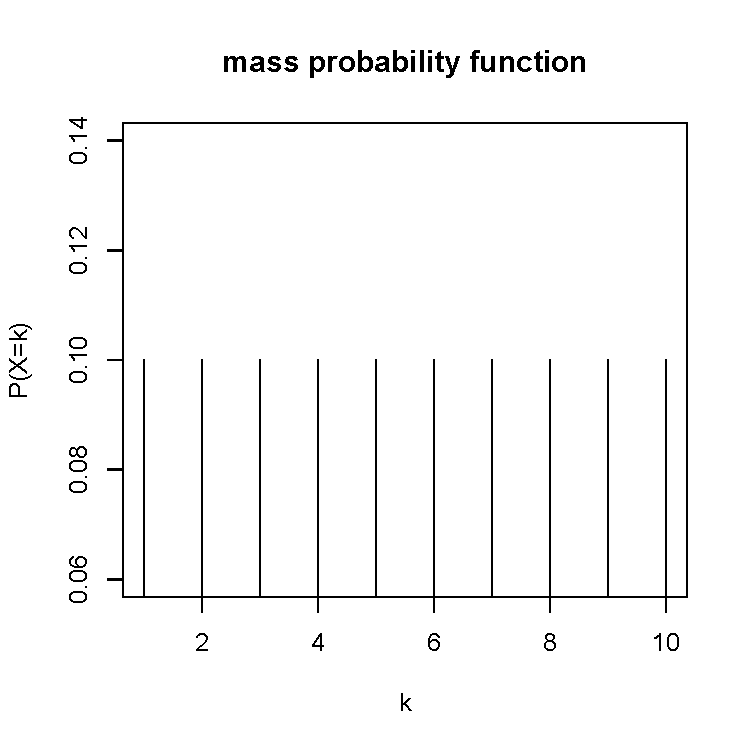
\includegraphics[width=0.48\textwidth]{img/discretunifzoom}
  \end{center}
  \vspace{-20pt}  
  \caption{Mass probability function for discrete uniform distribution}
  \vspace{-20pt}  
\end{wrapfigure}

The discrete uniform distribution can be defined in terms of its elementary distribution
(sometimes called mass probability function):
$$
P(X=k) = \frac{1}{n},
$$
where $k\in S=\{k_1, \dots, k_n\}$ (a finite set of ordered values). Typically, the $k_i$'s are consecutive positive integers.

Equivalenty, we have the following cumulative distribution function:
$$
F(k) = \frac{1}{n} \sum_{i=1}^n \ind_{(k_i\leq k)},
$$
where $\ind$ is the indicator function.

Furthermore, the probability generating function is given by
$$
G(t) \stackrel{\triangle}{=} E(t^X) = \frac{1}{n} \sum_{i=1}^n t^{k_i},
$$
with the special cases where the  $k_i$'s are $\{1,\dots,n\}$, we get
$$
G(t) = z \frac{1-z^n}{1-z},
$$
when  $z\neq 1$.

Finally, the \emph{moment} generating function is expressed as follows
$$
M(t) \stackrel{\triangle}{=} E(t^X) = \frac{1}{n} \sum_{i=1}^n e^{tk_i},
$$
with the special case $e^t \frac{1-e^{tn}}{1-e^t}$ when $S=\{1,\dots,n\}$.


\subsection{Properties}
The expectation is $\overline X_n$, the empirical mean: $ E(X)=\frac{1}{n} \sum_{i=1}^n k_i$.
When $S=\{1,\dots,n\}$, this is just $\frac{n+1}{2}$. The variance is given by $Var(X)=\frac{1}{n} \sum_{i=1}^n (k_i-E(X)^2$ which is $\frac{n^2-1}{12}$ for $S=\{1,\dots,n\}$.

\subsection{Estimation}
Since there is no parameter to estimate, calibration is pretty easy. But we need to 
check that sample values are equiprobable.

\subsection{Random generation}
The algorithm is simply
\begin{itemize}
\item generate $U$ from a uniform distribution,
\item compute the generated index as $I = \lceil n\times U  \rceil$,
\item finally $X$ is $k_I$.
\end{itemize}
where $\lceil . \rceil$ denotes the upper integer part of a number.

\subsection{Applications}
A typical application of the uniform discrete distribution is the statistic procedure called bootstrap or others resampling methods, where the previous algorithm is used.

%%%%%%%%%%%%%%%%%%%%%%%%%%%%%%%%%%%%%%%%%%%%%%%%%
\section{Bernoulli/Binomial distribution}
\subsection{Characterization}
\begin{wrapfigure}{r}{0.5\textwidth}
  \vspace{-20pt}
  \begin{center}
    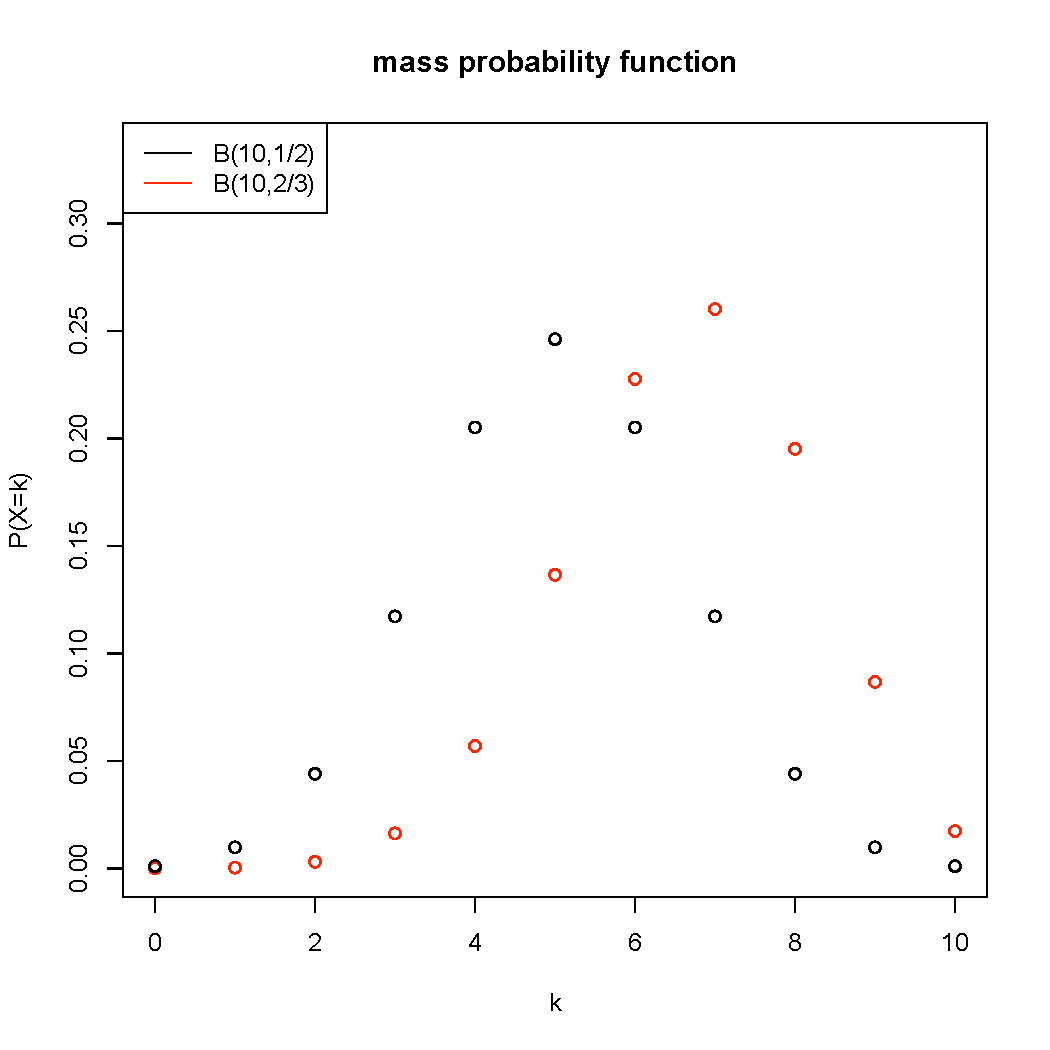
\includegraphics[width=0.48\textwidth]{img/binomzoom}
  \end{center}
  \vspace{-20pt}  
  \caption{Mass probability function for binomial distributions}
  \vspace{-20pt}  
\end{wrapfigure}


Since the Bernoulli distribution is a special case of the binomial distribution, we start by explaining the binomial distribution. The mass probability distribution is 
$$
P(X=k) = C_n^k p^k(1-p)^{n-k},
$$
where $C_n^k$ is the combinatorial number $\frac{n!}{k!(n-k)!}$, $k\in \mathbb N$ and $0<p<1$ the 'success' probability. Let us notice that the cumulative distribution function has no particular expression. In the following, the binomial dsitribuion
is denoted by $\mathcal B(n,p)$. A special case of the binomial dsitribution is the Bernoulli when $n=1$.
This formula explains the name of this distribution since elementary probabilities $P(X=k)$ are terms
of the development of $(p+(1-p))^n$ according the Newton's binom formula.

Another way to define the binomial distribution is to say that's the sum of $n$ identically and independently Bernoulli distribution $\mathcal B(p)$. Demonstration can easily be done with probability generating function.
The probability generating function is
$$
G(t) = (1-p+pz)^n,
$$
while the moment generating function is
$$
M(t) = (1-p+pe^t)^n.
$$

The binomial distribution assumes that the events are binary, mutually exclusive, independent and randomly selected.


\subsection{Properties}
The expectation of the binomial distribution is then $E(X) =np$ and its variance $Var(X)=np(1-p)$. A useful property is that a sum of binomial distributions is still binomial if success probabilities are the same, i.e.
$\mathcal B(n_1, p) + \mathcal B(n_2, p) \stackrel{\mathcal L}{=} \mathcal B(n_1+ n_2, p)$.

We have an asymptotic distribution for the binomial distribution. If $n\rightarrow +\infty$ and $p\rightarrow 0$ such that $np$ tends to a constant, then $\mathcal B(n,p) \rightarrow \mathcal P(np)$.

\subsection{Estimation}
\subsubsection{Bernoulli distribution}
Let $(X_i)_{1\leq i\leq m}$ be an i.i.d. sample of binomial distributions $\mathcal B(n,p)$. If $n=1$ (i.e. Bernoulli distribution, we have 
$$
\hat p_m = \frac{1}{m} \sum_{i=1}^m X_i
$$
is the unbiased and efficient estimator of $p$ with minimum variance. It is also the moment-based estimator.

There exists a confidence interval for the Bernoulli distribution using the Fischer-Snedecor distribution. We have
$$
I_\alpha(p) = \left[ \left(1+\frac{m-T+1}{T} f_{2(m-T+1),2T,\frac{\alpha}{2}}\right)^{-1} , \left(1+\frac{m-T}{T+1} f_{2(m-T),2(T+1),\frac{\alpha}{2}}\right)^{-1} \right],
$$
where $T=\sum_{i=1}^m X_i$ and $f_{\nu_1,\nu_2,\alpha}$ the $1-\alpha$ quantile of the Fischer-Snedecor distribution with $\nu_1$ and $\nu_2$ degrees of freedom.

We can also use the central limit theorem to find an asymptotic confidence interval for $p$
$$
I_\alpha(p) = \left[\hat p_m - \frac{u_\alpha}{\sqrt n} \sqrt{\hat p_m(1-\hat p_m)}, \hat p_m + \frac{u_\alpha}{\sqrt n} \sqrt{\hat p_m(1-\hat p_m)} \right],
$$
where $u_\alpha$ is the $1-\alpha$ quantile of the standard normal distribution.

\subsubsection{Binomial distribution}

When $n$ is not 1, there are two cases: either $n$ is known with certainty or $n$ is unknown.
In the first case, the estimator of $p$ is the same as the Bernoulli distribution. In the latter case, there are no closed form for the maximum likelihood estimator of $n$.

One way to solve this problem is to set $\hat n$ to the maximum number of 'success' at first. Then we compute the log likelihood for wide range of integers around the maximum and finally choose the likeliest value for $n$. 

Method of moments for $n$ and $p$ is easily computable. Equalling the 2 first sample moments, we
have the following solution
$$
\left\{
\begin{array}{l}
\tilde p = 1-\frac{S_m^2}{\bar X_m}\\
\tilde n = \frac{\bar X_m}{\tilde p} 
\end{array}
\right. ,
$$
with the constraint that $\tilde n\in \mbb N$.

Exact confidence intervals cannot be found since estimators do not have analytical form. But we can use the normal approximation for $\hat p$ and $\hat n$.



\subsection{Random generation}
It is easy to simulate Bernoulli distribution with the following heuristic:
\begin{itemize}
\item generate $U$ from a uniform distribution,
\item compute $X$ as 1 if $U\leq p$ and 0 otherwise.
\end{itemize}
The binomial distribution is obtained by summing $n$ i.i.d. Bernoulli random variates.

\subsection{Applications}
The direct application of the binomial distribution is to know the probability of obtaining exactly $n$ heads if a fair coin is flipped $m>n$ times. Hundreds of books deal with this application.

In medecine, the article \cite{nejm} presents an application of the binomial distribution to test for a particular syndrome.

In life actuarial science, the binomial distribution is useful to model the death of an insured or the entry in invalidity/incapability of an insured.

%%%%%%%%%%%%%%%%%%%%%%%%%%%%%%%%%%%%%%%%%%%%%%%%%
\section{Zero-truncated or zero-modified binomial distribution}
\subsection{Characterization}
\begin{wrapfigure}{r}{0.5\textwidth}
 \vspace{-1.5cm}
  \begin{center}
    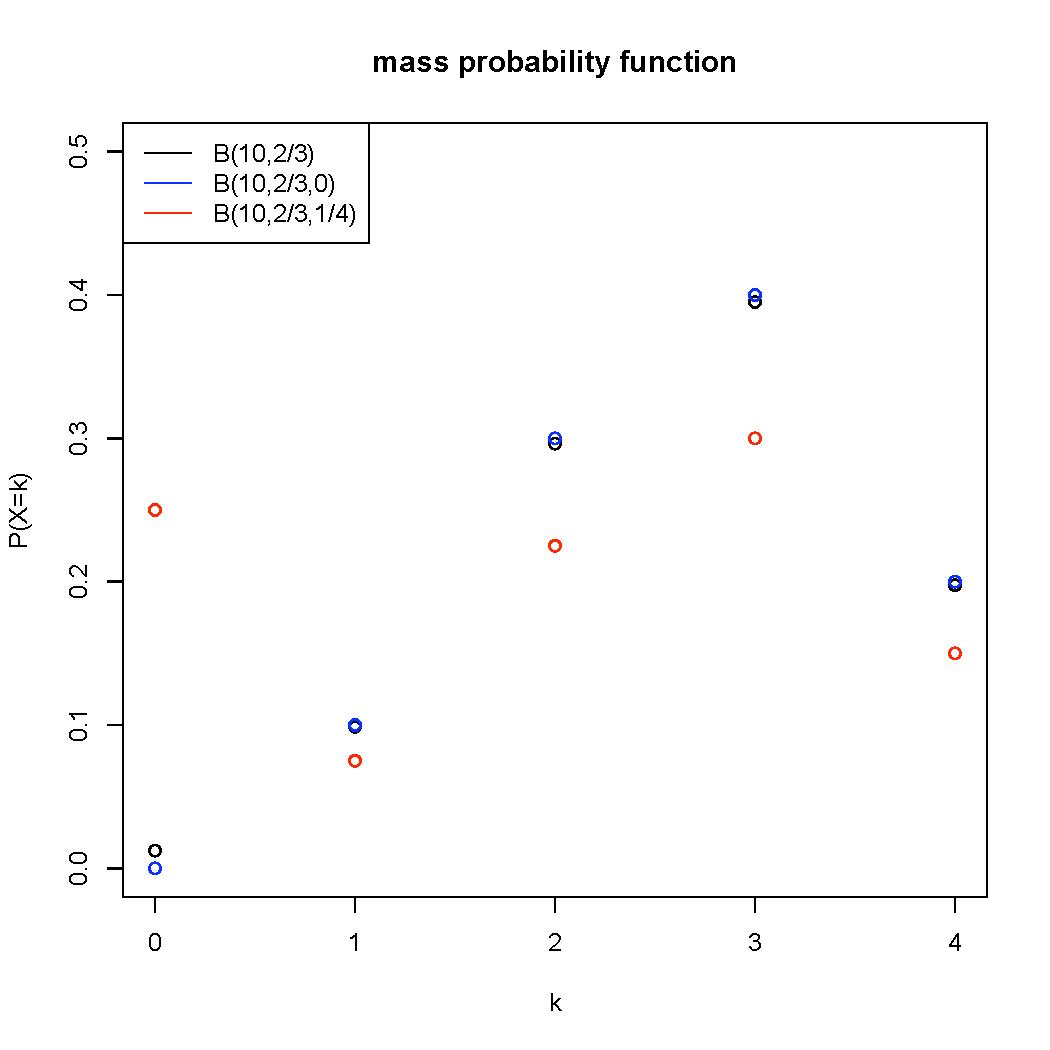
\includegraphics[width=0.48\textwidth]{img/truncbinomzoom}
  \end{center}
  \caption{Mass probability function for zero-modified binomial distributions}
\end{wrapfigure}

The zero-truncated version of the binomial distribution is defined as follows
$$
P(X=k)=\frac{C_n^k p^k (1-p)^{n-k}}{1-(1-p)^n},
$$
where $k\in \{1,\dots,n\}$, $n,p$ usual parameters. The distribution function does not have particular form. But the probability generating function and the moment generating function exist
$$
G(t) = \frac{(1+p(z-1))^n-(1-p)^n}{1-(1-p)^n},
$$
and 
$$
M(t)=\frac{(1+p(e^t-1))^n-(1-p)^n}{1-(1-p)^n}.
$$
In the following distribution, we denote the zero-truncated version by $\mcal B_0(n,p)$.

For the zero-modified binomial distribution, which of course generalizes the zero-truncated version, we have the following elementary probabilities
$$
P(X=k)=\left\{
\begin{array}{ll}
\tilde p &\txtm{if} k=0\\
KC_n^k p^k(1-p)^{n-k}  &\txtm{otherwise}\\
\end{array}
\right.
,
$$
where $K$ is the constant $\frac{1-\tilde p}{1-(1-p)^n}$, $n,p, \tilde p$ are the parameters. In terms of probability/moment generating functions we have:
$$
G(t)=\tilde p + K((1 - p + pz)^n-(1-p)^n) \txtm{and} M(t) = \tilde p + K((1 - p + pe^t)^n-(1-p)^n).
$$
The zero-modified binomial distribution is denoted by $\mcal B(n,p,\tilde p)$.

\subsection{Properties}
The expectation and the variance for the zero-truncated version is $E(X) = \frac{np}{1-(1-p)^n}$ and $Var(X)=\frac{np(1-p-(1-p+np)(1-p)^n)}{(1-(1-p)^n)^2}$. For the zero-modified version, we have $E(X)=Knp$ and $Var(X)=Knp(1-p)$.

\subsection{Estimation}
%\subsubsection{Zero-truncated version}
From \cite{cacoullos}, we know there is no minimum variance unbiased estimator for $p$. NEED HELP for the MLE... NEED \cite{thomasgart}

Moment based estimators are numerically computable whatever we suppose $n$ is known or unknown. 

Confidence intervals can be obtained with bootstrap methods.



\subsection{Random generation}
The basic algorithm for the zero-truncated version $\mcal B_0(n,p)$ is simply
\begin{itemize}
\item \textbf{do}; generate $X$ binomially distributed $\mcal B(n,p)$; \textbf{while} $X=0$
\item return $X$	
\end{itemize}
In output, we have a random variate in $\{1,\dots,n\}$.

The zero-modified version $\mcal B(n,p,\tilde p)$ is a little bit tricky. We need to use the following heuristic:
\begin{itemize}
\item generate $U$ from an uniform distribution
\item if $U< \tilde p$, then $X=0$
\item otherwise 
	\begin{itemize}
	\item \textbf{do}; generate $X$ binomially distributed $\mcal B(n,p)$; \textbf{while} $X=0$
	\end{itemize}
\item return $X$	
\end{itemize}


\subsection{Applications}
Human genetics???

%%%%%%%%%%%%%%%%%%%%%%%%%%%%%%%%%%%%%%%%%%%%%%%%%
\section{Quasi-binomial distribution}
\subsection{Characterization}
The quasi-binomial distribution is a ``small'' pertubation of the binomial distribution. The mass probability function is defined by
$$
P(X=k) = C_n^k p(p+k\phi)^{k-1}(1-p-k\phi)^{n-k},
$$
where $k\in \{0,\dots, n\}$, $n,p$ usual parameters and $\phi\in]-\frac{p}{n},\frac{1-p}{n}[$. Of course, we retrieve the binomial distribution with $\phi$ set to 0.

\subsection{Properties}
NEED REFERENCE
\subsection{Estimation}
NEED REFERENCE
\subsection{Random generation}
NEED REFERENCE
\subsection{Applications}
NEED REFERENCE

%%%%%%%%%%%%%%%%%%%%%%%%%%%%%%%%%%%%%%%%%%%%%%%%%
\section{Poisson distribution}
\subsection{Characterization}
\begin{wrapfigure}{r}{0.5\textwidth}
  \vspace{-20pt}
  \begin{center}
    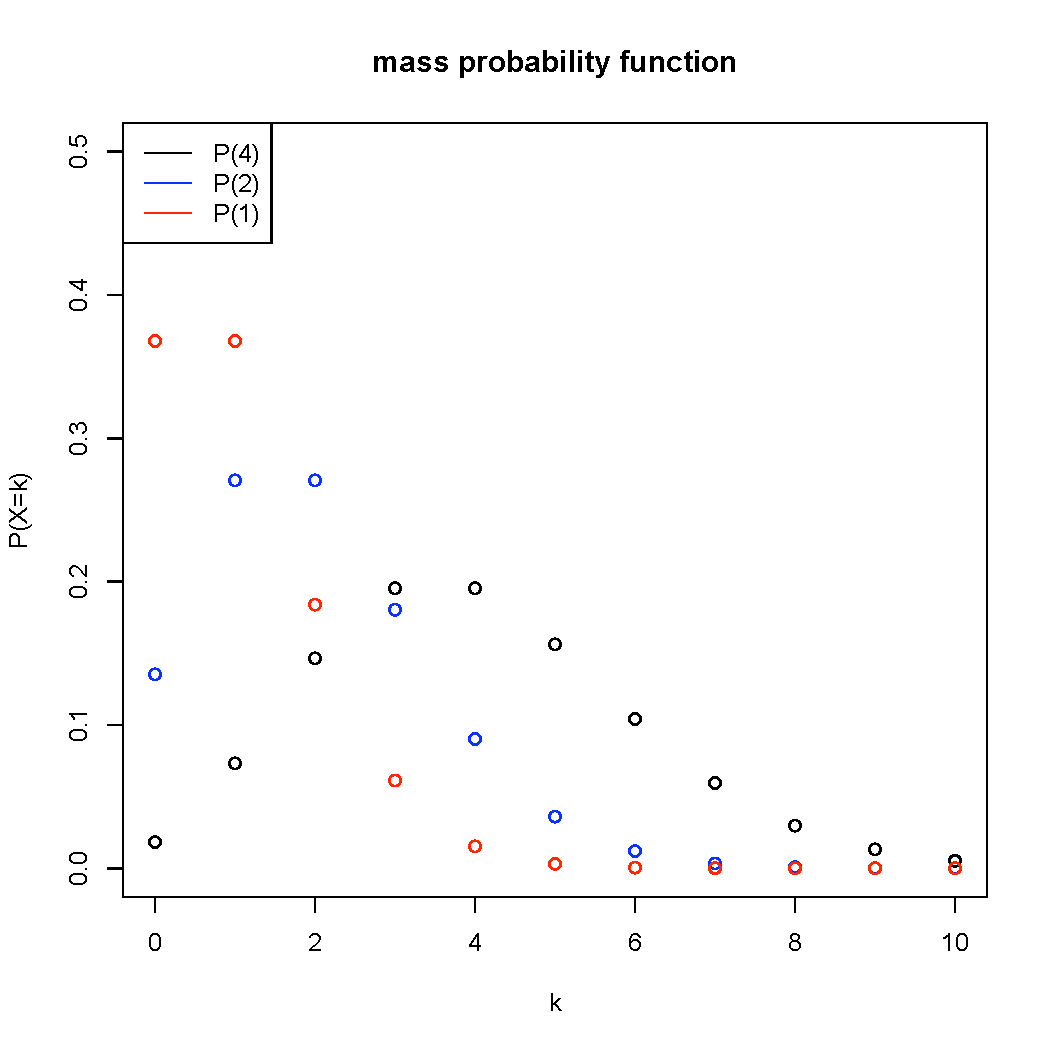
\includegraphics[width=0.48\textwidth]{img/poissonzoom}
  \end{center}
  \vspace{-20pt}
  \caption{Mass probability function for Poisson distributions}
  \vspace{-20pt}
\end{wrapfigure}

The Poisson distribution is characterized by the following elementary probabilities
$$
P(X=k) = \frac{\lambda^k}{k!}e^{-\lambda},
$$
where $\lambda>0$ is the shape parameter and $k\in\mathbb N$.

The cumulative distribution function has no particular form, but the probability generating function is
given by
$$
G(t) = e^{\lambda(t-1)},
$$
and the moment generating function is
$$
M(t) = e^{\lambda(e^t-1)}.
$$

Another way to characterize the Poisson distribution is to present the Poisson process (cf. \cite{saporta}). We consider independent and identically events occuring on a given period of time $t$. We assume that those events can not occur simultaneously and their probability to occur \emph{only} depends on the observation period $t$. Let $c$ be the average number of events per unit of time ($c$ for cadency). We can prove that the number of events $N$ occuring during the period $[0,t[$ is 
$$
P(N=n) = \frac{(ct)^k}{k!}e^{-ct},
$$
since the interoccurence are i.i.d. positive random variables with the property of 'lack of memory'\footnote{i.e. interoccurence are exponentially distributed, cf. the exponential distribution.}.

\subsection{Properties}
The Poisson distribution has the 'interesting' but sometimes annoying property to have the same mean and variance. We have $E(X) = \lambda = Var(X)$.

The sum of two independent Poisson distributions $\mathcal P(\lambda)$ and $\mathcal P(\mu)$ (still) follows a Poisson distribution $\mathcal P(\lambda+\mu)$.

Let $N$ follows a Poisson distribution $\mathcal P(\lambda)$. Knowing the value of $N=n$, let $(X_i)_{1\leq i\leq n}$ be a sequence of i.i.d. Bernoulli variable $\mathcal B(q)$, then $\sum_{i=1}^nX_i$
follows a Poisson distribution $\mathcal P(\lambda q)$.


\subsection{Estimation}
The estimator maximum likelihood estimator of $\lambda$ is $\hat \lambda = \overline X_n$ for a sample $(X_i)_i$. It is also the moment based estimator, an unbiased estimator $\lambda$ and an efficient estimator.

From the central limit theorem, we have asymptotic confidence intervals
$$
I_\alpha(\lambda) = \left[\hat \lambda_n - \frac{u_\alpha}{\sqrt n} \sqrt{\hat \lambda_m} , \hat \lambda_n + \frac{u_\alpha}{\sqrt n} \sqrt{\hat \lambda_m} \right],
$$
where $u_\alpha$ is the $1-\alpha$ quantile of the standard normal distribution.

\subsection{Random generation}
A basic way to generate Poisson random variate is the following:
\begin{itemize}
\item initialize variable $n$ to 0, $l$ to $e^{-\lambda}$ and $P$ to 1,
\item \textbf{do} 
	\begin{itemize}
	\item generate $U$ from a uniform distribution,
	\item $P = P \times U$,
	\item $n=n+1$,
	\end{itemize}
	\textbf{while} $P\geq l$, 
\item return $n-1$.
\end{itemize}
See \cite{knuth02} for details.

 

TOIMPROVE

Ahrens, J. H. and Dieter, U. (1982). Computer generation of Poisson deviates from modified normal distributions. ACM Transactions on Mathematical Software, 8, 163?179.

\subsection{Applications}
TODO


%%%%%%%%%%%%%%%%%%%%%%%%%%%%%%%%%%%%%%%%%%%%%%%%%
\section{Zero-truncated or zero-modified Poisson distribution}
\subsection{Characterization}
\begin{wrapfigure}{r}{0.5\textwidth}
  \vspace{-20pt}
  \begin{center}
    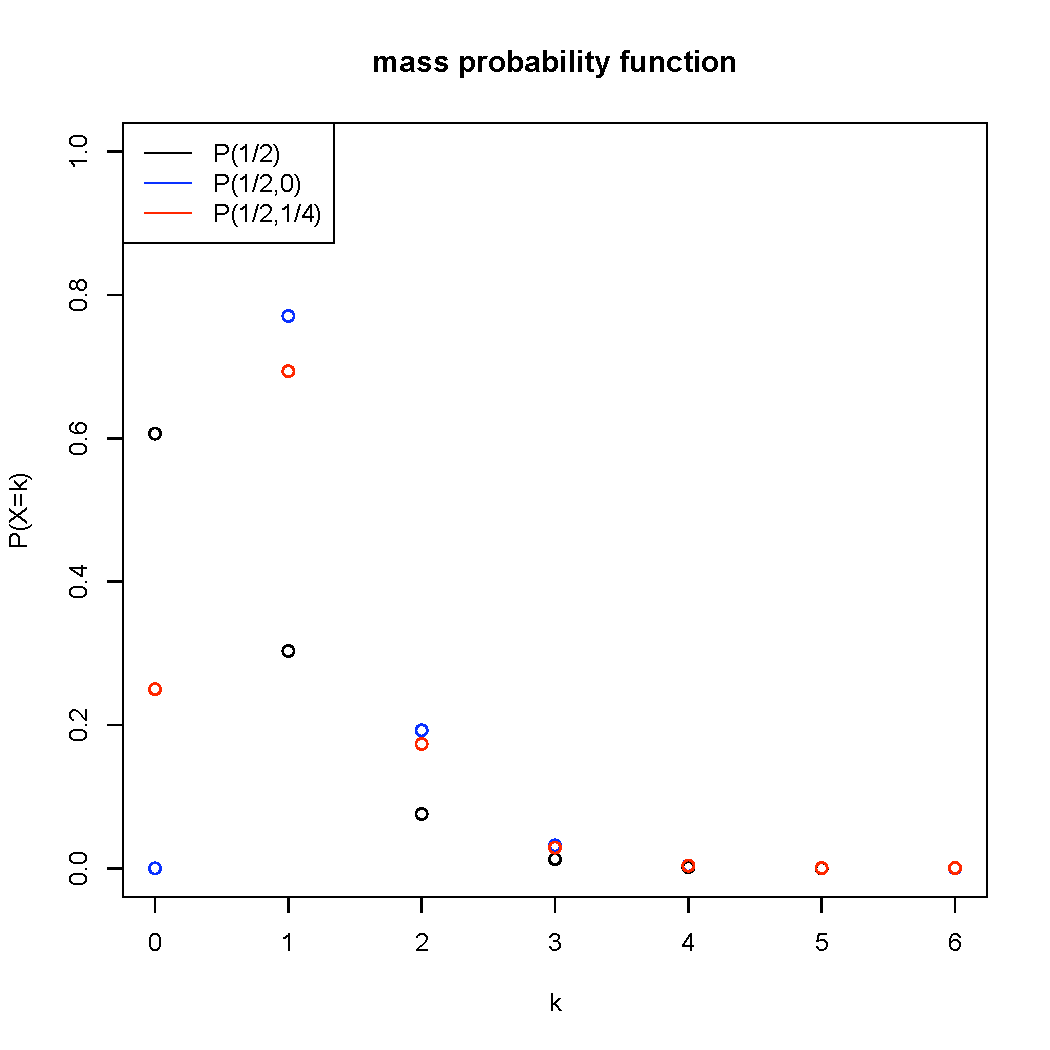
\includegraphics[width=0.48\textwidth]{img/truncpoissonzoom}
  \end{center}
  \vspace{-20pt}
  \caption{Mass probability function for zero-modified Poisson distributions}
  \vspace{-20pt}
\end{wrapfigure}

The zero-truncated version of the Poisson distribution is defined the zero-truncated binomial distribution for the Poisson distribution. The elementary probabilities is defined as
$$
P(X=k)=\frac{\lambda^k}{k!}\frac{1}{(e^\lambda-1)},
$$
where $k\in \mbb N^*$.
We can define probability/moment generating functions for the zero-truncated Poisson distribution $\mcal P_0(\lambda)$:
$$
G(t) = \frac{e^{\lambda t}-1}{e^\lambda-1} \txtm{and} M(t) =\frac{e^{\lambda e^t}-1}{e^\lambda-1}.
$$

The zero-modified version of the Poisson distribution (obviously) generalized the zero-truncated version. We have the following mass probability function
$$
P(X=k)=\left\{
\begin{array}{ll}
p & \txtm{if} k=0\\
K\frac{\lambda^k}{k!} e^{-\lambda} & \txtm{otherwise}
\end{array}
\right.
,
$$
where $K$ is the constant $\frac{1-p}{1-e^{-\lambda}}$. The ``generating functions'' for the zero-modified Poisson distribution $\mcal P(\lambda, p)$ are
$$
G(t)=p+K(e^{\lambda t}-1) \txtm{and} M(t)=p+K(e^{\lambda e^t}-1).
$$


\subsection{Properties}
The expectation of the zero-truncated Poisson distribution is $E(X)=\frac{\lambda}{1-e^{-\lambda}}$ and $K\lambda$ for the zero-modified version. While the variance are respectively $Var(X)=\frac{\lambda}{(1-e^{-\lambda})^2}$ and $K \lambda+(K-K^2)\lambda^2$.

\subsection{Estimation}
\subsubsection{Zero-truncated Poisson distribution}
Let $(X_i)_i$ be i.i.d. sample of truncated Poisson random variables.
Estimators of $\lambda$ for the zero-truncated Poisson distribution are studied in \cite{tategoen}. Here is the list of possible estimators for $\lambda$:
\begin{itemize}
\item $\tilde \lambda = \frac{T}{n}(1-\frac{{}_2S_{n-1}^{t-1}}{{}_2S_{n}^{t}})$ is the minimum variance unbiased estimator,
\item $ \lambda^* = \frac{T}{n}(1-\frac{N_1}{T})$ is the Plackett's estimator,
\item $\hat\lambda$, the solution of equation $\frac{T}{n}=\frac{\lambda}{1-e^{-\lambda}}$, is the maximum likelihood estimator,
\end{itemize}
where $T=\sum_{i=1}^nX_i$, ${}_2S_{n}^{k}$ denotes the Stirling number of the second kind and $N_1$ the number of observations equal to 1. Stirling numbers are costly do compute, see \cite{tategoen} for approximate of theses numbers.

\subsubsection{Zero-modified Poisson distribution}
NEED REFERENCE

\subsection{Random generation}
The basic algorithm for the zero-truncated version $\mcal P_0(\lambda)$ is simply
\begin{itemize}
\item \textbf{do}; generate $X$ Poisson distributed $\mcal P(\lambda)$; \textbf{while} $X=0$
\item return $X$	
\end{itemize}
In output, we have a random variate in $\mbb N^*$.

The zero-modified version $\mcal P(\lambda, p)$ is a little bit tricky. We need to use the following heuristic:
\begin{itemize}
\item generate $U$ from an uniform distribution
\item if $U< p$, then $X=0$
\item otherwise 
	\begin{itemize}
	\item \textbf{do}; generate $X$ Poisson distributed $\mcal P(\lambda)$; \textbf{while} $X=0$
	\end{itemize}
\item return $X$	
\end{itemize}

\subsection{Applications}
NEED REFERENCE

%%%%%%%%%%%%%%%%%%%%%%%%%%%%%%%%%%%%%%%%%%%%%%%%%
\section{Quasi-Poisson distribution}
NEED FOLLOWING REFERENCE

Biom J. 2005 Apr;47(2):219-29.
    Generalized Poisson distribution: the property of mixture of Poisson and comparison with negative binomial distribution.
    Joe H, Zhu R.

    
Ecology. 2007 Nov;88(11):2766-72.
    Quasi-Poisson vs. negative binomial regression: how should we model overdispersed count data?
    Ver Hoef JM, Boveng PL.

 
    
\subsection{Characterization}
TODO
\subsection{Properties}
TODO
\subsection{Estimation}
TODO
\subsection{Random generation}
TODO
\subsection{Applications}

%%%%%%%%%%%%%%%%%%%%%%%%%%%%%%%%%%%%%%%%%%%%%%%%%
\section{Geometric distribution}
\subsection{Characterization}
\begin{wrapfigure}{r}{0.5\textwidth}
  \vspace{-20pt}
  \begin{center}
    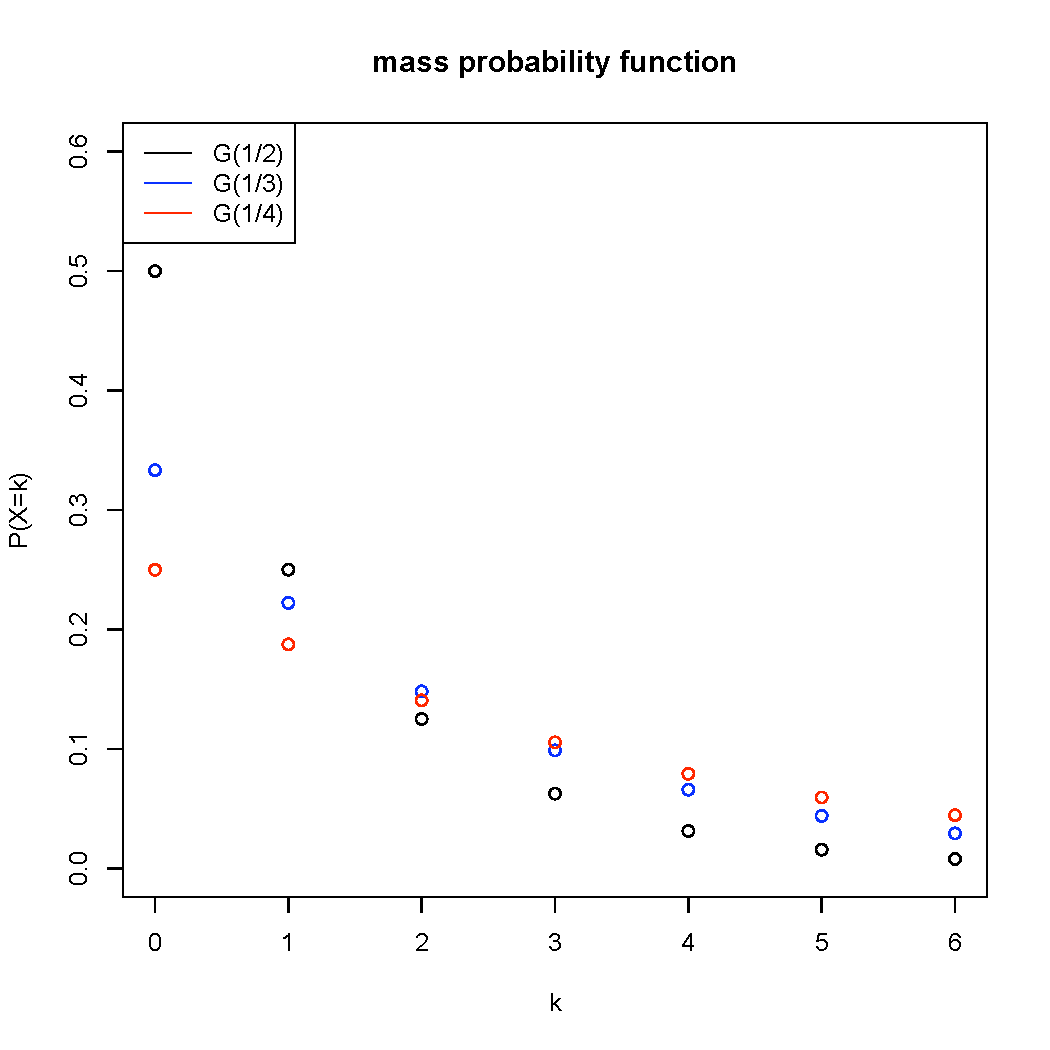
\includegraphics[width=0.48\textwidth]{img/geomzoom}
  \end{center}
  \vspace{-20pt}
  \caption{Mass probability function for Geometric distributions}

\end{wrapfigure}
The geometric distribution represents the first outcome of a particular event (with the probability $q$ to raise) in a serie of i.i.d. events. The mass probability function is 
$$
P(X=k) = q(1-q)^{k},
$$
where $k\in\mathbb N$ and $0<q\leq 1$. In terms of cumulative distribution function, it is the same as
$$
F(k) = 1- (1-q)^{k+1}.
$$
The whole question is wether this outcome could be null or at least one (event). 
If we consider the distribution to be valued in $\mathbb N^*$, please see the truncated geometric distribution.

The probability generating function of the geometric $\mathcal G(q)$ is
$$
G(t) = \frac{q}{1-(1-q)t},
$$ 
and its moment generating function 
$$
M(t) = \frac{q}{1-(1-q)e^t}.
$$

\subsection{Properties}
The expecation of a geometric distribution is simply $E(X)=\frac{1-q}{q}$ and its variance $Var(X)=\frac{1-q}{q^2}$.

The sum of $n$ i.i.d. geometric $\mathcal G(q)$ random variables follows a negative binomial distribution $\mathcal N\mcal B(n,q)$.

The minimum of $n$ independent geometric $\mcal G(q_i)$ random variables follows a geometric distribution $\mcal G(q_.)$ with $q_. = 1-\prod_{i=1}^n (1-q_i)$. 

The geometric distribution is the discrete analogue of the exponential distribution thus it is memoryless. 

\subsection{Estimation}
The maximum likelihood estimator of $q$ is $\hat q = \frac{1}{1+\bar X_n}$, which is also the moment based estimator.

NEED REFERENCE



\subsection{Random generation}
A basic algorithm is to use i.i.d. Bernoulli variables as follows
\begin{itemize}
\item initialize $X$ to 0 and generate $U$ from an uniform distribution,
\item \textbf{while} $U>p$ \textbf{do} ; generate $U$ from an uniform distribution; $X=X+1$; 
\item return $X$.
\end{itemize}
TOIMPROVE WITH 
Devroye, L. (1986) Non-Uniform Random Variate Generation. Springer-Verlag, New York. Page 480. 

\subsection{Applications}
NEED MORE REFERENCE THAN \cite{macutek} 

%%%%%%%%%%%%%%%%%%%%%%%%%%%%%%%%%%%%%%%%%%%%%%%%%
\section{Zero-truncated or zero-modified geometric distribution}
\subsection{Characterization}
\begin{wrapfigure}{r}{0.5\textwidth}
  \vspace{-30pt}
  \begin{center}
    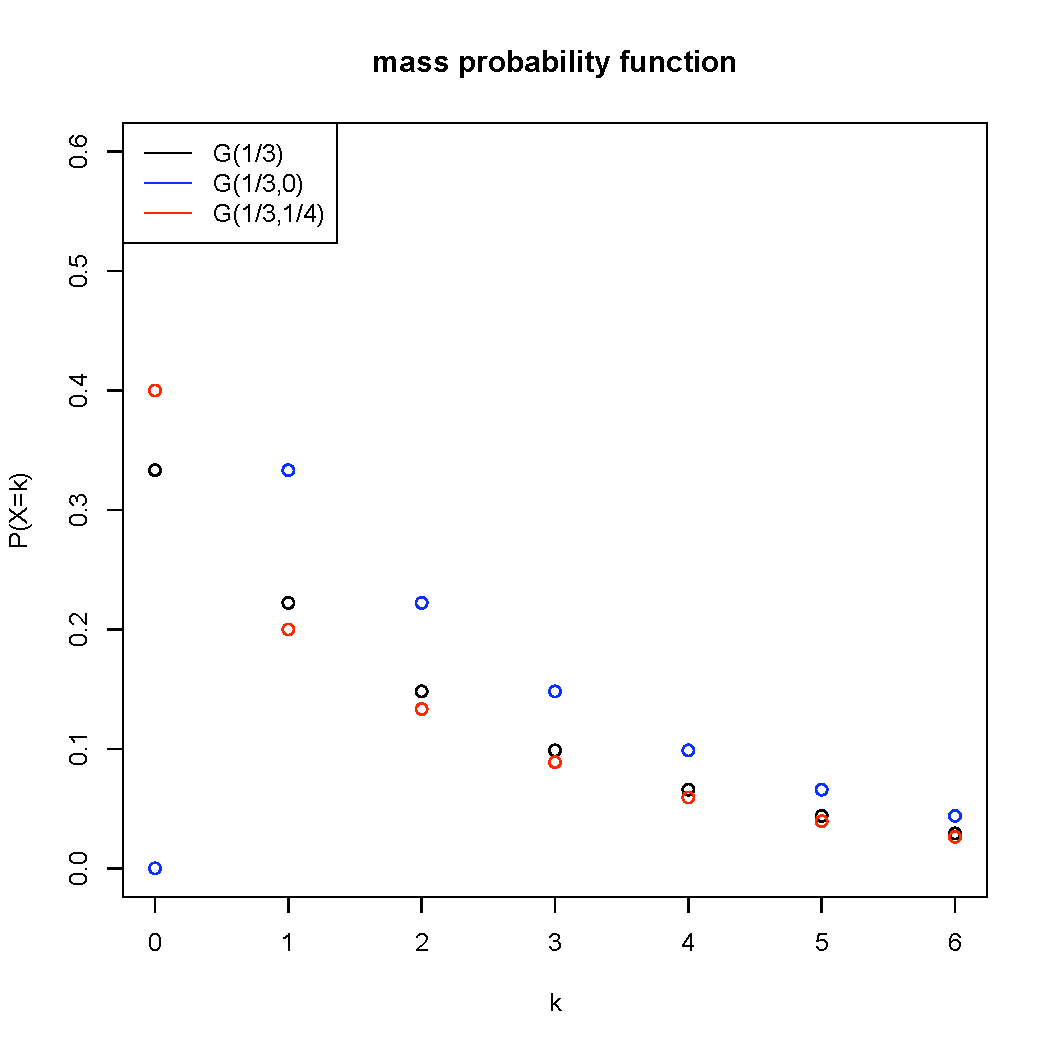
\includegraphics[width=0.48\textwidth]{img/truncgeomzoom}
  \end{center}
  \caption{Mass probability function for zero-modified geometric distributions}
\end{wrapfigure}

The zero-truncated version of the geometric distribution is defined as
$$
P(X=k) = p(1-p)^{k-1},
$$
where $n\in\mathbb N^+$. Obviously, the distribution takes values in $\{1,\dots, n,\dots\}$.
Its distribution function is 
$$
F(k) = 1-(1-p)^k.
$$
Finally the probability/moment generating functions are
$$
G(t) = \frac{pt}{1-(1-p)t}, \txtm{and} M(t) = \frac{pe^t}{1-(1-p)e^t}.
$$
In the following, it is denoted by $\mathcal G_0(p)$.

The zero-modified version of the geometric distribution is characterized as follows
$$
P(X=k) = \left\{
\begin{array}{ll}
p & \txtm{if} k=0\\
Kq(1-q)^k & \txtm{otherwise}\\
\end{array}
\right. ,
$$
where the constant $K$ is $\frac{1-p}{1-q}$ and $k\in\mathbb N$.
Of course special cases of the zero modified version of the geometric $\mathcal G(q,p)$ are the zero-truncated version with $p=0$ and $q=p$ and the classic geometric distribution with $p=q$. The distribution function is expressed as follows
$$
F(x) = p+K(1-(1-p)^k),
$$
where $k\geq 0$. The probability/moment generating functions are 
$$
G(t) = p+K\left(\frac{q}{1-(1-q)t}-q\right) \txtm{and} M(t) =p+K\left(\frac{q}{1-(1-q)e^{t}}-q\right).
 $$

\subsection{Properties}
The expectation of the geometric $\mathcal G_0(p)$ distribution is $E(X)=\frac{1}{p}$ and its variance $Var(X)=\frac{1-p}{p^2}$.

For the zero-modified geometric distribution $\mathcal G(q,p)$, we have $E(X) = K\frac{1-q}{q}$ and $Var(X)=K\frac{1-q}{q^2}$.

\subsection{Estimation}
\subsubsection{Zero-truncated geometric distribution}
According to \cite{cacoullos}, the (unique) minimim variance unbiased estimator of $q$ for the zero-truncated geometric distribution is 
$$
\tilde q = t \frac{\tilde S_n^{t-1}}{\tilde S_n^t},
$$
where $t$ denotes the sum $\sum_{i=1}^n X_i$, $\tilde S_n^t$ is defined by $\frac{1}{n!}\sum_{k=1}^n(-1)^{n-k} C_n^k(k+t-1)_t$\footnote{where $C_n^k$'s are the binomial coefficient and $(n)_m$ is the falling factorial.}. The maximum likelihood estimator of $q$ is given by
$$
\hat q = \frac{1}{\bar X_n},
$$
which is also the moment based estimator. By the uniqueness of the unbiased estimator, $\hat q$ is a biased estimator.

\subsubsection{Zero-modified geometric distribution}
Moment based estimators for the zero-modified geometric distribution $\mcal G(p,q)$ are given by
$\hat q = \frac{\bar X_n}{S_n^2}$ and $\hat p = 1-\frac{(\bar X_n)^2}{S_n^2}$.

NEED REFERENCE

\subsection{Random generation}
For the zero-truncated geometric distribution, a basic algorithm is to use i.i.d. Bernoulli variables as follows
\begin{itemize}
\item initialize $X$ to 1 and generate $U$ from an uniform distribution,
\item \textbf{while} $U>q$ \textbf{do} ; generate $U$ from an uniform distribution; $X=X+1$; 
\item return $X$.
\end{itemize}

While for the zero-modified geometric distribution, it is a little bit tricky
\begin{itemize}
\item generate $U$ from an uniform distribution
\item if $U< p$, then $X=0$
\item otherwise 
	\begin{itemize}
         \item initialize $X$ to 1 and generate $U$ from an uniform distribution
	\item \textbf{while} $U>q$ \textbf{do} ; generate $U$ from an uniform distribution; $X=X+1$;
	\end{itemize}
\item return $X$	
\end{itemize}

\subsection{Applications}
NEED REFERENCE

%%%%%%%%%%%%%%%%%%%%%%%%%%%%%%%%%%%%%%%%%%%%%%%%%
\section{Negative binomial distribution}
\subsection{Characterization}
\subsection{Characterization}
\begin{wrapfigure}{r}{0.5\textwidth}
  \vspace{-30pt}
  \begin{center}
    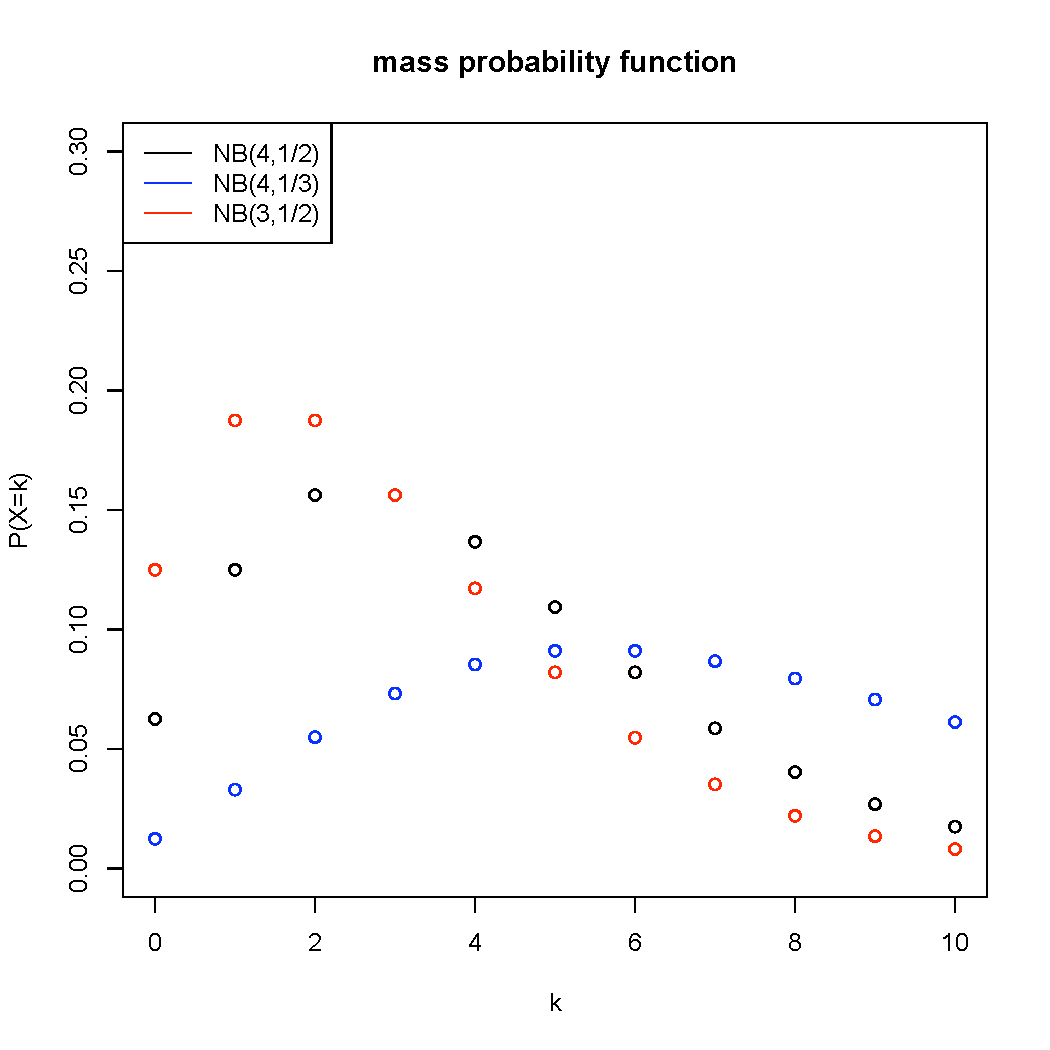
\includegraphics[width=0.48\textwidth]{img/negbinomzoom}
  \end{center}
  \caption{Mass probability function for negative binomial distributions}
\end{wrapfigure}

The negative binomial distribution can be characterized by the following mass probability function
$$
P(X=k) = C_{m+k-1}^{k} p^m(1-p)^{k},
$$
where $k\in\mathbb N$, $C_{m+k-1}^{k}$'s are combinatorial numbers and parameters $m,p$ are constraint by $0<p<1$ and $m\in\mathbb N^*$. However a second parametrization of the negative binomial distribution is
$$
P(X=k)=\frac{\Gamma(r+k)}{\Gamma(r)k!} \left(\frac{1}{1+\beta}\right)^r\left(\frac{\beta}{1+\beta}\right)^k,
$$
where $k\in\mathbb N$ and $r,\beta>0$. We can retrieve the first parametrization $\mathcal N\mathcal B(m,p)$ from the second parametrization $\mathcal N\mathcal B(r,\beta)$ with
$$
\left\{
\begin{array}{c}
\frac{1}{1+\beta} = p\\
r = m\\
\end{array}
\right.
$$

The probability generating functions for these two parametrizations are
$$
G(t)= \left(\frac{p}{1-(1-p)t}\right)^m \txtm{and} G(t)=\left(\frac{1}{1-\beta(t-1)}\right)^r,
$$
and their moment generating functions are 
$$
M(t)= \left(\frac{p}{1-(1-p)e^{t}}\right)^m \txtm{and} M(t) = \left(\frac{1}{1-\beta(e^t-1)}\right)^r.
$$

One may wonder why there are two parametrization for one distribution. Actually, the first parametrization $\mathcal N\mathcal B(m,p)$ has a meaningful construction: it is the sum of $m$ i.i.d. geometric $\mathcal G(p)$ random variables. So it is also a way to characterize a negative binomial distribution.
The name comes from the fact that the mass probability function can be rewritten as
$$
P(X=k) = C_{m+k-1}^{k} \left(\frac{1-p}{p}\right)^{k}\left(\frac{1}{p}\right)^{-m-k},
$$
which yields to
$$
P(X=k) = C_{m+k-1}^{k} P^{k}Q^{-m-k}.
$$
This is the general term of the development of $(P-Q)^{-m}$.
 

\subsection{Properties}
The expectation of negative binomial $\mathcal N\mathcal B(m,p)$ (or $\mathcal N\mathcal B(m,p)$) is $E(X) =  \frac{m(1-p)}{p}$ or ($r \beta$), while its variance is $Var(X)=\frac{m(1-p)}{p^2}$ or ($r\beta(1+\beta)$).

Let $N$ be Poisson distributed $\mathcal P(\lambda\Theta)$ knowing that $\Theta=\theta$ where $\Theta$ is gamma distributed $\mathcal G(a,a)$. Then we have $N$ is negative binomial distributed $\mathcal B\mathcal N(a,\frac{\lambda}{a})$. 



\subsection{Estimation}
Moment based estimators are given by $\hat \beta = \frac{S_n^2}{\bar X_n}-1$ and $\hat r = \frac{\bar X_n}{\hat \beta}$. 

NEED REFERENCE

\subsection{Random generation}
The algorithm to simulate a negative binomial distribution $\mcal N\mcal B(m,p)$ is simply to generate $m$ random variables geometrically distributed and to sum them.

NEED REFERENCE

\subsection{Applications}
From \cite{simon}, here are some applications of the negative binomial distribution
\begin{itemize}
\item number of bacterial colonies per microscopic field,
\item quality control problem,
\item claim frequency in non life insurance.
\end{itemize}

%%%%%%%%%%%%%%%%%%%%%%%%%%%%%%%%%%%%%%%%%%%%%%%%%
\section{Zero-truncated or zero-modified negative binomial distribution}
\subsection{Characterization}
The zero-truncated negative binomial distribution is characterized by
$$
P(X=k) = \frac{\Gamma(r+k)}{\Gamma(r)k!((r+\beta)^r-1)} (\frac{\beta}{1+\beta})^k,
$$
where $k\in \mbb N^*$, $r,\beta$ usual parameters. In terms of probability generating function,
we have
$$
G(t) =  \frac{(1-\beta(t-1))^r-(1+\beta)^{-r}}{1-(r+\beta)^r}.
$$ 

The zero-modified version is defined as follows
$$
P(X=k)=\left\{
\begin{array}{ll}
p & \txtm{if} k=0\\
K\frac{\Gamma(r+k)}{\Gamma(r)k!} (\frac{1}{1+\beta})^r(\frac{\beta}{1+\beta})^k & \txtm{otherwise}\\
\end{array}
\right. ,
$$
where $K$ is defined as $\frac{1-p}{1- (\frac{1}{1+\beta})^r}$, $r,\beta$ usual parameters and $p$ the new parameter. The probability generating function is given by
$$
G(t) = \left((\frac{1}{1-\beta(t-1)})^r-(\frac{1}{1+\beta})^r\right),
$$
and 
$$
M(t) = \left((\frac{1}{1-\beta(e^t-1)})^r-(\frac{1}{1+\beta})^r\right)
$$
for the moment generating function.

\subsection{Properties}
Expectations for these two distribution are $E(X) = \frac{ r \beta}{1-(r+\beta)^r}$ and $Kr \beta$ respectively for the zero-truncated and the zero-modified versions. Variances are $Var(X)=\frac{ r\beta(1+\beta -(1+\beta+r\beta)(1+\beta)^{-r} )}{(1-(r+\beta)^r)^2}$ and $ Kr\beta(1+\beta)+(K-K^2)E^2[X]$.

\subsection{Estimation}
According to \cite{cacoullos}, the (unique) minimim variance unbiased estimator of $p$ for the zero-truncated geometric distribution is 
$$
\tilde p = t \frac{\tilde S_{r,n}^{t-1}}{\tilde S_n^t},
$$
where $t$ denotes the sum $\sum_{i=1}^n X_i$, $\tilde S_n^t$ is defined by $\frac{1}{n!}\sum_{k=1}^n(-1)^{n-k} C_n^k(k+t-1)_t$\footnote{where $C_n^k$'s are the binomial coefficient and $(n)_m$ is the increasing factorial.}. The maximum likelihood estimator of $q$ is given by
$$
\hat q = \frac{1}{\bar X_n},
$$
which is also the moment based estimator. By the uniqueness of the unbiased estimator, $\hat q$ is a biased estimator.

\subsection{Random generation}
\subsection{Applications}

%%%%%%%%%%%%%%%%%%%%%%%%%%%%%%%%%%%%%%%%%%%%%%%%%
\section{Pascal distribution}
\subsection{Characterization}
The negative binomial distribution can be constructed by summing $m$ geometric distributed variables $\mathcal G(p)$. The Pascal distribution is got from summing $n$ geometrically distributed $\mathcal G_0(p)$ variables. Thus possible values of the Pascal distribution are in $\{n, n+1,\dots\}$. The mass probability function is defined as
$$
P(X=k) = C_{k-1}^{n-1} p^n(1-p)^{k-n} ,
$$
where $k\in \{n, n+1, \dots \}$, $n\in \mathbb N^*$ and $0<p<1$. The probability/moment generating functions are 
$$
G(t) = \left(\frac{pt}{1-(1-p)t}\right)^n \txtm{and} M(t) =\left(\frac{pe^{t}}{1-(1-p)e^{t}}\right)^n.
 $$

\subsection{Properties}
For the Pascal distribution $\mathcal Pa(n,p)$, we have
$E(X) = \frac{n}{p}$ and $Var(X)=\frac{n(1-p)}{p^2}$. The link between Pascal distribution $\mathcal Pa(n,p)$ and the negative binomial distribution $\mathcal B\mathcal N(n,p)$ is to substract the constant $n$, i.e. if $X\sim \mathcal Pa(n,p)$ then $X-n\sim \mathcal B\mathcal N(n,p)$.
\subsection{Estimation}
\subsection{Random generation}
\subsection{Applications}

%%%%%%%%%%%%%%%%%%%%%%%%%%%%%%%%%%%%%%%%%%%%%%%%%
\section{Hypergeometric distribution}
\subsection{Characterization}
The hypergeometric distribution is characterized by the following elementary probabilities
$$
P(X=k) =\frac{C_m^kC_{N-m}^{n-k}}{C_N^n},
$$
where $N\in\mathbb N^+$, $(m,n)\in\{1,\dots, N\}^2$ and $k\in \{0,\dots,\min(m,n)\}$. 

It can also be defined though its probability generating function or moment generating function:
$$
G(t) = \frac{C_{N-m}^n\,_2F_1 (-n,-m;N-m-n+1; t) }{C_N^n} \txtm{and} M(t) =\frac{C_{N-m}^n \,_2F_1 (-n,-m;N-m-n+1;e^t)}{C_N^n},
$$
where $\,_2F_1$ is the hypergeometric function of second kind.

\subsection{Properties}
The expectation of an hypergeometric distribution is $E(X) = \frac{nm}{N}$ and $Var(X)=\frac{nm(N-n)(N-m)}{N^2(N-1)}$.

We have the following asymptotic result: $\mathcal H(N,n,m) \mapsto \mathcal B(n,\frac{m}{N})$ when $N$ and $m$ are large such that $\frac{m}{N} \underset{N\rightarrow +\infty}{\longrightarrow} 0<p<1$.

\subsection{Estimation}
\subsection{Random generation}
\subsection{Applications}
Let $N$ be the number of individuals in a given population. In this population, $m$ has a particular property, hence a proportion of $\frac{m}{N}$. If we draw $n$ individuals among this population, the random variable associated with the number of people having the desired property follows a hypergeometric distribution $\mathcal H(N,n,m)$. The ratio $\frac{n}{N}$ is called the survey rate.

%----------------------------------------------------------------------------------------------------------
% 	Copyright (c) 2009 R-forge 'distributions' Core Team, 
% 	
%	The following Sweave code is under the GNU Free Documentation License:
%      	Permission is granted to copy, distribute and/or modify this document
%      	under the terms of the GNU Free Documentation License, Version 1.3
%      	or any later version published by the Free Software Foundation;
%      	with no Invariant Sections, no Front-Cover Texts, and no Back-Cover Texts.
%
%      A copy of the license is included in the 'inst' directory of this package 
%      or on the web at http://www.gnu.org/licenses/licenses.html#FDL
%
%	After running Sweave, the following code could be compiled :
%	  - on windows with a Tex distribution such as miktex (http://miktex.org) 
%		and a front end Latex editor such as texniccenter (http://www.toolscenter.org)
%	  - on mac os with a Tex distribution such as TexLive and a front end Latex
%	  	editor such as Texshop (http://www.uoregon.edu/~koch/texshop/)
%	  - on linux with a Tex distribution such as teTex (http://www.tug.org/teTeX/)
%	  	and a front end Latex editor such as emacs (http://www.gnu.org/software/emacs/)
%
%----------------------------------------------------------------------------------------------------------


\chapter{Not so-common discrete distribution}
\section{Conway-Maxwell-Poisson distribution}
\subsection{Characterization}
TODO
\subsection{Properties}
TODO
\subsection{Estimation}
TODO
\subsection{Random generation}
TODO
\subsection{Applications}

\section{Delaporte distribution}
\subsection{Characterization}
TODO
\subsection{Properties}
TODO
\subsection{Estimation}
TODO
\subsection{Random generation}
TODO
\subsection{Applications}

\section{Engen distribution}
\subsection{Characterization}
TODO
\subsection{Properties}
TODO
\subsection{Estimation}
TODO
\subsection{Random generation}
TODO
\subsection{Applications}


\section{Logaritmic distribution}
\subsection{Characterization}
TODO
\subsection{Properties}
TODO
\subsection{Estimation}
TODO
\subsection{Random generation}
TODO
\subsection{Applications}

\section{Sichel distribution}
\subsection{Characterization}
TODO
\subsection{Properties}
TODO
\subsection{Estimation}
TODO
\subsection{Random generation}
TODO
\subsection{Applications}



\section{Zipf distribution}
The name ``Zipf distribution'' comes from George Zipf's work on the discretized version of the Pareto distribution, cf. \cite{arnold83}.
\subsection{Characterization}
See Arnold(83) for relationship with Pareto's distribution.
\subsection{Properties}
TODO
\subsection{Estimation}
TODO
\subsection{Random generation}
TODO
\subsection{Applications}

\section{The generalized Zipf distribution}
\subsection{Characterization}
TODO
\subsection{Properties}
TODO
\subsection{Estimation}
TODO
\subsection{Random generation}
TODO
\subsection{Applications}

\section{Rademacher distribution}
\subsection{Characterization}
TODO
\subsection{Properties}
TODO
\subsection{Estimation}
TODO
\subsection{Random generation}
TODO
\subsection{Applications}

\section{Skellam distribution}
\subsection{Characterization}
TODO
\subsection{Properties}
TODO
\subsection{Estimation}
TODO
\subsection{Random generation}
TODO
\subsection{Applications}

\section{Yule distribution}
\subsection{Characterization}
TODO
\subsection{Properties}
TODO
\subsection{Estimation}
TODO
\subsection{Random generation}
TODO
\subsection{Applications}

\section{Zeta distribution}
\subsection{Characterization}
TODO
\subsection{Properties}
TODO
\subsection{Estimation}
TODO
\subsection{Random generation}
TODO
\subsection{Applications}


\part{Continuous distributions}
%----------------------------------------------------------------------------------------------------------
% 	Copyright (c) 2009 R-forge 'distributions' Core Team, 
% 	
%	The following Sweave code is under the GNU Free Documentation License:
%      	Permission is granted to copy, distribute and/or modify this document
%      	under the terms of the GNU Free Documentation License, Version 1.3
%      	or any later version published by the Free Software Foundation;
%      	with no Invariant Sections, no Front-Cover Texts, and no Back-Cover Texts.
%
%      A copy of the license is included in the 'inst' directory of this package 
%      or on the web at http://www.gnu.org/licenses/licenses.html#FDL
%
%	After running Sweave, the following code could be compiled :
%	  - on windows with a Tex distribution such as miktex (http://miktex.org) 
%		and a front end Latex editor such as texniccenter (http://www.toolscenter.org)
%	  - on mac os with a Tex distribution such as TexLive and a front end Latex
%	  	editor such as Texshop (http://www.uoregon.edu/~koch/texshop/)
%	  - on linux with a Tex distribution such as teTex (http://www.tug.org/teTeX/)
%	  	and a front end Latex editor such as emacs (http://www.gnu.org/software/emacs/)
%
%----------------------------------------------------------------------------------------------------------

\chapter{Finite support distribution}
%%%%%%%%%%%%%%%%%%%%%%%%%%%%%%%%%%%%%%%%%%
\section{Uniform distribution}
\subsection{Characterization}
\begin{wrapfigure}{r}{0.5\textwidth}
  \vspace{-20pt}
  \begin{center}
    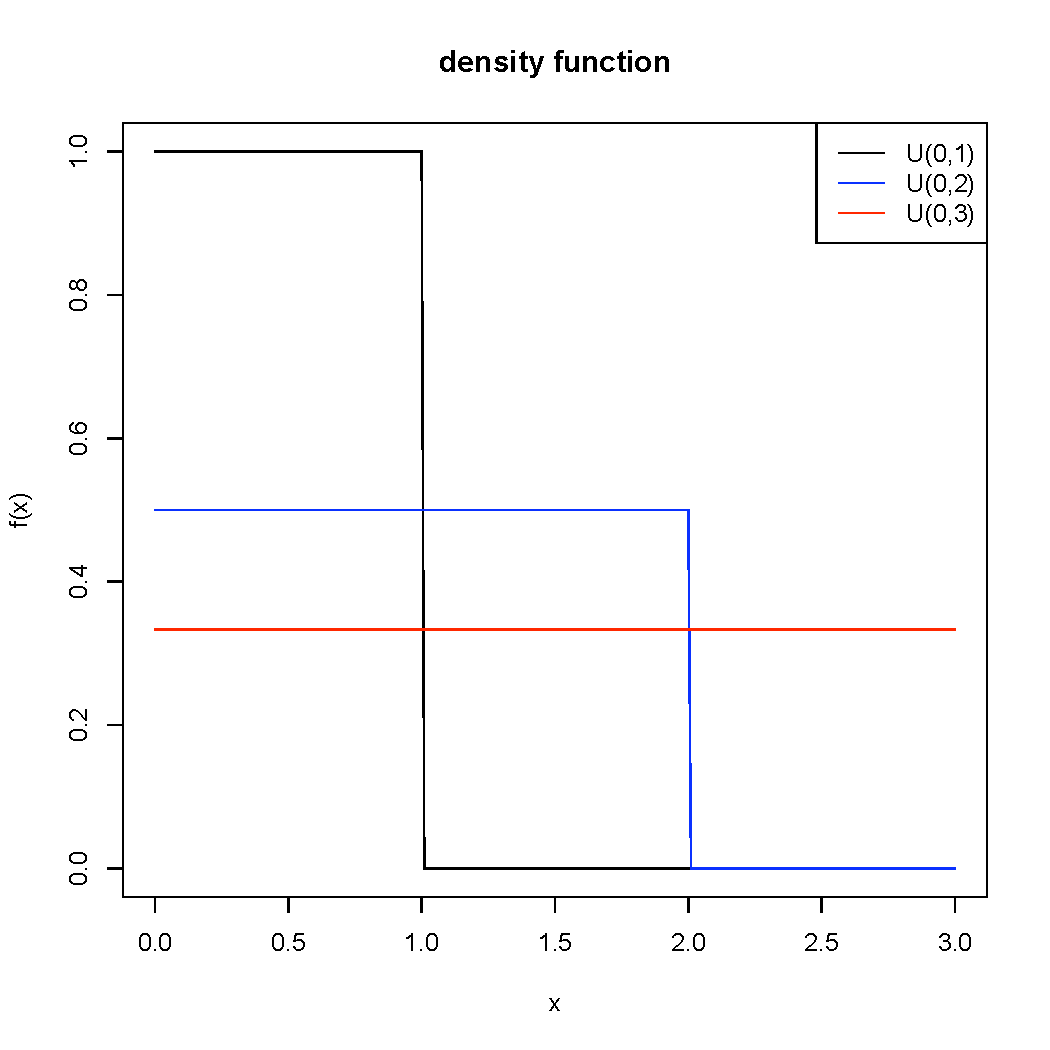
\includegraphics[width=0.48\textwidth]{img/unifzoom}
  \end{center}
  \vspace{-20pt}  
  \caption{Density function for uniform distribution}
  \vspace{-20pt}  
\end{wrapfigure}

The uniform distribution is the most intuitive distribution, its density function is 
$$
f(x) = \frac{1}{b-a},
$$
where $x\in [a,b]$ and $a<b\in \mathbb R$. So the uniform $\mathcal U(a,b)$ is only valued in $[a,b]$.
From this, we can derive the following distribution function
$$
F(x) = \left\{
\begin{array}{ll}
0 & \txtm{if} x<a\\
\frac{x-a}{b-a} & \txtm{if} a\leq x\leq b\\
1 & \txtm{otherwise}\\
\end{array}
\right. .
$$

Another way to define the uniform distribution is to use the moment generating function
$$
M(t) = \frac{e^{tb}-e^{ta}}{t(b-a)}
$$
whereas its characteristic function is 
$$
\phi(t) = \frac{e^{ibt}-e^{iat}}{i(b-a)t}.
$$

\subsection{Properties}
The expectation of a uniform distribution is $E(X) = \frac{a+b}{2}$ and its variance $Var(X)=\frac{(b-a)^2}{12}.$

If $U$ is uniformally distributed $\mathcal U(0,1)$, then $(b-a) \times U + a$ follows a uniform distribution $\mathcal U(a,b)$.

The sum of two uniform distribution does not follow a uniform distribution but a triangle distribution.

The order statistic $X_{k:n}$ of a sample of $n$ i.i.d. uniform $\mcal U(0,1)$ random variable is beta distributed $\mcal Beta(k, n-k+1)$.

Last but not least property is that for all random variables $Y$ having a distribution function $F_Y$, the random variable $F_Y(Y)$ follows a uniform distribution $\mathcal U(0,1)$. Equivalently, we get that the random variable $F_Y^{-1}(U)$ has the same distribution as $Y$ where $U\sim \mathcal U(0,1)$ and $F_Y^{-1}$ is the generalized inverse distribution function. Thus, we can generate any random variables having a distribution from the a uniform variate. This methods is called the inverse function method.


\subsection{Estimation}
For a sample $(X_i)_i$ of i.i.d. uniform variate, maximum likelihood estimators for $a$ and $b$ are respectively $X_{1:n}$ and $X_{n:n}$, where $X_{i:n}$ denotes the order statistics. But they are biased so we can use the following unbiased estimators
$$
\hat a = \frac{n}{n^2-1} X_{1:n} + \frac{1}{1-n^2}X_{n:n} \txtm{and}
\hat b = \frac{1}{1-n^2} X_{1:n} + \frac{n}{n^2-1}X_{n:n}.
$$
Finally the method of moments gives the following estimators
$$
\tilde a = \bar X_n -\sqrt{3 S_n^2} \txtm{and} \tilde b = \bar X_n +\sqrt{3 S_n^2}.
$$

\subsection{Random number generation}
Since this is the core distribution, the distribution can not be generated from another distribution. In our modern computers, we use deterministic algorithms to generate uniform variate initialized with the machine time. Generally, Mersenne-Twister algorithm (or its extensions) from \cite{matsumoto98} is implemented, cf. \cite{dutangc08} for an overview of random number generation.

\subsection{Applications}
The main application is sampling from an uniform distribution by the inverse function method.


%%%%%%%%%%%%%%%%%%%%%%%%%%%%%%%%%%%%%%%%%%
\section{Triangular distribution}
\subsection{Characterization}
\begin{wrapfigure}{r}{0.5\textwidth}
  \vspace{-20pt}
  \begin{center}
    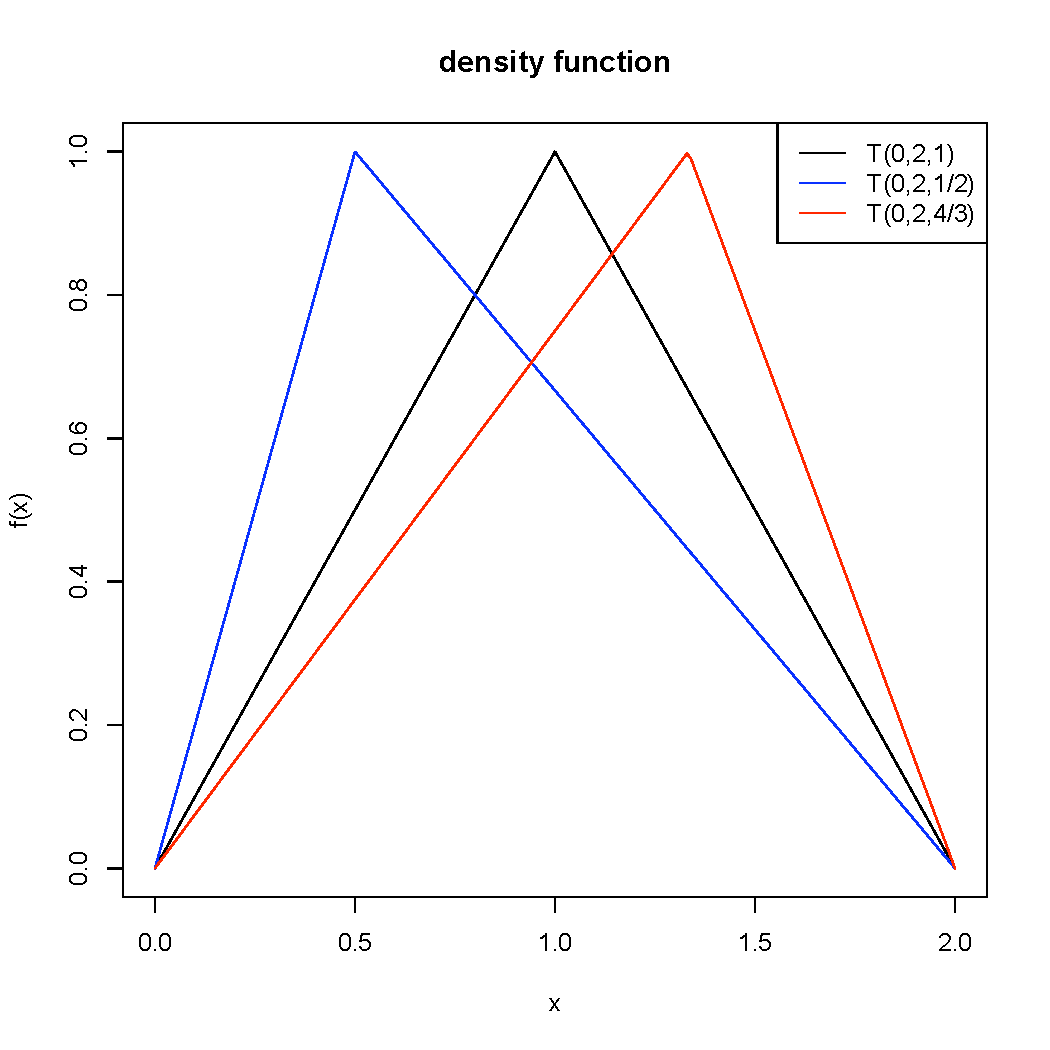
\includegraphics[width=0.48\textwidth]{img/trianglezoom}
  \end{center}
  \vspace{-20pt}  
  \caption{Density function for triangular distributions}
\end{wrapfigure}

The triangular distribution has the following density
$$
f(x) = \left\{
\begin{array}{ll}
\frac{2(x-a)}{(b-a)(c-a)} & \txtm{if} a\leq x\leq c\\
\frac{2(b-x)}{(b-a)(b-c)} & \txtm{if}c\leq x\leq b
\end{array}
\right. ,
$$
where $x\in[a,b]$, $a\in\mathbb R$, $a < b$ and $a\leq c\leq b$. The associated distribution function
is
$$
F(x) = \left\{
\begin{array}{ll}
\frac{(x-a)^2}{(b-a)(c-a)} & \txtm{if} a\leq x\leq c\\
1-  \frac{(b-x)^2}{(b-a)(b-c)} & \txtm{if}c\leq x\leq b
\end{array}
\right. .
$$

As many finite support distribution, we have a characteristic function and a moment generating function. They have the following expresion:
$$
\phi(t) = \frac{(b-c)e^{iat}-(b-a)e^{ict}}{-2(b-a)(c-a)(b-c)t^2}+\frac{-2(c-a)e^{ibt}}{(b-a)(c-a)(b-c)t^2} 
$$
and
$$
M(t) = \frac{(b-c)e^{at}-(b-a)e^{ct}}{2(b-a)(c-a)(b-c)t^2}+\frac{2(c-a)e^{bt}}{(b-a)(c-a)(b-c)t^2}.
$$



\subsection{Properties}
The expectation of the triangle distribution is $E(X) = \frac{a+b+c}{3}$ whereas its variance is $Var(X) = \frac{a^2+b^2+c^2}{18}-\frac{ab+ac+bc}{18}$.

\subsection{Estimation}
Maximum likelihood estimators for $a$, $b$, $c$ do not have closed form. But we can maximise the log-likelihood numerically. Furthermore, moment based estimators have to be computed numerically solving the system of sample moments and theoretical ones. One intuitive way to estimate the parameters of the triangle distribution is to use sample minimum, maximum and mode:
$\hat a = X_{1:n}$, $\hat b=X_{n:n}$ and $\hat c = \textrm{mode}(X_1,\dots,X_n)$, where $\textrm{mode}(X_1,\dots,X_n)$ is the middle of the interval whose bounds are the most likely order statistics.

\subsection{Random generation}
The inverse function method can be used since the quantile function has a closed form:
$$
F^{-1}(u) = \left\{
\begin{array}{ll}
a+\sqrt{u(b-a)(c-a)} & \txtm{if} 0\leq u\leq \frac{c-a}{b-a}\\
b-\sqrt{(1-u)(b-a)(b-c)} & \txtm{if} \frac{c-a}{b-a} \leq u \leq1\\
\end{array}
\right. .
$$
Thus $F^{-1}(U)$ with $U$ a uniform variable is triangular distributed.

\cite{steinkeblis} provides new kind of methods to simulate triangular variable. An algorithm for the triangular $\mcal T(0,1,c)$ distribution is provided. It can be adapted for $a,b,c$ in general. 
Let $\tilde c$ be $\frac{c-a}{b-a}$ which is in $]0,1[$. The ``minmax'' algorithm is
\begin{itemize}
\item generate $U,V$ (idependently) from a uniform distribution,
\item $X =  a+(b-a)\times\left[(1-\tilde c) \min(U,V) + \tilde c \max(U,V)\right]$.
\end{itemize}
This article also provides another method using a square root of uniform variate, which is called ``one line method'', but it is not necessary more fast if we use vector operation.

\subsection{Applications}
A typical of the triangle distribution is when we know the minimum and the maximum of outputs of an interest variable plus the most likely outcome, which represent the parameter $a, b$ and $c$. For example we may use it in business decision making based on simulation of the outcome, in project management to model events during an interval and in audio dithering.

%%%%%%%%%%%%%%%%%%%%%%%%%%%%%%%%%%%%%%%%%%%
\section{Beta type I distribution}
\subsection{Characterization}
\begin{wrapfigure}{r}{0.5\textwidth}
  \vspace{-20pt}
  \begin{center}
    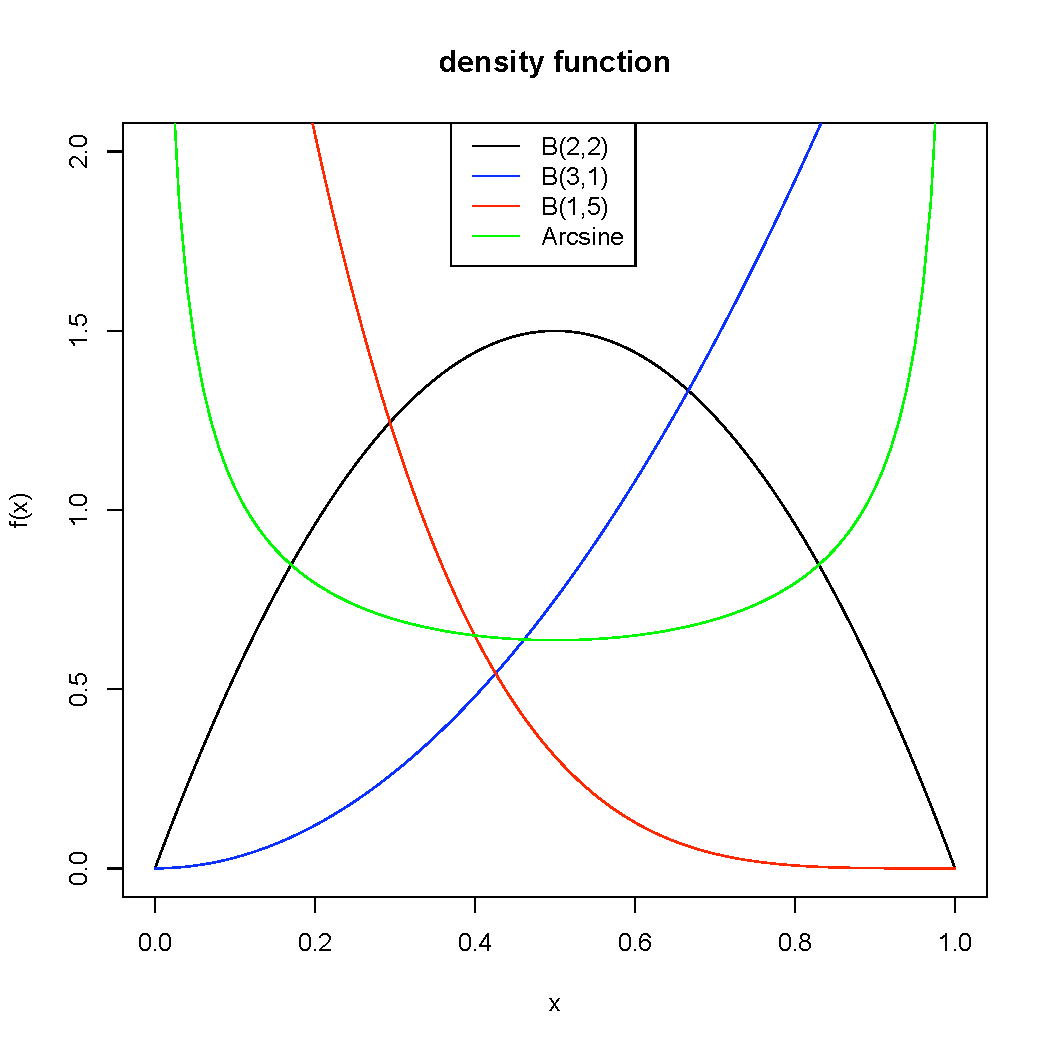
\includegraphics[width=0.48\textwidth]{img/betazoom}
  \end{center}
  \vspace{-20pt}  
  \caption{Density function for beta distributions}
\end{wrapfigure}
The beta distribution of first kind is a distribution valued in the interval $[0,1]$. Its density is defined as
$$
f(x) = \frac{x^{a-1} (1-x)^{b-1} }{\beta(a,b)},
$$
where $x\in [0,1]$, $a,b>0$ and $\beta(.,.)$ is the beta function defined in terms of the gamma function.

Since $a,b$ can take a wide range of values, this allows many different shapes for the beta density:
\begin{itemize}
\item $a=b=1$ corresponds to the uniform distribution
\item when $a,b<1$, density is U-shapped
\item when $a<1$, $b\geq 1$ or $a=1$, $b>1$, density is strictly decreasing
	\begin{itemize}
	\item for $a=1,b>2$, density is strictly convex
	\item for $a=1, b=2$, density is a straight line
	\item for $a=1, 1<b<2$, density is strictly concave
	\end{itemize}
\item when $a=1, b<1$ or $a>1, b\leq 1$, density is strictly increasing 	\begin{itemize}
	\item for $a>2,b=1$, density is strictly convex
	\item for $a=2, b=1$, density is a straight line
	\item for $1<a<2, b=1$, density is strictly concave
	\end{itemize}
\item when $a,b>1$, density is unimodal.
\end{itemize}
Let us note that $a=b$ implies a symmetric density.

From the density, we can derive its distribution function
$$
F(x) = \frac{\beta(a,b,x)}{\beta(a,b)},
$$
where $x\in [0,1]$ and $\beta(.,.,.)$ denotes the incomplete beta function. There is no analytical formula for the incomplete beta function but can be approximated numerically.

There exists a scaled version of the beta I distribution. Let $\theta$ be a positive scale parameter. The density of the scaled beta I distribution is given by
$$
f(x) = \frac{x^{a-1} (\theta-x)^{b-1} }{\theta^{a+b-1}\beta(a,b)},
$$
where $x\in [0,\theta]$. We have the following distribution function
$$
F(x) = \frac{\beta(a,b,\frac{x}{\theta})}{\beta(a,b)}.
$$

Beta I distributions have moment generating function and characteristic function expressed in terms of series:
$$
M(t)=1  +\sum_{k=1}^{+\infty} \left( \prod_{r=0}^{k-1} \frac{a+r}{a+b+r} \right) \frac{t^k}{k!}
$$
and
$$
\phi(t) = {}_1F_1(a; a+b; i\,t),
$$
where ${}_1F_1$ denotes the hypergeometric function.

\subsection{Special cases}

A special case of the beta I distribution is the arcsine distribution, when $a=b=\frac{1}{2}$. In this special case, we have
$$
f(x) = \frac{1}{\pi\sqrt{x(1-x)}},
$$
from which we derive the following distribution function
$$
F(x) = \frac{2}{\pi} \arcsin(\sqrt{x}).
$$

Another special case is the power distribution when $b=1$, with the following density
$$
f(x) = a x^{a-1}
\txtm{and}
F(x) = x^a,
$$
for $0<x<1$.

\subsection{Properties}
The moments of the beta I distribution are $E(X) = \frac{a}{a+b}$ and $Var(X)=\frac{ab}{(a+b)^2(a+b+1)}$ (and $\frac{\theta a}{a+b}$, $\frac{\theta^2ab}{(a+b)^2(a+b+1)}$ for the scaled version respectively).

Raw moments for the beta I distribution are given by
$$
E(X^r) = \frac{\Gamma(\alpha+\beta)\Gamma(\alpha+r)}{\Gamma(\alpha+\beta+r)\Gamma(\alpha)},
$$
while central moments have the following expression
$$
E\left((X-E(X))^r\right) = \left(-\frac{\alpha}{\alpha+\beta}\right)^r {}_2F_1 \left(\alpha, -r, \alpha+\beta,\frac{\alpha+\beta}{\alpha}\right).
$$

For the arcsine distribution, we have $\frac{1}{2}$ and $\frac{1}{8}$ respectively. Let us note that the expectation of a arcsine distribution is the least probable value!

Let $n$ be an integer. If we consider $n$ i.i.d. uniform $\mcal U(0,1)$ variables $U_i$, then the distribution of the maximum $\underset{1\leq i\leq n}{\max} U_i$ of these random variables follows a beta I distribution $\mcal B(n,1)$.



\subsection{Estimation}
Maximum likelihood estimators for $a$ and $b$ do not have closed form, we must solve the system
$$
\left\{
\begin{array}{l}
\frac{1}{n}\sum\limits_{i=1}^n\log(X_i) = \beta(a,b) (\psi(a+b)-\psi(a)) \\
\frac{1}{n}\sum\limits_{i=1}^n\log(1-X_i) = \beta(a,b) (\psi(a+b)-\psi(b)) \\
\end{array}
\right.
$$
numerically, where $\psi(.)$ denotes the digamma function.

Method of moments gives the following estimators
$$
\tilde a = \bar X_n \left(\frac{\bar X_n (1 - \bar X_n)}{S_n^2} - 1 \right)
\txtm{and}
\tilde b = \tilde a \frac{1-\bar X_n}{\bar X_n}.
$$

\subsection{Random generation}
NEED REFERENCE

\subsection{Applications}
The arcsine distribution (a special case of the beta I) can be used in game theory. If we have two players playint at head/tail coin game and denote by $(S_i)_{i\geq 1}$ the serie of gains of the first player for the different game events, then the distribution of the proportion of gains among all the $S_i$'s that are positive follows asymptotically an arcsine distribution.

%%%%%%%%%%%%%%%%%%%%%%%%%%%%%%%%%%%%%%%%%%
\section{Generalized beta I distribution}
\subsection{Characterization}
\begin{wrapfigure}{r}{0.5\textwidth}
  \vspace{-20pt}
  \begin{center}
    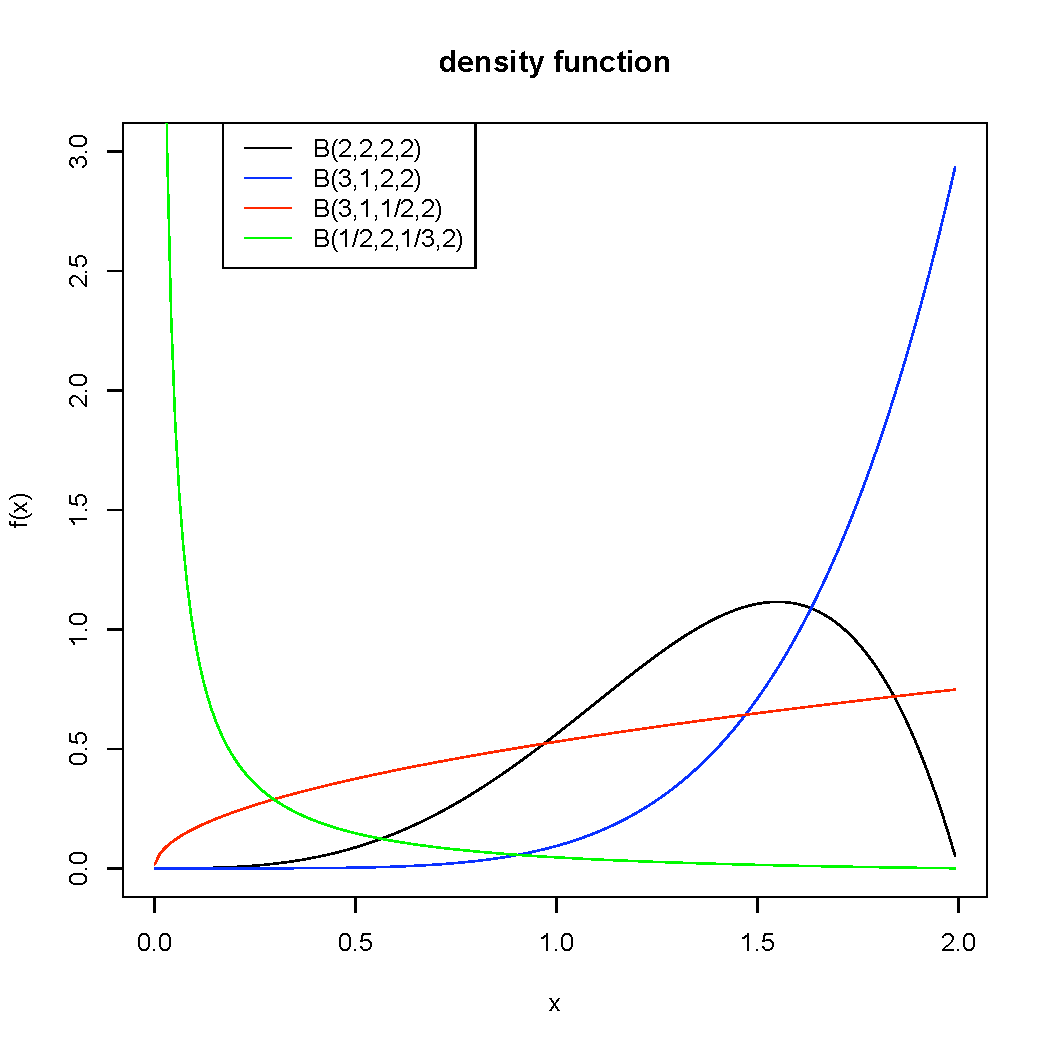
\includegraphics[width=0.48\textwidth]{img/genbetazoom}
  \end{center}
  \vspace{-20pt}  
  \caption{Density function for generalized beta distributions}
    \vspace{-20pt}  
\end{wrapfigure}

The generalized beta distribution is the distribution of the variable $\theta X^{\frac{1}{\tau}}$ when $X$ is beta distributed. Thus it has the following density
$$
f(x) = \frac{(x/\theta)^{a-1} (1-(x/\theta))^{b-1}}{ \beta(a,b)}   \frac{\tau}{x}
$$
for $0<x<\theta$ and $a, b, \tau, \theta>0$. $\theta$ is a scale parameter while $a, b, \tau$ are shape parameters.

As for the beta distribution, the distribution function is expressed in terms of the incomplete beta function
$$
F(x) = \frac{\beta(a,b,(\frac{x}{\theta})^\tau)}{\beta(a,b)},
$$
for $0<x<\theta$.

\subsection{Properties}
Moments of the generalized beta distribution are given by the formula
$$
E(X^r) = \theta^r \frac{\beta(a+\frac{r}{\tau})}{\beta(a,b)}.
$$

For $\tau=\theta=1$, we retrieve the beta I distribution.

\subsection{Estimation}
Maximum likelihood estimators as well as moment based estimators have no chance to have explicit form, but we can compute it numerically.
NEED REFERENCE

\subsection{Random generation}
NEED REFERENCE
\subsection{Applications}
NEED REFERENCE

%%%%%%%%%%%%%%%%%%%%%%%%%%%%%%%%%%%%%%%%%%
\section{Generalization of the generalized beta I distribution}
\subsection{Characterization}
A generalization of the generalized beta distribution has been studied in \cite{kotznadara}.
Its density is given by
$$
f(x) = \frac{b\beta(a,b)}{\beta(a,b+\gamma)} x^{a+b-1} {}_2F_1(1-\gamma, a, a+b,x),
$$
where $0<x<1$ and ${}_2F_1$ denotes the hypergeometric function.
Its distribution function is also expressed in terms of the hypergeometric function:
$$
F(x) = \frac{b\beta(a,b)}{(a+b)\beta(a,b+\gamma)} x^{a+b} {}_2F_1(1-\gamma, a, a+b+1,x),
$$

\subsection{Special cases}
\cite{kotznadara} list specials cases of this distribution:
If $a+b+\gamma=1$ then we get 
$$
f(x) = \frac{b\Gamma(b)x^{a+b-1}(1-x)^{-a}}{\Gamma(1-a)\Gamma(a+b)}.
$$
If $a+b+\gamma=2$ then we get
$$
f(x) = \frac{b(a+b-1)\beta(a,b)}{\beta(a,2-a)}\beta(a+b-1,1-a,x)
$$
If in addition
\begin{itemize}
\item  $a+b-1\in\mbb N$, we have
$$
f(x) = \frac{b(a+b-1)\beta(a,b)\beta(a+b-1,1-a)}{\beta(a,2-a)} \left(1- \sum_{i=1}^{a+b-1}\frac{\Gamma(i-a)}{\Gamma(1-a)\Gamma(i)} x^{i-1}(1-x)^{1-a} \right)
$$
\item  $a=1/2$ and $b=1$, we have
$$
f(x) = \frac{4}{\pi}\arctan\sqrt{\frac{x}{1-x}}
$$
\item  $a=1/2$ and $b=k\in\mbb N$, we have
$$
f(x) = \frac{k(2k-1)\beta(1/2,k)\beta(1/2,k-1/2)}{\pi}\left(\frac{2}{\pi}\arctan\sqrt{\frac{x}{1-x}} -\sqrt{x(1-x)}\sum_{i=1}^{k-1}d_i(x,k) \right)
$$
\end{itemize}
If $\gamma=0$ then, we get
$$
f(x) = b(a+b-1)(1-x)^{b-1}\beta(a+b-1,1-b,x)
$$
If in addition
\begin{itemize}
\item  $a+b-1\in\mbb N$, we have
$$
f(x) = b(a+b-1)\beta(a,b)\beta(a+b-1,1-a) \left(1- \sum_{i=1}^{a+b-1}\frac{\Gamma(i-b)}{\Gamma(1-b)\Gamma(i)} x^{i-1}(1-x)^{1-b} \right)
$$
\item $a=1$ and $b=1/2$, we have
$$
f(x) = \frac{1}{2\sqrt{1-x}}\arctan\sqrt{\frac{x}{1-x}}
$$
\item $a=k\in\mbb N$, we have
$$
f(x) = \frac{(2k-1)\beta(1/2,k-1/2)}{4\sqrt{1-x}}\left(\frac{2}{\pi}\arctan\sqrt{\frac{x}{1-x}} -\sqrt{x(1-x)}\sum_{i=1}^{k-1}d_i(x,k) \right)
$$
\end{itemize}
If $\gamma=1$, then we get a power function
$$
f(x) = (a+b)x^{a+b-1}
$$
If $a=0$, then we get a power function 
$$
f(x) = bx^{b-1}
$$
If $b=0$, then we get
$$
f(x) = \frac{\beta(a,\gamma,x)}{\beta(a,\gamma+1)}
$$
If in addition
\begin{itemize}
\item  $a\in\mbb N$, we have
$$
f(x) = \left(\frac{a}{\gamma}+1\right)\left( 1-\sum_{i=1}^a\frac{\Gamma(\gamma+i-1)}{\Gamma(\gamma)\Gamma(i)}x^{i-1}(1-x)^{\gamma} \right)
$$
\item  $\gamma\in\mbb N$, we have
$$
f(x) = \left(\frac{a}{\gamma}+1\right)\left( 1-\sum_{i=1}^a\frac{\Gamma(a+i-1)}{\Gamma(a)\Gamma(i)}x^a(1-x)^{i-1} \right)
$$
\item $a=\gamma=1/2$, we have
$$
f(x) = \frac{4}{\pi}\arctan\sqrt{\frac{x}{1-x}}
$$
\item $a=k-1/2$ and $\gamma=j-1/2$ with $k,j\in\mbb N$, we have
$$
f(x) = \left(\frac{a}{\gamma}+1\right) \left(\frac{2}{\pi}\arctan\sqrt{\frac{x}{1-x}} -\sqrt{x(1-x)}\sum_{i=1}^{k-1}d_i(x,k)+\sum_{i=1}^{j-1}c_i(x,k) \right)
$$
\end{itemize}
Where $c_i, d_i$ functions are defined by
$$
c_i(x,k) = \frac{\Gamma(k+i-1)x^{k-1/2}(1-x)^{i-1/2}}{\Gamma(k-1/2)\Gamma(i+1/2)}
$$
and
$$
d_i(x,k) = \frac{\Gamma(i)x^{i-1}}{\Gamma(i+1/2)\Gamma(1/2)}.
$$

\subsection{Properties}
Moments for this distribution are given by
$$
E(X^n) = \frac{b\beta(a,b)}{(n+a+b)\beta(a,b+\gamma)} x^{a+b} {}_3F_1(1-\gamma, a, n+a+b+1, a+b, n+a+b+1, 1),
$$
where ${}_3F_1$ is a hypergeometric function.


\subsection{Estimation}
NEED REFERENCE
\subsection{Random generation}
NEED REFERENCE
\subsection{Applications}
NEED REFERENCE

%%%%%%%%%%%%%%%%%%%%%%%%%%%%%%%%%%%%%%%%%%
\section{Kumaraswamy distribution}
\subsection{Characterization}
\begin{wrapfigure}{r}{0.5\textwidth}
  \vspace{-20pt}
  \begin{center}
    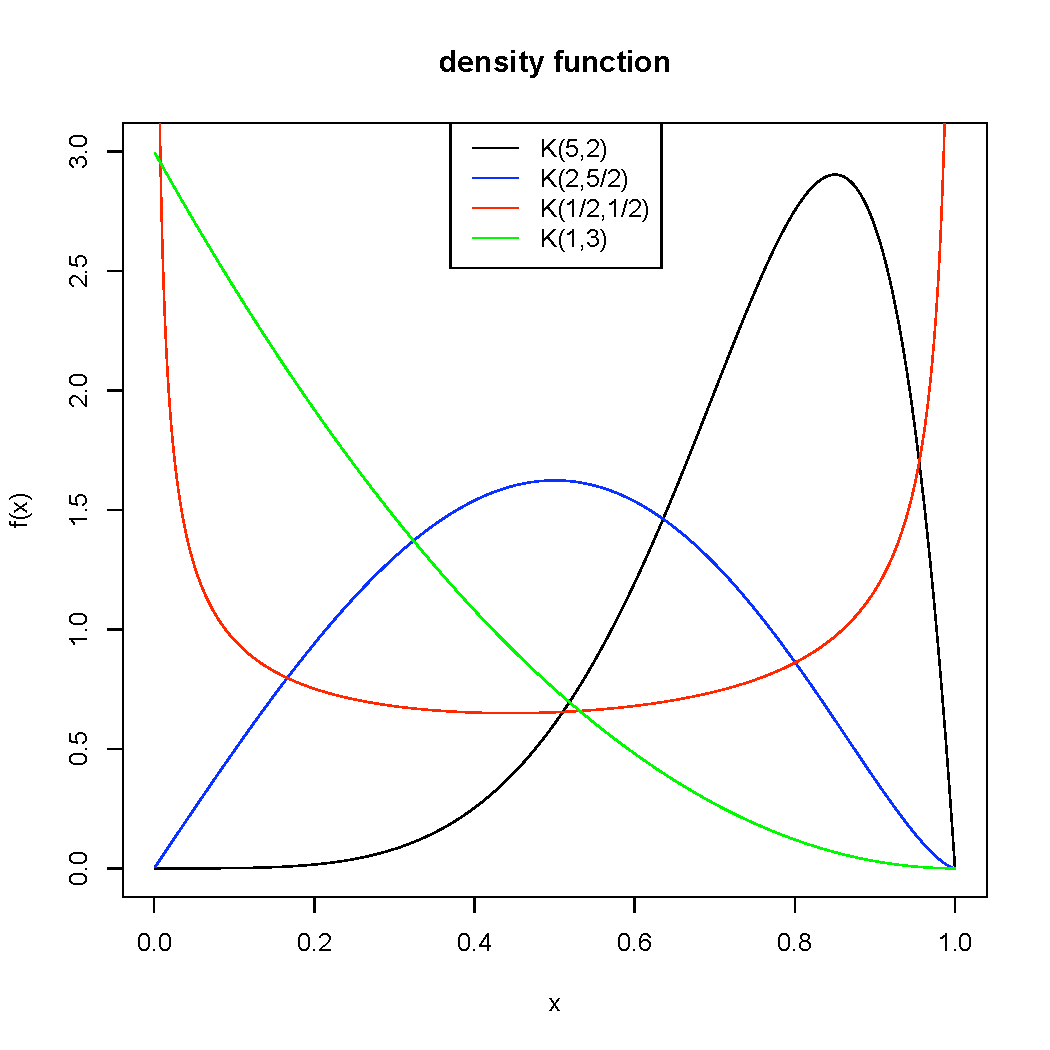
\includegraphics[width=0.48\textwidth]{img/kumarzoom}
  \end{center}
  \vspace{-20pt}  
  \caption{Density function for Kumaraswamy distributions}
\end{wrapfigure}
The Kumaraswamy distribution has the following density function
$$
f(x) = abx^{a-1}(1-x^a)^{b-1},
$$
where $x\in [0,1]$, $a,b>0$. Its distribution function is 
$$
F(x) = 1-(1-x^a)^b.
$$
A construction of the Kumaraswamy distribution use minimum/maximum of uniform samples. Let $n$
be the number of samples (each with $m$ i.i.d. uniform variate), then the distribution of the minimumm of all maxima (by sample) is a Kumaraswamy $\mcal Ku(m,n)$, which is also the distribution of one minus the maximum of all minima.

From \cite{jones}, the shapes of the density behaves as follows
\begin{itemize}
\item $a,b>1$ implies unimodal density,
\item $a>1, b\leq 1$ implies increasing density,
\item $a=b=1$ implies constant density,
\item $a\leq 1, b >1$ implies decreasing density,
\item $a,b<1$ implies uniantimodal,
\end{itemize}
which is examplified in the figure on the right.

\subsection{Properties}
Moments for a Kumaraswamy distribution are available and computable with
$$
E(X^\tau )= b\beta(1+\frac{\tau}{a},b)
$$
when $\tau > -a$ with $\beta(.,.)$ denotes the beta function. Thus the expectation of a Kumaraswamy distribution is $E(X)=\frac{b\Gamma(1+1/a)\Gamma(b)}{\Gamma(1+1/a+b)}$ and its variance $Var(X) = b\beta(1+\frac{2}{a},b) - b^2\beta^2(1+\frac{1}{a},b)$.

\subsection{Estimation}
From \cite{jones}, the maximum likelihood estimators are computable by the following procedure
\begin{enumerate}
\item solve the equation $\frac{n}{a}\left(1+\frac{1}{n}\sum_{i=1}^n \frac{\log Y_i}{1-Y_i} + \frac{ \sum_{i=1}^n \frac{Y_i\log Y_i}{1-Y_i} }{ \sum_{i=1}^n \log(1- Y_i) } \right)$ with $Y_i=X_i^a$ to find $\hat a$\footnote{the solution for this equation exists and is unique.},
\item compute $\hat b = -n\left( \sum_{i=1}^n \log(1- X_i^{\hat a}) \right)^{-1}$.
\end{enumerate}

\subsection{Random generation}
Since the quantile function is explicit
$$
F^{-1}(u) = \left(1-\left(1-u\right)^{\frac{1}{b}} \right)^{\frac{1}{a}},
$$
an inversion function method $F^{-1}(U)$ with $U$ uniformly distributed is easily computable.


\subsection{Applications}
From wikipedia, we know a good example of the use of the Kumaraswamy distribution: the storage volume of a reservoir of capacity $z_{max}$ whose upper bound is $z_{max}$ and lower bound is 0.

%----------------------------------------------------------------------------------------------------------
% 	Copyright (c) 2009 R-forge 'distributions' Core Team, 
% 	
%	The following Sweave code is under the GNU Free Documentation License:
%      	Permission is granted to copy, distribute and/or modify this document
%      	under the terms of the GNU Free Documentation License, Version 1.3
%      	or any later version published by the Free Software Foundation;
%      	with no Invariant Sections, no Front-Cover Texts, and no Back-Cover Texts.
%
%      A copy of the license is included in the 'inst' directory of this package 
%      or on the web at http://www.gnu.org/licenses/licenses.html#FDL
%
%	After running Sweave, the following code could be compiled :
%	  - on windows with a Tex distribution such as miktex (http://miktex.org) 
%		and a front end Latex editor such as texniccenter (http://www.toolscenter.org)
%	  - on mac os with a Tex distribution such as TexLive and a front end Latex
%	  	editor such as Texshop (http://www.uoregon.edu/~koch/texshop/)
%	  - on linux with a Tex distribution such as teTex (http://www.tug.org/teTeX/)
%	  	and a front end Latex editor such as emacs (http://www.gnu.org/software/emacs/)
%
%----------------------------------------------------------------------------------------------------------

\chapter{The Gaussian family}
%%%%%%%%%%%%%%%%%%%%%%%%%%%%%%%%%%%%%%%%%%%%%%%%%
\section{The Gaussian (or normal) distribution}


The normal distribution comes from the study of astronomical data by the German mathematician Gauss. That's why it is widely called the Gaussian distribution. But there are some hints to think that Laplace has also used this distribution. Thus sometimes we called it the Laplace Gauss distribution, a name introduced by K. Pearson who wants to avoid a querelle about its name.


\subsection{Characterization}
\begin{wrapfigure}{r}{0.5\textwidth}
  \begin{center}
    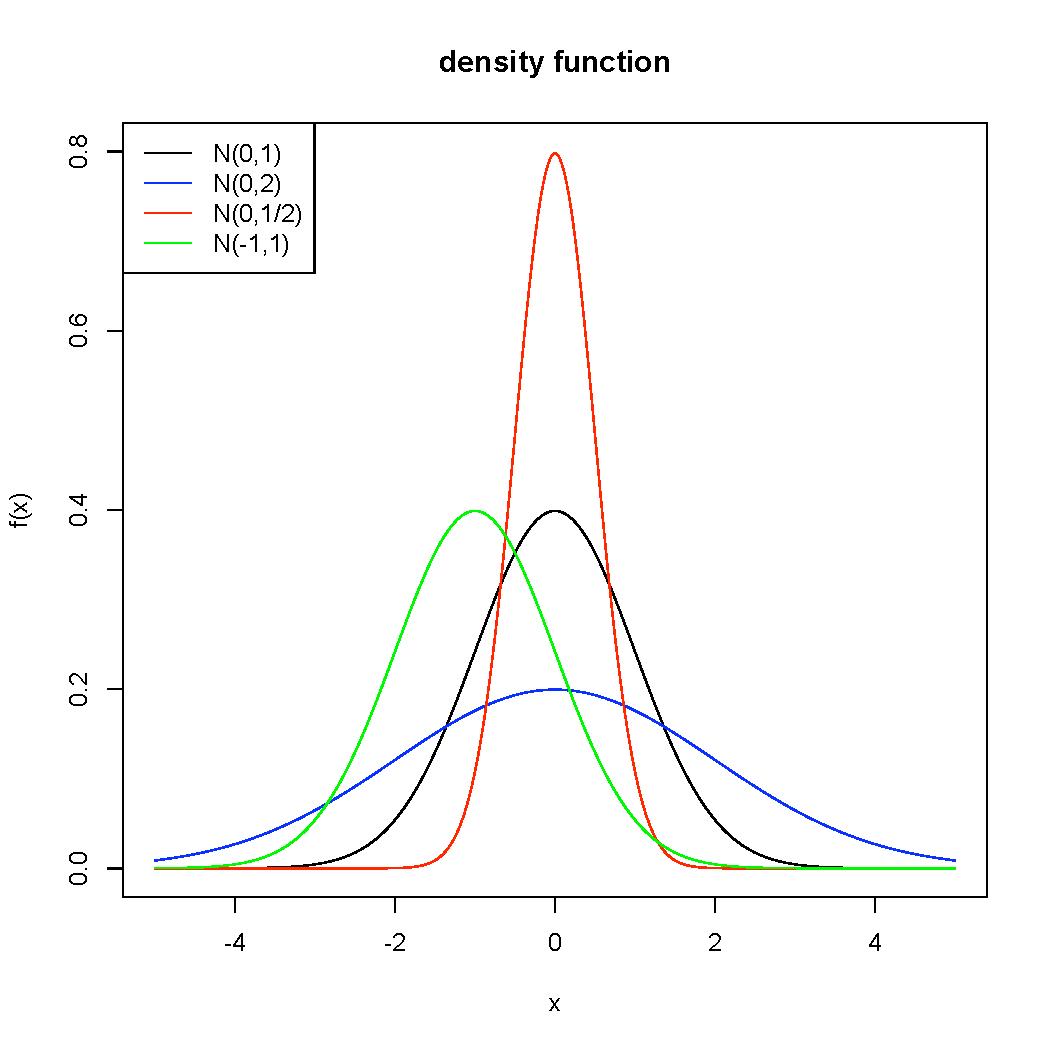
\includegraphics[width=0.48\textwidth]{img/normzoom}
  \end{center}
  \caption{The density of Gaussian distributions}
\end{wrapfigure}

The density of a normal distribution $\mathcal N(\mu, \sigma^2)$ is 
$$
f(x) =  \frac{1}{\sigma\sqrt{2\pi}} \,e^{ -\frac{(x- \mu)^2}{2\sigma^2}},
$$
where $x\in \mathbb R$ and $\mu (\in \mathbb R)$ denotes the mean of the distribution (a location parameter) and $\sigma^2 (>0)$ its variance (a scale parameter).



Its distribution function is then
$$
F(x) = \int_{-\infty}^x \frac{1}{\sigma\sqrt{2\pi}} \,e^{ -\frac{(x- \mu)^2}{2\sigma^2}} \,du,
$$
which has no explicit expressions. Many softwares have this distribution function implemented, since it is The basic distribution. Generally, we denote by $\Phi$ the distribution function a $\mathcal N(0, 1)$ normal distribution, called the standard normal distribution. $F$ can be rewritten as
$$
F(x) = \Phi\left(\frac{x-\mu}{\sigma}\right).
$$

Finally, the normal distribution can also be characterized through its moment generating function
$$
M(t) = e^{mt + \frac{\sigma^2t^2}{2}},
$$
as well as its characteristic function
$$
\phi(t) = e^{imt - \frac{\sigma^2t^2}{2}}.
$$

\subsection{Properties}
It is obvious, but let us recall that the expectation (and the median) of a normal distribution $ \mathcal N(\mu, \sigma^2)$ is $\mu$ and its variance $\sigma^2$. Furthermore if $X\sim \mathcal N(0, 1)$ we have that $E(X^n) = 0$ if $x$ is odd and $\frac{(2n)!}{2^n n!}$ if $x$ is even.



The biggest property of the normal distribution is the fact that the Gaussian belongs to the family of stable distribution (i.e. stable by linear combinations). Thus we have
\begin{itemize}
\item if $X\sim \mathcal N(\mu, \sigma^2)$ and $Y\sim \mathcal N(\nu, \rho^2)$, then $aX+bY\sim\mathcal N(a\mu+b\nu, a^2\sigma^2+b^2\rho^2+2abCov(X,Y))$, with the special case where $X,Y$ are independent cancelling the covariance term.
\item if $X\sim \mathcal N(\mu, \sigma^2)$, $a,b$ two reals, then $aX+b\sim \mathcal N(a\mu+b, a^2\sigma^2)$.
\end{itemize}

If we consider an i.i.d. sample of $n$ normal random variables $(X_i)_{1\leq i\leq n}$, then the sample mean $\overline X_n$ follows a $\mathcal N(\mu, \frac{\sigma^2}{n})$ independently from the sample variance $S^2_n$ such that $\frac{S_n^2 n}{\sigma^2}$ follows a chi-square distribution with $n-1$ degrees of freedom.

A widely used theorem using a normal distribution is the central limit theorem:\\
If $(X_i)_{1\leq i\leq n}$ are i.i.d. with mean $m$ and finite variance $s^2$, then
$\frac{\sum_{i=1}^n X_i - nm}{s\sqrt{n}} \stackrel{\mathcal L}{\longrightarrow} \mathcal N(0,1)$. If we drop the hypothesis of identical distribution, there is still an asymptotic convergence (cf. theorem of Lindeberg-Feller).


\subsection{Estimation}
The maximum likelihood estimators are 
\begin{itemize}
\item $ \overline X_n = \frac{1}{n} \sum_{i=1}^n X_i \sim \mathcal N(\mu, \frac{\sigma^2}{n})$ is the unbiased estimator with minimum variance of $\mu$,
\item $S^2_n = \frac{1}{n-1} \sum_{i=1}^n (X_i- \overline X_n)^2 \sim \chi_{n-1}^2$ is the unbiased estimator with minimum variance of $\sigma^2$\footnote{This estimator is not the maximum likelihood estimator since we unbias it.},
\item $\hat \sigma_n = \sqrt{\frac{n-1}{2}}\frac{\Gamma(\frac{n-1}{2})}{\Gamma(\frac{n}{2})} \sqrt{S_n^2}$ is the unbiased estimator with minimum variance of $\sigma$ but we generally use $\sqrt{S_n^2}$.
\end{itemize}

Confidence intervals for these estimators are also well known quantities
\begin{itemize}
\item $I(\mu) = \left[\overline X_n - \sqrt{\frac{S_n^2}{n}} t_{n-1,\alpha/2}; \overline X_n + \sqrt{\frac{S_n^2}{n}} t_{n-1,\alpha/2}\right]$,
\item $I(\sigma^2) = \left[\frac{S_n^2 n}{ z_{n-1,\alpha/2}}; \frac{S_n^2n}{ z_{n-1,1-\alpha/2}}\right]$,
\end{itemize}
where $t_{n-1,\alpha/2}$ and $z_{n-1,\alpha/2}$ are quantiles of the Student and the Chi-square distribution.

\subsection{Random generation}
The Box-Muller algorithm produces normal random variates:
\begin{itemize}
\item generate $U,V$ from a uniform $\mathcal U(0,1)$ distribution,
\item compute $X = \sqrt{-2\log U} \cos(2\pi V)$ and $Y = \sqrt{-2\log U} \sin(2\pi V)$.
\end{itemize}
In outputs, $X$ and $Y$ follow a standard normal distribution (independently).

But there appears that this algorithm under estimates the tail of the distribution (called the Neave effect, cf. \cite{patard}), most softwares use the inversion function method, consist in computing the quantile function $\Phi^{-1}$ of a uniform variate.

\subsection{Applications}
From wikipedia, here is a list of situations where approximate normality is sometimes assumed
\begin{itemize}
\item In counting problems (so the central limit theorem includes a discrete-to-continuum approximation) where reproductive random variables are involved, such as Binomial random variables, associated to yes/no questions or Poisson random variables, associated to rare events;
\item In physiological measurements of biological specimens: logarithm of measures of size of living tissue (length, height, skin area, weight) or length of inert appendages (hair, claws, nails, teeth) of biological specimens, in the direction of growth; presumably the thickness of tree bark also falls under this category or other physiological measures may be normally distributed, but there is no reason to expect that a priori;
\item Measurement errors are often assumed to be normally distributed, and any deviation from normality is considered something which should be explained;
\item Financial variables: changes in the logarithm of exchange rates, price indices, and stock market indices; these variables behave like compound interest, not like simple interest, and so are multiplicative; or  other financial variables may be normally distributed, but there is no reason to expect that a priori;
\item Light intensity: intensity of laser light is normally distributed or thermal light has a Bose-Einstein distribution on very short time scales, and a normal distribution on longer timescales due to the central limit theorem.
\end{itemize}

%%%%%%%%%%%%%%%%%%%%%%%%%%%%%%%%%%%%%%%%%%%%%%%
\section{Log normal distribution}
\subsection{Characterization}
\begin{wrapfigure}{r}{0.5\textwidth}
  \begin{center}
    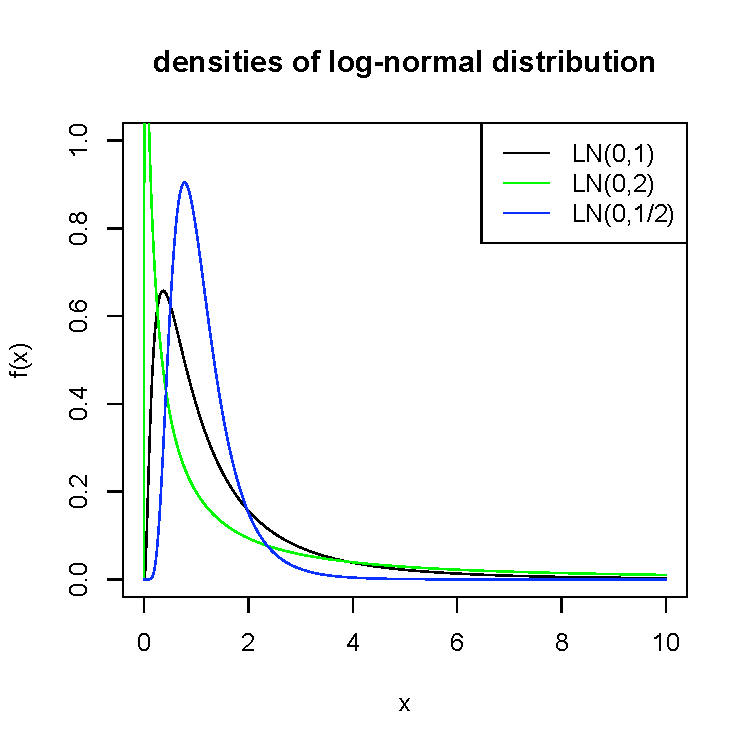
\includegraphics[width=0.48\textwidth]{img/lognormaldistrzoom}
  \end{center}
  \caption{The density of log-normal distributions}
\end{wrapfigure}

One way to characterize a random variable follows a log-normal distribution is to say that its logarithm is normally distributed. Thus the distribution function of a log-normal distribution ($\mathcal L \mathcal G(\mu,\sigma^2)$) is
$$
F(x) = \Phi\left(\frac{\log(x)-\mu}{\sigma}\right),
$$
where $\Phi$ denotes the distribution function of the standard normal distribution and $x>0$.

From this we can derive an explicit expression for the density $\mathcal L \mathcal G(\mu,\sigma^2)$
$$
f(x) =  \frac{1}{\sigma x \sqrt{2\pi}} \,e^{ -\frac{(\log(x)- \mu)^2}{2\sigma^2}},
$$
for $x>0$, $\mu\in\mathbb R$ and $\sigma^2 >0$.

A log-normal distribution does not have finite characteristic function or moment generating function.

\subsection{Properties}
The expectation and the variance of a log-normal distribution are $E(X) = e^{\mu+\frac{\sigma^2}{2}}$ and $Var(X) = (e^{\sigma^2}-1)e^{2\mu+\sigma^2}$. And raw moments are given by $E(X^n) = e^{n\mu + \frac{n^2\sigma^2}{2}}$. The median of a log-normal distribution is $e^\mu$.

From \cite{klugman}, we also have a formula for limited expected values
$$
E\left((X\wedge L)^k\right) = e^{k(\mu+\frac{k\sigma^2}{2}} \Phi(u-k\sigma) + L^k (1- \Phi(u)),
$$
where $u=\frac{\log(L)-\mu}{\sigma}$.

Since the Gaussian distribution is stable by linear combination, log-normal distribution is stable by product combination. That is to say if we consider $X$ and $Y$ two independent log-normal variables ($\mathcal L \mathcal G(\mu,\sigma^2)$ and $\mathcal L \mathcal G(\nu,\rho^2)$),
we have $XY$ follows a log-normal distribution $\mathcal L \mathcal G(\mu+\nu,\sigma^2+\rho^2)$.
Let us note that $\frac{X}{Y}$ also follows a log-normal distribution $\mathcal L \mathcal G(\mu-\nu,\sigma^2+\rho^2)$.

An equivalence of the Limit Central Theorem for the log-normal distribution is the product of i.i.d. random variables $(X_i)_{1\leq i\leq n}$ asymptotically follows a log-normal distribution with paramter $n E(\log(X))$ and $n Var(\log(X))$.

\subsection{Estimation}
Maximum likelihood estimators for $\mu$ and $\sigma^2$ are simply
\begin{itemize}
\item $\hat \mu = \frac{1}{n} \sum_{i=1}^n\log(x_i)$ is an unbiased estimator of $\mu$,
\item $\widehat{\sigma^2} = \frac{1}{n-1} \sum_{i=1}^n (\log(x_i)- \hat \mu)^2$ is an unbiased estimator of $\sigma^2$\footnote{As for the $\sigma^2$ estimator of normal distribution, this estimator is not the maximum likelihood estimator since we unbias it.}.
\end{itemize}
One amazing fact about parameter estimations of log-normal distribution is that those estimators are very stable. 

\subsection{Random generation}
Once we have generated a normal variate, it is easy to generate a log-normal variate just by taking the exponential of normal variates.

\subsection{Applications}
There are many applications of the log-normal distribution. \cite{logappli} focuses on application of the log-normal distribution. For instance, in finance the Black \& Scholes assumes that assets are log-normally distributed (cf. \cite{blackscholes73} and the extraordinary number of articles citing this article).
\cite{biolognorm} deals with environmental applications of the log-normal distribution.



%%%%%%%%%%%%%%%%%%%%%%%%%%%%%%%%%%%%%%%%%%%%%%%
\newpage\section{Shifted log normal distribution}
\subsection{Characterization}
\begin{wrapfigure}{r}{0.5\textwidth}
  \vspace{-20pt}
  \begin{center}
    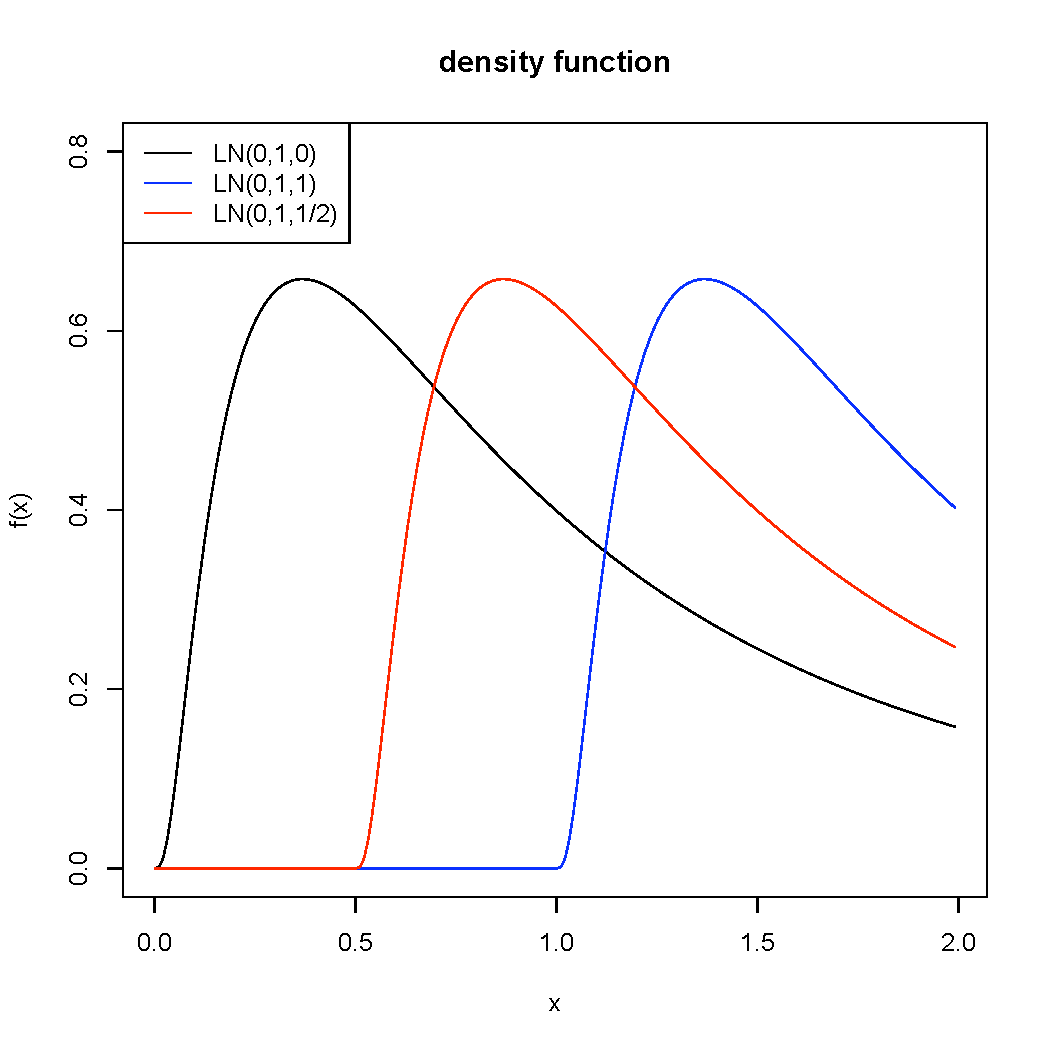
\includegraphics[width=0.48\textwidth]{img/shiftlognormzoom}
  \end{center}
  \vspace{-20pt}
  \caption{The density of shifted log-normal distributions}
  \vspace{-20pt}
\end{wrapfigure}
An extension to the log-normal distribution is the translated log-normal distribution. It is
the distribution of $X+\nu$ where $X$ follows a log-normal distribution.
It is characterized by the following distribution function
$$
F(x) = \Phi\left(\frac{\log(x-\nu)-\mu}{\sigma}\right),
$$
where $\Phi$ denotes the distribution function of the standard normal distribution and $x>0$.
Then we have this expression for the density $\mathcal T\mathcal L \mathcal G(\nu,\mu,\sigma^2)$
$$
f(x) =  \frac{1}{\sigma (x-\nu) \sqrt{2\pi}} \,e^{ -\frac{(\log(x-\nu)- \mu)^2}{2\sigma^2}},
$$
for $x>0$, $\mu,\nu\in\mathbb R$ and $\sigma^2 >0$.

As for the log-normal distribution, there is no moment generating function nor characteristic function.

\subsection{Properties}
The expectation and the variance of a log-normal distribution are $E(X) =\nu+ e^{\mu+\frac{\sigma^2}{2}}$ and $Var(X) = (e^{\sigma^2}-1)e^{2\mu+\sigma^2}$. And raw moments are given by $E(X^n) = e^{n\mu + \frac{n^2\sigma^2}{2}}$. 

\subsection{Estimation}
An intuitive approach is to estimate $\nu$ with $X_{1:n}$, then estimate parameters on shifted samples $(X_i-\nu)_i$.

\subsection{Random generation}
Once we have generated a normal variate, it is easy to generate a log-normal variate just by taking the exponential of normal variates and adding the shifted parameter $\nu$.

\subsection{Applications}
An application of the shifted log-normal distribution to finance can be found in \cite{haahtela} or
\cite{brigo}.

%%%%%%%%%%%%%%%%%%%%%%%%%%%%%%%%%%%%%%%%%%%%%%
\section{Inverse Gaussian distribution}
\subsection{Characterization}

\begin{wrapfigure}{r}{0.5\textwidth}
  \vspace{-30pt}
  \begin{center}
    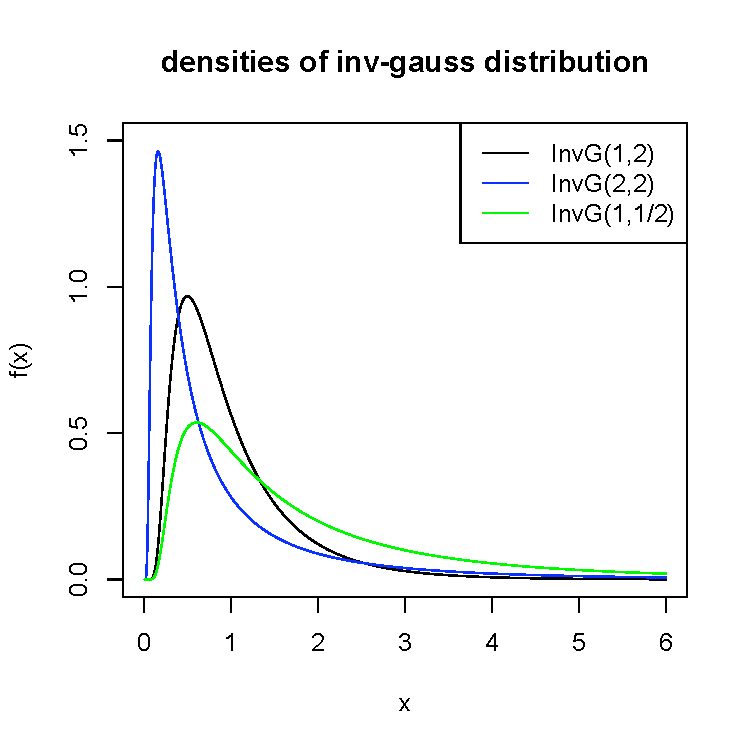
\includegraphics[width=0.48\textwidth]{img/invgaussdistrzoom}
  \end{center}
  \vspace{-20pt}
  \caption{The density of inverse Gaussian distributions}
  \vspace{-20pt}
\end{wrapfigure}

The density of an inverse Gaussian distribution $\mathcal I \mathcal G(\nu, \lambda)$ is given by
$$
f(x)=\sqrt{\frac{\lambda}{2\pi x^3}}\exp\left[-\lambda\frac{(x-\nu)^2}{2\nu^2 x}\right],
$$
while its distribution function is
$$
F(x)=\Phi\left[\sqrt{\frac{\lambda}{x}}\left(\frac{x}{\nu}-1\right)\right]+e^{2\lambda/\nu}\Phi\left[\sqrt{\frac{\lambda}{x}}\left(\frac{x}{\nu}+1\right)\right],
$$
for $x>0$, $\nu\in\mathbb R$, $\lambda>0$ and $\Phi$ denotes the usual standard normal distribution.

Its characteristic function is 
$$
\phi(t) = e^{\left(\frac{\lambda}{\nu}\right)\left[1-\sqrt{1-\frac{2\nu^2\mathrm{i}t}{\lambda}}\right]}.
$$

The moment generating function is expressed as
$$
M(t) = e^{\left(\frac{\lambda}{\nu}\right)\left[1-\sqrt{1-\frac{2\nu^2t}{\lambda}}\right]}.
$$

\subsection{Properties}
The expectation of an inverse Gaussian distribution $\mathcal I \mathcal G(\nu, \lambda)$ is
$\nu$ and its variance $\frac{\nu^3}{\lambda}$.

Moments for the inverse Gaussian distribution are given 
$E(X^n) = \nu^n \sum_{i=0}^{n-1}\frac{\Gamma(n+i)}{\Gamma(i+1)\Gamma(n-i)} (\frac{2\lambda}{\nu})^i$ for $n$ integer.

From \cite{yu}, we have the following properties
\begin{itemize}
\item if $X$ is inverse Gaussian distributed $\mcal I \mcal G(\nu, \lambda)$, then $aX$ follows an inverse Gaussian distribution $\mcal I \mcal G(a\nu, a\lambda)$ for $a>0$
\item if $(X_i)_i$ are i.i.d. inverse Gaussian variables, then the sum $\sum_{i=1}^n X_i$ still follows an inverse Gaussian distribution $\mcal I \mcal G(n\nu, n^2\lambda)$
\end{itemize}


\subsection{Estimation}
Maximum likelihood estimators of $\nu$ and $\lambda$ are
$$
\hat{\mu}= \bar X_n
\txtm{and} 
\hat{\lambda}= n \left( \sum_{i=1}^n \left( \frac1{X_i}-\frac1{\hat{\mu}} \right) \right)^{-1}.
$$
From previous properties, $\hat \mu$ follows an inverse gaussian distribution $\mcal I\mcal G(\mu,n\lambda)$ and $\frac{n\lambda}{\hat \lambda}$ follows a chi-squared distribution $\chi_{n-1}^2$.


\subsection{Random generation}
NEED 	

Mitchael,J.R., Schucany, W.R. and Haas, R.W. (1976). Generating
	random roots from variates using transformations with multiple roots.
	American Statistician. 30-2. 88-91.

\subsection{Applications}
NEED REFERENCE

%%%%%%%%%%%%%%%%%%%%%%%%%%%%%%%%%%%%%%%%%%%%%%%%%
\section{The generalized inverse Gaussian distribution} \label{sec:gig}
This section is taken from \cite{ghyp}.

\subsection{Characterization}
\begin{wrapfigure}{r}{0.5\textwidth}
  \vspace{-60pt}
  \begin{center}
    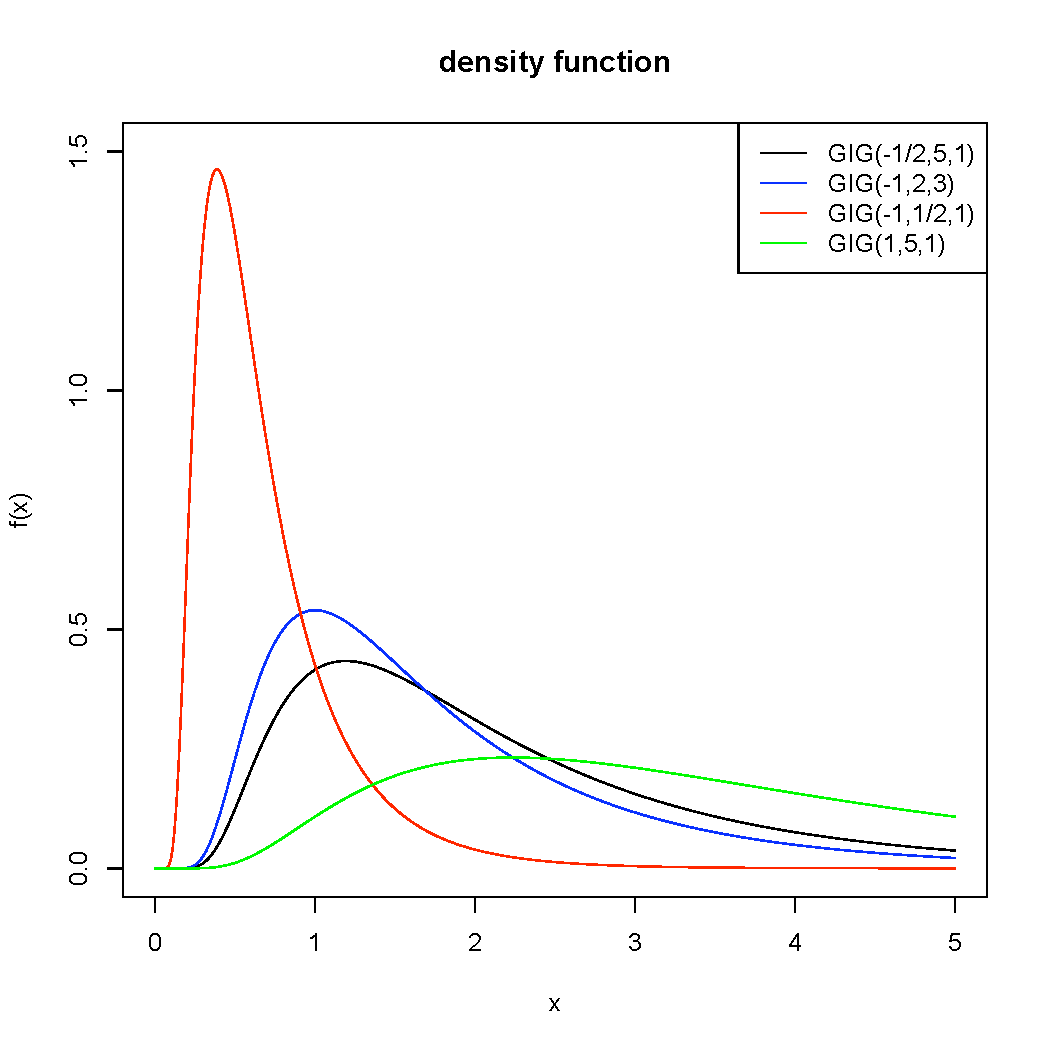
\includegraphics[width=0.48\textwidth]{img/gigzoom}
  \end{center}
  \vspace{-20pt}
  \caption{The density of generalized inverse Gaussian distributions}
  \vspace{-20pt}
\end{wrapfigure}
A generalization of the inverse Gaussian distribution exists but there is no
closed form for its distribution function and its density used Bessel functions.
The latter is as follows
$$\label{eq:densgig}
 f(x) = \left(\frac{\psi}{\chi}\right)^{\frac{\lambda}{2}}
  \frac{x^{\lambda-1}}{2K_\lambda(\sqrt{\chi\psi})} \,
  \exp\left\{-\frac{1}{2}\left(\frac{\chi}{x}+\psi x
    \right)\right\},
$$
where $x>0$ and $K_\lambda$ denotes the modified Bessel function. Parameters must satisfy
\begin{itemize}
\item $\chi > 0, \psi \geq 0$, when $\lambda < 0 $,
\item $\chi > 0, \psi > 0$, when $\lambda = 0$,
\item $\chi \geq 0, \psi > 0$, when $\lambda > 0 $.
\end{itemize} 
The generalized inverse Gaussian is noted as $\mathcal G \mathcal I \mathcal G(\lambda,\psi,\chi)$.

Closed form for distribution function??

Plot

The moment generating function is given by
\begin{equation}
  M(t) = \left(\frac{\psi}{\psi - 2 t}\right)^{\lambda / 2}
  \frac{K_\lambda(\sqrt{\chi (\psi - 2 t)})}{K_\lambda(\sqrt{\chi \psi})}.
\end{equation}


\subsection{Properties}
The expectation is given by 
$$
\sqrt{\frac{\chi}{\psi}}
  \frac{K_{\lambda+1}(\sqrt{\chi\psi})}{K_{\lambda}(\sqrt{\chi\psi})},
$$ and more generally the $n$-th moment is as follows
$$
  E(X^n) = \left(\frac{\chi}{\psi}\right)^\frac{n}{2}
  \frac{K_{\lambda+n}(\sqrt{\chi\psi})}{K_\lambda(\sqrt{\chi\psi})}.
$$
Thus we have the following variance
$$
Var(X) = \frac{\chi}{\psi}
  \frac{K_{\lambda+2}(\sqrt{\chi\psi})}{K_\lambda(\sqrt{\chi\psi})} - \frac{\chi}{\psi}
  \left(\frac{K_{\lambda+1}(\sqrt{\chi\psi})}{K_\lambda(\sqrt{\chi\psi})}\right)^2.
$$


Furthermore,
\begin{equation}\label{eq:eloggig}
  E(\log X) =  \frac{\partial d E(X^\alpha)}{\partial d \alpha}\biggr|_{\alpha=0}.
\end{equation}
Note that numerical calculations of $E(\log X)$ may be performed
with the integral representation as well.



\subsection{Estimation}
NEED REFERENCE

\subsection{Random generation}
NEED REFERENCE


 
\chapter{Exponential distribution and its extensions}
%%%%%%%%%%%%%%%%%%%%%%%%%%%%%%%%%%%%%%%%%%%%%%%
\section{Exponential distribution}
\subsection{Characterization}
\begin{wrapfigure}{r}{0.5\textwidth}
  \vspace{-20pt}
  \begin{center}
    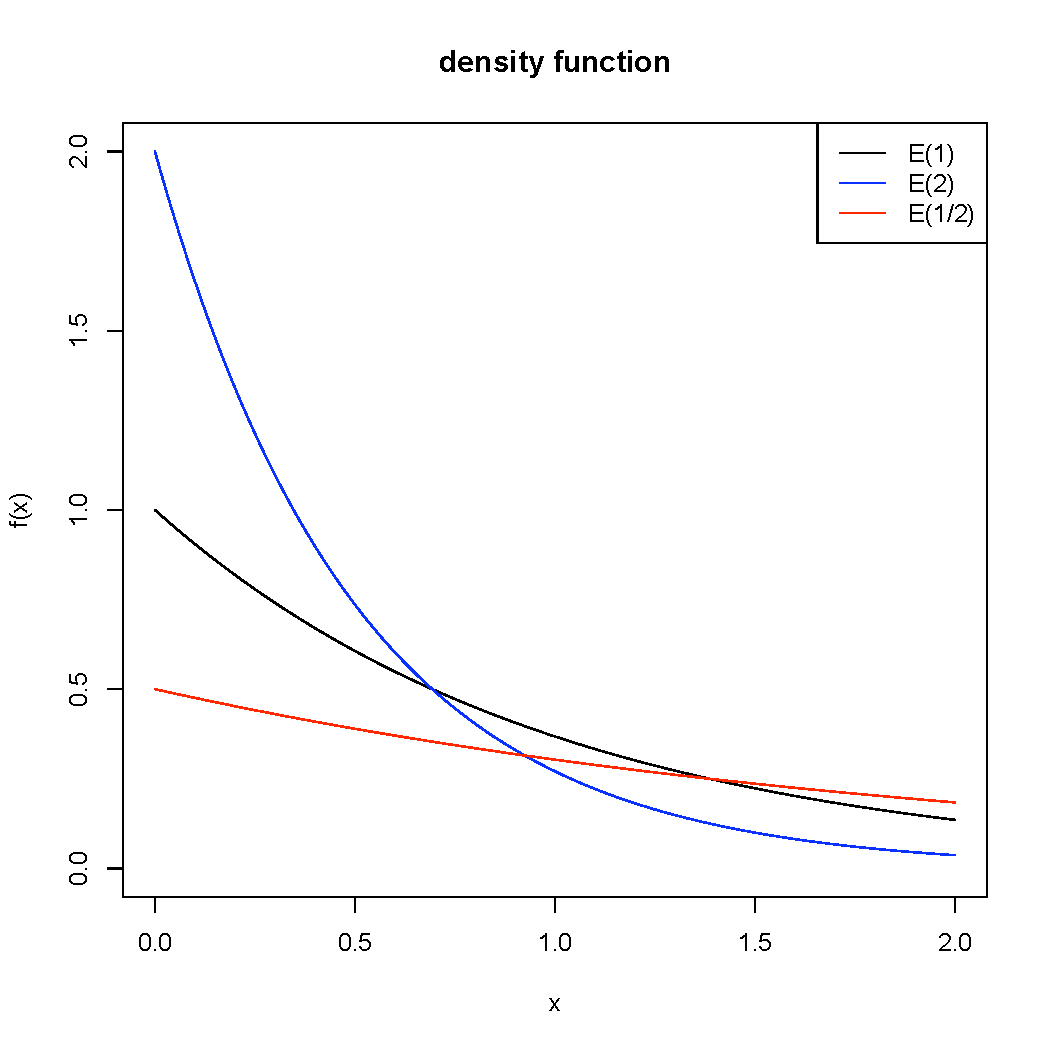
\includegraphics[width=0.48\textwidth]{img/expzoom}
  \end{center}
  \vspace{-20pt}  
  \caption{Density function for exponential distributions}
%  \vspace{-20pt}  
\end{wrapfigure}

The exponential is a widely used and widely known distribution. It is characterized
by the following density
$$
f(x) = \lambda e^{-\lambda x},
$$
for $x>0$ and $\lambda >0$. Its distribution function is
$$
F(x) =  1-e^{-\lambda x}.
$$

Since it is a light-tailed distribution, the moment generating function of an exponential distribution 
$\mathcal E(\lambda)$ exists which is
$$
M(t)=\frac{\lambda}{\lambda -t},
$$
while its characteristic function is 
$$
\phi(t) = \frac{\lambda}{\lambda-it}.
$$

\subsection{Properties}
The expectation and the variance of an exponential distribution $\mathcal E(\lambda)$
are $\frac{1}{\lambda}$ and $\frac{1}{\lambda^2}$. Furthermore the $n$-th moment is given
by 
$$
E(X^n) = \frac{\Gamma(n+1)}{\lambda^n}.
$$

The exponential distribution is the only one continuous distribution to verify the lack of memory property. That is to say if $X$ is exponentially distributed, we have
$$
\frac{P(X>t+s)}{P(X>s)} = P(X>t),
$$
where $t,s>0$.

If we sum $n$ i.i.d. exponentially distributed random variables, we get a gamma distribution $\mathcal G(n,\lambda)$.

\subsection{Estimation}
The maximum likelihood estimator and the moment based estimator are the same
$$
\hat \lambda = \frac{n}{\sum_{i=1}^n X_i} = \frac{1}{\overline X_n},
$$
for a sample $(X_i)_{1\leq i\leq n}$. But the unbiased estimator with mininum variance
is 
$$
\tilde \lambda  = \frac{n-1}{\sum_{i=1}^n X_i}.
$$
Exact confidence interval for parameter $\lambda$ is given by 
$$
I_\alpha(\lambda) = \left[ \frac{z_{2n,1-\frac{\alpha}{2}} }{2\sum_{i=1}^n X_i} , \frac{z_{2n,\frac{\alpha}{2}} }{2\sum_{i=1}^n X_i} \right],
$$
where $z_{n,\alpha}$ denotes the $\alpha$ quantile of the chi-squared distribution.

\subsection{Random generation}
Despite the quantile function is $F^{-1}(u)=-\frac{1}{\lambda}\log(1-u)$, generally the exponential distribution $\mathcal E(\lambda)$ is generated by applying $-\frac{1}{\lambda}\log(U)$ on 
a uniform variate $U$.

\subsection{Applications}
From wikipedia, the exponential distribution occurs naturally when describing the lengths of the inter-arrival times in a homogeneous Poisson process.

The exponential distribution may be viewed as a continuous counterpart of the geometric distribution, which describes the number of Bernoulli trials necessary for a ''discrete'' process to change state. In contrast, the exponential distribution describes the time for a continuous process to change state.

In real-world scenarios, the assumption of a constant rate (or probability per unit time) is rarely satisfied. For example, the rate of incoming phone calls differs according to the time of day. But if we focus on a time interval during which the rate is roughly constant, such as from 2 to 4 p.m. during work days, the exponential distribution can be used as a good approximate model for the time until the next phone call arrives. Similar caveats apply to the following examples which yield approximately exponentially distributed variables:
\begin{itemize}
\item the time until a radioactive particle decays, or the time between beeps of a geiger counter;
\item the time it takes before your next telephone call
\item the time until default (on payment to company debt holders) in reduced form credit risk modeling
\end{itemize}

Exponential variables can also be used to model situations where certain events occur with a constant probability per unit ''distance'':
\begin{itemize}
\item the distance between mutations on a DNA strand;
\item the distance between roadkill on a given road;
\end{itemize}

In queuing theory, the service times of agents in a system (e.g. how long it takes for a bank teller etc. to serve a customer) are often modeled as exponentially distributed variables.  (The inter-arrival of customers for instance in a system is typically modeled by the Poisson distribution in most management science textbooks.)  The length of a process that can be thought of as a sequence of several independent tasks is better modeled by a variable following the Erlang distribution (which is the distribution of the sum of several independent exponentially distributed variables).

Reliability theory and reliability engineering also make extensive use of the exponential distribution. Because of the ``memoryless'' property of this distribution, it is well-suited to model the constant hazard rate portion of the bathtub curve used in reliability theory. It is also very convenient because it is so easy to add failure rates in a reliability model.
The exponential distribution is however not appropriate to model the overall lifetime of organisms or technical devices, because the ``failure rates'' here are not constant: more failures occur for very young and for very old systems.

In physics, if you observe a gas at a fixed temperature and pressure in a uniform gravitational field, the heights of the various molecules also follow an approximate exponential distribution. This is a consequence of the entropy property mentioned below.


%%%%%%%%%%%%%%%%%%%%%%%%%%%%%%%%%%%%%%%%%%%%%%%
\newpage
\section{Shifted exponential}
\subsection{Characterization}
\begin{wrapfigure}{r}{0.5\textwidth}
  \vspace{-20pt}
  \begin{center}
    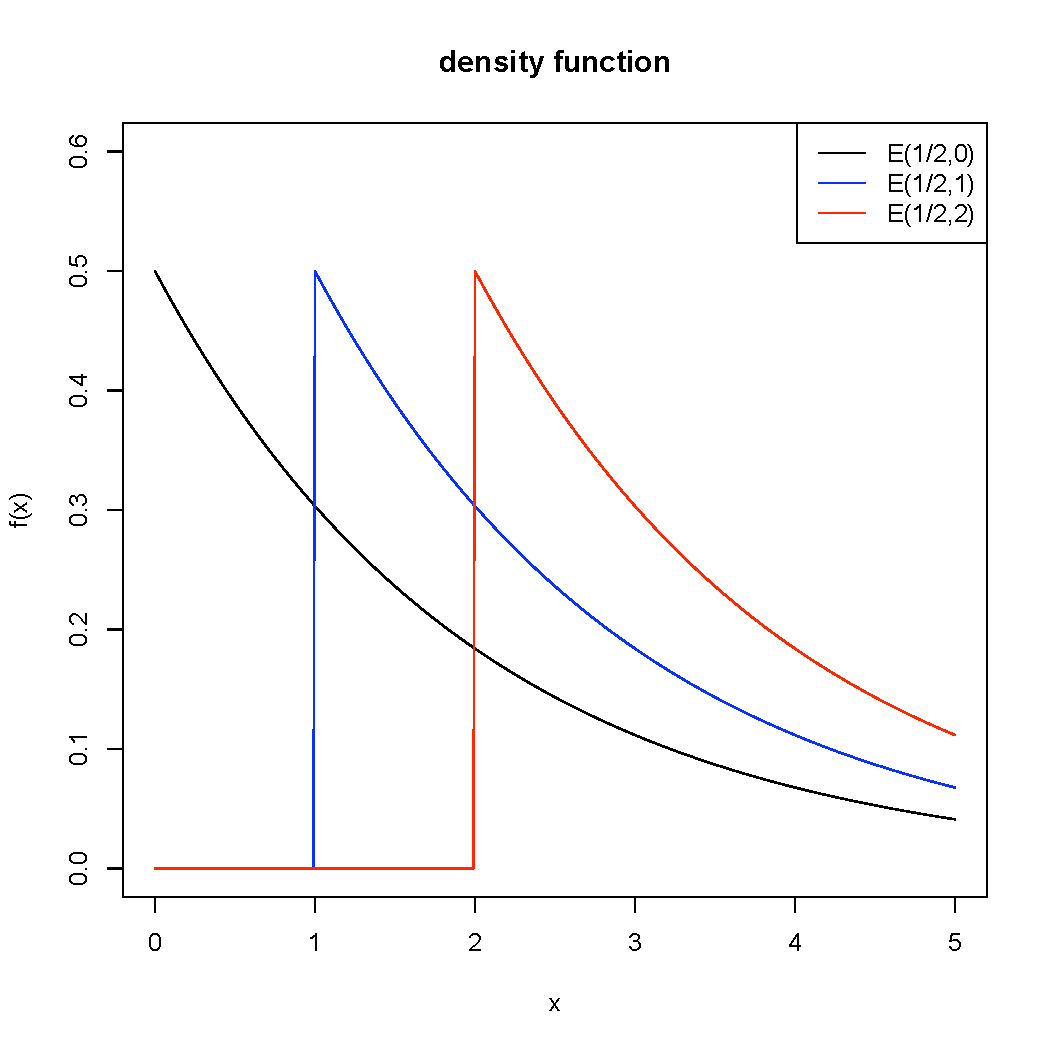
\includegraphics[width=0.48\textwidth]{img/shiftexpzoom}
  \end{center}
  \vspace{-20pt}  
  \caption{Density function for shifted exponential distributions}
\end{wrapfigure}
The distribution of the shifted exponential distribution is simply the distribution of $X-\tau$ when $X$ is exponentially distributed. Therefore the density is given by
$$
f(x) = \lambda e^{-\lambda(x-\tau)}
$$
for $x>\tau$.
The distribution function is given by
$$
F(x) = 1-e^{-\lambda(x-\tau)}
$$
for $x>\tau$.

As for the exponential distribution, there exists a moment generating function
$$
M(t) = e^{-t\tau} \frac{\lambda}{\lambda-t}
$$
and also a characteristic function
$$
\phi(t) = e^{-it\tau} \frac{\lambda}{\lambda-it}.
$$

\subsection{Properties}
The expectation and the variance of an exponential distribution $\mathcal E(\lambda,\tau)$
are $\tau+\frac{1}{\lambda}$ and $\frac{1}{\lambda^2}$. 

Furthermore the $n$-th moment (for $n$ integer) is computable with the binomial formula by 
$$
E(X^n) = \sum_{i=0}^n \frac{n!}{(n-i)!} \frac{(-\tau)^n}{(-\lambda\tau)^i}.
$$

\subsection{Estimation}
Maximum likelihood estimator for $\tau$ and $\lambda$ are given by
$$
\hat \tau = X_{1:n}
\txtm{and}
\hat \lambda = \frac{n}{\sum_{i=1}^n(X_i-\hat \tau)}
$$
where $X_{i:n}$ denotes the $i$th order statistic. Since the minimum $X_{1:n}$ follows a shifted exponential distribution $\mcal E(n\lambda,\tau)$, we have $\hat \tau$ is biased but asympotically unbiased.

NEED REFERENCE for unbiased estimators

\subsection{Random generation}
The random generation is simple: just add $\tau$ to the algorithm of exponential distribution.

\subsection{Applications}
NEED REFERENCE

%%%%%%%%%%%%%%%%%%%%%%%%%%%%%%%%%%%%%%%%%%%%%%%
\section{Inverse exponential}
\subsection{Characterization}
\begin{wrapfigure}{r}{0.5\textwidth}
  \vspace{-20pt}
  \begin{center}
    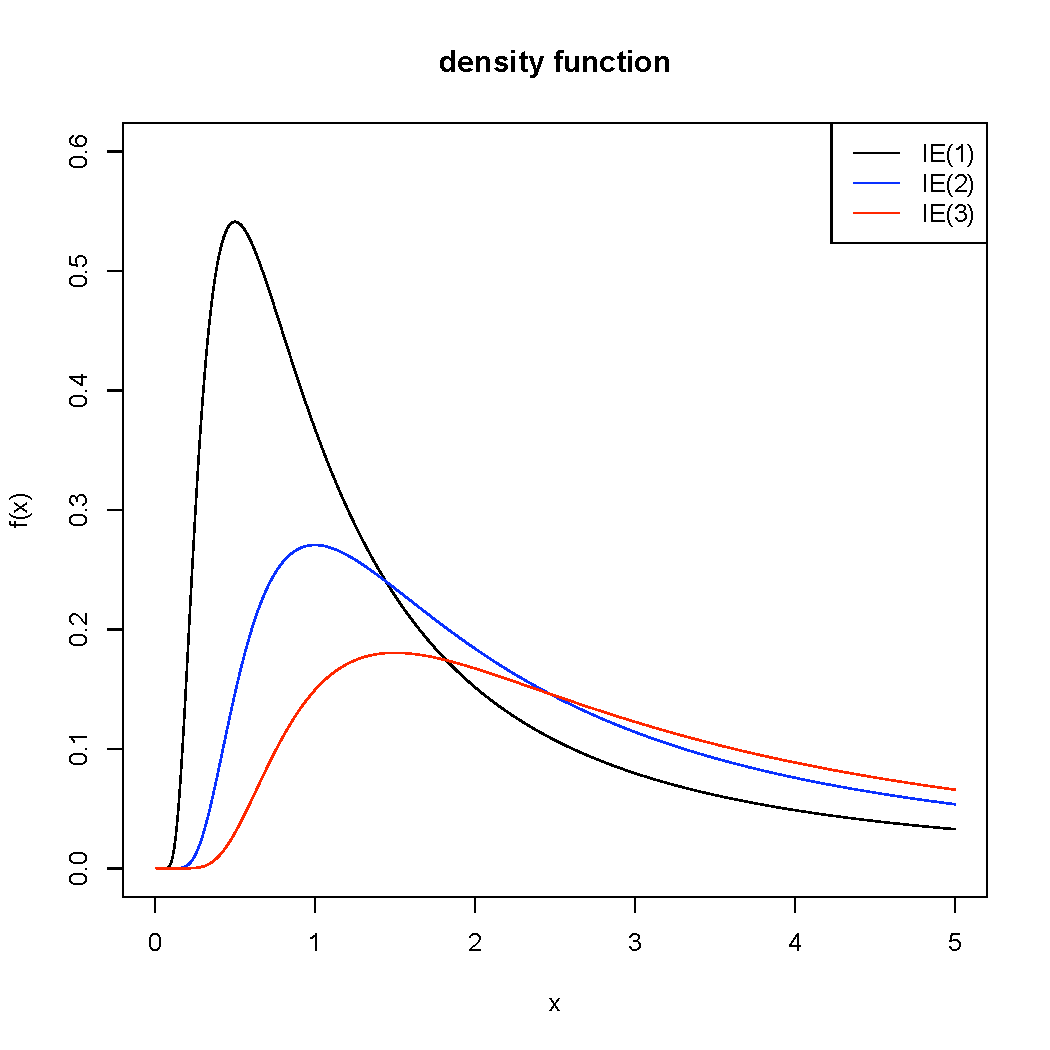
\includegraphics[width=0.48\textwidth]{img/invexpzoom}
  \end{center}
  \vspace{-20pt}  
  \caption{Density function for inverse exponential distributions}
\end{wrapfigure}
This is the distribution of the random variable $\frac{1}{X}$ when $X$ is exponentially distributed. The density defined as
$$
f(x)=\frac{\lambda}{x^2}e^{-\frac{\lambda}{x}},
$$
where $x>0$ and $\lambda>0$. The distribution function can then be derived as 
$$
F(x) =e^{-\frac{\lambda}{x}}.
$$
We can define inverse exponential distributions with characteristic or moment generating functions
$$
\phi(t)=2\sqrt{-it\lambda} K_1\left(2\sqrt{-i \lambda t}\right)
$$
and
$$
M(t)=2\sqrt{-it \lambda} K_1\left(2\sqrt{-\lambda t}\right).
$$
where $K_.(.)$ denotes the modified Bessel function.


\subsection{Properties}
Moments of the inverse exponential distribution are given by
$$
E(X^r) = \lambda^r * \Gamma(1-r)
$$
for $r <1$. Thus the expectation and the variance of the inverse exponential distribution do not exist.

\subsection{Estimation}
Maximum likelihood estimator of $\lambda$ is
$$
\hat \lambda = n \left(\sum_{i=1}^n\frac{1}{X_i} \right)^{-1},
$$
which is also the moment based estimator with $E(X^{-1}) = \lambda^{-1}$.

\subsection{Random generation}
The algorithm is simply to inverse an exponential variate of parameter $\frac{1}{\lambda}$, i.e. $(-\lambda \log(U))^{-1}$ for an uniform variable $U$.

\subsection{Applications}
NEED REFERENCE

%%%%%%%%%%%%%%%%%%%%%%%%%%%%%%%%%%%%%%%%%%%%%%%
\section{Gamma distribution}
\subsection{Characterization}
\begin{wrapfigure}{r}{0.5\textwidth}
  \vspace{-20pt}
  \begin{center}
    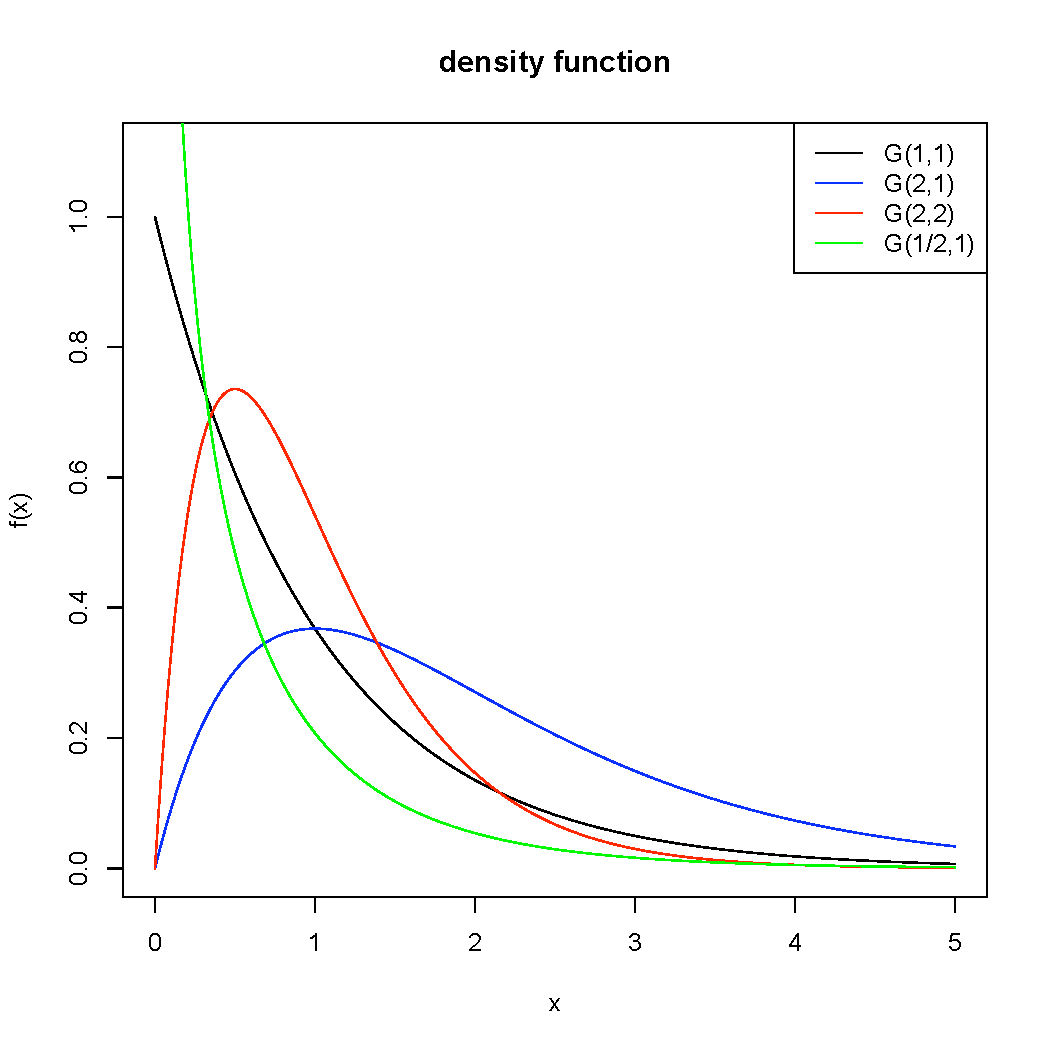
\includegraphics[width=0.48\textwidth]{img/gammazoom}
  \end{center}
  \vspace{-20pt}  
  \caption{Density function for gamma distributions}
\end{wrapfigure}

The gamma distribution is a generalization of the exponential distribution. Its density is defined as
$$
f(x)=\frac{\lambda^{\alpha}}{\Gamma(\alpha)} e^{-\lambda x} x^{\alpha-1},
$$
where $x\geq0$, $\alpha,\lambda>0$ and $\Gamma$ denotes the gamma function. We retrieve the exponential distribution by setting $\alpha$ to 1. When $\alpha$ is an integer, the gamma distribution is sometimes called the Erlang distribution.

The distribution function can be expressed in terms of the incomplete gamma distribution. We get
$$
F(x) = \frac{\gamma(\alpha,\lambda x)}{\Gamma(\alpha)},
$$
where $\gamma(.,.)$ is the incomplete gamma function. 

There is no analytical formula except when we deal with Erlang distribution (i.e. $\alpha \in \mathbb N$). In this case, we have
$$
F(x) = 1-\sum\limits_{i=0}^{\alpha-1} \frac{(\lambda x )^i}{i!}e^{-\lambda x} .
$$

For the gamma distribution, the moment generating and characteristic functions exist.
$$
\phi(t) = \left(\frac{\lambda}{\lambda-it}\right)^{-\alpha},
$$
and
$$
M(t) =\left(\frac{\lambda}{\lambda-t}\right)^{-\alpha}.
$$

\subsection{Properties}
The expectation of a gamma distribution $\mathcal G(\alpha, \lambda)$ is $E(X) = \frac{\alpha}{\lambda}$, while its variance is $Var(X) = \frac{\alpha}{\lambda^2}$. 

For a gamma distribution $\mcal G(\alpha, \lambda)$, the $\tau$th moment is given by
$$
E(X^r) =\lambda^r\frac{\Gamma(\alpha+r)}{\Gamma(\alpha)},
$$
provided that $\alpha+r>0$.

As for the exponential, we have a property on the convolution of gamma distributions. Let $X$ and $Y$ be gamma distributed $\mathcal G(\alpha,\lambda)$ and $\mathcal G(\beta,\lambda)$, we can prove that $X+Y$ follows a gamma distribution $\mathcal G(\alpha+\beta,\lambda)$.

For $X$ and $Y$ gamma distributed ($\mathcal G(\alpha,\lambda)$ and $\mathcal G(\beta,\lambda)$ resp.), we also have that $\frac{X}{X+Y}$ follows a beta distribution of the first kind with parameter $\alpha$ and $\beta$.

\subsection{Estimation}
Method of moments give the following estimators
$$
\tilde \alpha = \frac{(\bar X_n)^2}{S_n^2}
\txtm{and}
\tilde \lambda = \frac{\bar X_n}{S_n^2}.
$$
with $\bar X_n$ and $S_n^2$ the sample mean and variance.

Maximum likelihood estimators of $\alpha,\lambda$ verify the system
$$
\left\{
\begin{array}{l}
\log \alpha- \psi(\alpha)=    \log(\frac{1}{n}\sum_{i=1}^n X_i) -\frac{1}{n}\sum_{i=1}^n \log X_i \\
\lambda =\frac{n\alpha}{\sum_{i=1}^n X_i}\\
\end{array}
\right. ,
$$
where $\psi(.)$ denotes the digamma function. The first equation can be solved numerically\footnote{algorithm can be initialized with $\tilde \alpha$.} to get $\hat \alpha$ and then $\hat \lambda = \frac{\hat \alpha}{\bar X_n}$. But $\hat \lambda$ is biased, so the unbiased estimator with minimum variance of $\lambda$ is 
$$
\bar \lambda = \frac{\hat \alpha n}{\hat \alpha n -1}\frac{\hat \alpha}{\bar X_n}
$$

NEED REFERENCE for confidence interval

\subsection{Random generation}
Simulate a gamma $\mcal G(\alpha, \lambda)$ is quite tricky for non integer shape parameter. Indeed, if the shape parameter $\alpha$ is integer, then we simply sum $\alpha$ exponential random variables $\mcal E(\lambda)$. Otherwise we need to add a gamma variable $\mcal G(\alpha -\lfloor \alpha \rfloor, \lambda)$.
This is carried out by an acceptance/rejection method.

NEED REFERENCE

\subsection{Applications}
NEED REFERENCE

%%%%%%%%%%%%%%%%%%%%%%%%%%%%%%%%%%%%%%%%%%%%%
\section{Generalized Erlang distribution}

\subsection{Characterization}
\begin{wrapfigure}{r}{0.5\textwidth}
  \vspace{-30pt}
  \begin{center}
    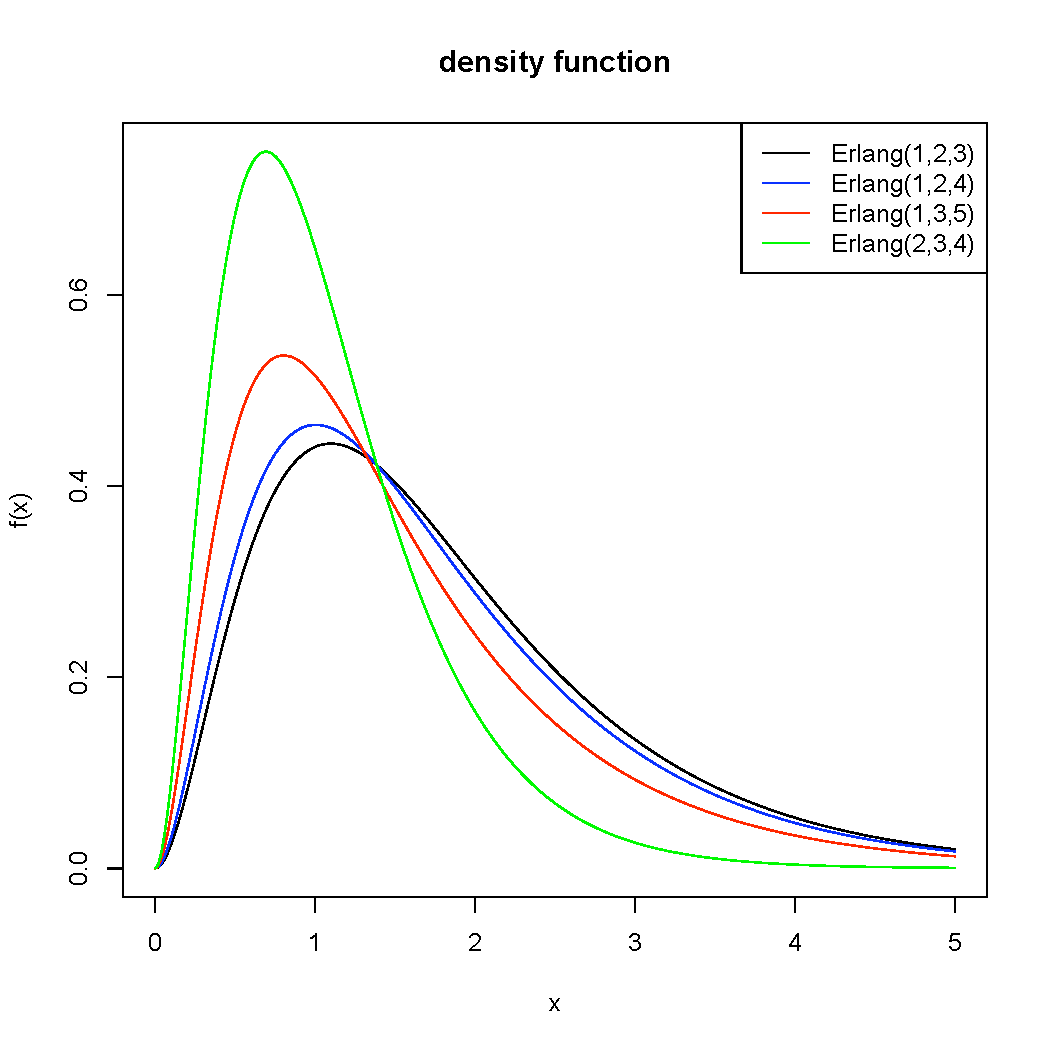
\includegraphics[width=0.48\textwidth]{img/generlangzoom}
  \end{center}
  \vspace{-20pt}  
  \caption{Density function for generalized Erlang distributions}
    \vspace{-20pt}  
\end{wrapfigure}

As the gamma distribution is the distribution of the sum of i.i.d. exponential distributions, the generalized Erlang distribution is the distribution of the sum independent exponential distributions. Sometimes it is called the hypoexponential distribution. The density is defined as 
$$
f(x) = \sum\limits_{i=1}^{d} \left( \prod\limits_{j=1,j\neq i}^d \frac{\lambda_j }{\lambda_j -\lambda_i} \right)\lambda_i e^{-\lambda_i x},
$$
where $x\geq 0$ and $\lambda_j>0$'s\footnote{with the constraint that all $\lambda_j$'s are strictly different.} are the paremeters (for each exponential distribution building the generalized Erlang distribution). There is an explicit form for the distribution function:
$$
F(x) = \sum\limits_{i=1}^{d} \left( \prod\limits_{j=1,j\neq i}^d \frac{\lambda_j }{\lambda_j -\lambda_i} \right)(1-e^{-\lambda_i x}).
$$
This distribution is noted $\mcal Erlang(\lambda_1,\dots, \lambda_d)$. Of course, we retrieve the Erlang distribution when $\forall i, \lambda_i=\lambda$.

Finally, the characteristic and moment generating functions of generalized Erlang distribution are
$$
\phi(t) = \prod\limits_{j=1}^d \frac{\lambda_j  }{\lambda_j -i t} \txtm{and} M(t)=\prod\limits_{j=1}^d \frac{\lambda_j  }{\lambda_j -t}.
$$

\subsection{Properties}
The expectation of the generalized Erlang distribution is simply $E(X) =\sum\limits_{i=1}^d\frac{1}{\lambda_i}$ and its variance $Var(X) = \sum\limits_{i=1}^d\frac{1}{\lambda_i^2}$.
 
 
\subsection{Estimation}
NEED REFERENCE

\subsection{Random generation}
The algorithm is very easy simulate independently $d$ random variables exponentially $\mcal E(\lambda_j)$ distributed and sum them.

\subsection{Applications}
NEED REFERENCE

%%%%%%%%%%%%%%%%%%%%%%%%%%%%%%%%%%%%%%%%%%%%%%
\section{Chi-squared distribution}
A special case of the gamma distribution is the chi-squared distribution. See section \ref{chisquared}.


%%%%%%%%%%%%%%%%%%%%%%%%%%%%%%%%%%%%%%%%%%%%%%
\newpage
\section{Inverse Gamma}
\subsection{Characterization}
\begin{wrapfigure}{r}{0.5\textwidth}
  \vspace{-20pt}
  \begin{center}
    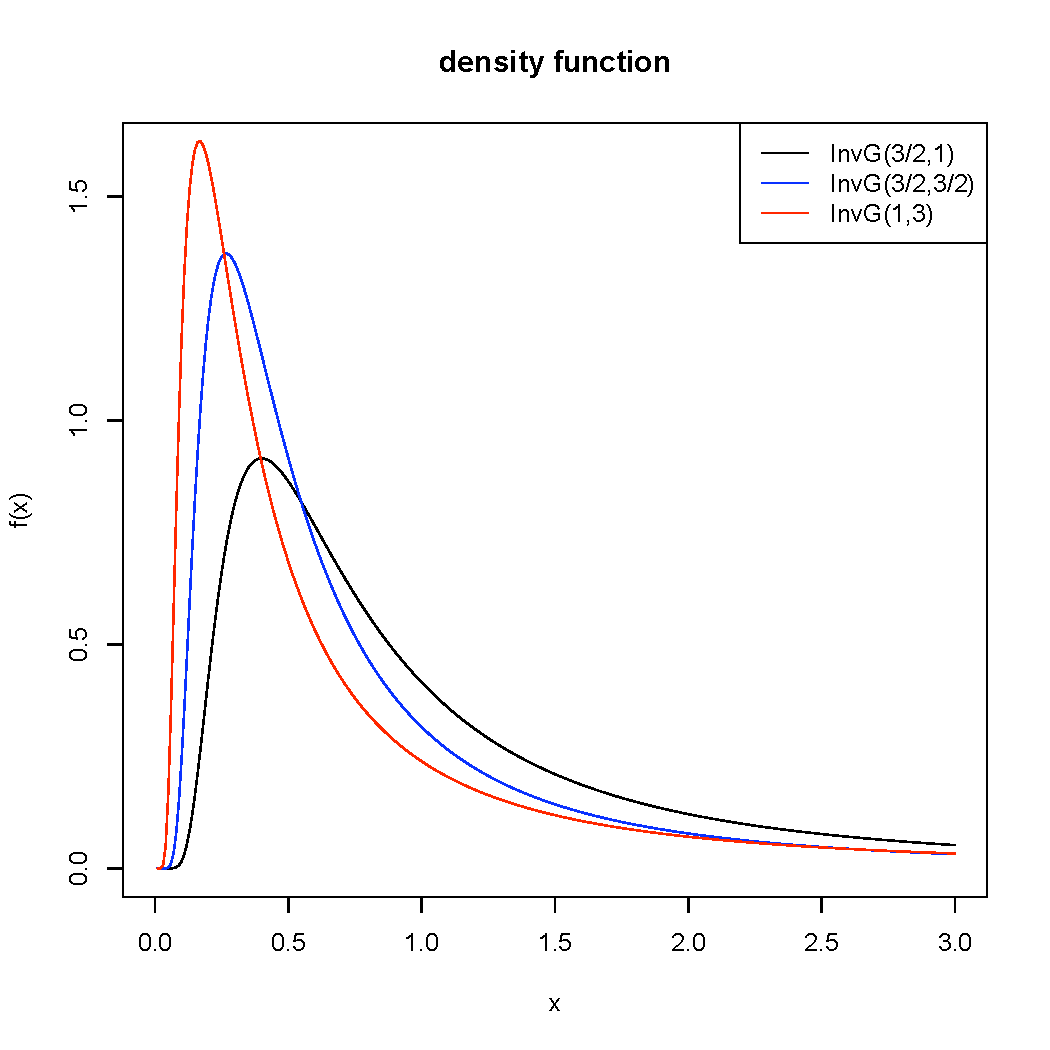
\includegraphics[width=0.48\textwidth]{img/invgammazoom}
  \end{center}
  \vspace{-20pt}  
  \caption{Density function for inverse gamma distributions}  
\end{wrapfigure}

The inverse gamma distribution is the distribution of a random variable $\frac{1}{X}$ when $X$ is gamma distributed. Hence the density is 
$$
f(x)=\frac{\lambda^\alpha}{\Gamma(\alpha)x^{\alpha+1}}e^{-\frac{\lambda}{x}},
$$
where $x>0$ and $\beta,\alpha>0$. From this, we can derive the distribution function 
$$
F(x)=\frac{\gamma(\alpha,\frac{\lambda}{x})}{\Gamma(\alpha)}.
$$

We can define inverse gamma distributions with characteristic or moment generating functions
$$
\phi(t)=\frac{2\sqrt{-it \lambda}^{\alpha}}{\Gamma(\alpha)} K_\alpha(2\sqrt{-i \lambda t})
$$
and
$$
M(t)=\frac{2\sqrt{-it \lambda}^{\alpha}}{\Gamma(\alpha)} K_\alpha(2\sqrt{-\lambda t}).
$$
where $K_.(.)$ denotes the modified Bessel function.

\subsection{Properties}
The expectation exists only when $\alpha>1$ and in this case $E(X)=\frac{\lambda}{\alpha-1}$, whereas the variance is only finite if $\alpha >2$ and $Var(X) = \frac{\lambda ^2}{(\alpha-1)^2(\alpha-2)}$.

\subsection{Estimation}
Method of moments give the following estimators
$$
\tilde \alpha = 2+\frac{(\bar X_n)^2}{S_n^2}
\txtm{and}
\tilde \lambda = \bar X_n(\tilde \alpha -1)
$$
with $\bar X_n$ and $S_n^2$ the sample mean and variance. If the variance does not exist, then $\alpha$ will be 2, it means we must use the maximum likelihood estimator (which works also for $\alpha\leq 2$).

Maximum likelihood estimators of $\alpha,\lambda$ verify the system
$$
\left\{
\begin{array}{l}
\log \alpha- \psi(\alpha)=    \log(\frac{1}{n}\sum_{i=1}^n \frac{1}{X_i}) -\frac{1}{n}\sum_{i=1}^n \log \frac{1}{X_i} \\
\lambda =\alpha \left(\frac{1}{n}\sum_{i=1}^n \frac{1}{X_i}\right)^{-1}
\end{array}
\right. ,
$$
where $\psi(.)$ denotes the digamma function. The first equation can be solved numerically\footnote{algorithm can be initialized with $\tilde \alpha$.} to get $\hat \alpha$ and then $\hat \lambda$ with the second equation.



\subsection{Random generation}
Simply generate a gamma variable $\mcal G(\alpha, 1/\lambda)$ and inverse it.

\subsection{Applications}
NEED REFERENCE



%%%%%%%%%%%%%%%%%%%%%%%%%%%%%%%%%%%%%%%%%%%%%%%%
\section{Transformed or generalized gamma}
\subsection{Characterization}
\begin{wrapfigure}{r}{0.5\textwidth}
  \vspace{-20pt}
  \begin{center}
    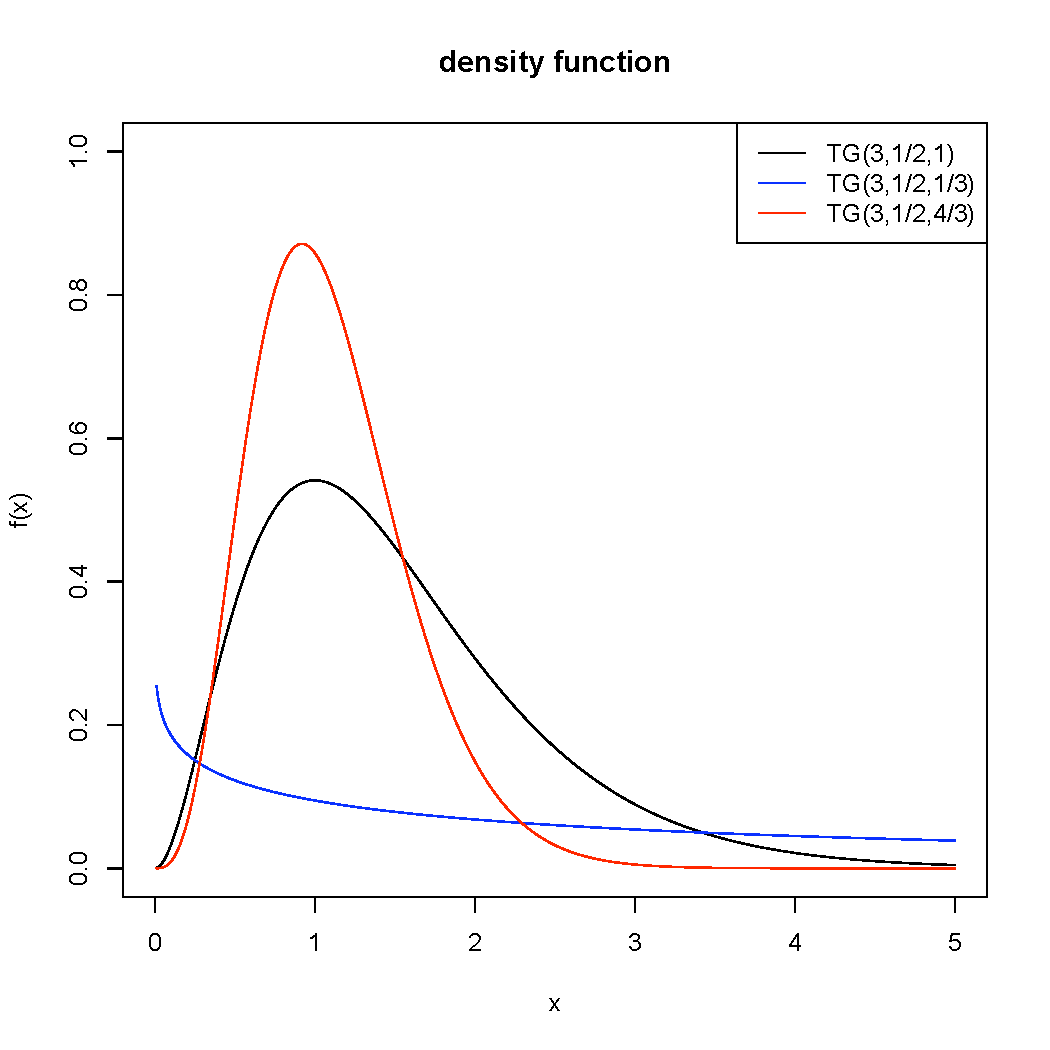
\includegraphics[width=0.48\textwidth]{img/transgammazoom}
  \end{center}
  \vspace{-20pt}  
  \caption{Density function for transformed gamma distributions}  
\end{wrapfigure}

The transformed gamma distribution is defined by the following density function
$$
f(x)=\frac{\tau (\frac{x}{\lambda})^{\alpha\tau-1} e^{-(\frac{x}{\lambda})^{\tau}} }{\lambda\Gamma(\alpha)},
$$
where $x>0$ and $\alpha, \lambda, \tau >0$. Thus, the distribution function is 
$$
F(x) = \frac{\gamma(\alpha,(\frac{x}{\lambda})^{\tau})}{\Gamma(\alpha)}.
$$
This is the distribution of the variable $\lambda X^{\frac{1}{\tau}}$ when $X$ is gamma distributed $\mcal G(\alpha,1)$.

Obviously, a special case of the transformed gamma is the gamma distribution with $\tau=1$. But we get the Weibull distribution with $\alpha=1$.

\subsection{Properties}
The expectation of the transformed gamma distribution is $E(X)=\frac{\lambda\Gamma(\alpha+\frac{1}{\tau})}{\Gamma(\alpha)}$ and its variance $Var(X)=\frac{\lambda^2\Gamma(\alpha+\frac{2}{\tau})}{\Gamma(\alpha)}-E^2[X]$.

From \cite{venter} moments are given by
$$
E(X^r) = \lambda^r \frac{\Gamma(\alpha+\frac{r}{\tau})}{\Gamma(\alpha)},
$$
with $\alpha+\frac{r}{\tau}>0$.

\subsection{Estimation}
Maximum likelihood estimators verify the following system
$$
\left\{
\begin{array}{l}
\psi(\alpha) - \log \alpha = \tau \frac{1}{n} \sum\limits_{i=1}^n \log X_i- \log(\frac{1}{n} \sum\limits_{i=1}^n X_i^\tau ) \\
\alpha = \frac{1}{n} \sum\limits_{i=1}^n X_i^\tau \left(  \frac{1}{n} \sum\limits_{i=1}^n X_i^\tau \log X_i -\left(\frac{1}{n} \sum\limits_{i=1}^n X_i^\tau \right) \left( \frac{1}{n} \sum\limits_{i=1}^n \log X_i\right) \right)^{-1} \\
\lambda = \left(\frac{1}{n} \sum\limits_{i=1}^n X_i^\tau \right)^\tau \alpha^{-\tau}
\end{array}
\right. ,
$$
where $\psi$ denotes the digamma function. This system can be solved numerically. 

TODO : use \cite{dussauchoy}

\subsection{Random generation}
Generate a gamma distributed variable ($\mcal G(\alpha,1)$),  raise it to power $\frac{1}{\tau}$ and multiply it by $\lambda$.

\subsection{Applications}
In an actuarial context, the transformed gamma may be useful in loss severity, for example, in workers' compensation, see \cite{venter}.

%%%%%%%%%%%%%%%%%%%%%%%%%%%%%%%%%%%%%%%%%%
\newpage
\section{Inverse transformed Gamma}
\subsection{Characterization}
\begin{wrapfigure}{r}{0.5\textwidth}
  \vspace{-20pt}
  \begin{center}
    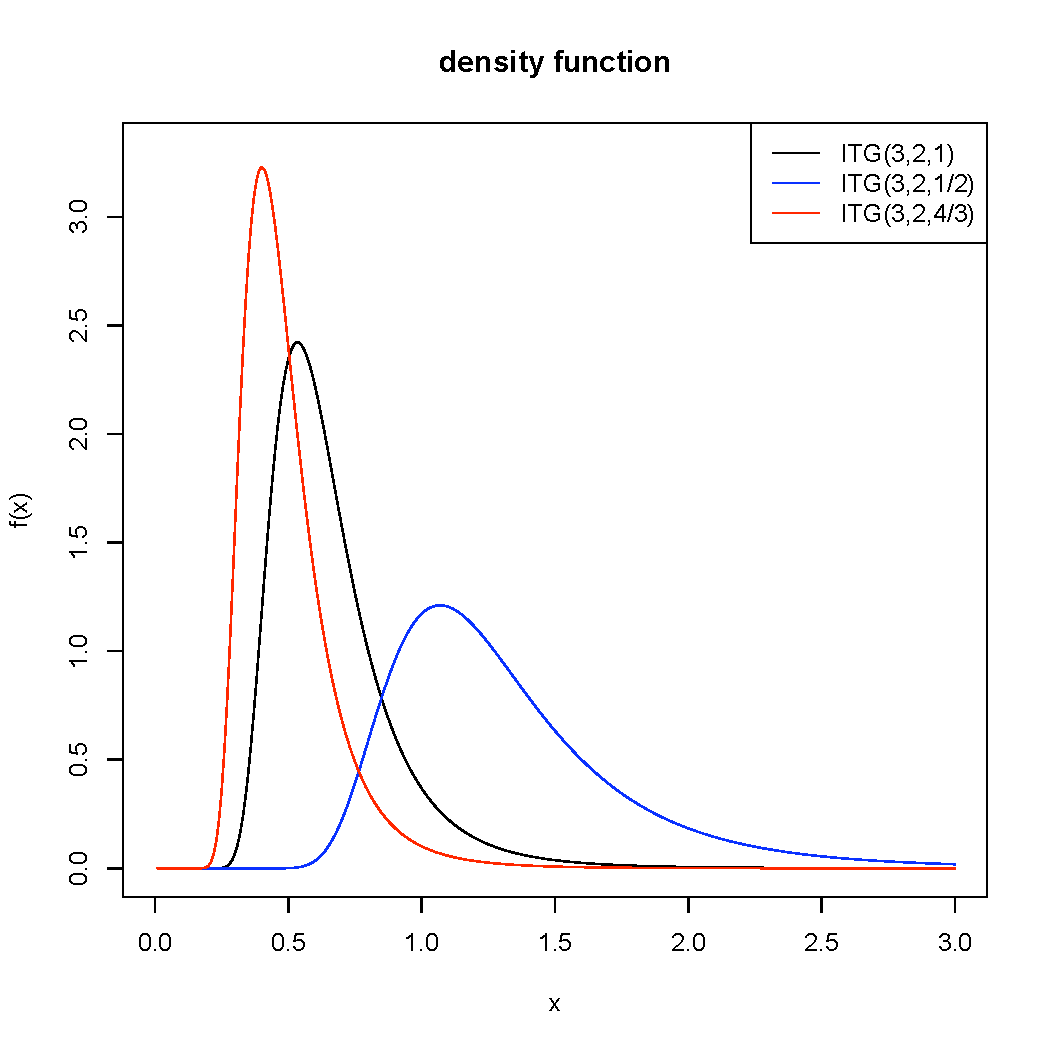
\includegraphics[width=0.48\textwidth]{img/invtrgammazoom}
  \end{center}
  \vspace{-20pt}  
  \caption{Density function for inverse transformed gamma distributions}  
\end{wrapfigure}
The transformed gamma distribution is defined by the following density function
$$
f(x)=\frac{\tau (\frac{\lambda}{x})^{\alpha\tau} e^{-(\frac{\lambda}{x})^{\tau}} }{x\Gamma(\alpha)},
$$
where $x>0$ and $\alpha, \lambda, \tau >0$. Thus, the distribution function is 
$$
F(x) = 1-\frac{\gamma(\alpha,(\frac{\lambda}{x})^{\tau})}{\Gamma(\alpha)}.
$$
This is the distribution of $\left(\frac{\lambda}{X}\right)^\frac{1}{\tau}$ when $X$ is gamma distributed $\mcal G(\alpha,1)$.
\subsection{Properties}
The expectation of the transformed gamma distribution is $E(X)=\frac{\lambda\Gamma(\alpha-\frac{1}{\tau})}{\Gamma(\alpha)}$ and its variance $Var(X)=\frac{\lambda^2\Gamma(\alpha-\frac{2}{\tau})}{\Gamma(\alpha)}-E^2[X]$.

From \cite{klugman}, we have the following formula for the moments
$$
E(X^r) = \frac{\lambda^r\Gamma(\alpha-\frac{r}{\tau})}{\Gamma(\alpha)}.
$$


\subsection{Estimation}
NEED REFERENCE
\subsection{Random generation}
Simply simulate a gamma $\mcal G(\alpha,1)$ distributed variable, inverse it, raise it to power $\frac{1}{\alpha}$ and multiply it by $\lambda$.

\subsection{Applications}
NEED REFERENCE

%%%%%%%%%%%%%%%%%%%%%%%%%%%%%%%%%%%%%%%%%%
\section{Log Gamma}
\subsection{Characterization}
Density function for log-gamma distribution is expressed as
$$
f(x) = \frac{e^{k\frac{x-a}{b} -e^{\frac{x-a}{b}} }}{\Gamma(k)}
$$
for $x>0$, where $a$ is the location parameter, $b>0$ the scale parameter and $k>0$ the shape parameter. The distribution function is 
$$
F(x) = \frac{\gamma(k, e^{\frac{x-a}{b}})}{\Gamma(k)},
$$
for $x>0$. This is the distribution of $a+b\log(X)$ when $X$ is gamma $\mcal G(k,1)$.

\subsection{Properties}
The expectation is $E(X)=a+b\psi(k)$ and the variance $Var(X) =b^2\psi_1(k)$ where $\psi$ is the digamma function and $\psi_1$ the trigamma function.

\subsection{Estimation}
NEED REFERENCE

\subsection{Random generation}
Simply simulate a gamma $\mcal G(k,1)$ distributed variable and returns $a+b\log(X)$.

\subsection{Applications}
NEED REFERENCE


%%%%%%%%%%%%%%%%%%%%%%%%%%%%%%%%%%%%%%%%%%%
\section{Weibull distribution}\label{weibull}
\subsection{Characterization}
\begin{wrapfigure}{r}{0.5\textwidth}
  \vspace{-40pt}
  \begin{center}
    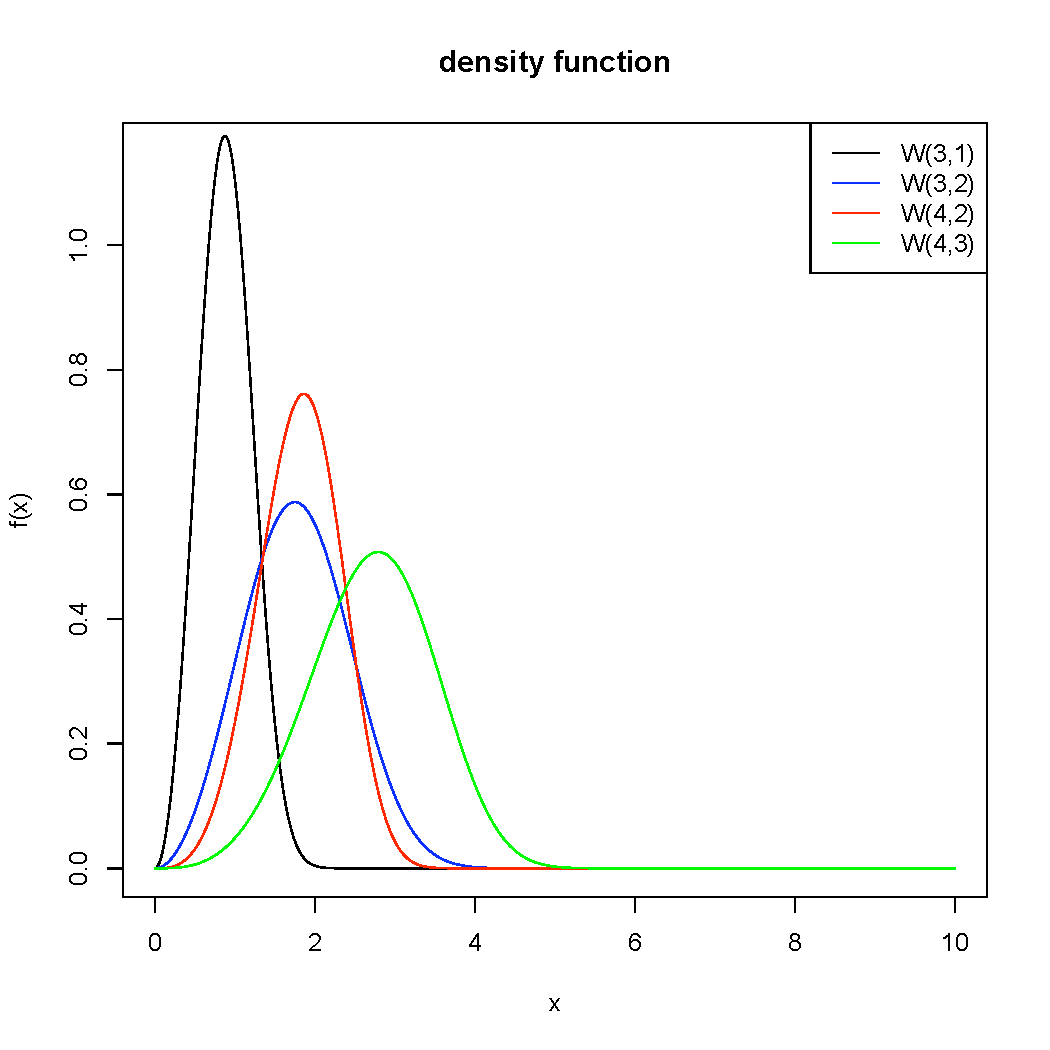
\includegraphics[width=0.48\textwidth]{img/weibullzoom}
  \end{center}
  \vspace{-20pt}  
  \caption{Density function for Weibull distributions}  
\end{wrapfigure}

Despite the fact the Weibull distribution is not particularly related to the chi distribution, its density tends exponentially fast to zero, as chi's related distribution. The density of a Weibull distribution is given by
$$
f(x) = \frac{\beta  }{\eta^{\beta}} x^{\beta-1} e^{-(\frac{x}{\eta})^{\beta}},
$$
where $x>0$ and $\eta, \beta >0$.
In terms of distribution function, the Weibull can be defined as
$$
F(x) =1-e^{-(\frac{x}{\beta})^\eta}.
$$

There exists a second parametrization of the Weibull distribution. We have
$$
f(x) = \tau \lambda x^{\lambda-1} e^{-\tau x^{\lambda}},
$$
with the same constraint on the parameters $\tau, \lambda >0$. In this context, the distribution function is 
$$
F(x) = 1-e^{-\tau x^{\lambda}}.
$$
We can pass from the first parametrization to the second one with
$$
\left\{
\begin{array}{c}
\lambda = \beta\\
\tau = \frac{1}{\eta^\beta}
\end{array}
\right. .
$$

\subsection{Properties}
The expectation of a Weibull distribution $\mathcal{ W}(\eta,\beta)$ is $E(X) = \eta \Gamma(1+\frac{1}{\beta})$ and the variance $Var(X) = \eta^2[\Gamma(\frac{\beta+2}{\beta})-\Gamma(\frac{\beta+1}{\beta})^2]$. In the second parametrization, we have $E(X) =  \frac{\tau(1+\frac{1}{\tau})}{\lambda^{\frac{1}{\tau}}}$ and $Var(X) = \frac{1}{\lambda^{\frac{2}{\tau}}}(\tau(1+\frac{2}{\tau}) - \tau(1+\frac{1}{\tau})^2)$.

The $r$th raw moment $E(X^r)$ of the Weibull distribution $\mathcal{ W}(\eta,\beta)$ is given by $\eta \Gamma(1+\frac{r}{\beta})$ for $r>0$.

The Weibull distribution is the distribution of the variable $\frac{X^\beta}{\eta}$ where $X$ follows an exponential distribution $\mathcal E(1)$.

\subsection{Estimation}
We work in this sub-section with the first parametrization. From the cumulative distribution, we have
$$
\log(-\log|1-F(x)|) = \beta\log x-\beta \log \eta.
$$
Thus we can an estimation of $\beta$ and $\eta$ by regressing $ \log(-\log{|\frac{i}{n}|})$ on $\log X_{i:n}$.
Then we get the following estimators
$$
\tilde \beta = \hat a \txtm{and} \tilde \eta = e^{-\frac{\hat b}{\hat a}},
$$
where $\hat a$ and $\hat b$ are respectively the slope and the intercept of the regression line.

The maximum likelihood estimators verify the following system
$$
\left\{
\begin{array}{l}
- \frac{n\beta}{\eta}+\frac{\beta}{\eta^{\beta+1}} \sum_{i=1}^{n}(x_i)^{\beta} = 0\\
 \frac{n}{\beta} -n\ln(\eta)+\sum_{i=1}^{n}\ln(x_i)-\sum_{i=1}^{n}\ln(x_i)(\frac{x_i}{\eta})^{\beta} = 0\\
\end{array}
\right. ,
$$
which can be solved numerically (with algorithm initialized by the previous estimators).

\subsection{Random generation}
Using the inversion function method, we simply need to compute $\beta(-\log(1-U))^{\frac{1}{\eta}}$ for the first parametrization or $\left(\frac{-\log(1-U)}{\tau}\right)^{\frac{1}{\lambda}}$ for the second one where $U$ is an uniform variate.

\subsection{Applications}
The Weibull was created by Weibull when he studied machine reliability.

NEED REFERENCE

%%%%%%%%%%%%%%%%%%%%%%%%%%%%%%%%%%%%%%%%%%%
\section{Inverse Weibull distribution}\label{invweibull}
\subsection{Characterization}
\begin{wrapfigure}{r}{0.5\textwidth}
  \vspace{-40pt}
  \begin{center}
    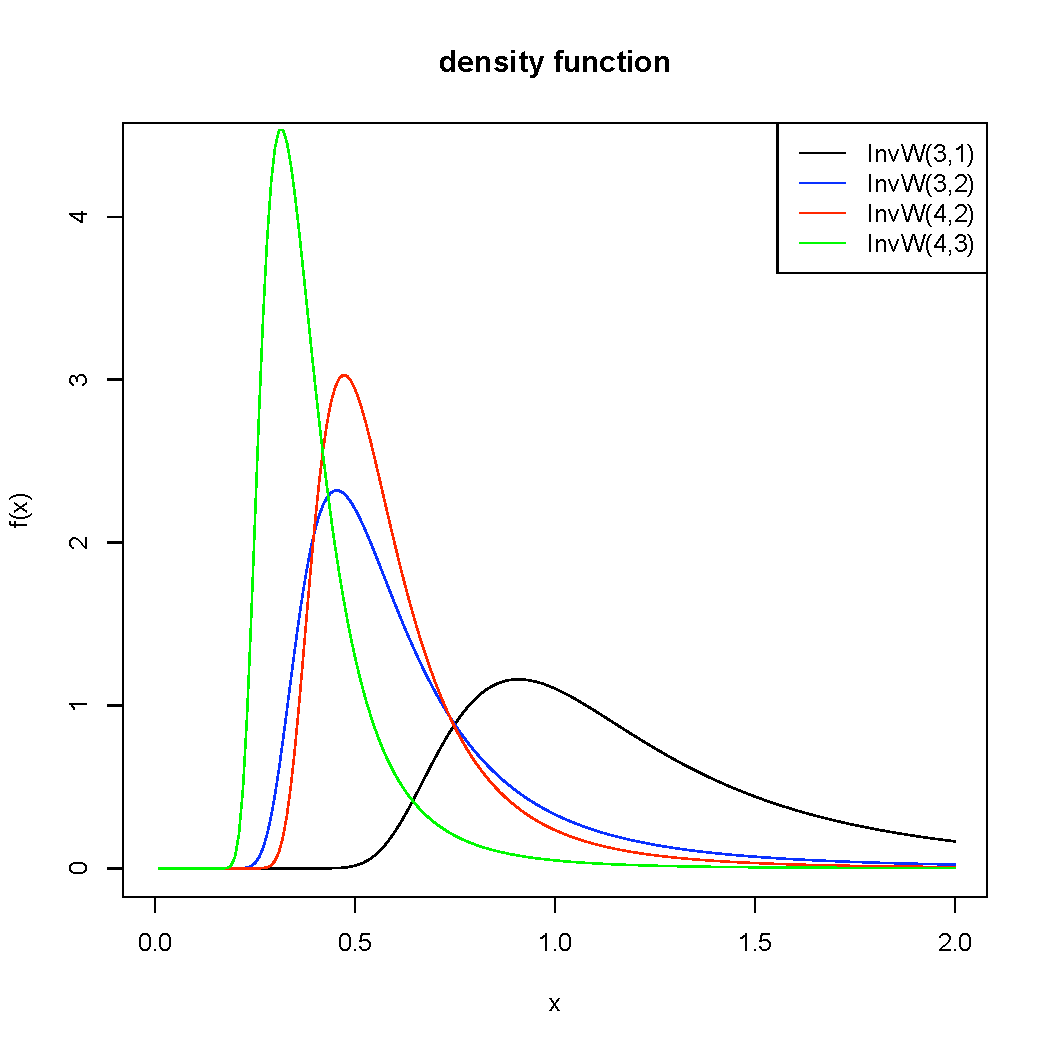
\includegraphics[width=0.48\textwidth]{img/invweibullzoom}
  \end{center}
  \vspace{-20pt}  
  \caption{Density function for inverse Weibull distributions}  
\end{wrapfigure}

The inverse Weibull distribution is defined as
$$
f(x) = \frac{\eta \beta^\eta e^{-(\frac{\beta}{x})^\eta} }{x^{\eta+1}},
$$
where $x>0$ and $\eta, \beta >0$. Its distribution function is
$$
F(x) = e^{-(\frac{\beta}{x})^\eta}.
$$
This is the distribution of $1/X$ when $X$ is Weibull distributed $\mcal W(\beta^{-1},\eta)$.

\subsection{Properties}
The expectation is given by $\eta \Gamma(1-\frac{1}{\beta})$ and the variance $\eta^2[\Gamma(\frac{\beta-2}{\beta})-\Gamma(\frac{\beta-1}{\beta})^2]$.

The $r$th moment of the Weibull distribution $\mathcal I\mathcal{W}(\eta,\beta)$ is given by $\eta^r \Gamma(1-\frac{r}{\beta})$ for $r>0$.

\subsection{Estimation}
Maximum likelihood estimators for $\beta$ and $\eta$ verify the following system
$$
\left\{
\begin{array}{l}
\frac{1}{\beta} = \frac{1}{n} \sum_{i=1}^n�\left( \frac{\beta}{X_i} \right)^{\eta-1} \\
\frac{1}{\eta} + \log(\beta) = \frac{1}{n} \sum_{i=1}^n \left( \frac{\beta}{X_i} \right)^{\eta} \log\left( \frac{\beta}{X_i} \right) + \frac{1}{n}\sum_{i=1}^n \log(X_i)
\end{array}
\right. ,
$$
while the method of moment has the following system
$$
\left\{
\begin{array}{l}
(S_n^2+(\bar X_n)^2) \Gamma^2(1-\frac{1}{\beta}) = (\bar X_n)^2 \Gamma(1-\frac{2}{\beta}) \\
\eta = \frac{\bar X_n}{\Gamma(1-\frac{1}{\beta})}
\end{array}
\right. .
$$
Both are to solve numerically.

\subsection{Random generation}
Simply generate a Weibull variable $\mcal W(\beta^{-1},\eta)$ and inverse it.

\subsection{Applications}
NEED REFERENCE

TODO \cite{ortega}

%%%%%%%%%%%%%%%%%%%%%%%%%%%%%%%%%%%%%%%%%%
\section{Laplace or double exponential distribution}
\subsection{Characterization}
\begin{wrapfigure}{r}{0.5\textwidth}
  \vspace{-20pt}
  \begin{center}
    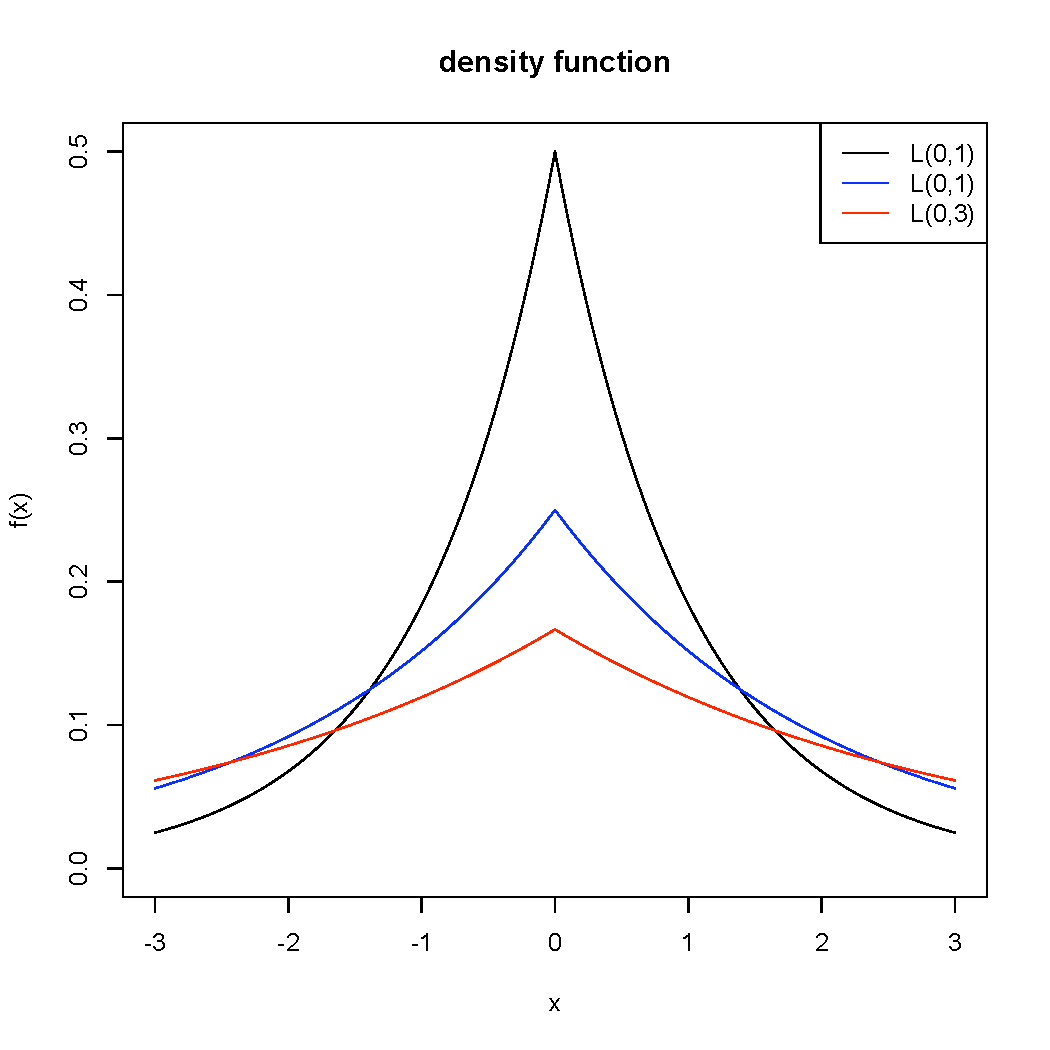
\includegraphics[width=0.48\textwidth]{img/laplacezoom}
  \end{center}
  \vspace{-20pt}  
  \caption{Density function for laplace distributions}  
\end{wrapfigure}

Density for the Laplace distribution is given by
$$
f(x) = \frac{1}{2\sigma^2} e^{-\frac{|x-m|}{\sigma} }, 
$$
for $x\in\mbb R$, $m$ the location parameter and $\sigma>0$ the scale parameter.
We have the following distribution function 
$$
F(x) = \left\{
\begin{array}{ll}
\frac{1}{2}e^{-\frac{m-x}{\sigma}} &\txtm{if} x<m\\
1-\frac{1}{2}e^{-\frac{x-m}{\sigma}} & \txtm{otherwise}\\
\end{array}
\right. .
$$
There exists a moment generating function for this distribution, which is
$$
M(t) = \frac{e^{mt}}{1-\sigma^2t^2},
$$
for $|t|< \frac{1}{\sigma}$.
The characteristic function is expressed as 
$$
\phi(t) = \frac{e^{imt}}{1+\sigma^2t^2},
$$
for $t\in\mbb R$.


\subsection{Properties}
The expectation for the Laplace distribution is given by $E(X) = m$ while the variance is $Var(X)=2\sigma^2$.

\subsection{Estimation}
Maximum likelihood estimators for $m$ and  $\sigma$ are 
$$
\hat m =\left\{
\begin{array}{ll}
\frac{X_{\frac{n}{2}:n}+X_{\frac{n+2}{2}:n}}{2} &\txtm{if} n \txtm{is even}\\
X_{\lfloor \frac{n}{2}\rfloor :n} & \txtm{otherwise}\\
\end{array}
\right. ,
$$
where $X_{k:n}$ denotes the $k$th order statistics and 
$$
\hat \sigma = \frac{1}{n} \sum_{i=1}^n|X_i -\hat m|.
$$

\subsection{Random generation}
Let $U$ be a uniform variate. Then the algorithm is
\begin{itemize}
\item $V = U-1/2$
\item $X=m+\sigma \textrm{sign}(V)\log(1-2|V|)$
\item return $X$
\end{itemize}


\subsection{Applications}
NEED 

 The Double Exponential Distribution: Using Calculus to Find a Maximum Likelihood Estimator
 Robert M. Norton
 The American Statistician, Vol. 38, No. 2 (May, 1984), pp. 135-136 


%----------------------------------------------------------------------------------------------------------
% 	Copyright (c) 2009 R-forge 'distributions' Core Team, 
% 	
%	The following Sweave code is under the GNU Free Documentation License:
%      	Permission is granted to copy, distribute and/or modify this document
%      	under the terms of the GNU Free Documentation License, Version 1.3
%      	or any later version published by the Free Software Foundation;
%      	with no Invariant Sections, no Front-Cover Texts, and no Back-Cover Texts.
%
%      A copy of the license is included in the 'inst' directory of this package 
%      or on the web at http://www.gnu.org/licenses/licenses.html#FDL
%
%	After running Sweave, the following code could be compiled :
%	  - on windows with a Tex distribution such as miktex (http://miktex.org) 
%		and a front end Latex editor such as texniccenter (http://www.toolscenter.org)
%	  - on mac os with a Tex distribution such as TexLive and a front end Latex
%	  	editor such as Texshop (http://www.uoregon.edu/~koch/texshop/)
%	  - on linux with a Tex distribution such as teTex (http://www.tug.org/teTeX/)
%	  	and a front end Latex editor such as emacs (http://www.gnu.org/software/emacs/)
%
%----------------------------------------------------------------------------------------------------------

\chapter{Chi-squared's ditribution and related extensions}
%%%%%%%%%%%%%%%%%%%%%%%%%%%%%%%%%%%%%%%%%%%%%%
\section{Chi-squared distribution}\label{chisquared}
\subsection{Characterization}
\begin{wrapfigure}{r}{0.5\textwidth}
  \vspace{-20pt}
  \begin{center}
    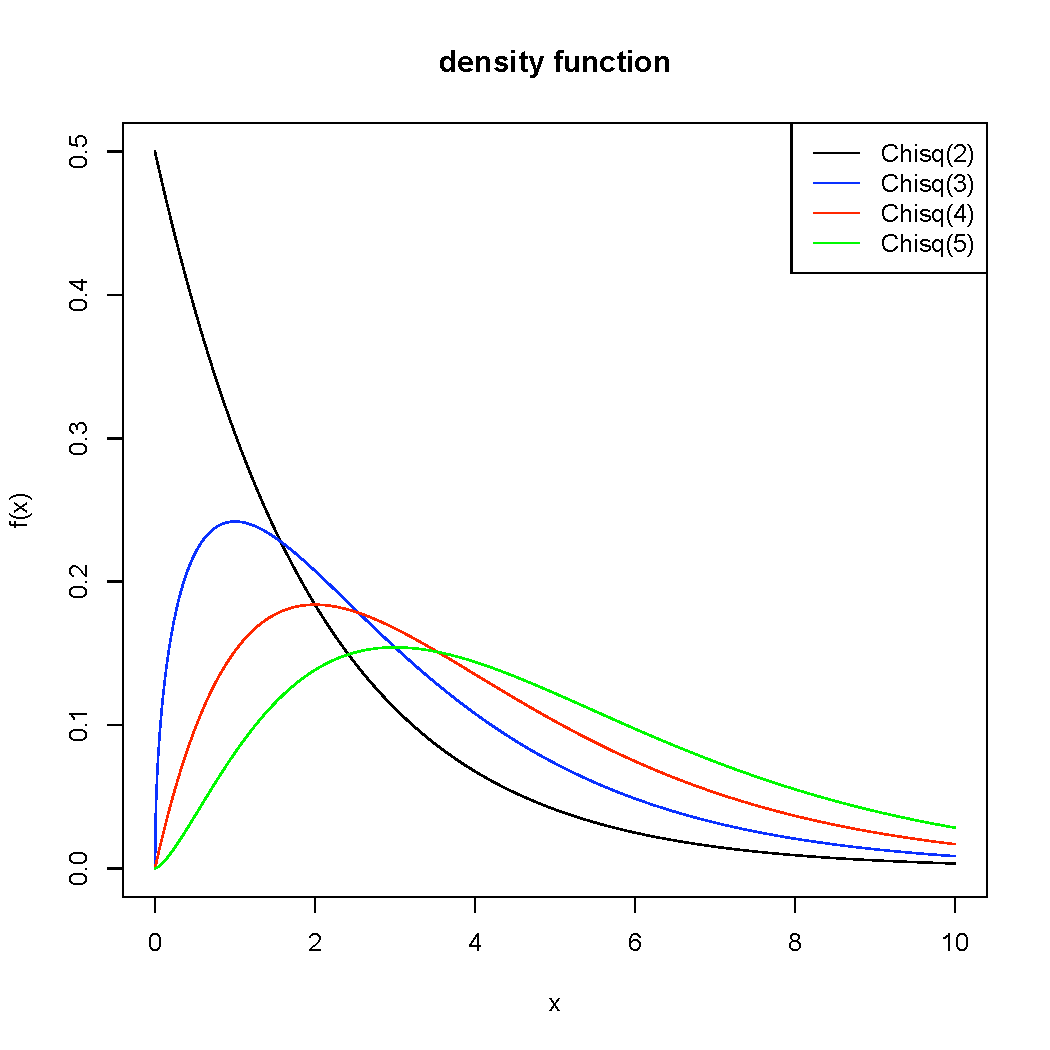
\includegraphics[width=0.48\textwidth]{img/chisqzoom}
  \end{center}
  \vspace{-20pt}  
  \caption{Density function for chi-squared distributions}
%  \vspace{-20pt}  
\end{wrapfigure}
There are many ways to define the chi-squared distribution. First, we can say a chi-squared distribution is the distribution of the sum
$$
\sum_{i=1}^k X_i^2,
$$
where $(X_i)_i$ are i.i.d. normally distributed $\mcal N(0,1)$ and a given $k$. In this context, $k$ is assumed to be an integer.

We can also define the chi-squared distribution by its density, which is
$$
f(x) = \frac{x^{\frac{k}{2}-1}}{\Gamma(\frac{k}{2}) 2^{\frac{k}{2}} }  e^{-\frac{x}{2} },  
$$
where $k$ is the so-called degrees of freedom and $x\geq 0$. One can notice that is the density of a gamma distribution $\mcal G(\frac{k}{2},\frac{1}{2})$, so $k$ is not necessarily an integer. Thus the distribution function can be expressed with the incomplete gamma function
$$
F(x) = \frac{\gamma(\frac{k}{2},\frac{x}{2})}{\Gamma(\frac{k}{2})}. 
$$

Thirdly, the chi-squared distribution can be defined in terms of its moment generating function
$$
M(t) = (1-2t)^{-\frac{k}{2}},
$$
or its characteristic function
$$
\phi(t) =(1-2it)^{-\frac{k}{2}}.
$$ 

\subsection{Properties}
The expectation and the variance of the chi-squared distribution are simply
$E(X) = k $ and $Var(X)=2k$. Raw moments are given by
$$
E(X^r) =\left(\frac{1}{2}\right)^r\frac{\Gamma(\frac{k}{2}+r)}{\Gamma(\frac{k}{2})}.
$$


\subsection{Estimation}
Same as gamma distribution ??

\subsection{Random generation}
For an integer $k$, just sum the square of $k$ normal variable. Otherwise use the algorithm for the gamma distribution.

\subsection{Applications}
The chi-squared distribution is widely used for inference, typically as pivotal function.

%%%%%%%%%%%%%%%%%%%%%%%%%%%%%%%%%%%%%%%%%%%%%%%%%
\newpage
\section{Chi distribution}
\subsection{Characterization}
\begin{wrapfigure}{r}{0.5\textwidth}
  \vspace{-20pt}
  \begin{center}
    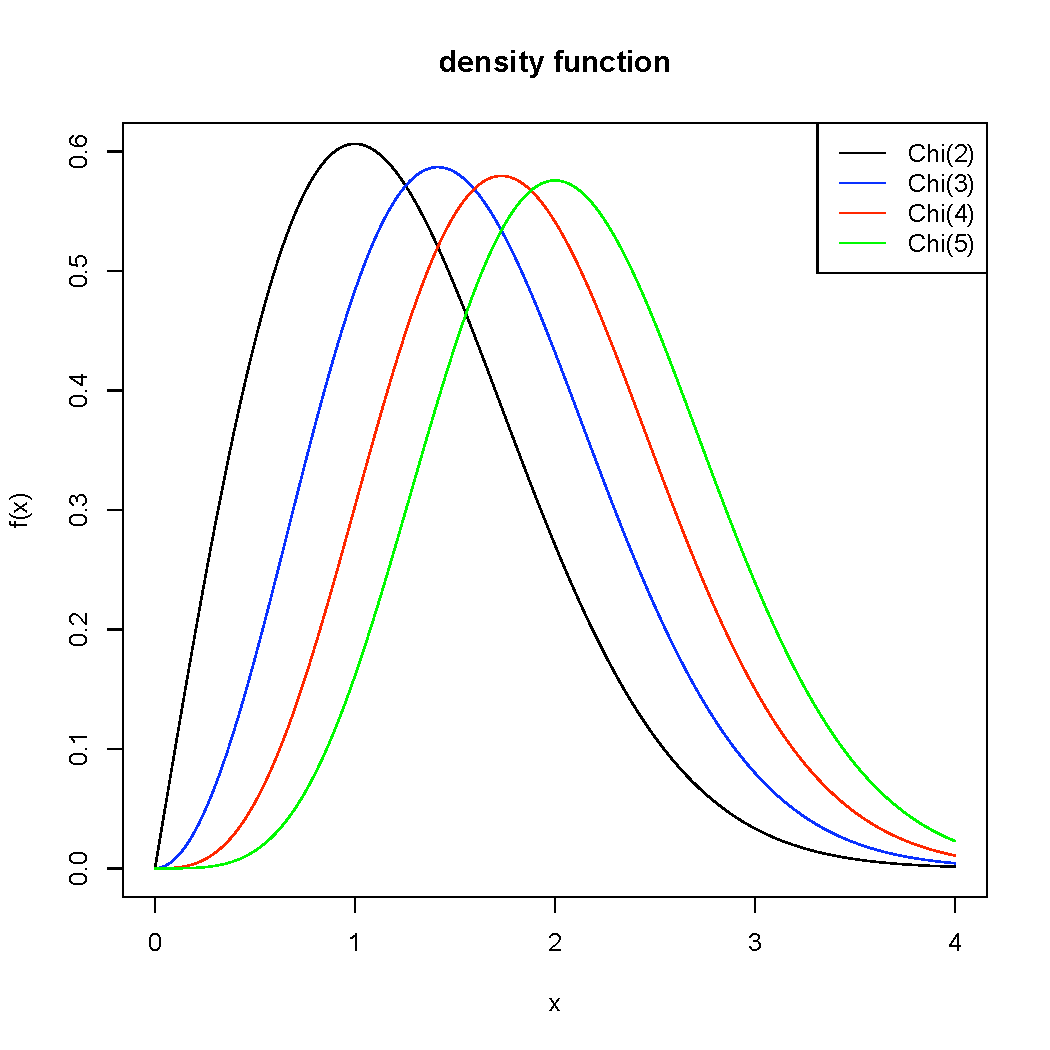
\includegraphics[width=0.48\textwidth]{img/chizoom}
  \end{center}
  \vspace{-20pt}  
  \caption{Density function for chi distributions}
%  \vspace{-20pt}  
\end{wrapfigure}
This is the distribution of the sum
$$
\sqrt{\sum_{i=1}^k X_i^2},
$$
where $(X_i)_i$ are i.i.d. normally distributed $\mcal N(0,1)$ and a given $k$. This is equivalent as the distribution of a square root of a chi-squared distribution (hence the name). 

The density function has a closed form
$$
f(x) = \frac{x^{k-1}}{2^{\frac{k}{2}-1}\Gamma\left(\frac{k}{2}\right)} e^{-\frac{x^2}{2}},
$$
where $x>0$.
The distribution function can be expressed in terms of the gamma incomplete function
$$
F(x) = \frac{\gamma(\frac{k}{2}, \frac{x^2}{2})}{\Gamma\left(\frac{k}{2}\right)},
$$
for $x>0$. 

Characteristic function and moment generating function exist and are expressed by
$$
\phi(t) = {\,}_1F_1\left(\frac{k}{2},\frac{1}{2},\frac{-t^2}{2}\right)+it\sqrt{2}\frac{\Gamma\left(\frac{k+1}{2}\right)}{\Gamma\left(\frac{k}{2}\right)} 
$$
and
$$
M(t) = {\,}_1F_1\left(\frac{k}{2},\frac{1}{2},\frac{t^2}{2}\right) +t\sqrt{2}\frac{\Gamma\left(\frac{k+1}{2}\right)}{\Gamma\left(\frac{k}{2}\right)}.
$$


\subsection{Properties}
The expectation and the variance of a chi distribution are given by $E(X) =\frac{\sqrt{2} \Gamma(\frac{k+1}{2})}{ \Gamma(\frac{k}{2})} $ and $Var(X) = k-E^2(X)$. Other moments are given by
$$
E(X^r) = 2^{\frac{r}{2}}\frac{ \Gamma(\frac{k+r}{2})}{ \Gamma(\frac{k}{2})},
$$
for $k+r>0$.

\subsection{Estimation}
The maximum likelihood estimator of $k$ satisfies the following equation
$$
\frac{1}{2}\psi\left(\frac{k}{2}\right)+ \frac{\log(2)}{2} = \frac{1}{n}\sum_{i=1}^n\log(X_i),
$$
where $\psi$ denotes the digamma function. This equation can be solved on the positive real line or just the set of positive integers.

\subsection{Random generation}
Take the square root of a chi-squared random variable.

\subsection{Applications}
NEED REFERENCE

%%%%%%%%%%%%%%%%%%%%%%%%%%%%%%%%%%%%%%%%%%%%%%%%%%%%
\section{Non central chi-squared distribution}

\subsection{Characterization}
\begin{wrapfigure}{r}{0.5\textwidth}
  \vspace{-20pt}
  \begin{center}
    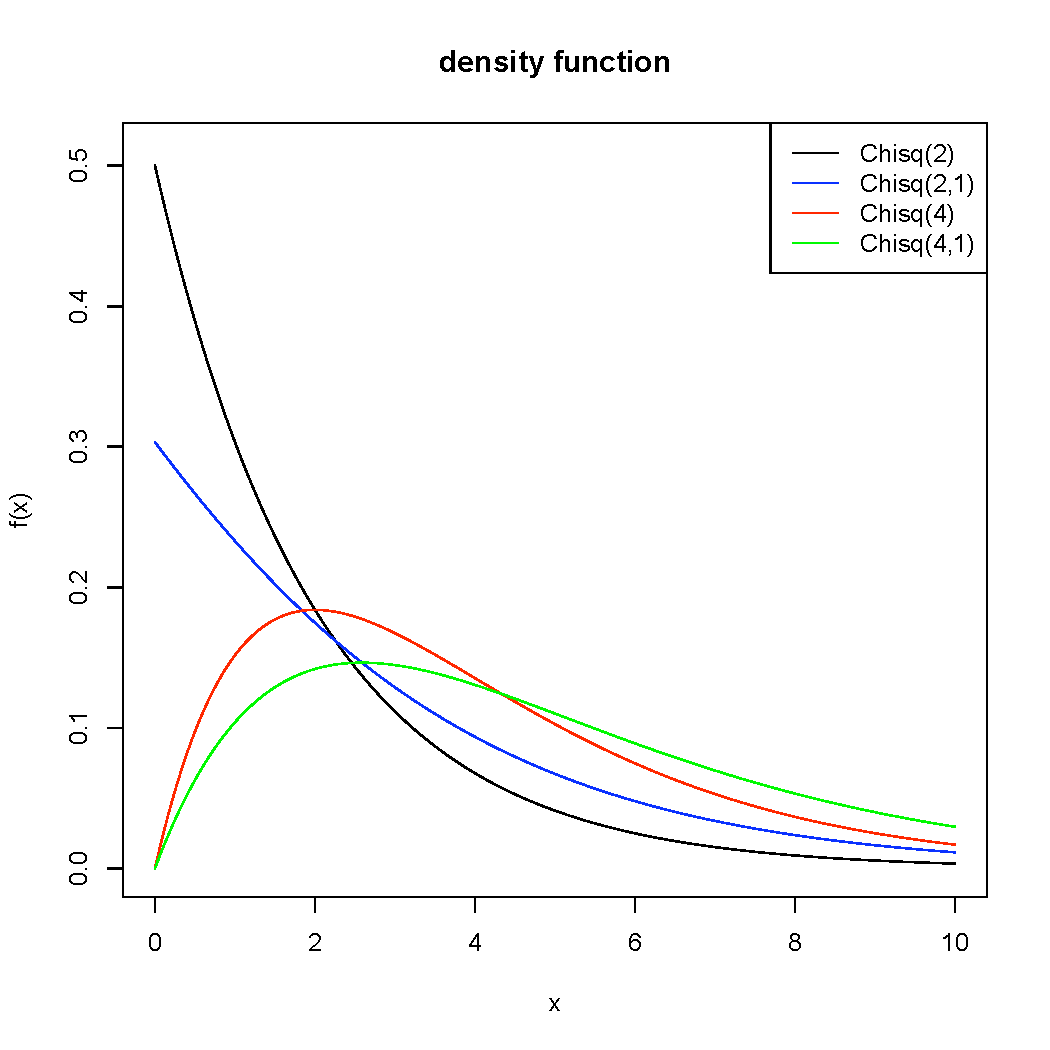
\includegraphics[width=0.48\textwidth]{img/noncentrchisqzoom}
  \end{center}
  \vspace{-20pt}  
  \caption{Density function for non central chi-squared distributions}
%  \vspace{-20pt}  
\end{wrapfigure}
The non central chi-squared distribution is the distribution of the sum
$$
\sum_{i=1}^k X_i^2,
$$
where $(X_i)_i$ are independent normally distributed $\mcal N(\mu_i,1)$, 
i.e. non centered normal random variable. We generally define the non central
chi-squared distribution by the density
$$
f(x) =  \frac{1}{2} \left(\frac{x}{\lambda}\right)^{\frac{k-2}{4}}  e^{-\frac{x+\lambda}{2} } I_{\frac{k}{2}-1} \left(\sqrt{\lambda x}\right) ,
$$
for $x>0$, $k\geq 2$ the degree of freedom, $\lambda$ the non central parameter and $I_\lambda$ the Bessel's modified function. $\lambda$ is related to the previous sum by 
$$
\lambda = \sum_{i=1}^k \mu_i^2.
$$

The distribution function can be expressed in terms of a serie
$$
F(x) = \sum_{j=0}^{+\infty} e^{\frac{-\lambda}{2}} \frac{(\frac{\lambda}{2})^j \gamma(j+\frac{k}{2},\frac{x}{2})}{j!\Gamma(j+\frac{k}{2})} ,
$$
for $x>0$ where $\gamma(.,.)$ denotes the incomplete gamma function.

Moment generating function for the non central chi-squared distribution exists
$$
M(t) = \frac{e^{\frac{\lambda  t}{1-2t}}}{(1-2t)^{\frac{k}{2}}}
$$
and the characteristic function
$$
\phi(t) = \frac{e^{\frac{\lambda i t}{1-2it}}}{(1-2it)^{\frac{k}{2}}},
$$
from which we see it is a convolution of a gamma distribution and a compound Poisson distribution.

\subsection{Properties}
Moments for the non central chi-squared distribution are given by
$$
E(X^n) = 2^{n-1}(n-1)!(k+n\lambda)+\sum_{j=1}^{n-1} \frac{(n-1)!2^{j-1}}{(n-j)!}(k+j\lambda )E(X^{n-j}),
$$
where the first raw moment is
$$
E(X) = k+\lambda. 
$$
The variance is $Var(X) = 2(k+2\lambda)$.


\subsection{Estimation}
\cite{liyu} and \cite{saxena}

\subsection{Random generation}
For integer $k$ degrees of freedom, we can use the definition of the sum, i.e. sum $k$ idependent normal random variables $\mcal N(\sqrt{\frac{\lambda}{k}},1)$.

\subsection{Applications}
NEED REFERENCE

%%%%%%%%%%%%%%%%%%%%%%%%%%%%%%%%%%%%%%%%%%
\section{Non central chi distribution}
\subsection{Characterization}

This is the distribution of the sum
$$
\sqrt{\sum_{i=1}^k X_i^2},
$$
where $(X_i)_i$ are i.i.d. normally distributed $\mcal N(\mu_i,1)$ and a given $k$. This is equivalent as the distribution of a square root of a non central chi-squared distribution (hence the name). 

We generally define the non central chi distribution by
$$
f(x) = \frac{\lambda x^{k}}{(\lambda x)^{\frac{k}{2}} } e^{-\frac{x^2+\lambda^2}{2}} I_{\frac{k}{2}-1}(\lambda x),
$$
where $x>0$ and $I_.(.)$ denotes the modified Bessel's function.
The distribution function can be expressed in terms of the gamma incomplete function
$$
F(x) = ??,
$$
for $x>0$. 




\subsection{Properties}
The expectation and the variance of a chi distribution are given by $$
E(X) =\sqrt{\frac{\pi}{2}}L_{1/2}^{(k/2-1)}\left(\frac{-\lambda^2}{2}\right)
$$ and $$
Var(X) = k+\lambda^2-E^2(X), $$
where $L_.^{(.)}$ denotes the generalized Laguerre polynomials.
Other moments are given by
$$
E(X^r) = ??,
$$
for $k+r>0$.

\subsection{Estimation}
NEED REFERENCE

\subsection{Random generation}
NEED REFERENCE

\subsection{Applications}
NEED REFERENCE

%%%%%%%%%%%%%%%%%%%%%%%%%%%%%%%%%%%%%%%%%%%%%%%
\section{Inverse chi-squared distribution}
\begin{wrapfigure}{r}{0.5\textwidth}
  \vspace{-20pt}
  \begin{center}
    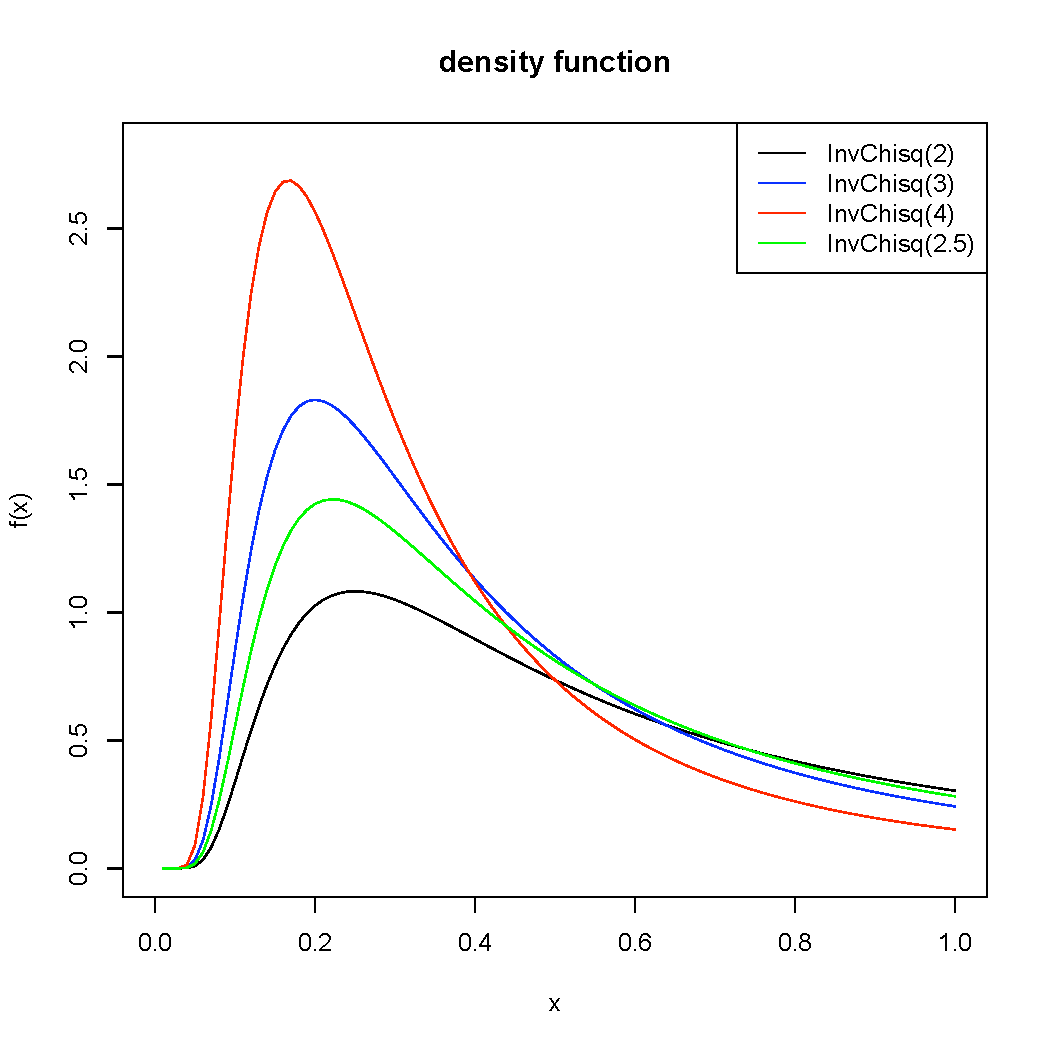
\includegraphics[width=0.48\textwidth]{img/invchisqzoom}
  \end{center}
  \vspace{-20pt}  
  \caption{Density function for inverse chi-squared distributions}
%  \vspace{-20pt}  
\end{wrapfigure}
The inverse chi-squared distribution is simply the distribution of $\frac{1}{X}$ when $X$ is chi-squared distributed.
We can also define the chi-squared distribution by its density, which is
$$
f(x) = \frac{2^{-\frac{k}{2}}}{\Gamma(\frac{k}{2})}\,x^{-\frac{k-2}{2}}  e^{-\frac{1}{2x}},
$$
where $k$ is the so-called degrees of freedom and $x\geq 0$. Thus the distribution function can be expressed with the incomplete gamma function
$$
F(x) = \frac{\Gamma(\frac{k}{2},\frac{1}{2x})}{\Gamma(\frac{k}{2})},
$$
where $\Gamma(.,.)$ the upper incomplete gamma function.

Thirdly, the chi-squared distribution can be defined in terms of its moment generating function
$$
M(t) = \frac{2}{\Gamma(\frac{k}{2})} \left(\frac{-t}{2}\right)^{\!\!\frac{k}{4}} K_{\frac{k}{2}}\!\left(\sqrt{-2t}\right),
$$
or its characteristic function
$$
\phi(t) =\frac{2}{\Gamma(\frac{k}{2})} \left(\frac{-it}{2}\right)^{\!\!\frac{k}{4}} K_{\frac{k}{2}}\!\left(\sqrt{-2it}\right).
$$ 

\subsection{Properties}
The expectation and the variance of the chi-squared distribution are simply
$E(X) = \frac{1}{k-2} $ if $k>2$ and $Var(X)=\frac{2}{(k-2)^2(k-4)}$. Raw moments are given by
$$
E(X^r) =??
$$


\subsection{Estimation}
Maximum likelihood estimator for $k$ verifies the equation
$$
\psi\left(\frac{k}{2}\right) = -\log(2)-\frac{1}{n}\sum_{i=1}^n \log(x_i),
$$
where $\psi$ denotes the digamma function.

\subsection{Random generation}
Simply inverse a chi-squared random variable

\subsection{Applications}
NEED REFERENCE

%%%%%%%%%%%%%%%%%%%%%%%%%%%%%%%%%%%%%%%%%%%%%
\section{Scaled inverse chi-squared distribution}
\subsection{Characterization}
TODO
\subsection{Properties}
TODO
\subsection{Estimation}
TODO
\subsection{Random generation}
TODO
\subsection{Applications}
TODO

%----------------------------------------------------------------------------------------------------------
% 	Copyright (c) 2009 R-forge 'distributions' Core Team, 
% 	
%	The following Sweave code is under the GNU Free Documentation License:
%      	Permission is granted to copy, distribute and/or modify this document
%      	under the terms of the GNU Free Documentation License, Version 1.3
%      	or any later version published by the Free Software Foundation;
%      	with no Invariant Sections, no Front-Cover Texts, and no Back-Cover Texts.
%
%      A copy of the license is included in the 'inst' directory of this package 
%      or on the web at http://www.gnu.org/licenses/licenses.html#FDL
%
%	After running Sweave, the following code could be compiled :
%	  - on windows with a Tex distribution such as miktex (http://miktex.org) 
%		and a front end Latex editor such as texniccenter (http://www.toolscenter.org)
%	  - on mac os with a Tex distribution such as TexLive and a front end Latex
%	  	editor such as Texshop (http://www.uoregon.edu/~koch/texshop/)
%	  - on linux with a Tex distribution such as teTex (http://www.tug.org/teTeX/)
%	  	and a front end Latex editor such as emacs (http://www.gnu.org/software/emacs/)
%
%----------------------------------------------------------------------------------------------------------

\chapter{Student and related distributions}
%%%%%%%%%%%%%%%%%%%%%%%%%%%%%%%%%%%%%%%%%%%%%
\section{Student t distribution}
Intro?
\subsection{Characterization}
\begin{wrapfigure}{r}{0.5\textwidth}
  \vspace{-20pt}
  \begin{center}
    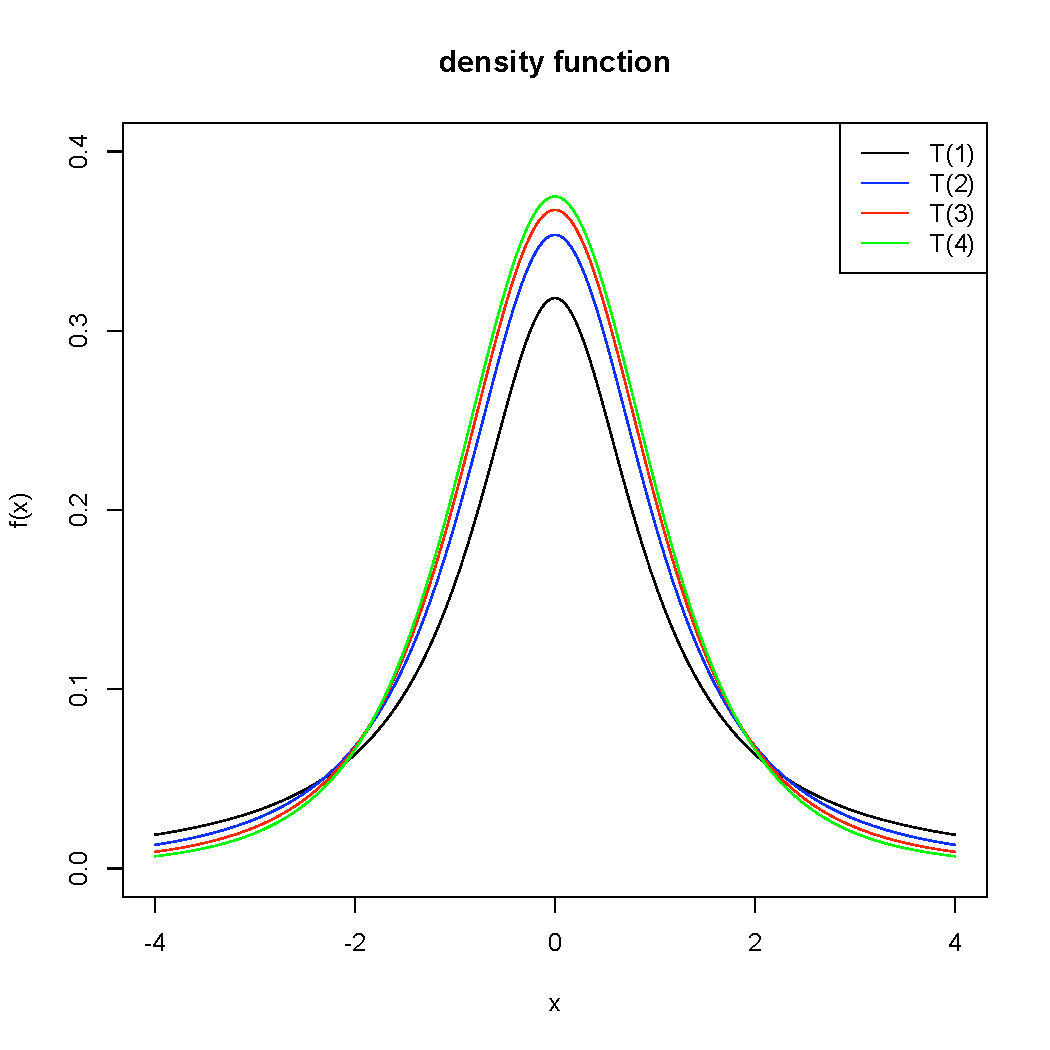
\includegraphics[width=0.48\textwidth]{img/studentzoom}
  \end{center}
  \vspace{-20pt}  
  \caption{Density function for student distributions}
%  \vspace{-20pt}  
\end{wrapfigure}

There are many ways to define the student distribution. One can say that it is the distribution of
$$
\frac{\sqrt{d}N}{C},
$$
where $N$ is a standard normal variable independent of $C$ a chi-squared variable with $d$ degrees of freedom. We can derive the following density function
$$
f(x) =  \frac{\Gamma(\frac{d+1}{2})}{\sqrt{\pi d} \Gamma(\frac{d}{2}) } \left(1+\frac{x^2}{d}\right)^{-\frac{d+1}{2}},
$$
for $x\in\mbb R$. $d$ is not necessarily an integer, it could be a real but greater than 1.

The distribution function of the student t distribution is given by
$$
F(x) = \frac{1}{2} + x \Gamma \left( \frac{d+1}{2} \right) \frac{ \,_2F_1 \left ( \frac{1}{2},\frac{d+1}{2};\frac{3}{2}; -\frac{x^2}{d} \right)}   {\sqrt{\pi\nu}\,\Gamma (\frac{d}{2})},
$$
where $\,_2F_1$ denotes the hypergeometric function.

\subsection{Properties}
The expectation of a student distribution is $E(X)=0$ if $d>1$, infinite otherwise. And the variance is given by $Var(X) = \frac{d}{d-2}$ if $d>2$.

Moments are given by
$$
E(X^r) = \prod_{i=1}^{r/2} \frac{2i-1}{\nu - 2i}\nu^{r/2},
$$
where $r$ is an even integer.

\subsection{Estimation}
Maximum likelihood estimator for $d$ can be found by solving numerically this equation
$$
\psi\left ( \frac{d+1}{2}\right) - \psi\left ( \frac{d}{2}\right) = \frac{1}{n}\sum_{i=1}^n\log\left(1+\frac{X_i^2}{d}\right) - \frac{d+1}{n} \sum_{i=1}^n \frac{(X_i/d)^2}{1+X_i^2/d},
$$
where $\psi$ denotes the digamma function.

\subsection{Random generation}
The algorithm is simply
\begin{itemize}
\item generate a standard normal distribution $N$
\item generate a chi-squared distribution $C$
\item return $\frac{\sqrt{d}N}{\sqrt{C}}$.
\end{itemize}

\subsection{Applications}
The main application of the student is when dealing with a normally distributed sample, the derivation of the  confidence interval for the standard deviation use the student distribution. Indeed for a normally distributed $\mcal N(m,\sigma^2)$ sample of size $n$ we have that  
$$
\frac{\bar X_n-m}{\sqrt{S_n^2}}\sqrt{n}
$$ 
follows a student $n$ distribution.

%%%%%%%%%%%%%%%%%%%%%%%%%%%%%%%%%%%%%%%%%%%%%
\section{Cauchy distribution}
\subsection{Characterization}
\subsection{Characterization}
\begin{wrapfigure}{r}{0.5\textwidth}
  \vspace{-20pt}
  \begin{center}
    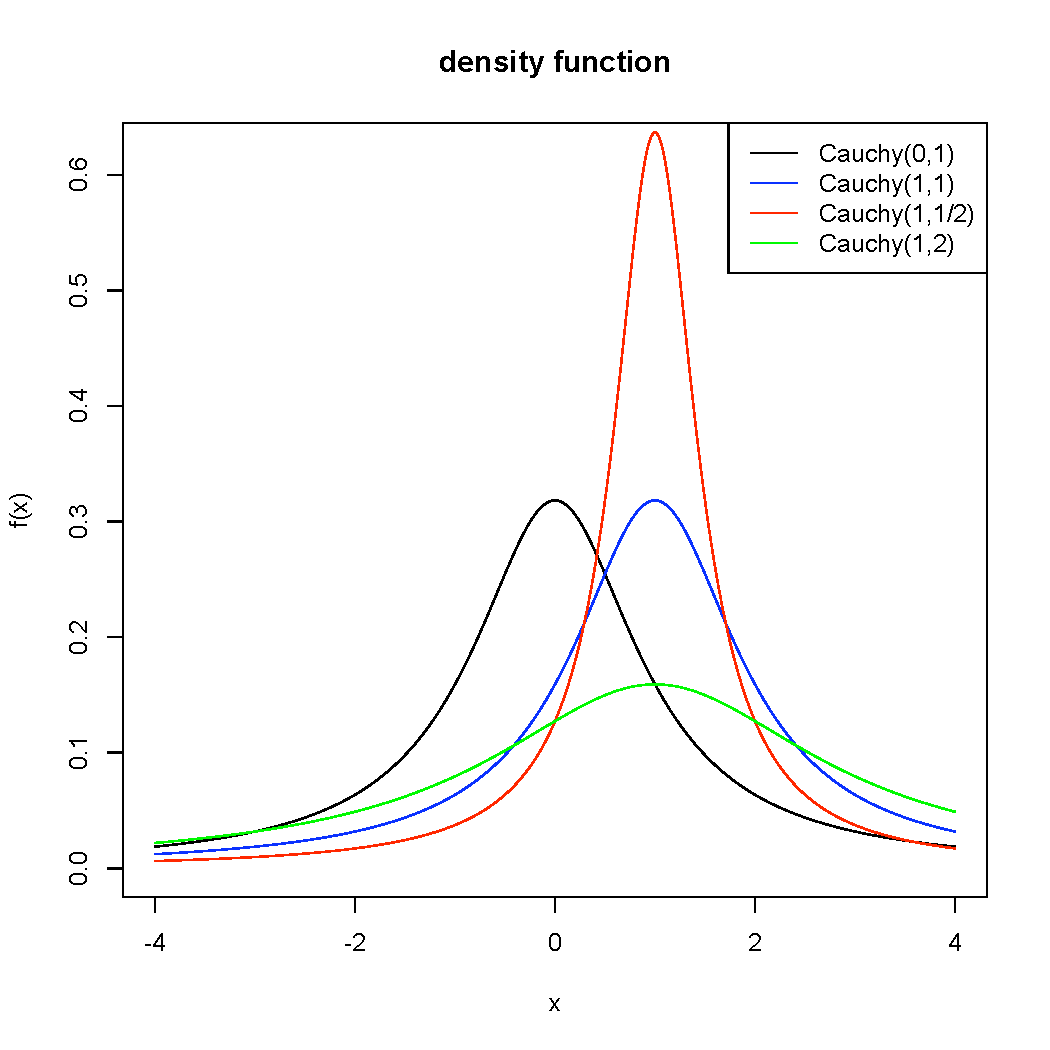
\includegraphics[width=0.48\textwidth]{img/cauchyzoom}
  \end{center}
  \vspace{-20pt}  
  \caption{Density function for Cauchy distributions}
%  \vspace{-20pt}  
\end{wrapfigure}
The Cauchy distribution is a special case of the Student distribution when a degree of freedom of $1$. Therefore the density function is
$$
f(x) =\frac{1}{\pi(1+x^2)},
$$
where $x\in \mathbb R$. Its distribution function is 
$$
F(x) = \frac{1}{\pi} \arctan(x)+\frac{1}{2}.
$$

There exists a scaled and shifted version of the Cauchy distribution coming from the scaled and shifted version of the student distribution. The density is
$$
f(x) = \frac{\gamma^2}{\pi \left[\gamma^2 + (x-\delta)^2\right]},
$$
while its distribution function is 
$$
F(x) = \frac{1}{\pi} \arctan\left(\frac{x-\delta}{\gamma}\right)+\frac{1}{2}.
$$
Even if there is no moment generating function, the Cauchy distribution has a characteristic function
$$
\phi(t) = \exp(\delta\,i\,t-\gamma\,|t|).
$$


\subsection{Properties}
The Cauchy distribution $\mathcal C(\delta, \gamma)$ has the horrible feature not to have any finite moments. However, the Cauchy distribution belongs to the family of stable distribution, thus a sum of Cauchy distribution is still a Cauchy distribution.

\subsection{Estimation}
Maximum likelihood estimators verify the following system
$$
\left\{
\begin{array}{l}
\frac{1}{\gamma} = \frac{1}{n} \sum\limits_{i=1}^n\frac{\gamma}{\gamma^2+(X_i-\delta)^2}\\
\sum\limits_{i=1}^n\frac{X_i}{\gamma^2+(X_i-\delta)^2} = \sum\limits_{i=1}^n\frac{\delta}{\gamma^2+(X_i-\delta)^2}\\
\end{array}
\right. .
$$
There is no moment based estimators.

\subsection{Random generation}
Since the quantile function is $F^{-1}(u) = \delta+\gamma\tan((u-1/2)\pi)$, we can use the inversion function method.

\subsection{Applications}
NEED REFERENCE


%%%%%%%%%%%%%%%%%%%%%%%%%%%%%%%%%%%%%%%%%%%%
\section{Fisher-Snedecor distribution}
\subsection{Characterization}
TODO
\subsection{Properties}
TODO
\subsection{Estimation}
TODO
\subsection{Random generation}
TODO
\subsection{Applications}
TODO
\chapter{Pareto family}
%%%%%%%%%%%%%%%%%%%%%%%%%%%%%%%%%%%%%%%%%%%%%
\section{Pareto distribution}
name??
\subsection{Characterization}
\begin{wrapfigure}{r}{0.5\textwidth}
  \vspace{-20pt}
  \begin{center}
    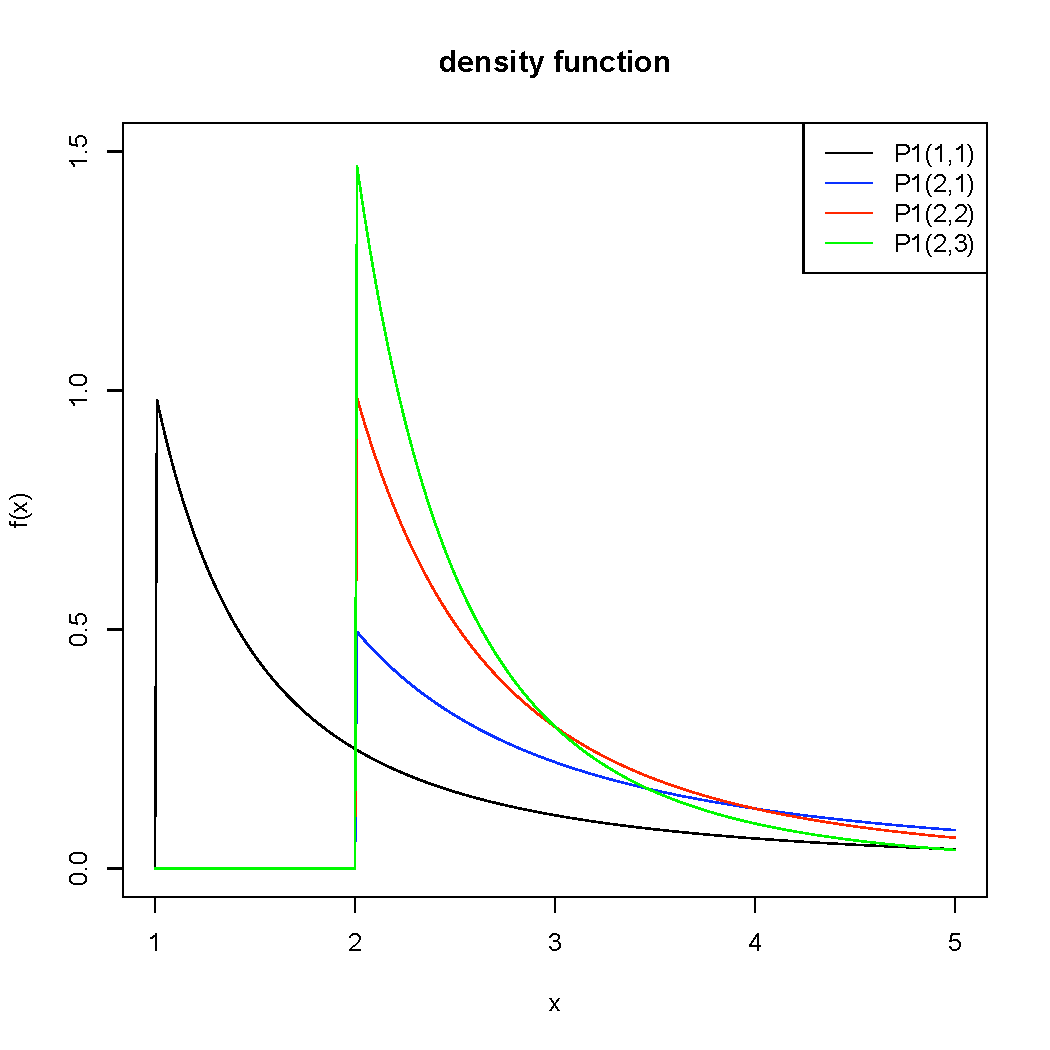
\includegraphics[width=0.48\textwidth]{img/pareto1zoom}
  \end{center}
  \vspace{-20pt}  
  \caption{Density function for Pareto I distributions}
  \vspace{-20pt}  
\end{wrapfigure}
The Pareto is widely used by statistician across the world, but many parametrizations of the Pareto distribution are used. Typically two different generalized Pareto distribution are used in extrem value theory with the work of Pickands et al. and in loss models by Klugman et al. To have a clear view on Pareto distributions, we use the work of \cite{arnold83}.
Most of the time, Pareto distributions are defined in terms of their survival function $\bar F$, thus we omit the distribution function. In the following, we will define Pareto type I, II, III and IV plus the Pareto-Feller distributions. 

\subsubsection{Pareto I}
The Pareto type I distribution $\mcal Pa_I(\sigma, \alpha)$ is defined by the following survival function
$$
\bar F(x) = \left(\frac{x}{\sigma}\right)^{-\alpha},
$$
where $x>\sigma$ and $\alpha>0$. Therefore, its density is 
$$
f(x) = \frac{\alpha}{\sigma} \left(\frac{x}{\sigma}\right)^{-\alpha-1},
$$
still for $x>\sigma$. $\alpha$ is the positive slope parameter\footnote{the slope of the Pareto chart $\log \bar F(x)$ vs. $\log x$, controlling the shape of the distribution.} (sometimes called the Pareto's index) and $\sigma$ is the scale parameter.
Pareto type I distribution is sometimes called the classical Pareto distribution or the European Pareto distribution.

\subsubsection{Pareto II}
\begin{wrapfigure}{r}{0.5\textwidth}
  \vspace{-40pt}
  \begin{center}
    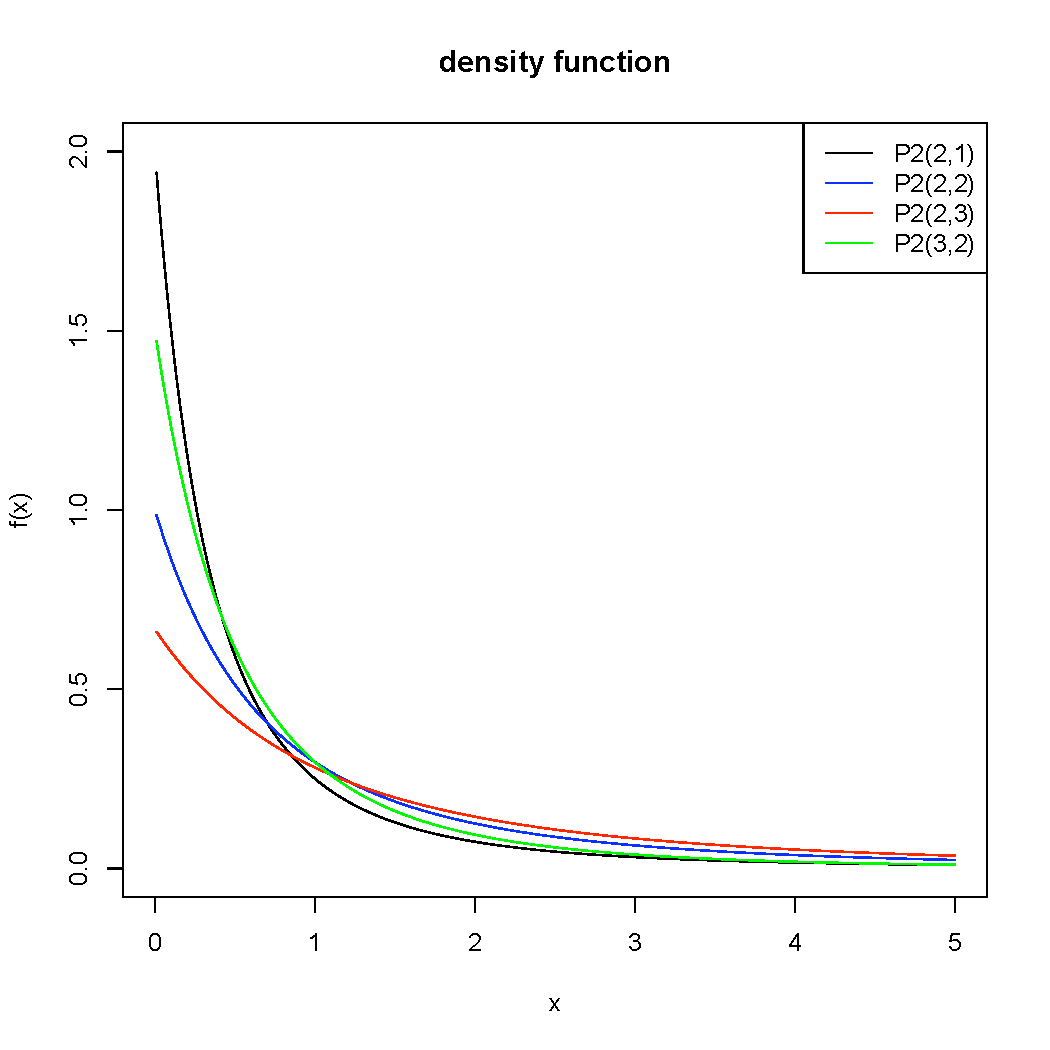
\includegraphics[width=0.48\textwidth]{img/pareto2zoom}
  \end{center}
  \vspace{-20pt}  
  \caption{Density function for Pareto II distributions}
  \vspace{-20pt}  
\end{wrapfigure}
The Pareto type II distribution $\mcal Pa_{II}(\mu, \sigma, \alpha)$ is characterized by this survival function
$$
\bar F(x) = \left(1+\frac{x-\mu}{\sigma}\right)^{-\alpha},
$$
where $x>\mu$ and $\sigma,\alpha>0$. Again $\alpha$ is the shape parameter, while $\mu$ is the location parameter. We can derive the density from this definition:
$$
f(x)= \frac{\alpha}{\sigma}  \left(1+\frac{x-\mu}{\sigma}\right)^{-\alpha-1},
$$
for $x>\mu$. We retrieve the Pareto I distribution with $\mu=\sigma$, i.e. if $X$ follows a Pareto I distribution then $\mu-\sigma+X$ follows a Pareto II distribution. The Pareto II is sometimes called the American Pareto distribution.

\subsubsection{Pareto III}
\begin{wrapfigure}{r}{0.5\textwidth}
  \vspace{-20pt}
  \begin{center}
    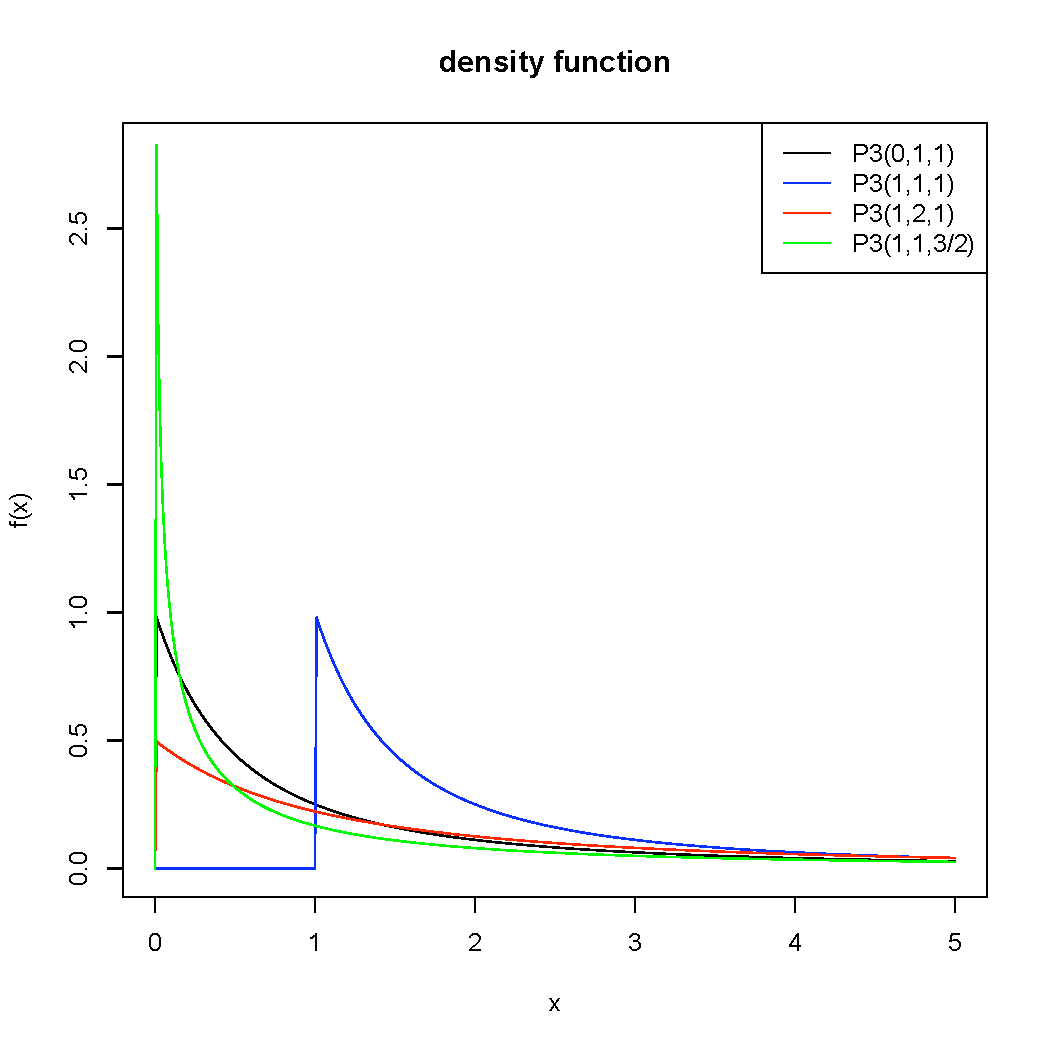
\includegraphics[width=0.48\textwidth]{img/pareto3zoom}
  \end{center}
  \vspace{-20pt}  
  \caption{Density function for Pareto III distributions}
  \vspace{-20pt}  
\end{wrapfigure}
A similar distribution to the type II distribution is the Pareto type III $\mcal Pa_{III}(\mu, \sigma, \gamma)$ distribution defined as
$$
\bar F(x)  = \left(1+\left(\frac{x-\mu}{\sigma}\right)^{\frac{1}{\gamma}}\right)^{-1},
$$
where $x>\mu$, $\gamma,\sigma>0$. The $\gamma$ parameter is called the index of inequality, and in the special case of $\mu=0$, it is the Gini index of inequality. The density function is given by
$$
f(x)  = \frac{1}{\gamma\sigma} \left(\frac{x-\mu}{\sigma}\right)^{\frac{1}{\gamma}-1} \left(1+\left(\frac{x-\mu}{\sigma}\right)^{\frac{1}{\gamma}}\right)^{-2},
$$
where $x>\mu$. The Pareto III is not a generalisation of the Pareto II distribution, but from these two distribution we can derive more general models. It can be seen as the following transformation $\mu+\sigma Z^\gamma$, where $Z$ is a Pareto II $\mcal Pa_{II}(0, 1, 1)$.

\subsubsection{Pareto IV}
\begin{wrapfigure}{r}{0.5\textwidth}
  \vspace{-20pt}
  \begin{center}
    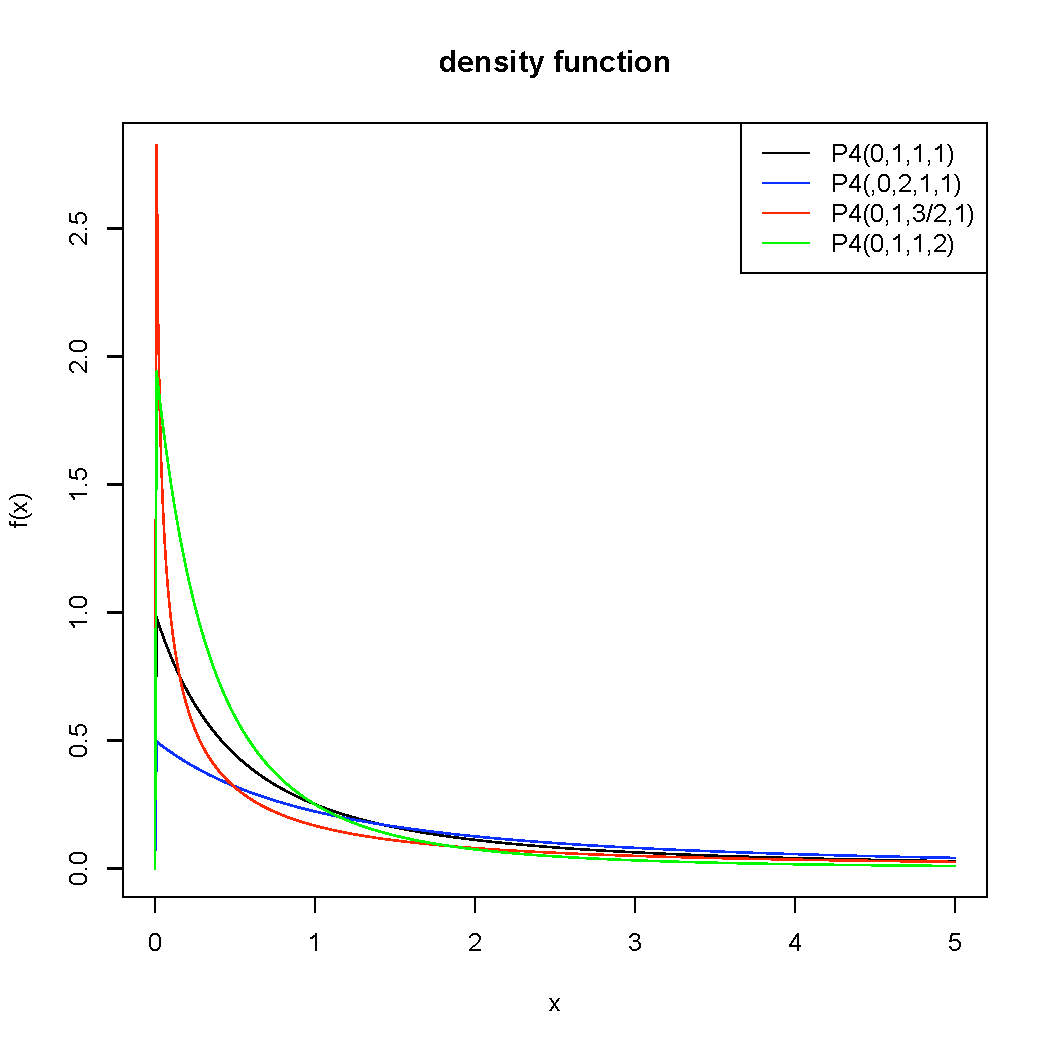
\includegraphics[width=0.48\textwidth]{img/pareto4zoom}
  \end{center}
  \vspace{-20pt}  
  \caption{Density function for Pareto IV distributions}
  \vspace{-20pt}  
\end{wrapfigure}
The Pareto type IV $\mcal Pa_{IV}(\mu, \sigma, \gamma, \alpha)$ distribution is defined by
$$
\bar F(x)  = \left(1+\left(\frac{x-\mu}{\sigma}\right)^{\frac{1}{\gamma}}\right)^{-\alpha},
$$
where $x>\mu$ and $\alpha,\sigma, \gamma>0$. The associated density function is expressed as follows
$$
f(x) = \frac{\alpha}{\gamma\sigma} \left(\frac{x-\mu}{\sigma}\right)^{\frac{1}{\gamma}-1} \left(1+\left(\frac{x-\mu}{\sigma}\right)^{\frac{1}{\gamma}}\right)^{-\alpha-1}
$$
for $x>\mu$.

Quantile functions for Pareto distributions are listed in sub-section random generation.

The generalized Pareto used in extreme value theory due to \cite{pickands} has a limiting distribution with Pareto II $\mcal Pa_{II}(0, \sigma, \alpha)$, see chapter on EVT for details. Finally, the Feller-Pareto is a generalisation of the Pareto IV distribution, cf. next section.

\subsection{Properties}

\subsubsection{Equivalence}
It is easy to verify that if $X$ follows a Pareto I distribution $\mcal Pa_I(\sigma, \alpha)$, then $\log X$ follows a translated exponential distribution $\mcal T\mcal E(\sigma, \alpha ?)$.

The Pareto type III distribution is sometimes called the log-logistic distribution, since if $X$ has a logistic distribution then $e^X$ has a Pareto type III distribution with $\mu=0$.

\subsubsection{Moments}
Moments for the Pareto I distribution are given by 
$E(X) = \frac{\alpha \sigma}{\alpha-1}$ if $\alpha > 1$, $Var(X) = \frac{\alpha \sigma^2}{(\alpha-1)^2(\alpha-2)}$ and $E(X^\tau) = \tau \frac{\alpha}{\alpha-\tau}$ for $\alpha >\tau$ and $\sigma=1$.

Moments for the Pareto II, III can be derived from those of Pareto IV distribution, which are
$$
E(X^\tau) = \sigma^\tau \frac{\Gamma(1+\tau\gamma)\Gamma(\alpha-\tau\gamma)}{\Gamma(\alpha)},
$$
with $-1<\tau\gamma<\alpha$ and $\mu=0$.

\subsubsection{Convolution and sum}
The convolution (i.e. sum) of Pareto I distributions does not have any particular form but the product of Pareto I distributions does have a analytical form. 

If we consider of $n$ i.i.d. Pareto I $\mcal Pa_I(\sigma, \alpha)$ random variables, then the product $\Pi$ has the following density
$$
f_\Pi(x) = \frac{\alpha \left(\sigma \log(\frac{x-\sigma}{\sigma}) \right)^{n-1} \left(\frac{x}{\sigma}\right)^{-\alpha}  }{x \Gamma(n)},
$$
where $x>\sigma$.

If we consider only independent Pareto I distribution $\mcal Pa_I(\sigma_i, \alpha_i)$, then we have for the density of the product
$$
f_\Pi(x) = \sum_{i=1}^n\frac{\alpha_i}{\sigma} \left(\frac{x}{\sigma}\right)^{-\alpha_i-1} \prod_{k\neq i}\frac{\alpha_k}{\alpha_i-\alpha_k},
$$
where $x> \prod_{i=1}^n\sigma_i$.

Other Pareto distributions??



\subsubsection{Order statistics}
Let $(X_i)_i$ be a sample of Pareto distributions. We denote by $(X_{i:n})_i$ the associated order statistics, i.e. $X_{1:n}$ is the minimum and $X_{n:n}$ the maximum.

For Pareto I distribution, the $i$th order statistic has the following survival function
$$
\bar F_{X_{i:n}}(x) = \sum_{j=1}^i \left(1+\frac{x}{\sigma}\right)^{-\alpha(n-j+1)} \prod_{\stackrel{l=1}{l\neq i}}^{i}\frac{n-l+1}{l-j},
$$
where $x>0$. Furthermore moments are given by
$$
E(X_{i:n}^\tau) = \sigma^\tau \frac{n!}{(n-i)!} \frac{\Gamma(n-i+1-\tau\alpha^{-1})}{\Gamma(n+1-\tau\alpha^{-1})},
$$
for $\tau\in\mbb R$.

For Pareto II distribution, we get
$$
\bar F_{X_{i:n}}(x) = \sum_{j=1}^i \left(1+\frac{x-\mu}{\sigma}\right)^{-\alpha(n-j+1)} \prod_{\stackrel{l=1}{l\neq i}}^{i}\frac{n-l+1}{l-j},
$$
where $x>\mu$. Moments can be derived from those in the case of the Pareto I distribution using the fact $X_{i:n} = \mu-\sigma+Y_{i:n}$ with $Y_{i:n}$ order statistic for the Pareto I case.

For Pareto III distribution, the $i$th order statistic follows a Feller-Pareto $\mcal F\mcal Pa(\mu, \sigma, \gamma, i, n-i+1)$. Moments of order statistics can be obtained by using the transformation  of Pareto II random variable: we have $X_{i:n}=\mu+\sigma Z_{i:n}^\gamma$ follows a Pareto III distribution, where $Z$ is a Pareto II $\mcal Pa_{II}(0, 1, 1)$. Furthermore, we know the moments of the random variable $Z$:
$$
E(Z_{i:n}^\tau) = \frac{\Gamma(i+\tau)\Gamma(n-i+\tau+1)}{\Gamma(i)\Gamma(n-i+1)}
$$

The minimum of Pareto IV distributions still follows a Pareto IV distribution. Indeed if we consider $n$ independent random variables Pareto IV $\mcal Pa_{IV}(\mu, \sigma, \gamma, \alpha_i)$ distributed, we have
$$
\min(X_1,\dots,X_n)\sim \mcal Pa_{IV}\left(\mu, \sigma, \gamma, \sum_{i=1}^n\alpha_i\right).
$$
But the $i$th order statistic does not have a particular distribution. The intermediate order statistic can be approximated by the normal distibution with 
$$
X_{i:n} \underset{n\rightarrow +\infty}{\longrightarrow} \mcal N\left(F^{-1}\left(i/n\right),i/n\left(1-i/n\right)f^{-2}\left(F^{-1}\left(i/n\right)\right) n^{-1} \right)
$$
where $f$ and $F$ denotes respectively the density and the distribution function of the Pareto IV distribution.
Moments for the order statistics are computable from the moments of the minima since we have
$$
E(X_{i:n}^\tau) = \sum_{r=n-i+1}^n(-1)^{r-n+i-1} C_n^r C_{r-1}^{n-i} E(X_{1:r}^\tau).
$$
Since $X_{1:r}$ still follows a Pareto IV distribution $\mcal P_{IV}(\mu, \sigma, \gamma, r\alpha)$, we have
$$
E(X_{1:r}^\tau) = E((\mu+\sigma Z_{1:r})^\tau),
$$
where $Z_{1:r} \sim \mcal Pa_{IV}(0, 1, \gamma, r\alpha)$ and $E(Z_{1:r}^\tau)=\frac{\Gamma(1+\tau\gamma) \Gamma(r\alpha-\tau\gamma)}{\Gamma(r\alpha)}$.



\subsubsection{Truncation}
Let us denote by $X | X>x_0$ the random variable $X$ knowing that $X>x_0$. We have the following properties (with $x_0>\mu$):
\begin{itemize}
\item if $X\sim \mcal Pa_I(\sigma, \alpha)$ then $X | X>x_0\sim \mcal Pa_I(x_0, \alpha)$\footnote{In this case, the truncation is a rescaling. It comes from the lack of memory property of the log variable since the log variable follows an exponential distribution.}
\item if $X\sim \mcal Pa_{II}(\mu, \sigma, \alpha)$ then $X | X>x_0\sim \mcal Pa_I(x_0, \sigma+x_0-\mu, \alpha)$
\end{itemize}
More general distributions do not have any particular form.

\subsubsection{Record values}

\subsubsection{Geometric minimization}

\subsection{Estimation}
Estimation of the Pareto distribution in the context of actuarial science can be found in \cite{rytgaard}.

\subsubsection{Pareto I}
\cite{arnold83} notices that from a log transformation, the parameter estimation reduces to a problem for a translated exponentiallly distributed data. From this, we have the following maximum likelihood estimator for the Pareto I distribution
\begin{itemize}
\item $\hat \alpha_n = X_{1:n}$,
\item $\hat \sigma_n = \left[ \frac{1}{n} \sum_{i=1}^n \log\left(\frac{X_i}{X_{1:n}}\right) \right]^{-1}$,
\end{itemize}
where $(X_i)_{1\leq i\leq n}$ denotes a sample of i.i.d. Pareto variables. Those estimators are strongly consistent estimator of $\alpha$ and $\sigma$. Let us note that for these estimator we have better than the asymptotic normality (due to the maximum likelihoodness). The distributions for these two estimators are
respectively Pareto I and Gamma distribution:
\begin{itemize}
\item $\hat \alpha_n \sim \mcal P_I(\sigma, n\alpha)$,
\item $\hat \sigma_n^{-1} \sim \mcal G(n-1, (\alpha n)^{-1})$.
\end{itemize}
From this, we can see these estimators are biased, but we can derive unbiased estimators with minimum variance: 
\begin{itemize}
\item $\tilde \alpha_n = \frac{n-2}{n}\hat \alpha_n$,
\item $\tilde \sigma_n = \left[ 1 - \frac{1}{\hat \alpha_n} \right] \hat \sigma_n$.
\end{itemize}
Since those statistics $\tilde \alpha_n$ and $\tilde \sigma_n$ are sufficient, it is easy to find unbiased estimators of functions of these parameters $h(\alpha,\sigma)$ by plugging in $\tilde \alpha_n$ and $\tilde \sigma_n$ (i.e. $h(\tilde \alpha_n,\tilde \sigma_n)$).

However other estimations are possible, for instance we may use a least square regression on the Pareto chart (plot of $\log \bar F(x)$ against $\log x$). We can also estimate parameters by the method of moments by equalling the sample mean and minimum to corresponding theoretical moments. We get
\begin{itemize}
\item $\hat \alpha_n^M = \frac{n \bar X_n - X_{1:n}}{n (\bar X_n - X_{1:n})}$,
\item $\hat \sigma_n^M = \frac{n\hat \alpha_n^M-1}{n\hat \alpha_n^M} X_{1:n}$,
\end{itemize}
where we assume a finite expectation (i.e. $\alpha>1$).

Finally, we may also calibrate a Pareto I distribution with a quantile method. We numerically solve the system
$$
\left\{
\begin{array}{c}
p_1 = 1- \left(\frac{X_{\lfloor np_1\rfloor:n}}{\sigma}\right)^\alpha\\
p_2 = 1- \left(\frac{X_{\lfloor np_2\rfloor:n}}{\sigma}\right)^\alpha
\end{array}
\right. ,
$$
for two given probabilities $p_1, p_2$.

\subsubsection{Pareto II-III-IV}
Estimation of parameters for Pareto II, III and IV are more difficult. If we write the log-likelihood for a sample $(X_i)_{1\leq i\leq n}$ Pareto IV distributed, we have
$$
\log \mcal L(\mu, \sigma, \gamma, \alpha) = \left(\frac{1}{\gamma}-1\right)\sum_{i=1}^n\log \left( \frac{x_i-\mu}{\sigma} \right) - (\alpha+1)\sum_{i=1}^n \log \left(1+ \left(\frac{x_i-\mu}{\sigma}\right)^{\frac{1}{\gamma}} \right) -n\log \gamma-n\log\sigma+n\log \alpha ,
$$
with the constraint that $\forall 1\leq i \leq n, x_i>\mu$. Since the log-likelihood is null when $x_{1:n}\leq\mu$ and a decreasing function of $\mu$ otherwise the maximum likelihood estimator of $\mu$ is the minimum  $\hat \mu =X_{1:n}$. 

Then if we substract $\hat \mu$ to all observations, we get the following the log-likelihood
$$
\log \mcal L(\sigma, \gamma, \alpha) = \left(\frac{1}{\gamma}-1\right)\sum_{i=1}^n\log \left( \frac{x_i}{\sigma} \right) - (\alpha+1)\sum_{i=1}^n \log \left(1+ \left(\frac{x_i}{\sigma}\right)^{\frac{1}{\gamma}} \right) -n\log \gamma-n\log\sigma+n\log \alpha,
$$
which can be maximised numerically. Since there are no close form for estimators of $\sigma, \gamma, \alpha$, we do not know their distributions, but they are asymptotically normal.

We may also use the method of moments, where again $\hat \mu$ is $X_{1:n}$. Substracting this value to all observations, we use the expression of moments above to have three equations. Finally solve the system numerically. A similar scheme can be used to estimate parameters with quantiles.



\subsection{Random generation}
It is very easy to generate Pareto random variate using the inverse function method. Quantiles function can be easily calculated
\begin{itemize}
\item for $\mcal P_{I}(\sigma, \alpha)$ distribution, $F^{-1}(u) = \sigma(1-u)^{\frac{-1}{\alpha}}$,
\item for $\mcal P_{II}(\mu,\sigma, \alpha)$ distribution, $F^{-1}(u) = \sigma\left[(1-u)^{\frac{-1}{\alpha}} -1\right]+\mu$,
\item for $\mcal P_{III}(\mu,\sigma, \gamma)$ distribution, $F^{-1}(u) = \sigma\left[(1-u)^{-1} -1\right]^\gamma+\mu$,
\item for $\mcal P_{IV}(\mu,\sigma, \alpha)$ distribution, $F^{-1}(u) = \sigma\left[(1-u)^{\frac{-1}{\alpha}} -1\right]^\gamma+\mu$.
\end{itemize}
Therefore algorithms for random generation are simply
\begin{itemize}
\item for $\mcal P_{I}(\sigma, \alpha)$ distribution, $F^{-1}(u) = \sigma U^{\frac{-1}{\alpha}}$,
\item for $\mcal P_{II}(\mu,\sigma, \alpha)$ distribution, $F^{-1}(u) = \sigma\left[U^{\frac{-1}{\alpha}} -1\right]+\mu$,
\item for $\mcal P_{III}(\mu,\sigma, \gamma)$ distribution, $F^{-1}(u) = \sigma\left[U^{-1} -1\right]^\gamma+\mu$,
\item for $\mcal P_{IV}(\mu,\sigma, \alpha)$ distribution, $F^{-1}(u) = \sigma\left[U^{\frac{-1}{\alpha}} -1\right]^\gamma+\mu$,
\end{itemize}
where $U$ is an uniform random variate.


\subsection{Applications}
From wikipedia, we get the following possible applications of the Pareto distributions:
\begin{itemize}
\item the sizes of human settlements (few cities, many hamlets/villages),
\item file size distribution of Internet traffic which uses the TCP protocol (many smaller files, few larger ones),
\item clusters of Bose-Einstein condensate near absolute zero,
\item the values of oil reserves in oil fields (a few large fields, many small fields),
\item the length distribution in jobs assigned supercomputers (a few large ones, many small ones),
\item the standardized price returns on individual stocks,
\item sizes of sand particles,
\item sizes of meteorites,
\item numbers of species per genus (There is subjectivity involved: The tendency to divide a genus into two or more increases with the number of species in it),
\item areas burnt in forest fires,
\item severity of large casualty losses for certain lines of business such as general liability, commercial auto, and workers compensation.
\end{itemize}
In the litterature, \cite{arnold83} uses the Pareto distribution to model the income of an individual and \cite{froot} apply the Pareto distribution as the severity distribution in a context of catastrophe reinsurance. Here are just a few applications, many other applications can be listed.

%%%%%%%%%%%%%%%%%%%%%%%%%%%%%%%%%%%%%%%%%%%%%%
\section{Feller-Pareto distribution}
\subsection{Characterization}
As described in \cite{arnold83}, the Feller-Pareto distribution is the distribution of
$$
X = \mu +\sigma\left(\frac{U}{V}\right)^\gamma,
$$
where $U$ and $V$ are independent gamma variables ($\mcal G(\delta_1,1)$ and $\mcal G(\delta_2,1)$ respectively). Let us note that the ratio of these two variables follows a beta distribution of the second kind.
In term of distribution function, using the transformation of the beta variable, we get
$$
F(x) = \frac{\beta\left(\delta_1,\delta_2, \frac{y}{1+y}\right)}{\beta(\delta_1,\delta_2)} \txtm{with} y = \left(\frac{x-\mu}{\sigma}\right)^{\frac{1}{\gamma}},
$$
with $x\geq \mu$, $\beta(.,.)$ denotes the beta function and $\beta(.,.,.)$ the incomplete beta function.

We have the following density for the Feller-Pareto distribution $\mcal F\mcal P(\mu,\sigma,\gamma,\delta_1,\delta_2)$ :
$$
f(x) = \frac{(\frac{x-\mu}{\sigma})^{\frac{\delta_2}{\gamma}-1}}{\gamma \beta(\delta_1, \delta_2) x (1+(\frac{x-\mu}{\sigma})^{\frac{1}{\gamma}})^{\delta_1 + \delta_2}},
$$
where $x\geq\mu$. Let $y$ be $\frac{x-\mu}{\sigma}$, the previous expression can be rewritten as
$$
f(x) =  \frac{1 }{ \gamma \beta(\delta_1, \delta_2)   }
\left(\frac{ y^{\frac{1}{\gamma}} }{ 1+y^{\frac{1}{\gamma}} } \right)^{\delta_2}  
\left(1- \frac{ y^{\frac{1}{\gamma}} }{ 1+y^{\frac{1}{\gamma}} } \right)^{\delta_1}
 \frac{ 1 }{  x y },
$$
for $x\geq\mu$. In this expression, we see more clearly the link with the beta distribution as well as the transformation of the variable $\frac{U}{V}$.

There is a lot of special cases to the Feller-Pareto distribution $\mcal F\mcal P(\mu,\sigma,\gamma,\delta_1,\delta_2)$. When $\mu=0$, we retrieve the transformed beta distribution\footnote{sometimes called the generalized beta distribution of the second kind.} of \cite{klugman} and if in addition $\gamma=1$, we get the ``generalized'' Pareto distribution\footnote{which has nothing to do with the generalized Pareto distribution of the extreme value theory.} (as defined by \cite{klugman}).

Finally the Pareto IV distribution is obtained with $\delta_1=1$. Therefore we have the following equivalences
\begin{itemize}
\item $\mcal P_I(\sigma,\alpha) =  \mcal F\mcal P(\sigma,\sigma,1,1,\alpha)$,
\item $\mcal P_{II}(\mu,\sigma,\alpha) =  \mcal F\mcal P(\mu,\sigma,1,1,\alpha)$,
\item $\mcal P_{III}(\mu,\sigma,\gamma) =  \mcal F\mcal P(\mu,\sigma,\gamma,1,1)$,
\item $\mcal P_{IV}(\mu,\sigma,\gamma,\alpha) =  \mcal F\mcal P(\mu,\sigma,\gamma,1,\alpha)$.
\end{itemize}

\subsection{Properties}
When $\mu=0$, raw moments are given by
$$
E(X^r) = \sigma^r \frac{\Gamma(\delta_1+r\gamma)
\Gamma(\delta_2-r\gamma)}{\Gamma(\delta_1)\Gamma(\delta_2)},
$$
for $-\frac{\delta_1}{\gamma}\leq r\leq \frac{\delta_2}{\gamma}$.

\subsection{Estimation}
NEED REFERENCE
\subsection{Random generation}
Once we have simulated a beta I distribution $B$, we get a beta II distribution\footnote{We can also use two gamma variables to get the beta II variable.} with $\tilde B = \frac{B}{1-B}$. Finally we shift, scale and take the power $X = \mu +\sigma\left(\tilde B\right)^\gamma$ to get a Feller-Pareto random variable.  

\subsection{Applications}
NEED REFERENCE


%%%%%%%%%%%%%%%%%%%%%%%%%%%%%%%%%%%%%%%%%%%%%%
\newpage
\section{Inverse Pareto}
\subsection{Characterization}
\begin{wrapfigure}{r}{0.5\textwidth}
  \vspace{-40pt}
  \begin{center}
    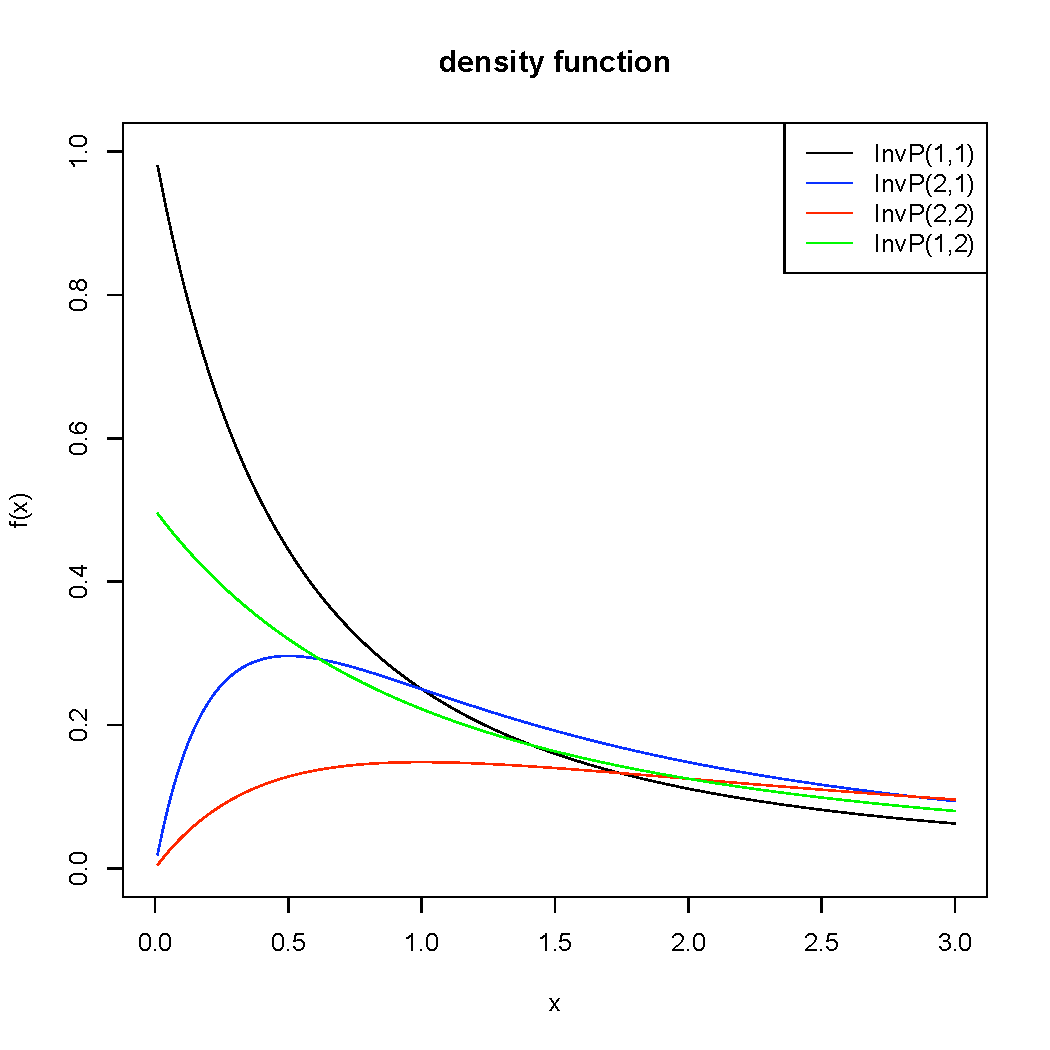
\includegraphics[width=0.48\textwidth]{img/invparetozoom}
  \end{center}
  \vspace{-20pt}  
  \caption{Density function for inverse Pareto distributions}
  \vspace{-20pt}  
\end{wrapfigure}
From the Feller-Pareto distribution, we get the inverse Pareto distribution with $\mu=0$,
$\delta_1=1$ and $\gamma=1$. Thus the density is
$$
f(x) =  \frac{1 }{ \beta(1, \delta_2)   }
\left(\frac{ \frac{x}{\sigma} }{ 1+\frac{x}{\sigma} } \right)^{\delta_2}  
\frac{ 1 }{ 1+\frac{x}{\sigma} } \frac{ 1 }{  \frac{x}{\sigma} },
$$
It can be rewritten as the density
$$
f(x) =  \frac{\tau\lambda x^{\tau-1}}{(x+\lambda)^{\tau+1}} 
$$
which implies the following distribution function
$$
F(x) = \left( \frac{x}{x+\lambda}\right)^\tau,
$$
for $x\geq 0$.
Let us note this is the distribution of $\frac{1}{X}$ when $X$ is Pareto II.

\subsection{Properties}
The expectation of the inverse Pareto distribution is $E(X) = \frac{\lambda\Gamma(\tau+1)}{\Gamma(\tau)}$, but the variance does not exist.

\subsection{Estimation}
NEED REFERENCE
\subsection{Random generation}
Simply inverse a Pareto II variable.

\subsection{Applications}
NEED REFERENCE

%%%%%%%%%%%%%%%%%%%%%%%%%%%%%%%%%%%%%%%%%%%%%%
\section{Generalized Pareto distribution}\label{GPD}
\subsection{Characterization}
\begin{wrapfigure}{r}{0.5\textwidth}
  \vspace{-50pt}
  \begin{center}
    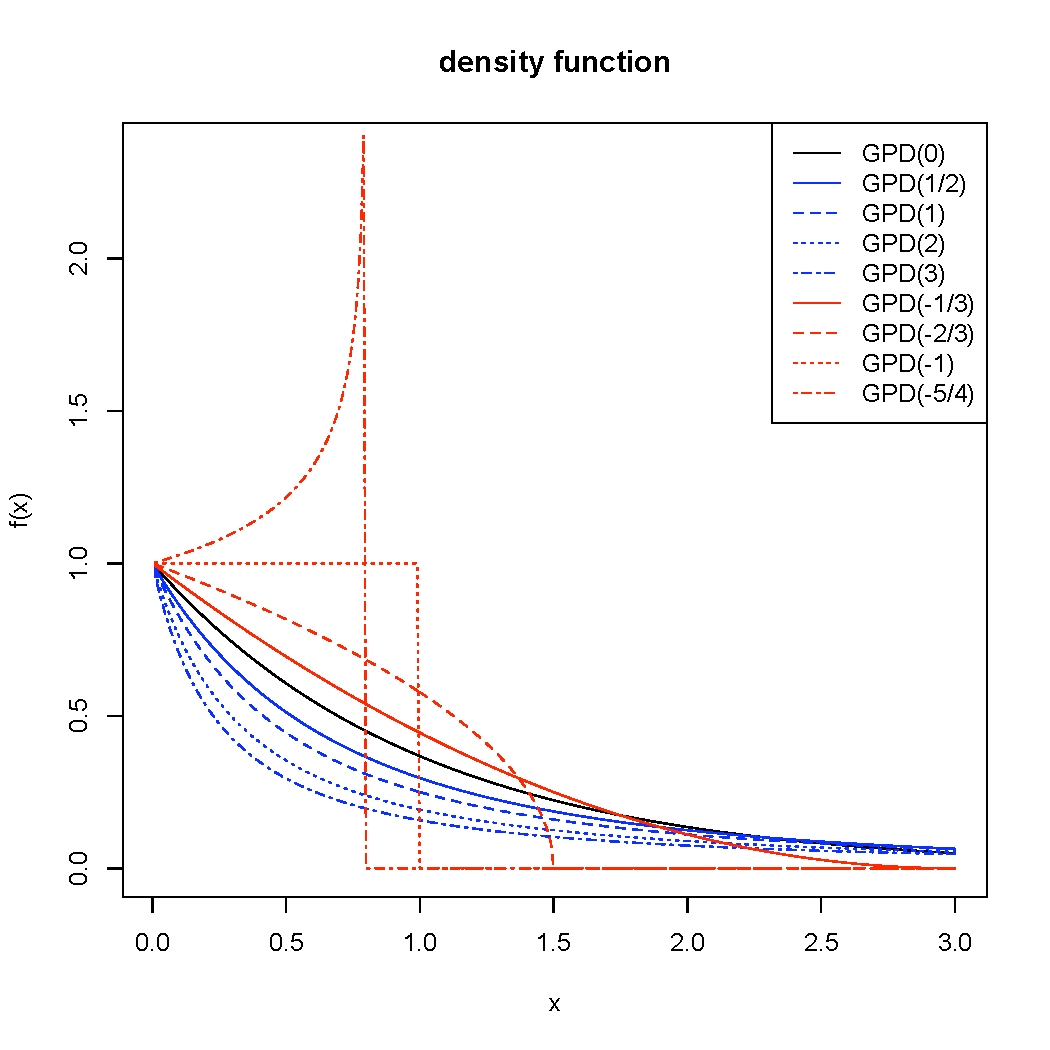
\includegraphics[width=0.48\textwidth]{img/gpdzoom}
  \end{center}
  \vspace{-20pt}  
  \caption{Density function for standard generalized Pareto distributions}
  \vspace{-20pt}  
\end{wrapfigure}

The generalized Pareto distribution was introduced in \cite{tve} in the context of extreme value theory.

We first define the standard generalized Pareto distribution by the following distribution function
$$
F(x) = \left\{
\begin{array}{ll}
1- \left(1+\xi x\right)^{-\frac{1}{\xi}} & \txtm{if} \xi \neq 0\\
1-e^{-x} & \txtm{if} \xi=0\\
\end{array}
\right. ,
$$
where $x\in\mbb R_+$ if $\xi\geq 0$ and $x\in\left[0, -\frac{1}{\xi}\right]$ otherwise. This distribution function is generally denoted by $G_\xi$.  

We can see the impact of the shape parameter $\xi$ on the figure on the right. The case where $\xi=0$ can be seen as a limiting case of $G_\xi$ when $\xi\rightarrow 0$.

To get the ``full'' generalized Pareto distribution, we introduce a scale $\beta$ and a location parameter $\mu$. We get
$$
F(x) = \left\{
\begin{array}{ll}
1- \left(1+\xi \frac{x-\nu}{\beta}\right)^{-\frac{1}{\xi}} & \txtm{if} \xi > 0\\
1-e^{-\frac{x-\nu}{\beta}} & \txtm{if} \xi=0\\
1- \left(1+\xi \frac{x-\nu}{\beta}\right)^{-\frac{1}{\xi}} & \txtm{if} \xi < 0\\
\end{array}
\right. ,
$$
where $x$ lies in $[\nu,+\infty[$, $[\nu,+\infty[$ and $\left[\nu, \nu-\frac{\beta}{\xi}\right]$ respectively. We denote it by $G_{\xi,\nu,\beta}(x)$ (which is simply $G_{\xi}(\frac{x-\nu}{\beta})$). Let us note when $\xi>0$, we have a Pareto II distribution, when $\xi=0$ a shifted exponential distribution and when $\xi<0$ a generalized beta I distribution.

From these expression, we can derive a density function for the generalized Pareto distribution
$$
f(x) = \left\{
\begin{array}{ll}
\frac{1}{\beta} \left(1+\xi \frac{x-\nu}{\beta}\right)^{-\frac{1}{\xi}-1} & \txtm{if} \xi > 0\\
\frac{1}{\beta} e^{-\frac{x-\nu}{\beta}} & \txtm{if} \xi=0\\
\frac{1}{\beta} \left(1-(-\xi) \frac{x-\nu}{\beta}\right)^{\frac{1}{-\xi}-1} & \txtm{if} \xi < 0\\
\end{array}
\right. ,
$$
for $x$ in the same supports as above. 


\subsection{Properties}
For a generalized Pareto distribution $G_{\xi,0,\beta}$, we have results on raw moments (for simplicity $\nu=0$). The expectation $E(X)$ is finite if and only if $\xi<1$. In this case we have
\begin{align*}
E\left(\left(1+ \frac{\xi}{\beta}X\right)^{-r}\right) = \frac{1}{1+\xi r}, \txtm{for} r>-\frac{1}{\xi}\\
E\left(\left(\log\left(1+ \frac{\xi}{\beta}X\right)\right)^k\right) = \xi^k k!, \txtm{for} k \in\mbb N\\
E\left(X \bar F(X)^r \right) = \frac{\beta}{(r+1-\xi)(r+1)}, \txtm{for} \frac{r+1}{|\xi|}>0\\
E\left(X^k\right) = \frac{\beta^k}{\xi^{k+1}} \frac{\Gamma(\xi^{-1}-k)}{\Gamma(1+\xi^{-1})} k!, \txtm{for} \xi <\frac{1}{k},
\end{align*}
see \cite{tve} for details.

If $X$ follows a generalized Pareto distribution $GPD(\xi,0,\beta)$, then the treshold excess random variable $X-u| X>u$ still follows a generalized Pareto distribution $GPD(\xi,0,\beta+\xi u)$. Let $F_u$ be the distribution function of $X-u| X>u$.
We have $F$ is in the maximum domain of attraction $H_\xi$ if and only if 
$$
\underset{u\rightarrow x_f}{\lim} \underset{0<x<x_f-u}{\sup}  \left|F_u(x) - G_{\xi,0,\beta(u)}(x)  \right| = 0,
$$
where $\beta$ is a positive function. This makes the link between the generalized Pareto distribution and the generalized extreme value distribution.


\subsection{Estimation}
In this sub-section, we assume $\nu=0$.

\subsubsection{Peak Over a Treshold}
We briefly present the Peak Over a Treshold (POT) method to fit the generalized Pareto distribution. Let $(X_i)_{1\leq i\leq n}$ an i.i.d. sample whose distribution function belongs to a maximum domain of attraction  $H_\xi$. For a deterministic treshold $u>0$, we define the number of exceedances by
$$
N_u %=\card \Delta_u
= \card(1\leq i\leq n, X_i>u),
$$
with the corresponding excesses $(Y_i)_{1\leq i \leq N_u}$. We want to fit the excess distribution function $F_u$ with the GPD distribution function $G_{\xi,0,\beta(u)}$.

First we can use the linearity of the mean excess function
$$
E(X-u | X>u) = \frac{\beta+\xi u}{1-\xi},
$$
for a given $u$. This can be estimated by the empirical mean of the sample $(Y_i)_{1\leq i \leq N_u}$. \cite{tve} warn us about the difficulty of chosing $u$, since they are many $u$ for wich the plot of 
$(u, \bar Y_{N_u})$.

Once we find the treshold $u$, we can use conditional likelihood estimation on sample $(Y_i)_{1\leq i \leq N_u}$. Let $\tau$ be $ -\xi/\beta$. However we can also use a linear regression to fit the shape and the scale parameter.


\subsubsection{Maximum likelihood estimation}
Maximum likelihood estimators of $\xi$ and $\beta$ are solutions of the system
$$
\left\{
\begin{array}{l}
 \left(\frac{1}{\xi}+1\right)\sum\limits_{i=1}^n \frac{\xi X_i}{\beta^2+\beta \xi X_i} = \frac{n}{\beta}\\
 \frac{1}{\xi^2}\sum\limits_{i=1}^n\log\left(1+\frac{\xi}{\beta}X_i\right) = (\frac{1}{\xi}+1)\sum\limits_{i=1}^n\frac{X_i}{\beta+\xi X_i}
 \end{array}
 \right. ,
$$
but the system may be instable for $\xi\leq-1/2$. When $\xi>1/2$, we have some asymptotical properties of maximum likelihood estimators $\hat \xi$ and $\hat \beta$:
$$
\sqrt{n}\left(\hat\xi -\xi, \frac{\hat\beta}{\beta}-1\right) \stackrel{\mcal L}{\longrightarrow} \mcal N(0,M^{-1}),
$$
where the variance/covariance matrix for the bivariate normal distribution is
$$
M^{-1} = (1+\xi)\left(
\begin{array}{cc}
1+\xi & 1\\
1 & 2
\end{array}
\right) .
$$
Let us note that if we estimate a $\xi$ as zero, then we can try to fit a shifted exponential distribution.

\subsubsection{Method of moments}
From the properties, we know the theoretical expression of $E(X)$ and $E\left(X \bar F(X) \right)$. From wich we get the relation 
$$
\beta = \frac{2E(X)E\left(X \bar F(X) \right)}{E(X)-2E\left(X \bar F(X) \right)} \txtm{and} \xi = 2-\frac{E(X)}{E(X)-2E\left(X \bar F(X) \right)}.
$$
We simply replace $E(X)$ and $E\left(X \bar F(X) \right)$ by the empirical estimators.

\subsection{Random generation}
We have an explicit expression for the quantile function
$$
F^{-1}(u) = \left\{
\begin{array}{ll}
\nu+\frac{\sigma}{\xi}((1-u)^{-\xi}-1) & \txtm{if} \xi \neq 0\\
\nu-\sigma\log(1-u) & \txtm{if} \xi=0\\
\end{array}
\right.,
$$
thus we can use the inversion function method to generate GPD variables.

\subsection{Applications}
The main application of the generalized Pareto distribution is the extreme value theory, since there exists a link between the generalized Pareto distribution and the generalized extreme value distribution. Typical applications are modeling flood in hydrology, natural disaster in insurance and asset returns in finance.

%%%%%%%%%%%%%%%%%%%%%%%%%%%%%%%%%%%%%%%%%%%%%%
\section{Burr distribution}
\subsection{Characterization}
\begin{wrapfigure}{r}{0.5\textwidth}
  \vspace{-40pt}
  \begin{center}
    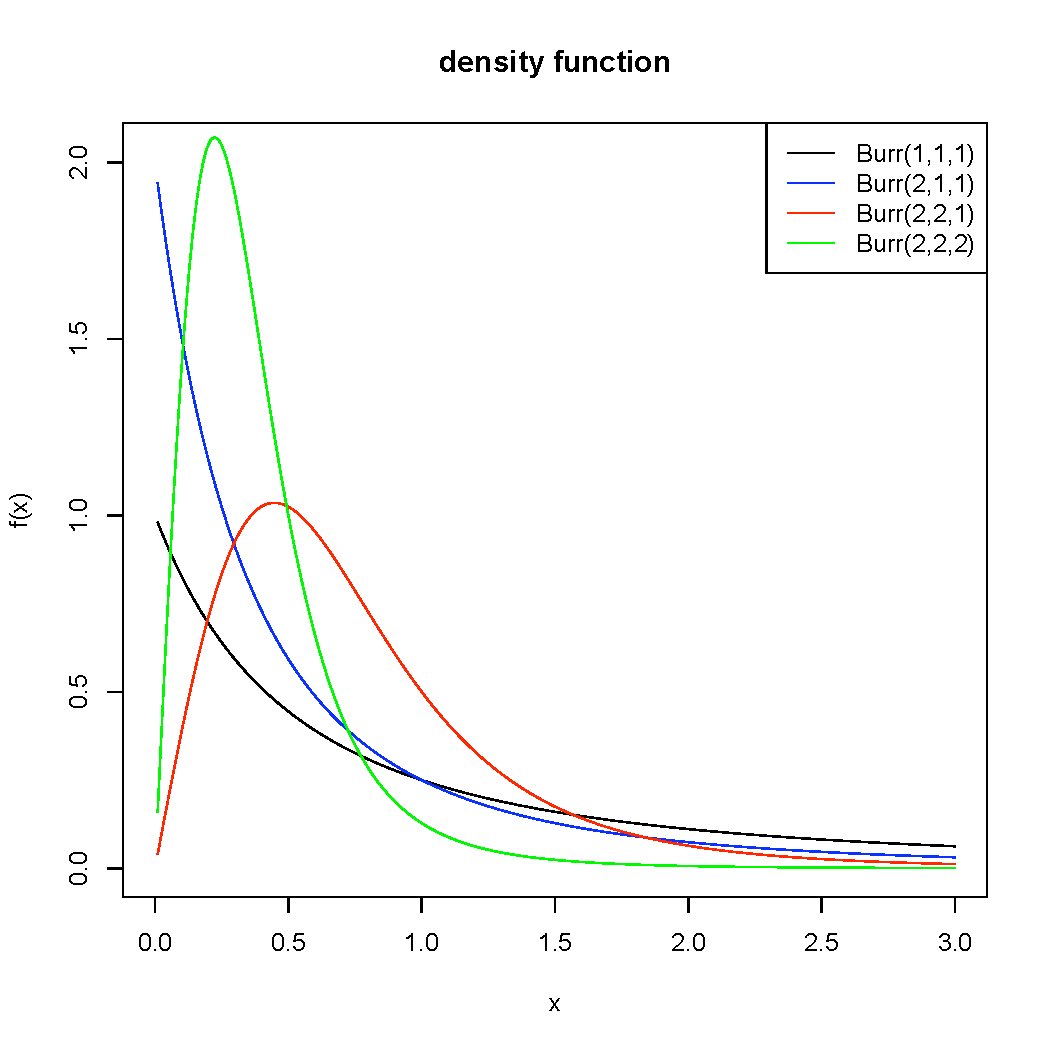
\includegraphics[width=0.48\textwidth]{img/burrzoom}
  \end{center}
  \vspace{-20pt}  
  \caption{Density function for Burr distributions}
  \vspace{-20pt}  
\end{wrapfigure}
The Burr distribution is defined by the following density
$$
f(x) =\frac{\alpha\tau}{\lambda} \frac{  (x/\lambda)^{\tau-1}}{(1+(x/\lambda)^\tau)^{\alpha+1}}
$$
where $x\geq0$, $\lambda$ the scale parameter and $\alpha,\tau>0$ the shape parameters. 
Its distribution function is given by
$$
F(x) = 1-\left(\frac{\lambda^\tau}{\lambda^\tau+x^\tau}\right)^{\alpha},
$$
for $x\geq 0$.
In a slightly different rewritten form, we recognise the Pareto IV distribution
$$
\bar F(x) = \left(1+\left(\frac{x}{\lambda}\right)^\tau\right)^{-\alpha},
$$
with a zero location parameter.

\subsection{Properties}
The raw moment of the Burr distribution is given by 
$$
E(X^r) = \lambda^r\frac{\Gamma(1+\frac{r}{\tau})\Gamma(\alpha-\frac{r}{\tau})}{\Gamma(\alpha)},
$$
hence the expectation and the variance are 
$$
E(X) = \lambda\frac{\Gamma(1+\frac{1}{\tau})\Gamma(\alpha-\frac{1}{\tau})}{\Gamma(\alpha)} \txtm{and}
Var(X) = \lambda^2\frac{\Gamma(1+\frac{2}{\tau})\Gamma(\alpha-\frac{2}{\tau})}{\Gamma(\alpha)} -\left(\lambda\frac{\Gamma(1+\frac{1}{\tau})\Gamma(\alpha-\frac{1}{\tau})}{\Gamma(\alpha)}\right)^2.
$$

\subsection{Estimation}
Maximum likelihood estimators are solution of the system
$$
\left\{
\begin{array}{l}
\frac{n}{\alpha}=\sum\limits_{i=1}^n\log \left(1+ \left(\frac{X_i}{\lambda}\right)^\tau\right)\\
\frac{n}{\tau}=-\sum\limits_{i=1}^n\log \left(\frac{X_i}{\lambda}\right)
+\tau\frac{\alpha+1}{\lambda}\sum\limits_{i=1}^n \log \left(\frac{X_i}{\lambda}\right) \frac{X_i^\tau}{\lambda^\tau+X_i^\tau}\\
\frac{n}{\lambda} = -\frac{\tau-1}{\lambda}\sum\limits_{i=1}^n\frac{1}{X_i}
+\tau\frac{\alpha+1}{\lambda}\sum\limits_{i=1}^n\frac{1}{\lambda^\tau+X_i^\tau}
\end{array}
\right. ,
$$
which can be solved numerically.

\subsection{Random generation}
From the quantile function $F^{-1}(u) = \lambda((1-u)^{\frac{1}{\alpha}} -1 )^{\frac{1}{\tau}}$, it is easy to generate Burr random variate with $\lambda(U^{\frac{1}{\alpha}} -1 )^{\frac{1}{\tau}}$ where $U$ is a uniform variable.

\subsection{Applications}
NEED REFERENCE

%%%%%%%%%%%%%%%%%%%%%%%%%%%%%%%%%%%%%%%%%%%%%%
\newpage
\section{Inverse Burr distribution}
\subsection{Characterization}
\begin{wrapfigure}{r}{0.5\textwidth}
  \vspace{-40pt}
  \begin{center}
    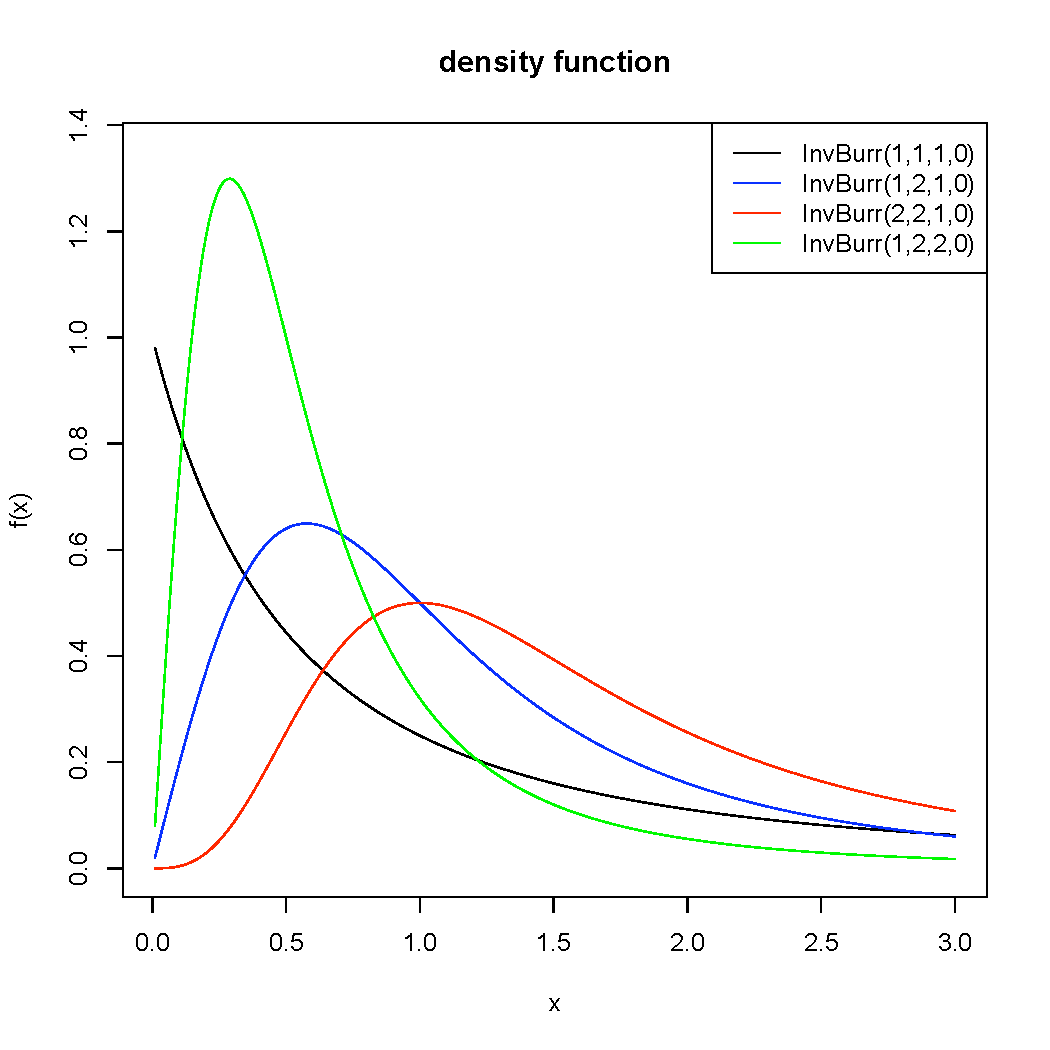
\includegraphics[width=0.48\textwidth]{img/invburrzoom}
  \end{center}
  \vspace{-20pt}  
  \caption{Density function for inverse Burr distributions}
  \vspace{-20pt}  
\end{wrapfigure}
The inverse Burr distribution (also called the Dagum distribution) is a special case of the Feller Pareto distribution $\mcal F\mcal P$ with $\delta_2=1$. That is to say the density is given by
$$
f(x) = \frac{\alpha\gamma}{\sigma} \frac{\left(\frac{x-\mu}{\sigma}\right)^{\alpha\gamma-1}}{\left(1+\left(\frac{x-\mu}{\sigma}\right)^{\alpha}\right)^{\gamma+1}},
$$
where $x\leq \mu$, $\mu$ the location parameter, $\sigma $ the scale parameter and $\alpha,\gamma$ the shape parameters. \cite{klugman} defines the inverse Burr distribution with $\mu=0$, 
%$$
%f(x) = \frac{\alpha\gamma}{\beta} \frac{\left(\frac{x}{\beta}\right)^{\alpha\gamma-1}}{\left(1+\left(\frac{x}{\beta}\right)^{\alpha}\right)^{\gamma+1}},
%$$
since this book deals with insurance loss distributions. In this expression, it is not so obvious that this is the inverse Burr distribution and not the Burr distribution. But the density can be rewritten as
$$
f(x) = \frac{\alpha\gamma}{\sigma} \frac{\left(\frac{\sigma}{x-\mu}\right)^{\alpha+1}}{\left(\left(\frac{\sigma}{x-\mu}\right)^{\alpha}+1\right)^{\gamma+1}},
$$
From this, the distribution function can be derived to 
$$
F(x) =\left(\frac{1}{\left(\frac{\sigma}{x-\mu}\right)^\alpha+1}\right)^{\gamma},
$$
for $x\geq \mu$. Here it is also clearer that this is the inverse Burr distribution since we notice the survival function of the Burr distribution taken in $\frac{1}{x}$. We denotes the inverse Burr distribution by $\mcal I\mcal B(\gamma,\alpha,\beta,\mu)$.

\subsection{Properties}
The raw moments of the inverse Burr distribution are given by
$$
E(X^r) = \sigma^r\frac{\Gamma(\gamma+\frac{r}{\alpha})\Gamma(1-\frac{r}{\alpha})}{\Gamma(\gamma)},
$$
when $\mu=0$ and $\alpha>r$. Thus the expectation and the variance are
$$
E(X) = \mu+\sigma\frac{\Gamma(\gamma+\frac{1}{\alpha})\Gamma(1-\frac{1}{\alpha})}{\Gamma(\gamma)}
$$
and 
$$
Var(X) = \sigma^2\frac{\Gamma(\gamma+\frac{2}{\alpha})\Gamma(1-\frac{2}{\alpha})}{\Gamma(\gamma)}-\sigma^2\frac{\Gamma^2(\gamma+\frac{1}{\alpha})\Gamma^2(1-\frac{1}{\alpha})}{\Gamma^2(\gamma)}
$$

Furthermore, we have the following special cases
\begin{itemize}
\item with $\gamma=\alpha$, we get the inverse paralogistic distribution,
\item with $\gamma=1$, we have the log logistic distribution,
\item with $\alpha=1$, this is the inverse Pareto distribution.
\end{itemize}

\subsection{Estimation}
The maximum likelihood estimator of $\mu$ is simply $\hat\mu=X_{1:n}$ for a sample $(X_i)_i$, then working on the transformed sample $Y_i=X_i-\hat\mu$, other maximum likelihood estimators are solutions of the system
$$
\left\{
\begin{array}{l}
\frac{n}{\gamma}=\sum\limits_{i=1}^n\log \left(1+ \left(\frac{\lambda}{Y_i}\right)^\alpha\right)\\
\frac{n}{\alpha}=-\sum\limits_{i=1}^n\log \left(\frac{\sigma}{Y_i}\right)
+(\gamma+1)\sum\limits_{i=1}^n  \log \left(\frac{\sigma}{Y_i}\right) \frac{\sigma^\alpha}{Y_i^\alpha+\sigma^\alpha}\\
\frac{n}{\sigma} = (\alpha+1)\sum\limits_{i=1}^n\frac{1}{Y_i+\sigma}
-\alpha\frac{\gamma+1}{\sigma}\sum\limits_{i=1}^n\frac{\sigma^\alpha}{Y_i^\alpha+\sigma^\alpha}
\end{array}
\right. ,
$$

\subsection{Random generation}
Since the quantile function is $F^{-1}(u) = \mu+\sigma^{-1}(u^{-\frac{1}{\gamma}}-1)^{-\frac{1}{\alpha}}$, we can use the inverse function method.

\subsection{Applications}
NEED REFERENCE

%%%%%%%%%%%%%%%%%%%%%%%%%%%%%%%%%%%%%%%%%%%%%%
\section{Beta type II distribution}
\subsection{Characterization}
There are many ways to characterize the beta type II distribution. First we can say it is the distribution of
$\frac{X}{1-X}$ when $X$ is beta I distributed. But this is also the distribution of the ratio $\frac{U}{V}$ when $U$ and $V$ are gamma distributed ($\mcal G(a,1)$ and $\mcal G(b,1)$ resp.).
The distribution function of the beta of the second distribution is given by
$$
F(x) = \frac{\beta(a,b,\frac{x}{1+x})}{\beta(a, b)},
$$
for $x\leq 0$. The main difference with the beta I distribution is that the beta II distribution takes values in $\mbb R_+$ and not $[0,1]$.

The density can be expressed as
$$
f(x) = \frac{x^{a-1}}{\beta(a, b) (1+x)^{a + b}},
$$
for $x\leq 0$. It is easier to see the transformation $\frac{x}{1-x}$ if we rewrite the density as
$$
f(x) = \left(\frac{x}{1+x}\right)^{a-1}\left(1-\frac{x}{1+x}\right)^{b-1}\frac{1}{\beta(a,b)(1+x)^2}.
$$
As already mentioned above, this is a special case of the Feller-Pareto distribution.
\subsection{Properties}
The expectation and the variance of the beta II are given by $E(X) = \frac{a}{b-1}$ and $Var(X) = \frac{a(a+b-1)}{(b-1)^2(b-2)}$ when $b>1$ and $b>2$.
Raw moments are expressed as follows 
$$
E(X^r) =  \frac{\Gamma(a+r)
\Gamma(b-r)}{\Gamma(a)\Gamma(b)},
$$
for $b>r$.

\subsection{Estimation}
Maximum likelihood estimators for $a$ and $b$ verify the system
$$
\left\{
\begin{array}{l}
\psi(a)-\psi(a+b) = \frac{1}{n}\sum\limits_{i=1}^n(\log(1+X_i)-\log(X_i))\\
\psi(b)-\psi(a+b) = \frac{1}{n}\sum\limits_{i=1}^n\log(1+X_i)\\
\end{array}
\right. ,
$$
where $\psi$ denotes the digamma function. We may also use the moment based estimators given by
$$
\tilde b = 2 + \frac{\bar X_n(\bar X_n+1)}{S_n^2} \txtm{and} \tilde a=(\tilde b-1)\bar X_n,
$$
which have the drawback that $\tilde b$ is always greater than 2.


\subsection{Random generation}
We can simply use the construction of the beta II, i.e. the ratio of $\frac{X}{1-X}$ when $X$ is beta I distributed. However we may also use the ratio of two gamma variables.

\subsection{Applications}
NEED REFERENCE

  
<<<<<<< .mine
%----------------------------------------------------------------------------------------------------------
% 	Copyright (c) 2009 R-forge 'distributions' Core Team, 
% 	
%	The following Sweave code is under the GNU Free Documentation License:
%      	Permission is granted to copy, distribute and/or modify this document
%      	under the terms of the GNU Free Documentation License, Version 1.3
%      	or any later version published by the Free Software Foundation;
%      	with no Invariant Sections, no Front-Cover Texts, and no Back-Cover Texts.
%
%      A copy of the license is included in the 'inst' directory of this package 
%      or on the web at http://www.gnu.org/licenses/licenses.html#FDL
%
%	After running Sweave, the following code could be compiled :
%	  - on windows with a Tex distribution such as miktex (http://miktex.org) 
%		and a front end Latex editor such as texniccenter (http://www.toolscenter.org)
%	  - on mac os with a Tex distribution such as TexLive and a front end Latex
%	  	editor such as Texshop (http://www.uoregon.edu/~koch/texshop/)
%	  - on linux with a Tex distribution such as teTex (http://www.tug.org/teTeX/)
%	  	and a front end Latex editor such as emacs (http://www.gnu.org/software/emacs/)
%
%----------------------------------------------------------------------------------------------------------

\chapter{Logistic distribution and related extensions}
%%%%%%%%%%%%%%%%%%%%%%%%%%%%%%%%%%%%%%%%%%%%%
\section{Logistic distribution}
\subsection{Characterization}
The logistic distribution is defined by the following distribution function
$$
F(x) = \frac{1}{1+e^{-\frac{x-\mu}{s}}},
$$
where $x\in\mbb R$, $\mu$ the location parameter and $s$ the scale parameter.
TODO
\subsection{Properties}
TODO
\subsection{Estimation}
TODO
\subsection{Random generation}
TODO
\subsection{Applications}

\section{Half logistic distribution}
\subsection{Characterization}
\subsection{Properties}
\subsection{Estimation}
\subsection{Random generation}
\subsection{Applications}

\section{Log logistic distribution}
\subsection{Characterization}
\subsection{Properties}
\subsection{Estimation}
\subsection{Random generation}
\subsection{Applications}

\section{Generalized log logistic  distribution}
\subsection{Characterization}
\subsection{Properties}
\subsection{Estimation}
\subsection{Random generation}
\subsection{Applications}

\section{Paralogisitic distribution}
\subsection{Characterization}
\subsection{Properties}
\subsection{Estimation}
\subsection{Random generation}
\subsection{Applications}

\section{Inverse paralogistic distribution}
\subsection{Characterization}
\subsection{Properties}
\subsection{Estimation}
\subsection{Random generation}
\subsection{Applications}

  
%----------------------------------------------------------------------------------------------------------
% 	Copyright (c) 2009 R-forge 'distributions' Core Team, 
% 	
%	The following Sweave code is under the GNU Free Documentation License:
%      	Permission is granted to copy, distribute and/or modify this document
%      	under the terms of the GNU Free Documentation License, Version 1.3
%      	or any later version published by the Free Software Foundation;
%      	with no Invariant Sections, no Front-Cover Texts, and no Back-Cover Texts.
%
%      A copy of the license is included in the 'inst' directory of this package 
%      or on the web at http://www.gnu.org/licenses/licenses.html#FDL
%
%	After running Sweave, the following code could be compiled :
%	  - on windows with a Tex distribution such as miktex (http://miktex.org) 
%		and a front end Latex editor such as texniccenter (http://www.toolscenter.org)
%	  - on mac os with a Tex distribution such as TexLive and a front end Latex
%	  	editor such as Texshop (http://www.uoregon.edu/~koch/texshop/)
%	  - on linux with a Tex distribution such as teTex (http://www.tug.org/teTeX/)
%	  	and a front end Latex editor such as emacs (http://www.gnu.org/software/emacs/)
%
%----------------------------------------------------------------------------------------------------------

\chapter{Extrem Value Theory distributions}
%%%%%%%%%%%%%%%%%%%%%%%%%%%%%%%%%%%%%%%%%%%%%
\section{Gumbel distribution}
\subsection{Characterization}
\begin{wrapfigure}{r}{0.5\textwidth}
  \vspace{-20pt}
  \begin{center}
    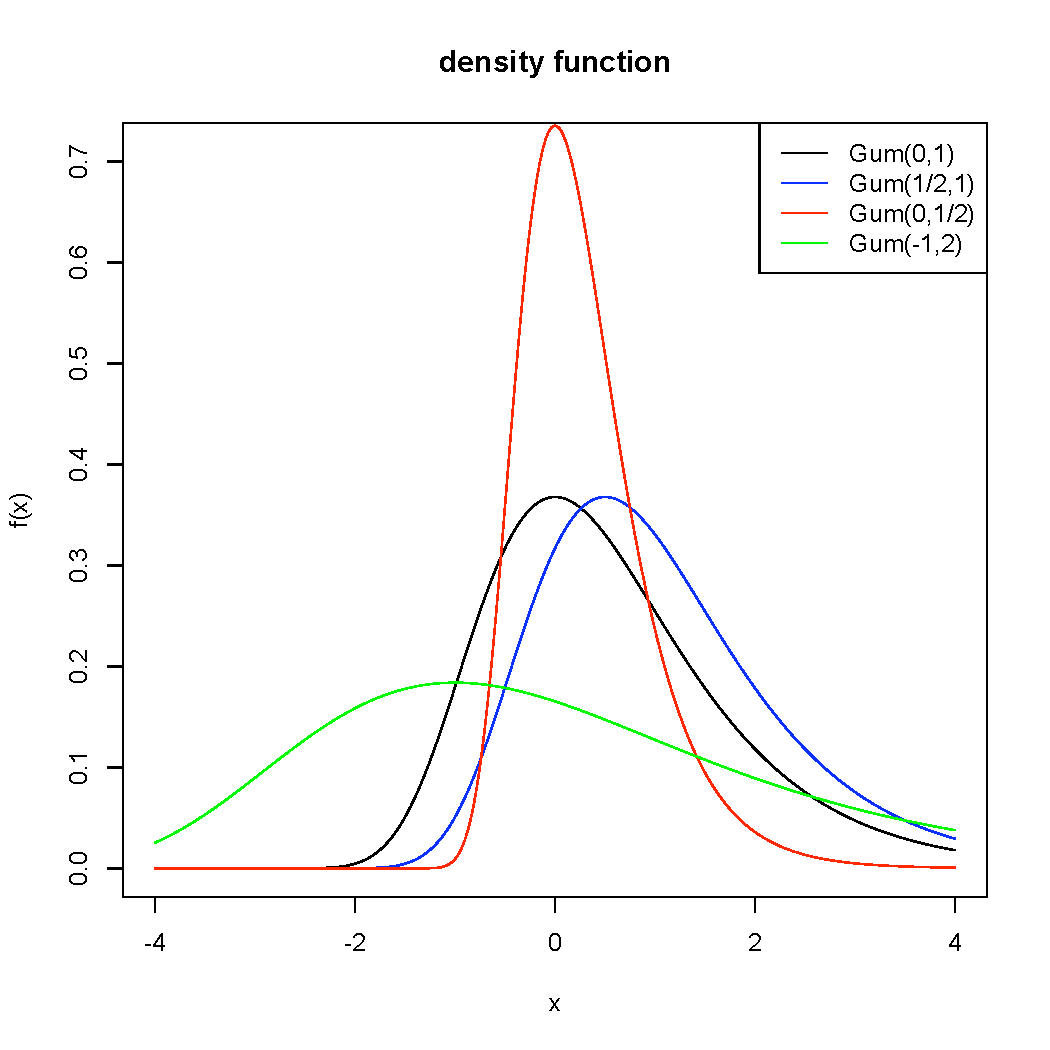
\includegraphics[width=0.48\textwidth]{img/gumbelzoom}
  \end{center}
%  \vspace{-20pt}  
  \caption{Density function for Gumbel distributions}
%  \vspace{-20pt}  
\end{wrapfigure}
The standard Gumbel distribution is defined by the following density function
$$
f(x) = e^{-x-e^{-x}},
$$
where $x\in\mathbb R$. Its distribution function is expressed as follows
$$
F(x) =e^{-e^{-x}}. 
$$

A scaled and shifted version of the Gumbel distribution exists. The density is defined as
$$
f(x)=\frac{1}{\sigma}e^{-\frac{x-\mu}{\sigma}-e^{-\frac{x-\mu}{\sigma}}},
$$
where $x\in\mathbb R$, $\mu\in\mathbb R$ and $\sigma >0$. We get back to the standard Gumbel distribution with $\mu=0$ and $\sigma=1$. The distribution function of the Gumbel I distribution is simply
$$
F(x) = e^{-e^{-\frac{x-\mu}{\sigma}}}, 
$$
for $x\in\mbb R$.

%This is the Gumbel distribution of the first kind. A completely different distribution of the Gumbel distribution can be used
%$$
%f(x) = abx^{a-1}e^{-bx^{-a}},
%$$
%where $x>0$ and $a,b>0$. The distribution function of the Gumbel II is 
%$$
%F(x) =e^{-bx^{-a}}.
%$$

There exists a Gumbel distribution of the second kind defined by the following distribution function
$$
F(x) = 1-e^{-e^{\frac{x-\mu}{\sigma}}},
$$
for $x\in\mbb R$. Hence we have the density
$$
f(x) = \frac{1}{\sigma}e^{\frac{x-\mu}{\sigma}-e^{\frac{x-\mu}{\sigma}}}.
$$
This is the distribution of $-X$ when $X$ is Gumbel I distributed.

The characteristic function of the Gumbel distribution of the first kind exists
$$
\phi(t)=\Gamma(1-i\sigma t)e^{i\mu t},
$$
while its moment generating function are
$$
M(t) = \Gamma(1-\sigma t)e^{\mu t}.
$$

\subsection{Properties}
The expectation of a Gumbel type I distribution is $E(X)=\gamma$, the Euler constant, roughly $0.57721$. Its variance is $Var(X)=\frac{\pi^2}{6}$. Thus for the Fisher-Tippett distribution, we have $E(X)=\mu+\sigma\gamma$ and $Var(X)=\frac{\pi^2\sigma^2}{6}$.

For the Gumbel type II, expectation exists if $a>1$ and variance if $a>2$.

\subsection{Estimation}
Maximum likelihood estimators are solutions of the following system
$$
\left\{
\begin{array}{l}
1=\frac{1}{n}\sum\limits_{i=1}^ne^{-\frac{X_i-\mu}{\sigma}}\\
\frac{1}{n}\sum\limits_{i=1}^n X_i=\frac{1}{n}\sum\limits_{i=1}^nX_i e^{-\frac{X_i-\mu}{\sigma}}
\end{array}
\right.,
$$
which can solved numerically initialized by the moment based estimators
$$
\tilde \mu=\bar X_n-\tilde \sigma\gamma \txtm{and} \tilde \sigma = \sqrt{\frac{6S_n^2}{\pi^2}},
$$
where $\gamma$ is the Euler constant.

\subsection{Random generation}
The quantile function of the Gumbel I distribution is simply $F^{-1}(u)=\mu-\sigma\log(-\log(u))$, thus we can use the inverse function method.

\subsection{Applications}
The Gumbel distribution is widely used in natural catastrophe modelling, especially for maximum flood.
NEED REFERENCE

%%%%%%%%%%%%%%%%%%%%%%%%%%%%%%%%%%%%%%%%%%%%%%%
\section{Fr�chet distribution}
A Fr�chet type distribution is a distribution whose distribution function is 
$$
F(x) = e^{-\left(\frac{x-\mu}{\sigma}\right)^{-\xi}},
$$
for $x\geq \mu$. One can notice this is the inverse Weibull distribution, see section \ref{invweibull} for details.


%%%%%%%%%%%%%%%%%%%%%%%%%%%%%%%%%%%%%%%%%%%%%%%%
\section{Weibull distribution}
A Weibull type distribution is characterized by the following distribution function
$$
F(x) = 1- e^{-\left(\frac{x-\mu}{\sigma}\right)^{\beta}},
$$
for $x\geq \mu$. See section \ref{weibull} for details.



%%%%%%%%%%%%%%%%%%%%%%%%%%%%%%%%%%%%%%%%%%%%%%%%
\section{Generalized extreme value distribution}
\subsection{Characterization}
The generalized extreme value distribution is defined by the following distribution function
$$
F(x)= e^{-\left(1+\xi \frac{x-\mu}{\sigma} \right)^{-\frac{1}{\xi}} },
$$
for $1+\xi\left(\frac{x-\mu}{\sigma}\right)>0$, $\xi$ the shape parameter, $\mu$ the location parameter and 
$\sigma>0$ the scale parameter. We can derive a density function
$$
f(x) =  \frac{1}{\sigma} \left(1+\xi \frac{x-\mu}{\sigma} \right)^{-\frac{1}{\xi}-1}e^{-\left(1+\xi \frac{x-\mu}{\sigma} \right)^{-\frac{1}{\xi}} }.
$$
This distribution is sometimes called the Fisher-Tippett distribution. 

Let us note that the values can be taken in $\mbb R$, $\mbb R_-$ or $\mbb R_+$ according to the sign of $\xi$. The distribution function is generally noted by $H_{\xi,\mu,\sigma}$, wich can expressed with the ``standard'' generalized extreme value distribution $H_{\xi,0,1}$ with a shift and a scaling.
When $\xi$ tends to zero, we get the Gumbel I distribution 
$$
H_{\xi,\mu,\sigma}(x) \underset{\xi\rightarrow 0}{\longrightarrow}  e^{-e^{-\frac{x-\mu}{\sigma}}}.
$$

\subsection{Properties}
The expectation and the variance are
$$
E(X) = \mu-\frac{\sigma}{\xi}\Gamma(1-\xi) \txtm{and} Var(X) = \frac{\sigma^2}{\xi^2}(\Gamma(1-2\xi)-\Gamma^2(1-\xi))
$$
if they exist.

From the extreme value theory, we have the following theorem. Let $(X_i)_{1\leq i\leq n}$ be an i.i.d. sample and $X_{i:n}$ the order statistics. If there exits two sequences $(a_n)_n$ and $(b_n)_n$ valued in 
$\mbb R_+$ and $\mbb R$ respectively, such that 
$$
P\left(\frac{X_{n:n}-b_n}{a_n}\right)
$$
have a limit in probability distribution. Then the limiting distribution $H$ for the maximum belongs to the type of one the following three distribution functions
$$
H(x)=
\left\{
\begin{array}{llr}
e^{-x^{-\xi}}, & x\geq 0, \xi>0, & \txtm{MDA of Fr�chet} \\
e^{-(-x)^{\xi}}, & x\leq 0, \xi<0, & \txtm{MDA of Weibull} \\
e^{-e^{-x}}, & x\in \mbb R, \xi=0, & \txtm{MDA of Gumbel} \\
\end{array}
\right. ,
$$
where MDA stands for maximum domains of attraction. For all distribution, there is a unique MDA. We quickly see that the limiting distribution for the maximum is nothing else than the generalized extreme value distribution $H_{\xi,0,1}$. This theorem is the Fisher-Tippett-Gnedenko theorem. 

For the minimum, assuming that $P\left(\frac{X_{1:n}-b_n}{a_n}\right)$ has a limit, the 
limiting distribution belongs to
$$
\tilde H(x)=
\left\{
\begin{array}{ll}
1-e^{-x^{\beta}}, & x\geq 0, \beta>0  \\
1-e^{-(-x)^{\beta}}, & x\leq 0, \beta<0  \\
1-e^{-e^{x}}, & x\in \mbb R, \beta=0  \\
\end{array}
\right. .
$$

In the MDA of Fr�chet, we have the Cauchy, the Pareto, the Burr, the log-gamma and the stable distributions, while in the Weibull MDA we retrieve the uniform, the beta and bounded support power law distribution. Finally, the MDA of Gumbel contains the exponential, the Weibull, the gamma, the normal, the lognormal, the Benktander distributions. 

From the \cite{tve}, we also have some equivalence given a MDA:
\begin{itemize}
\item a distribution function $F$ belongs to the MDA of Fr�chet if and only if $1- F(x)=x^{-\alpha} L(x)$ for some slowly varying function $L$,
\item a distribution function $F$ belongs to the MDA of Weibull if and only if $1- F(x_F-1/x)=x^{-\alpha} L(x)$ for some slowly varying function $L$ and $x_F<+\infty$,
\item a distribution function $F$ belongs to the MDA of Gumbel if and only if there exists $z<x_F$ such that $1- F(x)=c(x)e^{-\int_z^x\frac{g(t)}{a(t)}dt}$ for some measurable function $c$, $g$ and a continuous function $a$.
\end{itemize}

\subsection{Estimation}
According to \cite{tve} maximum likelihood estimation is not very reliable in the case of the generalized extreme value fitting. But that's not surprising since the generalized extreme value distribution is a limiting distribution to very heterogeneous distribution, such as heavy tailed, light tailed or bounded distributions.

We can use weighted moment method, where we estimate moments
$$
\omega_r(\xi,\mu,\sigma) = E(X H_{\xi,\mu,\sigma}^r(X))
$$
by its empirical equivalent
$$
\hat \omega_r = \frac{1}{n}\sum_{i=1}^n X_{j:n} U_{j:n}^r,
$$
where $U_{j:n}^r$ are the order statistics of an uniform sample (which can be replaced by its expectation $\frac{(n-r-1)!}{(n-1)!} \frac{(n-j)!}{(n-j-r)!} $).
Equalling the theoretical and the empirical moments, we get that $\xi$ is a solution of 
$$
\frac{3\hat \omega_2 -\hat\omega_0}{2\hat\omega_1-\hat\omega_0} = \frac{3^\xi-1}{2^\xi-1}.
$$
Then we estimate the other two parameters with
$$
\hat \sigma = \frac{(2\hat\omega_1-\hat\omega_0)\hat\xi}{\Gamma(1-\hat\xi)(2^{\hat\xi}-1)} \txtm{and}
\hat \mu = \hat\omega_0+\frac{\hat\sigma}{\hat\xi}(1-\Gamma(1-\hat\xi)).
$$


\subsection{Random generation}
The quantile function of the generalized extreme value distribution is 
$F^{-1}(u) = \mu+\frac{\sigma}{\xi}((-\log u)^{-\xi})-1$ for $\xi\neq 0$. So we can use the inverse function method.

\subsection{Applications}
The application of the generalized extreme value distribution is obviously the extremex value theory which can be applied in many fields : natural disaster modelling, insurance/finance extreme risk management,\dots


%%%%%%%%%%%%%%%%%%%%%%%%%%%%%%%%%%%%%%%%%%%%%%%%
\section{Generalized Pareto distribution}
See section \ref{GPD} for details.



\part{Multivariate and generalized distributions}
\chapter{Generalization of common distributions}
%%%%%%%%%%%%%%%%%%%%%%%%%%%%%%%%%%%%%%%%%%%%%%%%%%%
\section{Generalized hyperbolic distribution}
This part entirely comes from \cite{ghyp}.
\subsection{Characterization}
The first way to characterize generalized hyperbolic distributions is to say that the random vector $X$ follows a multivariate $\mathcal G\mathcal H$ distribution if
\begin{equation}\label{eq:ghd}
  X \stackrel{\mathcal{L}}{=} \mu + W \gamma + \sqrt{W} A Z
\end{equation}
where
\begin{enumerate}
\item $Z \sim \mcal N_k(\mathbf{0},I_k)$
\item $A \in \mathbb R^{d \times k}$
\item $ \mu, \gamma \in \mathbb R^{d}$
\item $W \geq 0$ is a scalar-valued random variable which is
  independent of $Z$ and has a Generalized Inverse Gaussian
  distribution, written $GIG(\lambda, \chi, \psi)$.
\end{enumerate}
Note that there are at least five alternative definitions leading to
different parametrizations. 

Nevertheless, the parameters of a $\mathcal G\mathcal H$ distribution given by the above
definition admit the following interpretation:
\begin{itemize}
\item $\lambda, \chi, \psi$ determine the shape of the distribution,
  that is, how much weight is assigned to the tails and to the
  center. In general, the larger those parameters the closer is the
  distribution to the normal distribution.
\item $\mu$ is the location parameter.
\item $\Sigma = A A'$ is the dispersion-matrix.
\item $\gamma$ is the skewness parameter. If $\gamma = 0$, then the
  distribution is symmetric around $\mu$.
\end{itemize}
Observe that the conditional distribution of $X | W = w$ is normal,
\begin{equation}\label{eq:mixture}
  X | W = w \sim\mcal N_d(\mu + w \, \gamma, w \Sigma),
\end{equation}

Another way to define a generalized hyperbolic distribution is to use the density.
Since the conditional distribution of $X$ given $W$ is Gaussian with
mean $\mu + W \gamma$ and variance $ W \Sigma$ the $\mathcal G\mathcal H$ density can be
found by mixing $X | W$ with respect to $W$.
\begin{eqnarray}\label{eq:fghyp}
  f_X(x) &=& \int_0^\infty f_{X|W}(x|w) \, f_W(w) \, dw \\ \nonumber
  &=& \int_0^\infty
  \frac{e^{(x-\mu)' \Sigma^{-1} \gamma}}
  {(2\pi)^{\frac{d}{2}} \left|\Sigma\right|^{\frac{1}{2}}w^{\frac{d}{2}}}
  \exp\left\{ -\frac{Q(x)}{2w}-\frac{\gamma \Sigma \gamma}{2/w} \right\}
  f_W(w)dw \\ \nonumber
  &=& \frac{(\sqrt{\psi/\chi})^\lambda
    (\psi + \gamma \Sigma \gamma)^{\frac{d}{2}-\lambda}}
  {(2\pi)^{\frac{d}{2}} \left|\Sigma\right| ^\frac{1}{2}
    K_\lambda(\sqrt{\chi\psi})}\times
  \frac{K_{\lambda - \frac{d}{2}}(
    \sqrt{(\chi + Q(x))(\psi + \gamma \Sigma \gamma)})\;
    e^{(x - \mu)'\Sigma^{-1} \gamma}}
  {(\sqrt{(\chi + Q(x))(\psi + \gamma \Sigma \gamma)})^{\frac{d}{2} - \lambda}},
\end{eqnarray}
where $K_\lambda(\cdot)$ denotes the modified Bessel
function of the third kind and $Q(x)$ denotes the mahalanobis distance $Q(x) =
(x - \mu)' \Sigma^{-1} (x - \mu)$ (i.e. the distance with $\Sigma^{-1}$ as norm).  
The domain of variation of the
parameters $\lambda, \chi$ and $\psi$ is given in section
\ref{sec:param}.

A last way to characterize generalized hyperbolic distributions is the usage of moment generating functions. An appealing property of normal mixtures is that the moment generating
function is easily calculated once the moment generating function of
the mixture is known. Based on equation (\ref{eq:moment-gen-gig}) we
obtain the moment generating function of a $\mathcal G\mathcal H$ distributed random
variable $X$ as
\begin{eqnarray}
\label{eq:moment-gen-gig}
    M(t) &=& E(E(\exp \left\{t' X\right\} | W)) =
    e^{t'\mu} E(\exp \left\{W \left(t' \gamma + 1/2~t'
          \Sigma t\right) \right\}  ) \nonumber \\
    &=& e^{t' \mu} \left(\frac{\psi}{\psi - 2 t'
        \gamma - t' \Sigma t}\right)^{\lambda / 2}
    \frac{K_\lambda(\sqrt{\psi (\chi - 2 t'
        \gamma - t' \Sigma t)})}{K_\lambda(\sqrt{\chi
        \psi})}, \quad \chi \geq 2~t' \gamma + t' \Sigma
    t. \nonumber
\end{eqnarray}
For moment generating functions of the special cases of the $\mathcal G\mathcal H$
distribution we refer to \cite{Prause1999} and \cite{Paolella2007}.

\subsection{Parametrization}\label{sec:param}
% <---------------------------------------------------------------------->
There are several alternative parametrizations for the GH
distribution.  In the~\soft{R}~package~\soft{ghyp}~the user can choose between
three of them.  There exist further parametrizations which are not
implemented and not mentioned here. For these parametrizations we
refer to \cite{Prause1999} and \cite{Paolella2007}.

Table \ref{tab:param} describes the parameter ranges for each
parametrization and each special case. Clearly, the dispersion
matrices $\Sigma$ and $\Delta$ have to fulfill the usual conditions
for covariance matrices, i.e., symmetry and positive definiteness as
well as full rank.

\begin{table}[h]
  \begin{small}
    \begin{tabular}{l | c c c c c c}
      & \multicolumn{6}{c}{$(\lambda,\chi,\psi,\mu,\Sigma,\gamma)$-Parametrization} \\
      &  $\lambda$ & $\chi$ & $\psi$ & $\mu$ & $\Sigma$ & $\gamma$\\
      \hline
      ghyp & $\lambda \in\mbb R$ & $\chi > 0$ & $\psi > 0$ & $\mu \in\mbb R^d$ & $\Sigma \in\mbb R^\Sigma$ & $\gamma \in\mbb R^d$\\
      hyp & $\lambda = \frac{d + 1}{2} $ & $\chi > 0$ & $\psi > 0$ & $\mu \in\mbb R^d$ & $\Sigma \in\mbb R^\Sigma$ & $\gamma \in\mbb R^d$\\
      NIG & $\lambda = - \frac{1}{2}$ & $\chi > 0$ & $\psi > 0$ & $\mu \in\mbb R^d$ & $\Sigma \in\mbb R^\Sigma$ & $\gamma \in\mbb R^d$\\
      t & $\lambda < 0$ & $\chi > 0$ & $\psi = 0$ & $\mu \in\mbb R^d$ & $\Sigma \in\mbb R^\Sigma$ & $\gamma \in\mbb R^d$\\
      VG & $\lambda > 0$ & $\chi = 0$ & $\psi > 0$ & $\mu \in\mbb R^d$ & $\Sigma \in\mbb R^\Sigma$ & $\gamma \in\mbb R^d$\\
      \hline
      \\
      % -------------------------------------------------------------------------
      & \multicolumn{6}{c}{$(\lambda,\bar\alpha,\mu,\Sigma,\gamma)$-Parametrization} \\
      &  $\lambda$ & $\bar\alpha$ & $\mu$ & $\Sigma$ & $\gamma$\\
      \hline
      ghyp & $\lambda \in\mbb R$ & $\bar\alpha > 0$ & $\mu \in\mbb R^d$ & $\Sigma \in\mbb R^\Sigma$ & $\gamma \in\mbb R^d$\\
      hyp & $\lambda = \frac{d + 1}{2} $ & $\bar\alpha > 0$  & $\mu \in\mbb R^d$ & $\Sigma \in\mbb R^\Sigma$ & $\gamma \in\mbb R^d$\\
      NIG & $\lambda = \frac{1}{2}$ & $\bar\alpha > 0$ &  $\mu \in\mbb R^d$ & $\Sigma \in\mbb R^\Sigma$ & $\gamma \in\mbb R^d$\\
      t & $\lambda = - \frac{\nu}{2} < -1$ & $\bar\alpha = 0$ &   $\mu \in\mbb R^d$ & $\Sigma \in\mbb R^\Sigma$ & $\gamma \in\mbb R^d$\\
      VG & $\lambda > 0$ & $\bar\alpha = 0$ &  $\mu \in\mbb R^d$ & $\Sigma \in\mbb R^\Sigma$ & $\gamma \in\mbb R^d$\\
      \hline
      \\
      % -------------------------------------------------------------------------
      & \multicolumn{6}{c}{$(\lambda,\alpha,\mu,\Sigma,\delta,\beta)$-Parametrization} \\
      &  $\lambda$ & $\alpha$ & $\delta$ & $\mu$ & $\Delta$ & $\beta$\\
      \hline
      ghyp & $\lambda \in\mbb R$ & $\alpha > 0$ & $\delta > 0$ & $\mu \in\mbb R^d$ & $\Delta \in\mbb R^\Delta$ & $\beta \in \{x \in\mbb R^d : \alpha^2 - x' \Delta x > 0\}$ \\
      hyp & $\lambda = \frac{d + 1}{2} $ & $\alpha > 0$ & $\delta > 0$ & $\mu \in\mbb R^d$ & $\Delta \in\mbb R^\Delta$  & $\beta \in \{x \in\mbb R^d : \alpha^2 - x' \Delta x > 0\}$ \\
      NIG & $\lambda = - \frac{1}{2}$ & $\alpha > 0$ & $\delta > 0$ & $\mu \in\mbb R^d$ & $\Delta \in\mbb R^\Delta$  & $\beta \in \{x \in\mbb R^d : \alpha^2 - x' \Delta x > 0\}$\\
      t & $\lambda < 0$ & $\alpha = \sqrt{\beta' \Delta \beta}$ & $\delta > 0$ & $\mu \in\mbb R^d$ & $\Delta \in\mbb R^\Delta$  & $\beta \in\mbb R^d$ \\
      VG & $\lambda > 0$ & $\alpha > 0$ & $\delta = 0$ & $\mu \in\mbb R^d$ & $\Delta \in\mbb R^\Delta$  & $\beta \in \{x \in\mbb R^d : \alpha^2 - x' \Delta x > 0\}$\\
      \hline
    \end{tabular}
  \end{small}
  \caption{The domain of variation for the parameters of the GH distribution and
    some of its special cases for different parametrizations. We denote the set of all feasible covariance
    matrices in $\mbb R^{d \times d}$ with $\mbb R^\Sigma$.
    Furthermore, let $\mbb R^\Delta = \{A \in\mbb R^\Sigma : |A| = 1\}$.}\label{tab:param}
\end{table}

Internally, he package \soft{ghyp}~uses the
$(\lambda,\chi,\psi,\mu,\Sigma,\gamma)$-parametrization. However, fitting is done in the
($\lambda,\bar\alpha,\mu,\Sigma,\gamma$)-parametrization since this parametrization does not
necessitate additional constraints to eliminate the redundant degree
of freedom.  Consequently, what cannot be represented by the
($\lambda,\alpha,\mu,\Sigma,\delta,\beta$)-parametrization cannot be fitted (cf. section
\ref{sec:lambdaabarparam}).
% <---------------------------------------------------------------------->
\subsubsection{$(\lambda,\chi,\psi,\mu,\Sigma,\gamma)$-Parametrization}\label{sec:chi-psi-param}
% <---------------------------------------------------------------------->
The ($\lambda,\chi,\psi,\mu,\Sigma,\gamma$)-parametrization is obtained as the normal
mean-variance mixture distribution when $W \sim GIG(\lambda, \chi,
\psi)$.  This parametrization has a drawback of an identification
problem. Indeed, the distributions $GH_d(\lambda,\chi,\psi,\mu,\Sigma,\gamma)$ and 
$GH_d(\lambda,\chi/k,k\psi,\mu,k\Sigma,k\gamma)$ are identical for
any $k > 0$. Therefore, an identifying problem occurs when we start to
fit the parameters of a GH distribution to data. This problem could be
solved by introducing a suitable contraint. One possibility is to
require the determinant of the dispersion matrix $\Sigma$ to be $1$.
% <---------------------------------------------------------------------->
\subsubsection{($\lambda,\bar\alpha,\mu,\Sigma,\gamma$)-Parametrization}\label{sec:lambdaabarparam}
% <---------------------------------------------------------------------->
There is a more elegant way to eliminate the degree of freedom. We
simply constrain the expected value of the generalized inverse
Gaussian distributed mixing variable $W$ to be $1$
(cf. \ref{sec:gig}). This makes the interpretation of the skewness
parameters $\gamma$
easier and in addition, the fitting procedure becomes faster (cf. \ref{sec:EM}). \\
We define
\begin{equation}
  E(W)  =  \sqrt{\frac{\chi}{\psi}}\frac{K_{\lambda+1}(\sqrt{\chi\psi})}
  {K_{\lambda}{(\sqrt{\chi\psi})}} = 1.
\end{equation}
and set
\begin{equation}
  \bar\alpha = \sqrt{\chi\psi}.
\end{equation}
It follows that
\begin{equation} \label{eq:abartochipsi} \psi = \bar\alpha \;
  \frac{K_{\lambda+1}(\bar\alpha)}{K_{\lambda} (\bar\alpha)} \;
  \hbox{and} \; \chi = \frac{\bar\alpha^2}{\psi}= \bar\alpha \;
  \frac{K_{\lambda}(\bar\alpha)}{K_{\lambda+1} (\bar\alpha)}.
\end{equation}
The drawback of the ($\lambda,\bar\alpha,\mu,\Sigma,\gamma$)-parametrization is that it does
not exist in the case $\bar\alpha = 0$ and $\lambda \in [-1,0]$, which
corresponds to a Student-t distribution with non-existing
variance. Note that the ($\lambda,\bar\alpha,\mu,\Sigma,\gamma$)-parametrization yields to a
slightly different parametrization for the special case of a Student-t
distribution.
% <---------------------------------------------------------------------->
\subsubsection{$(\lambda,\alpha,\mu,\Sigma,\delta,\beta)$-Parametrization}
% <---------------------------------------------------------------------->
When the GH distribution was introduced in \citet{Barndorffnielsen77},
the following parametrization for the multivariate case was used.
\begin{equation}
  f_X(x)  = \frac{ (\alpha^2-\beta'\Delta\beta)^{\lambda /2}}{(2\pi)^{\frac{d}{2}} \sqrt{|\Delta|} \, \delta^\lambda \,
    K_{\lambda}(\delta \sqrt{\alpha^2-\beta'\Delta\beta})}\times
  \frac{K_{\lambda - \frac{d}{2}}(\alpha \sqrt{\delta^2 + (x-\mu)'\Delta^{-1}(x-\mu)}) \;
    e^{\beta' (x - \mu)}}{(\alpha \sqrt{\delta^2 + (x-\mu)'\Delta^{-1}(x-\mu)})^{\frac{d}{2} - \lambda}},
\end{equation}
where the determinant of $\Delta$ is constrained to be $1$.  In the
univariate case the above expression reduces to
\begin{equation}
  f_X(x)  = \frac{ (\alpha^2 - \beta^2)^{\lambda /2}}
  {\sqrt{2\pi} \, \alpha^{\lambda - \frac{1}{2}} \, \delta^\lambda \,
    K_{\lambda}(\delta \sqrt{\alpha^2 - \beta^2})}\times
  K_{\lambda - \frac{1}{2}}(\alpha \sqrt{\delta^2 + (x - \mu)^2}) \;
  e^{\beta (x - \mu)},
\end{equation}
which is the most widely used parametrization of the GH distribution
in literature.
% <---------------------------------------------------------------------->
\subsubsection{Switching between different parametrizations}
% <---------------------------------------------------------------------->
The following formulas can be used to switch between the
($\lambda,\bar\alpha,\mu,\Sigma,\gamma$), ($\lambda,\chi,\psi,\mu,\Sigma,\gamma$), and the
($\lambda,\alpha,\mu,\Sigma,\delta,\beta$)-parametrization. The parameters $\lambda$
and $\mu$ remain the same, regardless of the parametrization. \\
The way to obtain the ($\lambda,\alpha,\mu,\Sigma,\delta,\beta$)-parametrization from the
($\lambda,\bar\alpha,\mu,\Sigma,\gamma$)-parametrization yields over the
($\lambda,\chi,\psi,\mu,\Sigma,\gamma$)-parametrization:
$$(\lambda,\bar\alpha,\mu,\Sigma,\gamma) \quad \leftrightarrows \quad (\lambda,\chi,\psi,\mu,\Sigma,\gamma)
\quad \leftrightarrows \quad (\lambda,\alpha,\mu,\Sigma,\delta,\beta)$$
\begin{description}
\item[$(\lambda,\bar\alpha,\mu,\Sigma,\gamma) \rightarrow (\lambda,\chi,\psi,\mu,\Sigma,\gamma)$:] Use the relations
  in (\ref{eq:abartochipsi}) to obtain $\chi$ and $\psi$.  The
  parameters $\Sigma$ and $\gamma$ remain the same.
\item[$(\lambda,\chi,\psi,\mu,\Sigma,\gamma) \rightarrow (\lambda,\bar\alpha,\mu,\Sigma,\gamma)$:] Set $k =
  \sqrt{\frac{\chi}{\psi}}\frac{K_{\lambda+1}(\sqrt{\chi\psi})}
  {K_{\lambda}{(\sqrt{\chi\psi})}}.$
  \begin{equation}
    \bar\alpha = \sqrt{\chi\psi} , \quad \Sigma \equiv k \, \Sigma, \quad \gamma \equiv k \, \gamma
  \end{equation}
\item[$(\lambda,\chi,\psi,\mu,\Sigma,\gamma) \rightarrow (\lambda,\alpha,\mu,\Sigma,\delta,\beta)$:]
  \begin{eqnarray}
    \Delta = |\Sigma|^{-\frac{1}{d}} \Sigma &,& \beta = \Sigma^{-1} \gamma \nonumber \\
    \delta = \sqrt{\chi |\Sigma|^{\frac{1}{d}}} &,& \alpha =
    \sqrt{|\Sigma|^{-\frac{1}{d}} (\psi + \gamma'\Sigma^{-1}\gamma)}
  \end{eqnarray}
\item[$(\lambda,\alpha,\mu,\Sigma,\delta,\beta) \rightarrow (\lambda,\chi,\psi,\mu,\Sigma,\gamma)$:]
  \begin{equation}
    \Sigma = \Delta , \quad \gamma = \Delta \beta , \quad \chi =
    \delta^2 ,
    \quad \psi = \alpha^2 - \beta' \Delta \beta .
  \end{equation}
\end{description}
%---------------------------%---------------------------%---------------------------%---------------------------

\subsection{Properties}
\subsubsection{Moments}
The expected value and the variance are given by
\begin{eqnarray}
\label{eq:momentgig}
  E(X)  &=& \mu + E(W) \gamma \\
  Var(X)  &=& E(Cov(X | W)) + Cov(E(X| X)) \\ \nonumber
  &=& Var(W) \gamma \gamma'  + E(W) \Sigma.
\end{eqnarray}

\subsubsection{Linear transformation}
The GH class is closed under linear transformations:
%\begin{proposition}
  If $X \sim GH_d(\lambda,\chi,\psi,\mu,\Sigma,\gamma)$ and $Y = B X + \mathbf{b}$, where $B \in
  \mbb R^{k \times d}$ and $\mathbf{b} \in \mbb R^k$, then $Y
  \sim GH_k(\lambda,\chi,\psi,B\mu+\mathbf{b},B\Sigma B',B\gamma)$.
%\end{proposition}
%\begin{proof}
%  The characteristic function of $X$ is
%  $$\phi_X(\tvec) = E\left(E\left(e^{i \, \tvec' X\right) | W\right) =
%  E\left(e^{i \, \tvec' (\mu + W \gamma) - 1/2 \, W \, \tvec' \, \Sigma
%      \, \tvec}\right) = e^{i \, \tvec' \mu} \, \hat{H}(1/2 \, \tvec' \,
%  \Sigma \, \tvec - i \, \tvec' \gamma),$$ where $\hat{H}(\theta) =
%  \int_0^\infty e^{-\theta v} dH(v)$ denotes the Laplace-Stieltjes
%  transform of the distribution function $H$ of $W$. Let $\Y = B \, X
%  + \mathbf{b}$. The characteristic function is then
%  \begin{eqnarray*}
%    \phi_Y(t) &=& E\left(E\left(e^{i \, \tvec' \, (B \, X  + \mathbf{b})} | W\right)\right) =
%    E\left(e^{i \, \tvec' \, (B (\mu + W \gamma) + \mathbf{b}) -
%        1/2 \, W \,\tvec' \, B \, \Sigma \, B' \, \tvec}\right)\\
%    &=& e^{i \, \tvec' \, (B \, \mu + \mathbf{b})} \, \hat{H}(1/2 \, W
%    \, \tvec' \, B \, \Sigma \, B' \, \tvec -  i \, \tvec' B \, \gamma).
%  \end{eqnarray*}
%  Therefore, $B X + \mathbf{b} \sim \GHtransf$.
%\end{proof}
Observe that by introducing a new skewness parameter $\bar{\gamma} =
\Sigma \gamma$, all the shape and skewness parameters ($\lambda, \chi,
\psi, \bar{\gamma}$) become location and scale-invariant, provided the
transformation does not affect the dimensionality, that is
$B \in\mbb R^{d \times d}$ and $\mathbf{b} \in\mbb R^d$.


\subsection{Special cases}\label{sec:specialcases}
% <---------------------------------------------------------------------->
The GH distribution contains several special cases known under special
names.
\begin{itemize}
\item{If $\lambda = \frac{d+1}{2}$ the name generalized is dropped and
    we have a multivariate \emph{hyperbolic (hyp)} distribution. The
    univariate margins are still GH distributed. Inversely, when
    $\lambda = 1$ we get a multivariate GH distribution with
    hyperbolic margins.}
\item{If $\lambda = -\frac{1}{2}$ the distribution is called
    \emph{Normal Inverse Gaussian (NIG)}.}
\item{If $\chi = 0$ and $\lambda > 0$ one gets a limiting case which
    is known amongst others as \emph{Variance Gamma (VG)}
    distribution.}
\item{If $\psi = 0$ and $\lambda < -1$ one gets a limiting case which
    is known as a \emph{generalized hyperbolic Student-t} distribution
    (called simply \emph{Student-t} in what follows).}
\end{itemize}
%Further information about the special cases and the necessary formulas
%to fit these distributions to multivariate data can be found in the
%appendixes \ref{sec:gig} and \ref{sec:dens_special_cases}. The
%parameter constraints for the special cases in different
%parametrizations are described in the following section.

\subsection{Estimation}
% <---------------------------------------------------------------------->
%\section{Fitting generalized hyperbolic distributions to data}
% <---------------------------------------------------------------------->
Numerical optimizers can be used to fit univariate GH
distributions to data by means of maximum likelihood estimation.
Multivariate GH distributions
can be fitted with expectation-maximazion (EM) type algorithms (see
\citet{Dempster.1977} and \citet{Meng.1993}).
%-------------------------------------------------------------------------
\subsubsection{EM-Scheme}\label{sec:EM}
% <---------------------------------------------------------------------->
Assume we have iid data $x_1,\ldots,x_n$ and parameters represented
by $\Theta = (\lambda,\bar\alpha,\mu,\Sigma,\gamma)$. The problem is to maximize
\begin{equation}
  \ln L(\Theta;x_1,\ldots,x_n) = \sum_{i=1}^n \ln f_X(x_i;\Theta).
\end{equation}
This problem is not easy to solve due to the number of parameters and
necessity of maximizing over covariance matrices.  We can proceed by
introducing an augmented likelihood function
\begin{equation}\label{eq:likelihood}
  \ln \tilde{L}(\Theta;x_1,\ldots,x_n,w_1,\ldots,w_n) =
  \sum_{i=1}^n \ln f_{X|W}(x_i|w_i;\mu,\Sigma,\gamma) +
  \sum_{i=1}^n \ln f_W(w_i;\lambda,\bar\alpha)
\end{equation}
and spend the effort on the estimation of the latent mixing variables
$w_i$ coming from the mixture representation (\ref{eq:mixture}).  This
is where the EM algorithm comes into play.
\begin{description}
\item[\textbf{E-step:}]{Calculate the conditional expectation of the
    likelihood function (\ref{eq:likelihood}) given the data
    $x_1,\ldots,x_n$ and the current estimates of parameters
    $\Theta^{[k]}$}.  This results in the objective function
  \begin{equation}
    Q(\Theta;\Theta^{[k]})=E\left(
      \ln \tilde{L}(\Theta;x_1,\ldots,x_n,w_1,\ldots,w_n)|
      x_1,\ldots,x_n;\Theta^{[k]}\right).
  \end{equation}

\item[\textbf{M-step:}]{Maximize the objective function with respect
    to $\Theta$ to obtain the next set of estimates $\Theta^{[k+1]}$.}
\end{description}
Alternating between these steps yields to the maximum likelihood
estimation of the parameter set $\Theta$. In practice,
performing the E-Step means maximizing the second summand of
(\ref{eq:likelihood}) numerically. The log density of the GIG
distribution (cf. \ref{eq:densgig}) is
\begin{equation}\label{eq:logfgig}
  \ln f_W(w) = \frac{\lambda}{2} \ln(\psi/\chi) - \ln(2 K_\lambda(\sqrt{\chi\psi}) )
  + (\lambda - 1) \ln w -\frac{\chi}{2} \frac{1}{w} - \frac{\psi}{2} w.
\end{equation}
When using the ($\lambda,\bar\alpha$)-parametrization this problem is of
dimension two instead of three as it is in the ($\lambda, \chi,
\psi$)-parametrization.
As a consequence the performance increases.\\
Since the $w_i$'s are latent one has to replace $w$, $1/w$ and $\ln w$
with the respective expected values in order to maximize the log
likelihood function.  Let
\begin{equation} \label{eq:etadeltaxi} \eta_i^{[k]} := E\left(w_i \, | \,
    x_i;\Theta^{[k]}\right),\; \delta_i^{[k]} := E\left(w_i^{-1} \, | \,
    x_i;\Theta^{[k]}\right),\; xi_i^{[k]} := E\left(\ln w_i \, | \, x_i;\Theta^{[k]}\right).
\end{equation}
We have to find the conditional density of $w_i$ given $x_i$ to
calculate these quantities.
% <---------------------------------------------------------------------->
\subsubsection{MCECM estimation}
% <---------------------------------------------------------------------->
In the \texttt{R} implementation a modified EM scheme is used, which
is called multi-cycle, expectation, conditional estimation (MCECM)
algorithm \citep*{Meng.1993, QRMmcneil05}.  The different steps of the
MCECM algorithm are sketched as follows:
\renewcommand{\labelenumi}{(\arabic{enumi})}
\begin{enumerate}
\item{Select reasonable starting values for $\Theta^{[k]}$.  For example
    $\lambda = 1$, $\bar\alpha= 1$, $\mu$ is set to the sample mean,
    $\Sigma$ to the sample covariance matrix and $\gamma$ to a zero
    skewness vector.  }
\item{Calculate $\chi^{[k]}$ and $\psi^{[k]}$ as a function of
    $\bar\alpha^{[k]}$ using (\ref{eq:abartochipsi}).  }
\item{Use (\ref{eq:etadeltaxi}), (\ref{eq:momentgig}) to calculate the weights $\eta_i^{[k]}$ and
    $\delta_i^{[k]}$. Average the weights to get
    \begin{equation}
      \bar{\eta}^{[k]} = \frac{1}{n} \sum_{i=1}^{n} \eta_i^{[k]}
      \; \hbox{and} \;
      \bar{\delta}^{[k]} = \frac{1}{n} \sum_{i=1}^{n} \delta_i^{[k]}.
    \end{equation}
  }
\item{If an asymmetric model is to be fitted set $\gamma$ to
    $\mathbf{0}$, else set
    \begin{equation}
      \gamma^{[k+1]}= \frac{1}{n} \frac{\sum_{i=1}^{n} \delta_i^{[k]} (\bar{x}-x_i)}
      {\bar{\eta}^{[k]} \bar{\delta}^{[k]} - 1}.
    \end{equation}
  }
\item{Update $\mu$ and $\Sigma$:
    \begin{eqnarray}
      \mu^{[k+1]} &=& \frac{1}{n} \frac{\sum_{i=1}^{n} \delta_i^{[k]} (x_i-\gamma^{[k+1]})}
      {\bar{\delta}^{[k]}}\\
      \Sigma^{[k+1]} &=& \frac{1}{n} \sum_{i=1}^{n} \delta_i^{[k]} (x_i-\mu^{[k+1]})(x_i-\mu^{[k+1]})'
      - \bar{\eta}^{[k]} \gamma^{[k+1]} \gamma^{[k+1]}\,'.
    \end{eqnarray}
  }
\item{Set $\Theta^{[k,2]} = (\lambda^{[k]}, \bar\alpha^{[k]},\mu^{[k+1]},
    \Sigma^{[k+1]}, \gamma^{[k+1]})$ and calculate weights
    $\eta_i^{[k,2]}$, $\delta_i^{[k,2]}$ and $xi_i^{[k,2]}$ using
    (\ref{eq:etadeltaxi}), (\ref{eq:eloggig}) and
    (\ref{eq:momentgig}).  }
\item{Maximize the second summand of (\ref{eq:likelihood}) with
    density (\ref{eq:logfgig}) with respect to $\lambda$, $\chi$ and
    $\psi$ to complete the calculation of $\Theta^{[k,2]}$ and go back
    to step (2). Note that the objective function must calculate
    $\chi$ and $\psi$ in dependence of $\lambda$ and $\bar\alpha$ using
    relation (\ref{eq:abartochipsi}).  }
\end{enumerate}
% <---------------------------------------------------------------------->



\subsection{Random generation}
We can simply use the first characterization by adding
$$
 \mu + W \gamma + \sqrt{W} A Z
$$
where $Z$ is a multivariate gaussian vector $\mcal N_k(\mathbf{0},I_k)$ and $W$ follows a 
Generalized Inverse Gaussian $GIG(\lambda, \chi, \psi)$.


\subsection{Applications}
NEED REFENCE

%%%%%%%%%%%%%%%%%%%%%%%%%%%%%%%%%%%%%%%%%%%%%%%%%%%
\section{Stable distribution}
A detailed and complete review of stable distributions can be found in \cite{nolan:2009}.
\subsection{Characterization}
Stable distributions are characterized by the following equation
$$
a\tilde X+b\underset{\tilde{}}{X} \stackrel{\mcal L}{=} cX+d,
$$
where $\tilde X$ and $\underset{\tilde{}}{X}$ are independent copies of a random variable $X$ and some positive constants $a, b, c$ and $d$. This equation means stable distributions are distributions closed for linear combinations. For the terminology, we say $X$ is strictly stable if $d=0$ and symmetric stable if in addition we have $X\stackrel{\mcal L}{=} -X$.
From \cite{nolan:2009}, we learn we use the word stable since the shape of the distribution is preserved under linear combinations.

Another way to define stable distribution is to use characteristic functions. $X$ has a stable distribution if and only if 
its characteristic function is
$$
\phi(t) = e^{it \delta}\times\left\{
\begin{array}{ll}
e^{-|t \gamma |^\alpha(1-i\beta\tan(\frac{\pi\alpha}{2})\sign(t))} & \txtm{if}\alpha\neq 1\\
e^{-|t \gamma |(1+i\beta\frac{2}{\pi}\log|t |\sign(t))} & \txtm{if}\alpha= 1\\
\end{array}
\right. ,
$$
where $\alpha\in]0,2]$, $\beta\in]-1,1[$, $\gamma>0$ and $b\in\mbb R$ are the parameters. In the following, we denote $\mcal S(\alpha,\beta, \gamma,\delta)$, where
$\delta $ is a location parameter, $\gamma$ a scale parameter, $\alpha$ an index of stability and $\beta$ a skewness parameter. This corresponds to the parametrization 1 of \cite{nolan:2009}.

We know that stable distributions $\mcal S(\alpha,\beta, \gamma,\delta)$ are continuous distributions whose support is 
$$
\left\{
\begin{array}{cl}
[\delta,+\infty[ & \txtm{if} \alpha<1 \txtm{and} \beta=1\\
]-\infty, \delta] & \txtm{if} \alpha<1 \txtm{and} \beta=-1\\
]-\infty, +\infty[ & \txtm{otherwise}
\end{array}
\right. .
$$

\subsection{Properties}
If we work with standard stable distributions $\mcal S(\alpha,\beta, 0,1)$, we have the reflection property. That is to say if $X\sim \mcal S(\alpha,\beta, 0,1)$, then $-X\sim \mcal S(\alpha,-\beta, 0,1)$. This implies the following constraint on the density and the distribution function:
$$
f_X(x) = f_{-X}(-x) \txtm{and}
F_X(x) = 1-F_{-X}(x).$$

From the definition, we have the obvious property on the sum. If $X$ follows a stable distribution $\mcal S(\alpha,\beta, \gamma,\delta)$, then $aX+b$ follows a stable distribution of parameters
$$
\left\{
\begin{array}{cl}
\mcal S(\alpha,\sign(a)\beta, |a|\gamma,a\delta+b) & \txtm{if} \alpha\neq 1\\
\mcal S(1,\sign(a)\beta, |a|\gamma,a\delta+b-\frac{2}{\pi}\beta\gamma a\log|a|) & \txtm{if} \alpha= 1
\end{array}
\right. .
$$ 

Furthermore if $X_1$ and $X_2$ follow a stable distribution $\mcal S(\alpha,\beta_i, \gamma_i,\delta_i)$ for $i=1,2$, then 
the sum $X_1+X_2$ follows a stable distribution $\mcal S(\alpha,\beta, \gamma,\delta)$ with $\beta=\frac{\beta_1\gamma_1^\alpha+\beta_2\gamma_2^\alpha}{\gamma_1^\alpha+\gamma_2^\alpha}$, $\gamma=(\gamma_1^\alpha+\gamma_2^\alpha)^{\frac{1}{\alpha}}$ and
$\delta=\delta_1+\delta_2$.

\subsection{Special cases}
The following distributions are special cases of stable distributions:
\begin{itemize}
\item $\mcal S(2,0,\sigma/\sqrt 2,\mu)$ is a Normal distribution defined by the density $f(x) = \frac{1}{\sqrt{2\pi \sigma^2}} e^{-\frac{(x-\mu)^2}{2\sigma^2}}$,
\item $\mcal S(1,0,\gamma,\delta)$ is a Cauchy distribution defined by the density $f(x) = \frac{1}{\pi}\frac{\gamma}{\gamma^2+(x-\gamma)^2}$,
\item $\mcal S(1/2,1,\gamma,\delta)$ is a L�vy distribution defined by the density $f(x) = \sqrt{\frac{\gamma}{2\pi}} \frac{1}{(x-\delta)^{\frac{3}{2}}} e^{-\frac{\gamma}{2(x-\delta)}}$.
\end{itemize}

\subsection{Estimation}
NEED REFERENCE
\subsection{Random generation}
Simulation of stable distributions are carried out by the following algorithm from \cite{chambers}.
Let $\Theta$ be an independent random uniform variable $\mcal U(-\pi/2,\pi/2)$ and $W$ be an exponential variable with mean 1 independent from $\Theta$. For $0<\alpha\leq 2$, we have 
\begin{itemize}
\item in the symmetric case, 
$$
Z = \frac{\sin(\alpha\Theta)}{\cos(\Theta)^{\frac{1}{\alpha}}} \left(\frac{\cos((\alpha-1)\Theta)}{W} \right)^{\frac{1-\alpha}{\alpha}}
$$ follows a stable distribution $\mcal S(\alpha,0, 1,0)$ with the limiting case $\tan(\Theta)$ when $\alpha\rightarrow 1$.
\item in the nonsymetric case,
$$
Z = \left\{
\begin{array}{ll}
\frac{\sin(\alpha(\Theta+\theta))}{(\cos(\alpha\theta)\cos(\Theta))^{\frac{1}{\alpha}}} \left(\frac{\cos(\alpha\theta+(\alpha-1)\Theta)}{W} \right)^{\frac{1-\alpha}{\alpha}}\\
\frac{2}{\pi} \left((\frac{\pi}{2}+\beta\Theta)\tan(\Theta)-\beta\log\left(\frac{\frac{\pi}{2}W\cos(\Theta)}{\frac{\pi}{2}+\beta\Theta}\right)\right)
\end{array}
\right.
$$
follows a stable distribution $\mcal S(\alpha,\beta, 1,0)$ where $\theta=\arctan(\beta\tan(\pi\alpha/2))/\alpha$.
\end{itemize}
Then we get a ``full'' stable distribution with $\gamma Z+\delta$.


\subsection{Applications}
NEED REFERENCE

%%%%%%%%%%%%%%%%%%%%%%%%%%%%%%%%%%%%%%%%%%%%%%%%%%%
\section{Phase-type distribution}
\subsection{Characterization}
A phase-type distribution $PH(\pi,T,m)$ ($\pi$ a row vector of $\mathbb R^m$, $T$ a $m\times m$ matrix) 
is defined as the distribution of the time to absorption in the state $0$
of a Markov jump process, on the set $\{ 0,1,\dots,m\}$, with initial probability $(0,\pi)$ and intensity
matrix\footnote{matrix such that its row sums are equal to $0$ and have positive elements except on its diagonal.} 
$$
\Lambda= (\lambda_{ij})_{ij} = 
\left(
\begin{array}{c|c}
0 & 0\\
\hline
t_0 & T
\end{array}
\right),
$$
where the vector $t_0$ is $-T \mathbf{1}_m$ and $\mathbf{1}_m$ stands for the column vector of $1$ in $\mathbb R^m$.
This means that if we note $(M_t)_t$ the associated Markov process of a phase-type distribution, then we have
$$
P(M_{t+h}=j/ M_t=i) =
\left\{ 
\begin{array}{ll}
\lambda_{ij} h+o(h) & ~\textrm{if}~i\neq j\\
1+\lambda_{ii}h+o(h) & ~\textrm{if}~i=j\\
\end{array}
\right. .
$$
The matrix $T$ is called the sub-intensity matrix and $t_0$ the exit rate vector. 

The cumulative distribution function of a phase-type distribution is given by
$$
F(x) = 1-\pi e^{T x} \mathbf 1_m,
$$
and its density by
$$
f(x) = \pi e^{T x} t_0,
$$
where $e^{T x}$ denote the matrix exponential defined as the matrix serie $\sum\limits_{n=0}^{+\infty} \frac{T^nx^n}{n!}$. 

The computation of matrix exponential is studied in details in appendix \ref{computexpm}, but let us notice that when $T$ is a diagonal matrix, the matrix exponential is the exponential of its diagonal terms.
Let us note that there also exists discrete phase-type distribution, cf. \cite{bibbioetal}.


\subsection{Properties}
The moments of a phase-type distribution are given by $(-1)^n n! \pi T^{-n} \mathbf 1$. Since phase-type distributions
are platikurtic or light-tailed distributions, the Laplace transform exists 
$$
\widehat f(s) = \pi (-s I_m-T)^{-1} t_0,
$$
where $I_m$ stands for the $m\times m$ identity matrix. 

One property among many is the set of phase-type distributions is dense with the set of positive random variable distributions. Hence,
the distribution of any positive random variable can be written as a limit of phase-type distributions. However, a distribution can be
represented (exactly) as a phase-type distribution if and only if the three following conditions are verified
\begin{itemize}
\item the distribution has a rational Laplace transform;
\item the pole of the Laplace transform with maximal real part is unique;
\item it has a density which is positive on $\mathbb R_+^\star$.
\end{itemize}


\subsection{Special cases}
Here are some examples of distributions, which can be represented by a phase-type distribution
\begin{itemize}
\item exponential distribution $\mathcal E(\lambda)$ : $\pi=1$, $T=-\lambda$ and $m=1$.
\item generalized Erlang distribution $\mathcal G\left(n,(\lambda_i)_{1\leq i \leq n}\right)$ : $$\pi=(1,0,\dots,0),$$
$$
T=
\left(\begin{array}{ccccc}
-\lambda_1&\lambda_1&0&\dots&0\\
0&-\lambda_2&\lambda_2&\ddots&0\\
0&0&-\lambda_3&\ddots&0\\
0&0&\ddots&\ddots&\lambda_{n-1}\\
0&0&0&0&-\lambda_{n}\\
\end{array}\right),
$$
and $m=n$.
\item a mixture of exponential distribution of parameter $(p_i,\lambda_i)_{1\leq i \leq n}$ : $$\pi=(p_1,\dots,p_n),$$
$$
T=
\left(\begin{array}{ccccc}
-\lambda_1&0&0&\dots&0\\
0&-\lambda_2&0&\ddots&0\\
0&0&-\lambda_3&\ddots&0\\
0&0&\ddots&\ddots&0\\
0&0&0&0&-\lambda_n\\
\end{array}\right),
$$
and $m=n$.
\item a mixture of 2 (or $k$) Erlang distribution $\mathcal G(n_i,\lambda_i)_{i=1,2}$ with parameter $p_i$ : 
$$\pi = (\underbrace{p_1,0,\dots,0}_{n_1},\underbrace{p_2,0,\dots,0}_{n_2}),$$
$$
T=
\left(\begin{array}{ccccccc}
-\lambda_1&\lambda_1&0&0&\dots&0&0\\
0&\ddots&\lambda_1&0&\ddots&0&0\\
0&0&-\lambda_1&0&0&0&0\\
0&0&\ddots&-\lambda_2&\lambda_2&0&0\\
0&0&0&0&\ddots&\ddots&0\\
0&0&0&0&0&\ddots&\lambda_2\\
0&0&0&0&0&0&-\lambda_2\\
\end{array}\right),
$$
and $m=n_1+n_2$.
\end{itemize}

\subsection{Estimation}
NEED REFERENCES

\subsection{Random generation}
From \cite{neuts}, we have the following algorithm to generate phase-type distributed random variate. 
Let $s$ be the state of the underlying Markov chain.
\begin{itemize}
\item $S$ initialized from the discrete distribution characterized by $\pi$
\item $X$ initialized to 0
\item \textbf{while} $S\neq 0$ \textbf{do}
\begin{itemize}
\item generate $U$ from an uniform distribution,
\item $X=X-\frac{1}{\hat \lambda_{ij}}\log(U)$,
\item generate $S$ from a discrete distribution characterized by the row $\hat \Lambda$
\end{itemize}
\end{itemize}
where $\hat \Lambda$ is the transition matrix defined by
$$
\hat \lambda_{ij} = \left\{
\begin{array}{ll}
1 & \txtm{if} i=j=1\\
0 & \txtm{if} i=1 \txtm{and} j\neq 1\\
0 & \txtm{if} i>1 \txtm{and} j=i\\
\frac{\lambda_{ij}}{-\lambda_{ii}} & \txtm{if} i>1 \txtm{and} j\neq i\\
\end{array}
\right. .
$$

\subsection{Applications}
NEED REFERENCE


%%%%%%%%%%%%%%%%%%%%%%%%%%%%%%%%%%%%%%%%%%%%%%%%%%%
\section{Exponential family}
\subsection{Characterization}
\cite{cas} defines the exponential family by the following density or mass probability function
$$
f(x)= e^{d(\theta) e(x) + g(\theta)+h(x)},
$$
where $d, e, g$ and $h$ are known functions and $\theta$ the vector of paremeters. Let us note that the support of the distribution can be $\mathbb R$ or $\mathbb R_+$ or $\mathbb N$. This form for the exponential family is called the natural form.

When we deal with generalized linear models, we use the natural form of the exponential family, which is
$$
f(x) = e^{\frac{\theta x - b(\theta)}{a(\phi)} + c(x,\phi)},
$$
where $a, b, c$ are known functions and $\theta, \phi$\footnote{the canonic and the dispersion parameters.} denote the parameters. This form is derived from the previous by setting $d(\theta)=\theta$, $e(x)=x$ and adding a dispersion parameter $\phi$.

Let $\mu$ be the mean of the variable of an exponential family distribution. We have $\mu=\tau(\theta)$ since $\phi$ is only a dispersion parameter. The mean value form of the exponential family is
$$
f(x) = e^{\frac{\tau^{-1}(\mu) x - b(\tau^{-1}(\mu))}{a(\phi)} + c(x,\phi)}.
$$

\subsection{Properties}
For the exponential family, we have $E(X) = \mu=b'(\theta) $ and $Var(X)=a(\phi) V(\mu) = a(\phi)b''(\theta)$ where $V$ is the unit variance function. The skewness is given by $\gamma_3(X) = \frac{dV}{d\mu}(\mu) \sqrt{\frac{a(\phi)}{V(\mu)}} = \frac{b^{(3)}(\theta)a(\phi)^2}{Var(Y)^{3/2}}$, while the kurtosis is 
$\gamma_4(X) = 3+\left[ \frac{d^2V}{d\mu^2}(\mu)V(\mu)+\left(\frac{dV}{d\mu}(\mu)\right)^2 \right]\frac{a(\phi)}{V(\mu)} = 3+\frac{b^{(4)}(\theta)a(\phi)^3}{Var(Y)^2}$.

The property of uniqueness is the fact that the variance function $V$ uniquely identifies the distribution.

\subsection{Special cases}
The exponential family of distributions in fact contains the most frequently used distributions. Here are the corresponding parameters, listed in a table:

\begin{table}[!htb]
\center
\begin{tabular}{lllll}
\hline
Law & Distribution & $\theta$ & $\phi$ & Variance\\
\hline
Normal $\mathcal N(\mu,\sigma^2)$ & $\frac{1}{\sqrt{2\pi \sigma}} e^{-\frac{(x-\mu)^2}{2\sigma^2}}$ & $\mu$ & $\sigma^2$ & 1\\
\hline
Gamma $\mathcal G(\alpha,\beta)$ & $\frac{\beta^\alpha x^{\alpha-1}}{\Gamma(\alpha)} e^{-\beta x}$ & $-\frac{\beta}{\alpha} = \frac{1}{\mu}$ & $\frac{1}{\alpha}$ & $\mu^2$\\
\hline
Inverse Normal $\mathcal I(\mu,\lambda)$ & $\sqrt{\frac{\lambda}{2\pi x^3}} e^{-\frac{\lambda(x-\mu)^2}{2\mu^2x}}$ & $-\frac{1}{2\mu^2}$ & $\frac{1}{\lambda}$ & $\mu^3$\\
\hline
Bernoulli $\mathcal B(\mu)$ & $\mu^x(1-\mu)^{1-x}$ & $\log(\frac{\mu}{1-\mu})$ & 1 & $\mu(1-\mu)$\\
\hline
Poisson $\mathcal P(\mu)$ & $\frac{\mu^x}{x!} e^{-\mu}$ & $\log(\mu)$ & 1 & $\mu$\\
\hline
Overdispersed Poisson $\mathcal P(\phi,\mu)$ & $\frac{\mu^\frac{x}{\phi}}{\frac{x}{\phi}!} e^{-\mu}$ & $\log(\mu)$ & $\phi$ & $\phi\mu$\\
\hline 
\end{tabular}
\end{table}

\subsection{Estimation}
The log likelihood equations are 
$$
\left\{
\begin{array}{c}
\frac{1}{n} \sum\limits_{i=1}^n \frac{X_i}{a(\phi)} = \frac{b'(\theta)}{a(\phi)}\\
\frac{1}{n} \sum\limits_{i=1}^n \frac{\theta X_ia'(\phi)}{a^2(\phi)} -\frac{1}{n} \sum\limits_{i=1}^n \frac{\partial c}{\partial \phi}(X_i,\phi) = b(\theta)\frac{a'(\phi)}{a^2(\phi)}
\end{array}
\right. ,
$$
for a sample $(X_i)_i$.

\subsection{Random generation}
NEED REFERENCE
\subsection{Applications}
GLM, credibility theory,  lehman scheffe theorem


%%%%%%%%%%%%%%%%%%%%%%%%%%%%%%%%%%%%%%%%%%%%%%%%%%%
\section{Elliptical distribution}
\subsection{Characterization}
TODO

\subsection{Properties}
TODO
\subsection{Special cases}
\subsection{Estimation}
TODO
\subsection{Random generation}
TODO
\subsection{Applications}

\chapter{Multivariate distributions}

\section{Multinomial}
\section{Multivariate normal}
\section{Multivariate elliptical}
\section{Multivariate uniform}
\section{Multivariate student}
\section{Kent distribution}

\section{Dirichlet distribution}
\subsection{Characterization}
TODO
\subsection{Properties}
TODO
\subsection{Estimation}
TODO
\subsection{Random generation}
TODO
\subsection{Applications}
TODO

\section{Von Mises Fisher}
\section{Evens}
\chapter{Misc}
\section{MBBEFD distribution}
TODO
\section{Cantor distribution}
TODO
\section{Tweedie distribution}
TODO

%todo
% rappel probabilit�

\newpage
\addcontentsline{toc}{chapter}{Conclusion}
%\input{conclusion}

 


%%%%%%%%%%%
%  Bibiliography.
%%%%%%%%%%%
\newpage
\addcontentsline{toc}{chapter}{Bibliography}
\bibliographystyle{agsm}  
\bibliography{probdistr-ref}    


\newpage
\appendix
\chapter{Mathematical tools}
\section{Basics of probability theory}
TODO

\subsection{Characterising functions}
For a discrete distribution, one may use the probability generating function to characterize the distribution, if it exists or equivalently the moment generating function. For a continuous distribution, we generally use only the moment generating function. The moment generating function is linked to the Laplace transform of a distribution. When dealing with continuous distribution, we also use the characteristic function, which is related to the Fourrier transform of a distribution, see table below for details. 

\begin{center}
\begin{tabular}{|c|ccc|ccc|}

\hline
 Probability generating & Moment generating & & Laplace & Characteristic & & Fourrier\\
 function $G_X(z)$ & function $M_X(t)$ & $<=>$ & Transform $L_X(s)$ & function $\phi_X(t)$ & $<=>$ & transform \\
 \hline
 	&	&	&   & & &	\\
 $\esp{E}{z^X}$ &   $\esp{E}{e^{tX}}$ & $<=>$ & $\esp{E}{e^{-sX}}$  & $ \esp{E}{e^{itX}}$ & $<=>$ & $ \esp{E}{e^{-itX}}$\\
\hline
\end{tabular}
\end{center}

We have the following results
\begin{itemize}
\item $ \forall k \in \mathbb{N}, X \txtm{discrete random variable}, P(X=k) = \frac{1}{k!}\frac{d^k G_X(t)}{dt^k}|_{t=0} ;  E(X\dots(X-k)) =  \frac{d^k G_X(t)}{dt^k}|_{t=1}$
\item $ \forall  X \txtm{continuous random variable} E(X^k) = \frac{d^k M_X(t)}{dt^k}|_{t=0}$
\end{itemize}


\section{Common mathematical functions}\label{mathfun}
In this section, we recall the common mathematical quantities used in all this guide. By definition, we have

\subsection{Integral functions}
\begin{itemize}
\item gamma function: $ \forall a > 0, ~\Gamma(a) = \int_0^{+\infty} x^{a-1} e^{-x} dx$
\item incomplete gamma function: lower $\forall a,x > 0, ~\gamma(a,x) = \int_0^{x} y^{a-1} e^{-y} dy$ and upper $\Gamma(a,x) = \int_x^{+\infty} y^{a-1} e^{-y} dy $;
\item results for gamma function $\forall n \in \mbb{N}^{\star}, ~\Gamma(n) = (n-1)!, ~\Gamma(0)=1,~\Gamma(\frac{1}{2}) = \sqrt{\pi},~ \forall a > 1, ~\Gamma(a) = (a-1)\Gamma(a-1)$
\item beta function: $\forall a,b > 0, ~\beta(a,b) = \int_0^{1} x^{a-1} (1-x)^{b-1} dx$, 
\item incomplete beta function $\forall 1\geq u\geq 0, \beta(a,b,u)=\int_0^{u} x^{a-1} (1-x)^{b-1} dx $;
\item results for beta function $\forall a,b>0, \beta(a,b) = \frac{\Gamma(a)\Gamma(b)}{\Gamma(a+b)}$
\item digamma function: $\forall x>0, \psi(x) = \frac{\Gamma'(x)}{\Gamma(x)}$
\item trigamma function: $\forall x>0, \psi_1(x) = \frac{\Gamma''(x)}{\Gamma(x)}$
\item error function : $\operatorname{erf}(x) = \frac{2}{\sqrt{\pi}}\int_0^x e^{-t^2} dt$
\end{itemize}



\subsection{Factorial functions}
\begin{itemize}
\item factorial : $\forall n \in \mbb{N}, n! = n\times(n-1)\dots 2\times 1$
\item rising factorial : $\forall n,m \in \mbb{N}^2, m^{(n)} = m\times(m+1)\dots (m+n-2)\times (m+n-1)=\frac{\Gamma(n+m)}{\Gamma(n)}$
\item falling factorial: $\forall n,m \in \mbb{N}^2, (m)_{n} = m\times(m-1)\dots (m-n+2)\times (m-n+1)=\frac{\Gamma(m)}{\Gamma(m-n)}$ 
\item combination number : $\forall n,p \in \mathbb{N}^2, ~C_n^p = \frac{n!}{p!(n-p)!}$
\item arrangement number $A_n^p = \frac{n!}{(n-p)!}$
\item Stirling number of the first kind : coefficients $\,_1S_n^k$ of the expansion of $(x)_n = \sum_{k=0}^n \,_1S_n^k x^k$ or defined by the recurrence $\,_1S_{n}^k = (n-1)\times \,_1S_{n-1}^k + \,_1S_{n-1}^{k-1}$ with $\,_1S_n^0 = \delta_{n0}$ and $\,_1S_0^1 =  0$.
\item Stirling number of the second kind : coefficients $\,_2S_n^k$ of the expansion $\sum_{k=0}^n \,_2S_n^k (x)_k=x^n$ or defined by the recurrence $\,_2S_n^k=\,_2S_{n-1}^{k-1} +k\times \,_2S_{n-1}^k$ with $\,_2S_n^1=\,_2S_n^n=1$.
\end{itemize}

\subsection{Serie functions}
\begin{itemize}
\item Riemann's zeta function : $\forall s>1, \zeta(s) = \sum\limits_{n=1}^{+\infty}\frac{1}{n^s}$
\item Jonqui\`ere's function : $\forall s>1, \forall z >0, Li_s(z)= \sum\limits_{n=1}^{+\infty}\frac{z^n}{n^s}$
\item hypergeometric function : $\forall a,b,c\in \mbb{N}, \forall z\in \mbb{R}, {}_1F_1(a,b,z)= \sum\limits_{n=0}^{+\infty} \frac {a^{(n)} z^n} {b^{(n)} n!}$, $\,_2F_1 (a,b,c,z) = \sum\limits_{n=0}^{+\infty} \frac{a^{(n)} b^{(n)}}{c^{(n)}}  \frac {z^n} {n!}$ and $\,_3F_1 (a,b,c,d,e,z) = \sum\limits_{n=0}^{+\infty} \frac{a^{(n)} b^{(n)}c^{(n)}}{d^{(n)}e^{(n)}}  \frac {z^n} {n!}$.

\item Bessel's functions verify the following ODE: $x^2y''+xy'+(x^2-\alpha^2)y=0$. We define the Bessel function of the 1\textsuperscript{st} kind by
$J_\alpha(x) = \sum\limits_{n=0}^\infty \frac{(-1)^n}{n!\Gamma(n+\alpha+1)}\left(\frac{x}{2}\right)^{2n+\alpha}$
 and of the  2\textsuperscript{nd} kind 
 $Y_\alpha(x) = \frac{J_\alpha(x)cos(\alpha\pi)-J_{-\alpha}(x)}{sin(\alpha\pi)}$.
\item Hankel's function: $H_\alpha^{(1)}(x) = J_\alpha(x)+i Y_\alpha(x)$
\item Bessel's modified function $I_\alpha(x) = i^{-\alpha} J_\alpha(ix) = \sum\limits_{k=0}^{+\infty}\frac{(x/2)^{2k+\alpha}}{k!\Gamma(\alpha+k+1)}$ and 
$K_\alpha(x) = \frac{\pi}{2}i^{\alpha+1} H_\alpha^{(1)}(x) = \frac{1}{2}\int_0^\infty y^{\alpha-1} e^{-\frac{x}{2}(y+y^{-1})}dy$
\item Laguerre's polynomials: $L_n (x) =\frac{e^x}{n!}\frac{d^n(e^x x^n)}{dx^n} =  \sum_{i=0}^n (-1)^i C_{n}^{n-i} \frac{x^i}{i!}$
\item generalized Laguerre's polynomials: $L_n^{(\alpha)} (x) =\frac{e^x}{n!x^\alpha}\frac{d^n(e^x x^{n+\alpha})}{dx^n} =  \sum_{i=0}^n (-1)^i C_{n+\alpha}^{n-i} \frac{x^i}{i!}$
\end{itemize}

\subsection{Miscellanous}
\begin{itemize}
\item Dirac function: $\forall x>0,\delta_{x_0}(x)=
\left\{
\begin{array}{cl}
+\infty & \txtm{si} x=x_0\\
0 & \txtm{sinon}
\end{array}
\right.
$ et
\item heavyside function : $H_{x_0}(x)=
\left\{
\begin{array}{ll}
0 & \txtm{si} x<x_0\\
\frac{1}{2} & \txtm{si} x=x_0\\
1 & \txtm{sinon}
\end{array}
\right.
$
\item Cantor function : $\forall x\in [0,1], F_n(x)=
\left\{
\begin{array}{cl}
x & \txtm{si} n=0\\
\frac{1}{2}F_{n-1}(3x) & \txtm{si} n\neq 0 \txtm{et} 0\geq x\geq \frac{1}{3}\\
\frac{1}{2} & \txtm{si} n\neq 0 \txtm{et} \frac{1}{3}\geq x\geq \frac{2}{3}\\
\frac{1}{2} +\frac{1}{2}F_{n-1}(3(x-\frac{2}{3}))& \txtm{si} n\neq 0 \txtm{et} \frac{2}{3}\geq x\geq 1\\
\end{array}
\right.$

\end{itemize}

\section{Matrix exponential}\label{computexpm}
Now let us consider the problem of computing $e^{Qu}$. We recall that 
$$
e^{Qu} =\sum_{n=0}^{+\infty} \frac{Q^nu^n}{n!}.
$$
There are various methods to compute the matrix exponential, \cite{molervanloan} makes a deep analysis
of the efficiency of different methods. In our case, we choose a decomposition method. We diagonalize the $n\times n$ matrix $Q$
and use the identity
$$
e^{Qu} = Pe^{Du}P^{-1},
$$
where $D$ is a diagonal matrix with eigenvalues on its diagonal and $P$ the eigenvectors. We compute 
$$
e^{Qu} = \sum_{l=1}^{m} e^{\lambda_l u} \underbrace{ P M_l P^{-1} }_{C_l},
$$
where $\lambda_i$ stands for the eigenvalues of $Q$, $P$ the eigenvectors and $M_l=(\delta_{il} \delta_{lj})_{ij}$
%$$
%M_i = \left(
%\begin{array}{cccc}
%0 & 0 & 0 & 0\\
%0 & 0 & \ddots & \vdots\\
%\vdots & \ddots & 1  &0\\
%0 & 0 & 0 & 0\\
%\end{array}
%\right).
%$$
 ($\delta_{ij}$ is the symbol Kronecker, i.e. equals to zero except when $i=j$). As the matrix $M_l$ is a sparse 
 matrix with just a $1$ on the $l^{th}$ term of its diagonal. The constant $C_i$ can be simplified. Indeed,
 if we denote by $X_l$ the $l^{th}$ column of the matrix $P$ (i.e. the eigenvector associated to the eigenvalue
 $\lambda_l$) and $Y_l$ the $l^{th}$ row of the matrix $P^{-1}$, then we have 
 $$
  C_l\stackrel{\triangle}{=} P M_l P^{-1}  =  X_l\otimes Y_l.
  $$
  
  Despite $Q$ is not obligatorily diagonalizable, this procedure will often work, since $Q$ may have a complex eigenvalue (say $\lambda_i$).
In this case, $C_i$ is complex but as $e^{Qu}$ is real, we are ensured there is $j\in [\![1,\dots,m ]\!]$, such that 
$\lambda_j$ is the conjugate of $\lambda_l$. Thus, we get 
$$
e^{\lambda_i u}C_i+e^{\lambda_j u}C_j = 2 cos(\Im(\lambda_i)u) e^{\Re{\lambda_i}u}  \Re(X_i\otimes Y_i)
-2sin(\Im(\lambda_i)u) e^{\Re{\lambda_i}u}  \Im(X_i\otimes Y_i) \in \mathbb R,
$$
where $\Re$ and $\Im$ stands resp. for the real and the imaginary part.

\section{Kronecker product and sum\label{kronecker}}
The Kronecker product $A\otimes B$ is defined as the $mn\times mn$ matrix 
$$
A\otimes B = (A_{i_1,j_1} B_{i_2,j_2})_{i_1i_2,j_1j_2},
$$
when $A$ is a $m\times m$ matrix of general term $(A_{i_1,j_1})_{i_1,j_1}$ and $B$ 
a $n\times n$ matrix of general term $(B_{i_2,j_2})_{i_2,j_2}$. Note that the Kronecker can
also be defined for non-square matrixes.

The Kronecker sum $A\oplus B$ is given by the $mn\times mn$ matrix 
$$
A\otimes B =  A\otimes I_m + B\otimes I_n,
$$
where $I_m$ and $I_n$ are the identity matrixes of size $m$ and $n$. This definition is right only
for square matrixes $A$ and $B$.


%%%%%%%%%%%
% full table of contents
%%%%%%%%%%%
\tableofcontents


\end{document}